


%\sffamily



\begin{figure}[H]\begin{flushright}
\includegraphics[scale=0.5]{Ilu/licenceCC.png}\end{flushright}\end{figure}

\newpage
\tableofcontents

\newpage

\part{Cours}
\section{Définitions}
Comme la plupart des discipline, les statistiques ont leur jargon, c'est à dire leur vocabulaire qu'il faut connaitre pour pouvoir s'y retrouver.
\subsection{Le hasard}

\begin{flushright}
\textit{Le hasard, c'est Dieu qui se promène incognito. - \textbf{Albert Einstein} }
\end{flushright}

Définir revient plus à une question de philosophie que de mathématiques.\newline
Pour être le plus simple possible, nous dirons que le hasard est \textit{la traduction de notre ignorance}. \newline
Quand on joue à pile ou face, c'est bien parce que l'on ne sait pas, par avance, sur quelle face la pièce va tomber que l'on appelle ce jeu, jeu de hasard.\newline
Cette définition à pour corollaire que le hasard est notion relative. En effet, si, à partir de calculs complexes, on réussi à déterminer sur quel coté la pièce va tomber, alors le hasard n'a plus lieu d'être dans ce jeu.
\subsection{La probabilité}
En pratique, il existe deux manières de définir une probabilité :
\begin{enumerate}
\item Considérer que la probabilité correspond à la fréquence d'apparition d'un évènement. Ainsi, la probabilité qu'il pleuve un jour donné à Nantes, c'est égal à 
$$\frac{\textrm{Nombre de jour où il a plu (sur les x dernières années)}}{\textrm{Nombre de jour sur les x dernières années}}$$
Dans ce cas là, certains parlent de \textbf{Physico-probabilité} ou de \textbf{Fréquence limite}.\newline
\\
Mais dans certains cas, cela n'a pas de sens. 
\item On peut considérer la probabilité comme de la\textbf{Psycho-probabilité} ou de la \textbf{plausibilité}. Imaginons que nous soyons en vacances à Nantes et que je souhaites connaitre la probabilité qu'il pleuve le lendemain; \textit{Demain} est un jour unique dans l'histoire de l'humanité. Ce n'est donc pas un évènement reproductible et il n'est pas possible de parler de fréquence limite.
\end{enumerate}
Dans les modèles statistiques, on a indifféremment recours à l'une ou l'autre de ces définitions de la probabilité.



\subsection{Variables aléatoires}
Une variable aléatoire correspond à une valeur mesurée et le résultat de cette dernière est plus ou moins soumis au hasard.\newline
On distingue deux types de Variables aléatoires : 
\begin{itemize}
\item Une variable est \textbf{Quantitative} quand ça a un sens de faire la somme ou la différence de plusieurs résultats (exemple : poids/taille).\newline
Parmi les mesures quantitative, on distingue : 
\begin{itemize}
\item \textbf{les mesures discrètes} qui ont un nombre limité de résultats possibles
\item \textbf{les mesures continues} qui ont un nombre très grand, voir infini, de résultats possibles
\end{itemize}
Cependant, on peut avoir des \textit{surprises} en analysant des résultats qui semblent discrets ou continus.\newline 
Par exemple, dans un cas médical, la numération globulaire (cad le nombre de globules rouge par $mm^{3}$ de sang semble être une variable aléatoire quantitative (VAQuanti) discrète puisque c'est un comptage. En réalité, le nombre de résultat possible est tellement grand (5 000 000, 5 000 251, 5 254 985, \dots); il y a en effet presque autant de numération possible que de sujets. En pratique, pour l'analyse statistique, la numération globulaire est une variable quantitative continue.\newline 
Au contraire de la tension artérielle mesurée au brassard; si l'on prend la valeur minimum qui peut valoir 6, 6.5, 7, 9, \dots C'est une variable quantitative discrète car il n'y a qu'un nombre limité de mesures possible. Alors que pour un physicien, une pression artérielle; c'est à dire une tension est une variable continue.\newline
\textbf{Pour le statisticien, ce qui compte réellement, c'est la réalité de la mesure qui a été faite; et dans la réalité, la tension mesurée par le médecin est une valeur quantitative discrète} 

\item Une variable est \textbf{Qualitative} lorsque l'on ne peut en faire la somme ou la différence.\newline
Pour rester dans le domaine médical, prenons par exemple les groupes sanguins \textbf{A, B, O ou AB} ; ces modes représentent un variables aléatoire qualitative.\newline
Il y a des Variables aléatoires qualitatives (VAQuali) qui sont \textbf{ordonnées} comme par exemple le niveau de satisfaction que l'on d'un produit, d'un service (pas satisfait = 0, statisfait = 1, très satisfait = 2). Certes, c'est une variable aléatoire chiffrée mais on ne peut pas en faire la somme; on peut cependant dire que statisfait est compris entre pas satisfait et très satisfait. On parle alors de VAQuali Ordonnée.
\end{itemize}
Il existe un cas particulier des VAQuali très important qui sont les variables dites binaires : \textit{es tu mort ? Oui/Non. \dots} Dans la plupart des discipline, les variables aléatoires binaires sont utilisées et les statiticiens ont construis des modèles spécifiques pour les étudier.

\subsection{Loi d'une Variables aléatoires} 
La loi d'une variable aléatoire est la liste des probabilités de chacunes des valeurs qu'elle peut prendre. 

\textbf{Exemple : } Le lancé de dé : \newline
\\
Les résultats possibles du jet de dé sont : $\Omega = \{1,2,3,4,5,6\}$ et dans le cas d'un dé equiprobable, alors la probabilité d'obtenir un x est : 
$$
\left \{
\begin{array}{c  c  c  c}
    \textrm{La probabilité d'obtenir un } & 1 & \textrm{ est } & 1/6  \\
    \textrm{La probabilité d'obtenir un } & 2 & \textrm{ est } & 1/6  \\
    \textrm{La probabilité d'obtenir un } & 3 & \textrm{ est } & 1/6  \\
    \textrm{La probabilité d'obtenir un } & 4 & \textrm{ est } & 1/6  \\
    \textrm{La probabilité d'obtenir un } & 5 & \textrm{ est } & 1/6  \\
    \textrm{La probabilité d'obtenir un } & 6 & \textrm{ est } & 1/6  \\
\end{array}
\right.
$$
On dit donc que la loi de la variable aléatoire \textit{Jeu du dé à six faces} est :\newline
$$(\frac{1}{6},\frac{1}{6},\frac{1}{6},\frac{1}{6},\frac{1}{6},\frac{1}{6})$$
\textbf{Exemple : } Pile ou Face : \newline
\\
Dans cet exemple, on répète un lancé d'une pièce six fois et on compte le nombre de face obtenue.
A 
\begin{figure}[H]\begin{center}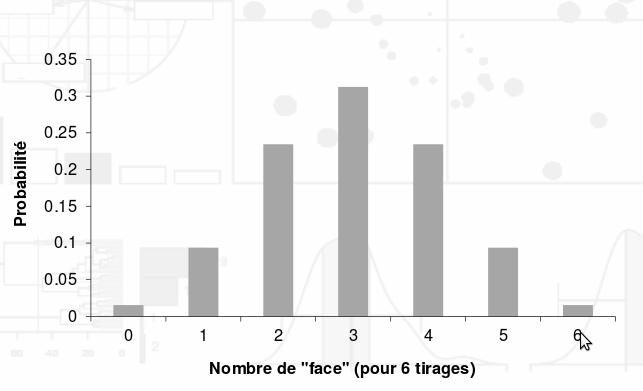
\includegraphics[scale=0.5]{ilu/g1.png}\caption{Probabilité d'obtention de face entre 0 et 6}\end{center}\end{figure}

Nous pouvons voir sur la figure ci dessus, la représentation de la distribution des probabilités calculées exactement pour chacune des possibilités.\newline
il y a plus de probabilités d'obtenir 3, exceptionnellement 1 ou 5 et très rarement 0 ou 6.\newline
On peut réitérer l'expérience sur 20 lancés.
\begin{figure}[H]\begin{center}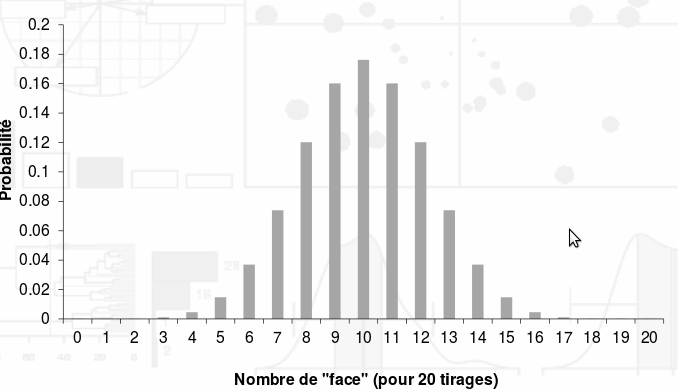
\includegraphics[scale=0.5]{ilu/g2.png}\caption{Probabilité d'obtention de face entre 0 et 20}\end{center}\end{figure}
il y a plus de probabilités d'obtenir 10, exceptionnellement 4 ou 14 et très rarement 2 17.\newline
\\
La distribution de cette Variable aléatoire prend une distribution très régulière et harmonieuse.\newline
Ainsi, quand le nombre de tirage ne tend plus vers 20 mais vers $+\infty$, la loi tend à se rapprocher d'une courbe continue que l'on appelle \textbf{Coubre de Gauss} ou \textbf{Courbe Normale}.

\begin{figure}[H]\begin{center}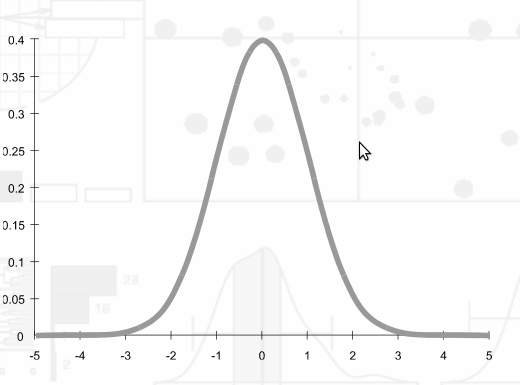
\includegraphics[scale=0.5]{ilu/g3.png}\caption{Représentation de la distribution de la loi Normale}\end{center}\end{figure}
La loi normale a une grande importance en statistique. En effet, quand une variable est la résultante d'un grand nombre de variable aléatoires indépendante, alors cette variable suit une \textbf{Loi Normale}; Par exemple, la taille d'un individu; elle est la résultante de plusieurs facteurs génétiques, environnementaux, sociaux et culturels, \dots L'ensemble de ces facteurs étant plus ou moins indépendants, on peut en conclure que la taille d'un individu suit une loi normale.\newline
\\
Partant de cette constatation, les statisticiens ont développé des tests optimaux, les plus performants possibles, pour analyser des variables aléatoires suivant des lois Normales.
\newpage
\section{Représentations graphiques}
Nous verrons successivement dans ce cours comment représenter les distributions de : 
\begin{itemize}
\item Variables qualitatives
\item Variables quantitatives
\item Diagrammes en bâtons, camemberts, histogrammes, boîtes à moustaches, diagrammes cartésiens, diagrammes en fagot.
\end{itemize}
Pendant ce cours, nous allons étudier le fichier \textit{smp1.csv}. Ce fichier est relatif à une étude sur la santé mentale en prison réalisée en 2004 et financée par les ministères de la justice et de la santé.\newline
Cette étude a portée sur 799 détenus masculins, tirés au sort dans les prisons de France métropolitaine.\newline
Dans ce fichier, nous avons un extrait de neuf variables : 
\begin{itemize}	
\item L'Age
\item La Profession du détenu 
\item L'existence d'un diagnostic de depression ou schizophrénie issu du consensus de deux clininciens 
\item Le Niveau de gravité éventuelle de la pathologie du détenu
\item Le nombre d'enfants du détenu 
\end{itemize} 
\textcolor{white}{.}\newline
Ainsi que trois variables relatives à la personnalité du détenu : 
\begin{itemize}
\item Le niveau de recherche de sensation (curiosité, attrait pour le risque et la nouveauté) noté \underline{rs}.
\item Le niveau d'évitement du danger (timidité, précautionneux) noté \underline{ed}
\item Le niveau de dépendance à la récompense (sensibilité aux relations sociales, influençable) noté \underline{dr}.
\end{itemize}
\subsection{Importation des données csv}
Nous allons importer le fichier csv : 
\begin{itemize}
\item \textit{read.csv2("/comptes/E131729J/XX\_Université\_fun/univfunR/TP/smp1.csv")} - Fonction d'import
\item \textit{str(smp.c)} - fonction de visulation des données
\end{itemize}

\begin{lstlisting}[language=html]
> smp.c <- read.csv2("/comptes/E131729J/XX_Université_fun/univfunR/TP/smp1.csv")
> ### A modifier sous MAC
> str(smp.c)
'data.frame':	799 obs. of  9 variables:
 $ age      : int  31 49 50 47 23 34 24 52 42 45 ...
 $ prof     : Factor w/ 8 levels "agriculteur",..: 3 NA 7 6 8 6 3 2 6 6 ...
 $ dep.cons : int  0 0 0 0 1 0 1 0 1 0 ...
 $ scz.cons : int  0 0 0 0 0 0 0 0 0 0 ...
 $ grav.cons: int  1 2 2 1 2 1 5 1 5 5 ...
 $ n.enfant : int  2 7 2 0 1 3 5 2 1 2 ...
 $ rs       : int  2 2 2 2 2 1 3 2 3 2 ...
 $ ed       : int  1 2 3 2 2 2 3 2 3 2 ...
 $ dr       : int  1 1 2 2 2 1 2 2 1 2 ...
\end{lstlisting}
\subsection{Variables qualitatives}
\subsubsection{Histogramme}
Un façon classique de représenter la distribution d'une variable aléatoire qualitative est d'utiliser un diagramme en bâtons. Avec \textbf{R}, il faut utiliser les fonctions : 
\begin{itemize}
\item \textit{table} - cette fonction va calculer le nombre de détenus ayant chacun des métier (en ayant précisé : smp.c\$prof) 
\item \textit{barplot} - cette fonction va représenter des bâtons avec pour hauteur, le nombre des détenus.
\end{itemize}
\begin{lstlisting}[language=html]
> table(smp.c$prof)
       agriculteur            artisan              autre              cadre 
                 6                 90                 31                 24 
           employe            ouvrier prof.intermediaire        sans emploi 
               135                227                 58                222 
> barplot(table(smp.c$prof))

\end{lstlisting}
\begin{figure}[H]\begin{center}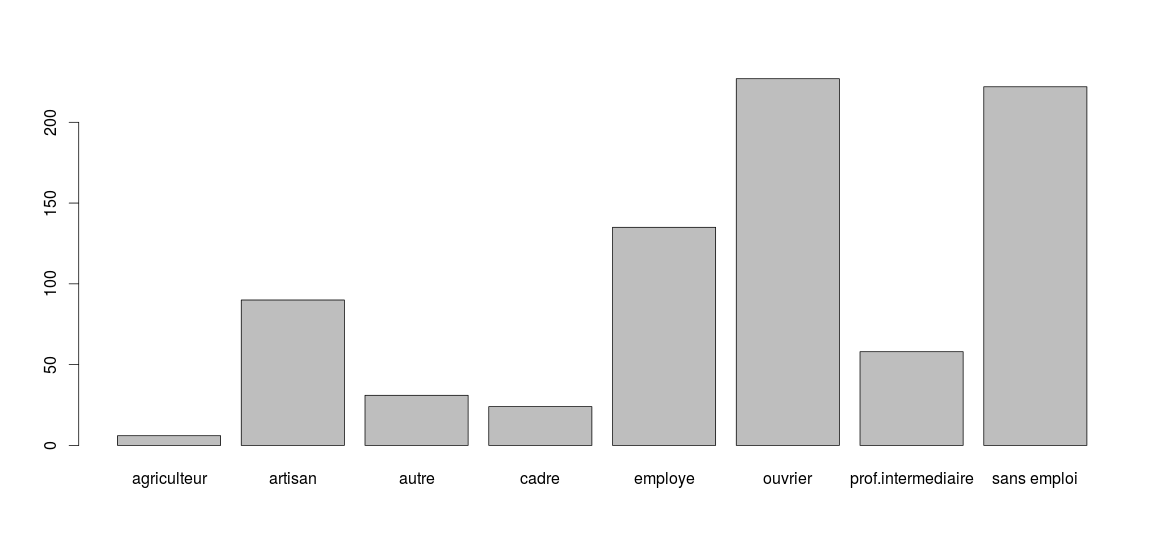
\includegraphics[scale=0.3]{ilu/tp1.png}\caption{Représentation sous forme d'un histogramme}\end{center}\end{figure}
\subsubsection{Pie chart}
Un autre grand classique pour représenter graphiquement la distribution d'une variable aléatoire catégorielle, c'est d'utiliser un camembert (Diagramme circulaire). Avec \textbf{R}, il faut utiliser les fonctions : 
\begin{itemize}
\item \textit{table} - cette fonction va calculer le nombre de détenus ayant chacun des métier (en ayant précisé : smp.c\$prof) 
\item \textit{pie} - cette fonction va représenter des diagrammes circulaires.
\end{itemize}
\textcolor{white}{.}\newline
\textbf{Note : }Certains statisticiens sont réticents à l'usage de tel diagrammes. En effet, Il semblerait que l'oeil humain ait des difficultés à percevoir intuitivement des rapports de surface entre des secteurs de cercle. Alors qu'au contraire, l'oeil humain sertait capable de percevoir intuitivement des hauteurs de bâtons dans un diagramme en bâtons. \newline
\\
En pratique, les représentation en camembert ont une certaine utilité quand on est intéressé par la part que représente une profession données par rapport à l'ensemble des détenu (schéma à transposer en cas étudié).  En effet, chaque secteur peut être comparé à la superficie totale du disque. \newline
Au contraire, avec un diagramme en bâtons, il faudrait ajouter un bâton qui représente (par somme), l'ensemble de l'effectif étudié, ce qui est très peu commode.
\begin{lstlisting}[language=html]
> table(smp.c$prof)

       agriculteur            artisan              autre              cadre 
                 6                 90                 31                 24 
           employe            ouvrier prof.intermediaire        sans emploi 
               135                227                 58                222 

> pie(table(smp.c$prof))
\end{lstlisting}
\textcolor{white}{.}\newline
\begin{figure}[H]\begin{center}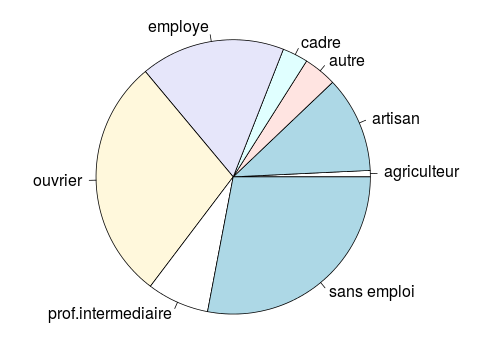
\includegraphics[scale=0.5]{ilu/tp2.png}\caption{Représentation sous forme d'un diagramme circulaire (camembert)}\end{center}\end{figure}
\subsection{Variables quantitatives}
\subsubsection{Histogramme}
Le grand classique pour représenter la distribution d'une variable aléatoire quantitative continue est \textbf{l'histogramme}.  \newline
\\
\textbf{Note :} Pour une variable aléatoire continue discrète, il vaut mieux utiliser un diagramme en bâtons.\newline
La différence entre les deux, c'est qu'avec l'histogramme, les bâtons sont contigus pour bien montrer qu'il y a une continuité dans les valeurs de la variable. \newline
Le seul point théorique un peu délicat avec un histogramme est de savoir comment il faut déterminer le nombre de bâtons. En pratique, avec \textbf{R}, c'est automatique et cela fonctione très bien 99 fois sur 100.\newline
l'instruction que nous allons utiliser est : 
\textcolor{white}{.}\newline
\begin{itemize}
\item \textit{hist(x)}, avec x, une variable que l'on souhaite représenter
\end{itemize}
\begin{lstlisting}[language=html]
> table(smp.c$age)

19 20 21 22 23 24 25 26 27 28 29 30 31 32 33 34 35 36 37 38 39 40 41 42 43 44 
45 46 47 48 49 50 51 15 15 18 13 23 30 22 30 25 21 20 25 18 22 26 20 16 18 25 
24 23 22 23 19 17 19 17 16 12 17 23 16 11 52 53 54 55 56 57 58 59 60 61 62 63 
64 65 66 67 68 69 70 71 72 73 74 77 79 81 83 10  8 11  6 14  9  7  6  7  5  7  
4  5  3  6  4  2  1  1  6  3  2  2  3  1  1  2 
> hist(smp.c$age)
\end{lstlisting}
\begin{figure}[H]\begin{center}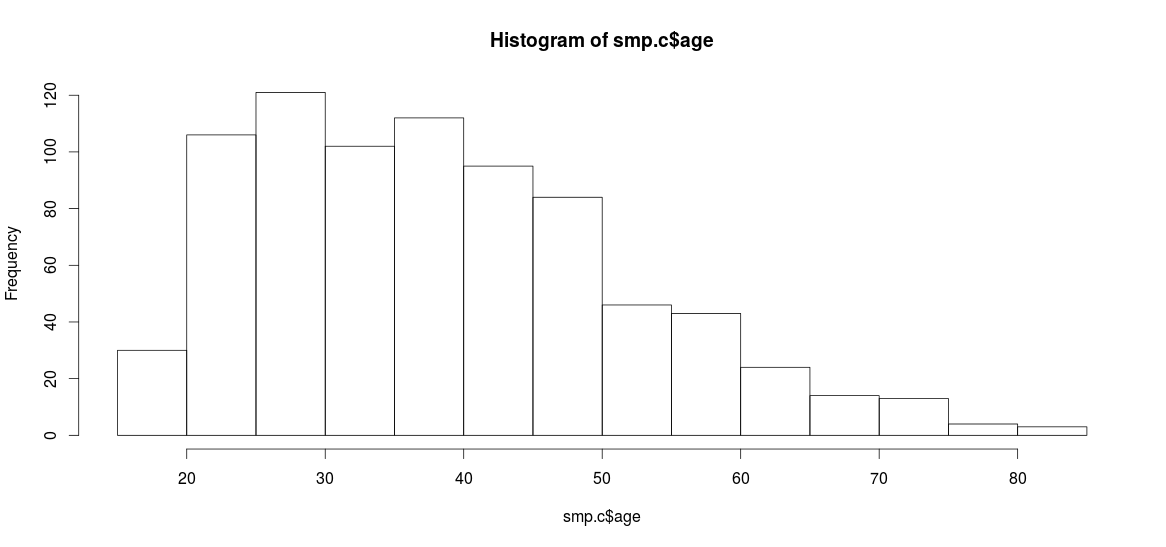
\includegraphics[scale=0.4]{ilu/tp3.png}\caption{Représentation sous forme d'un histogramme}\end{center}\end{figure}
\textbf{Attention : } Pour utiliser la fonction hist(), il faut que les valeurs à représenter soient de type numérique.\newline
\\
On peut être un peu dessus de l'aspect graphique et notamment, du fait que les bâtons ne soient pas grisés. Pour cela, il suffit d'ajouter des instruction à la fonction hist() comment par exemple : \textit{col="grey"}.
\begin{lstlisting}[language=html]
hist(smp.c$age,col="grey")
\end{lstlisting}
\begin{figure}[H]\begin{center}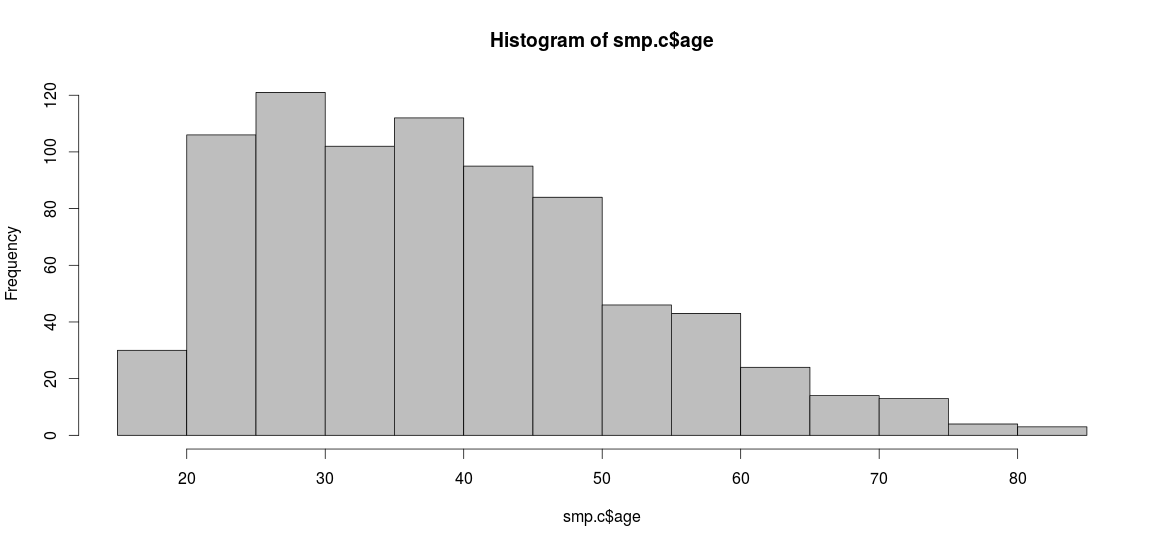
\includegraphics[scale=0.4]{ilu/tp3a.png}\caption{Représentation sous forme d'un histogramme}\end{center}\end{figure}
On peut également décider de changer le titre du graphique et de changer la légende de l'axe des x et des y. 
\begin{lstlisting}[language=html]
hist(smp.c$age,col="grey", main="Représentation des âges", xlab = "Age",, ylab="Fréquence")
\end{lstlisting}
\begin{figure}[H]\begin{center}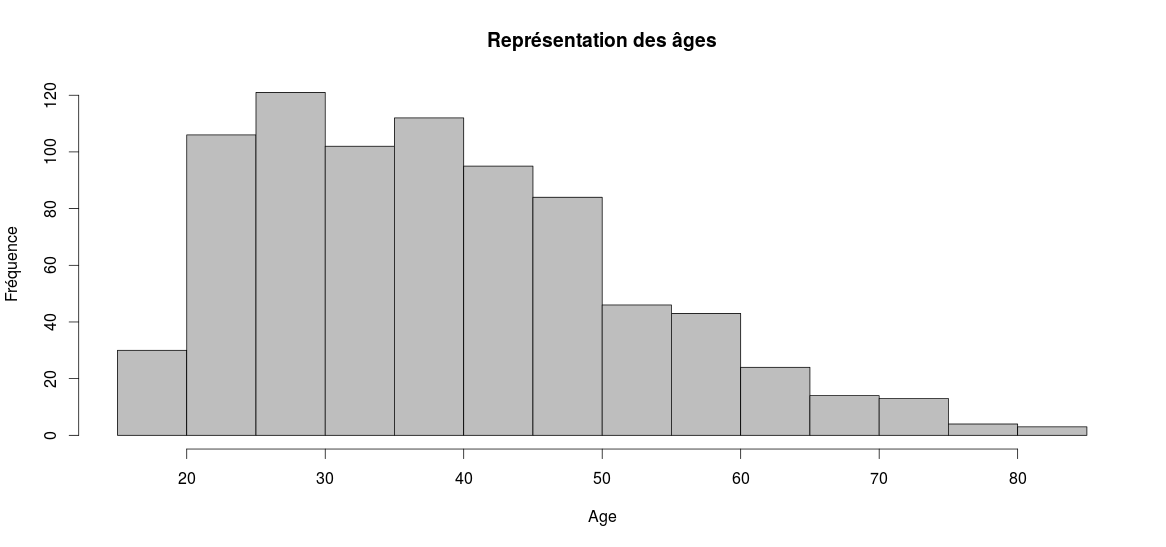
\includegraphics[scale=0.4]{ilu/tp3b.png}\caption{Représentation sous forme d'un histogramme}\end{center}\end{figure}
\textbf{Note : } Pour tout simplement supprimer le titre du graphique, il suffit d'ajouter la fonction \textit{main=""}
\begin{lstlisting}[language=html]
hist(smp.c$age,col="orange", main="", xlab = "Age",, ylab="Fréquence")
\end{lstlisting}
\textcolor{white}{.}\newline
\subsubsection{Boîte à moustaches - Box plot}
Une solution plus synthétique est de représenter graphiquement la répartition d'une variable aléatoire quantitative est d'utiliser une \textbf{boite à moustaches} (boîte de Tukey ou box plot).\newline
L'instruction dans \textbf{R} est : 
\begin{itemize}
\item \textit{boxplot(x)} avec x, une variable que l'on souhaite représenter.
\end{itemize}
\textcolor{white}{.}\newline
\textbf{Attention : } Une box plot ne peut représenter la distribution que de variables numériques.

\begin{lstlisting}[language=html]
boxplot(smp.c$age,col="pink", main="", xlab = "Age", ylab="")
\end{lstlisting}
\begin{figure}[H]\begin{center}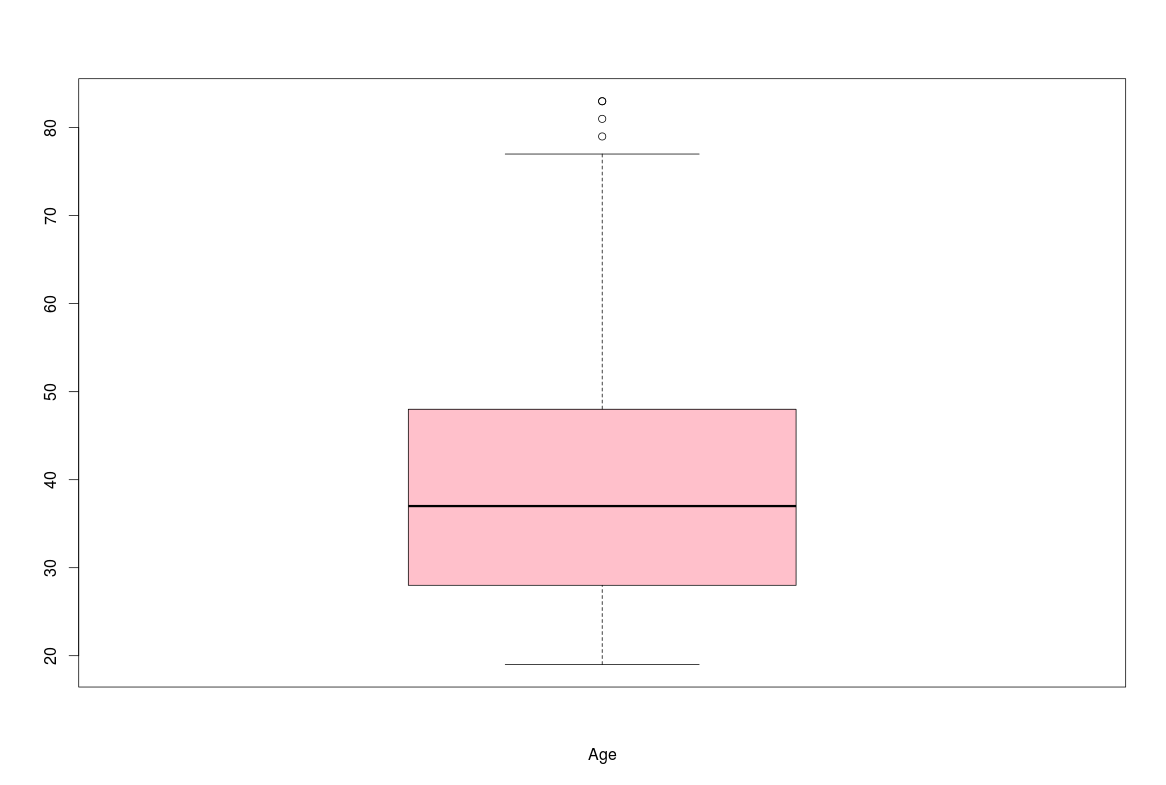
\includegraphics[scale=0.3]{ilu/tp4.png}\caption{Représentation sous forme d'une boite à moustaches}\end{center}\end{figure}
Une boîte à moustache s'interprète de la manière suivante : 
\begin{itemize}
\item \textit{A l'intértieur de la boite,} vous avez $\sim$ 50\% des données.
\item \textit{Entre le bord supérieur de la boite et la moustache supérieure,} vous avez $\sim$ 25\% des données.
\item \textit{Entre le bord inférieur de la boite et la moustache inférieure,} vous avez $\sim$ 25\% des données.
\item les données au dessus et en dessous des moustaches sont appelées \textit{outlayers} qui sont de données considérées comme aberrantes.
\end{itemize}
La présence des ces outlayers est expliqué par une imprécision dans la définition des ensembles donnés ci deçu. \newline
En effet, la moustache supérieure correspond :
$$\min(\max, q_{3} + 1.5 (q_{3}-q_{1}))$$
et, la moustache inférieure correspond :
$$\max(\min, q_{1} - 1.5 (q_{3}-q_{1}))$$
Les boîtes à moustaches sont réellement utiles pour représenter graphiquement la distribution d'une variable quantitative en fonction de sous groupes. Par exemple, on pourrait se demander : \textit{Est ce que la distribution de l'âge est la même selon que l'on ait un niveau de sensation faible, moyen ou élevé ?}\newline
La réponse avec \textbf{R} : 
\begin{lstlisting}[language=html]
> table(smp.c$age)
19 20 21 22 23 24 25 26 27 28 29 30 31 32 33 34 35 36 37 38 39 40 41 42 43 44 
45 46 47 48 15 15 18 13 23 30 22 30 25 21 20 25 18 22 26 20 16 18 25 24 23 22 
23 19 17 19 17 16 12 17 49 50 51 52 53 54 55 56 57 58 59 60 61 62 63 64 65 66 
67 68 69 70 71 72 73 74 77 79 81 83 23 16 11 10  8 11  6 14  9  7  6  7  5  7  
4  5  3  6  4  2  1  1  6  3  2  2  3  1  1  2 

> table(smp.c$rs)
  1   2   3 
249 158 289 
> boxplot(smp.c$age~smp.c$rs,col="pink", main="Corrélation entre l'âge et la recherche de sensation ?", xlab = "Recherche de sensation", ylab="Age")
\end{lstlisting}
\begin{figure}[H]\begin{center}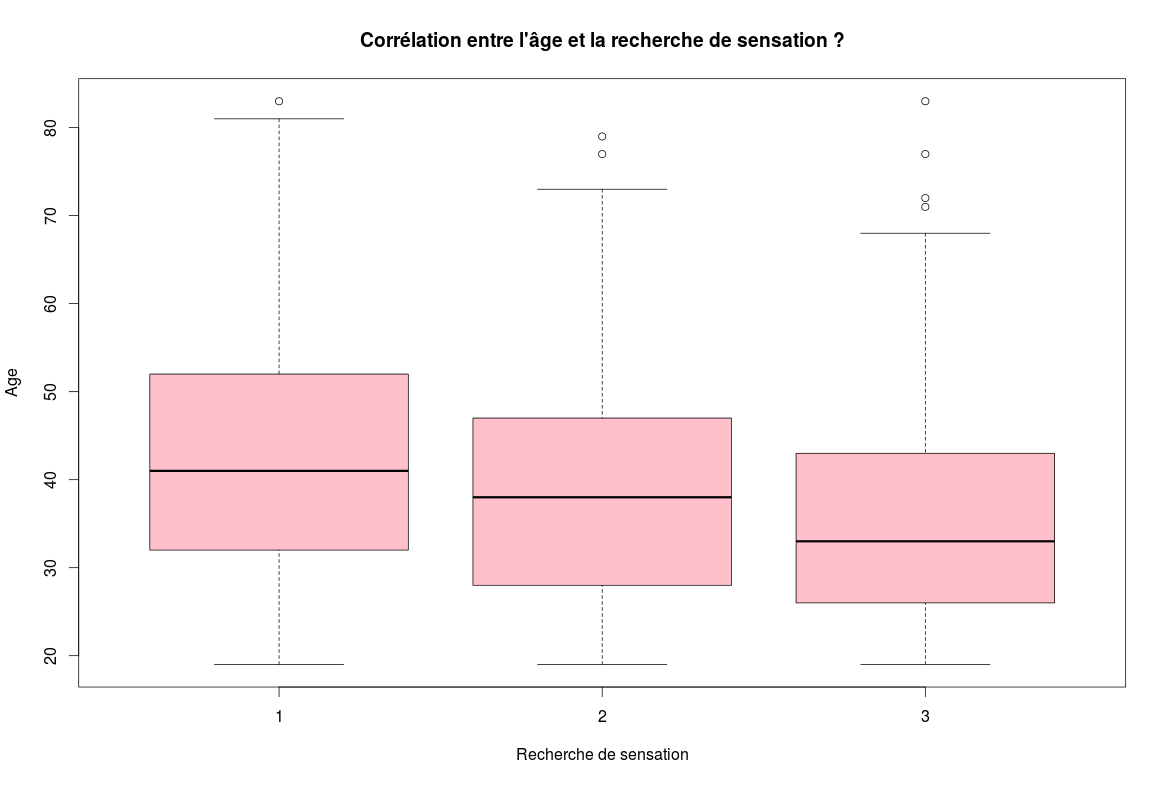
\includegraphics[scale=0.35]{ilu/tp5.png}\caption{Recherche d'influence de l'âge sur la recherche de sensation}\end{center}\end{figure}
\textit{Analyse :} On observe ici que glolement, la distribution de l'âge est légèrement supérieure quand on a un faible niveau de sensation plutot que lorsque l'on a un niveau de sensation élevé. \newline
\\
Pour représenter graphiquement la \underline{distribution conjointe} de deux variables aléatoires quantitatives à l'aide d'un graphique cartésien, il faut utiliser la fonction : 
\begin{itemize}
\item \textit{plot(x,y)} - avec x et y, respectivement, les varables aléatoires que l'on souhaite représenter sur l'axe de x et celui des y.
\end{itemize}
\textcolor{white}{.}\newline
Dans le cas suivant, nous allons représenter la distribution de l'âge et du nombre d'enfants et for logiquement, plus un detenu est âgé, plus il a en moyenne, un nombre d'enfant élevé :  

\begin{lstlisting}[language=html]
> table(smp.c$age)
19 20 21 22 23 24 25 26 27 28 29 30 31 32 33 34 35 36 37 38 39 40 41 42 43 44 
45 46 47 48 49 50 51 15 15 18 13 23 30 22 30 25 21 20 25 18 22 26 20 16 18 25 
24 23 22 23 19 17 19 17 16 12 17 23 16 11 52 53 54 55 56 57 58 59 60 61 62 63 
64 65 66 67 68 69 70 71 72 73 74 77 79 81 83 10  8 11  6 14  9  7  6  7  5  7  
4  5  3  6  4  2  1  1  6  3  2  2  3  1  1  2 

> table(smp.c$n.enfant)
  0   1   2   3   4   5   6   7   8   9  10  11  13 
214 220 125 101  55  31   7   7   7   2   2   1   1 
> plot(smp.c$age, smp.c$n.enfant,col="blue", main="", xlab = "Age", ylab="Nombre d'enfants")
\end{lstlisting}
\begin{figure}[H]\begin{center}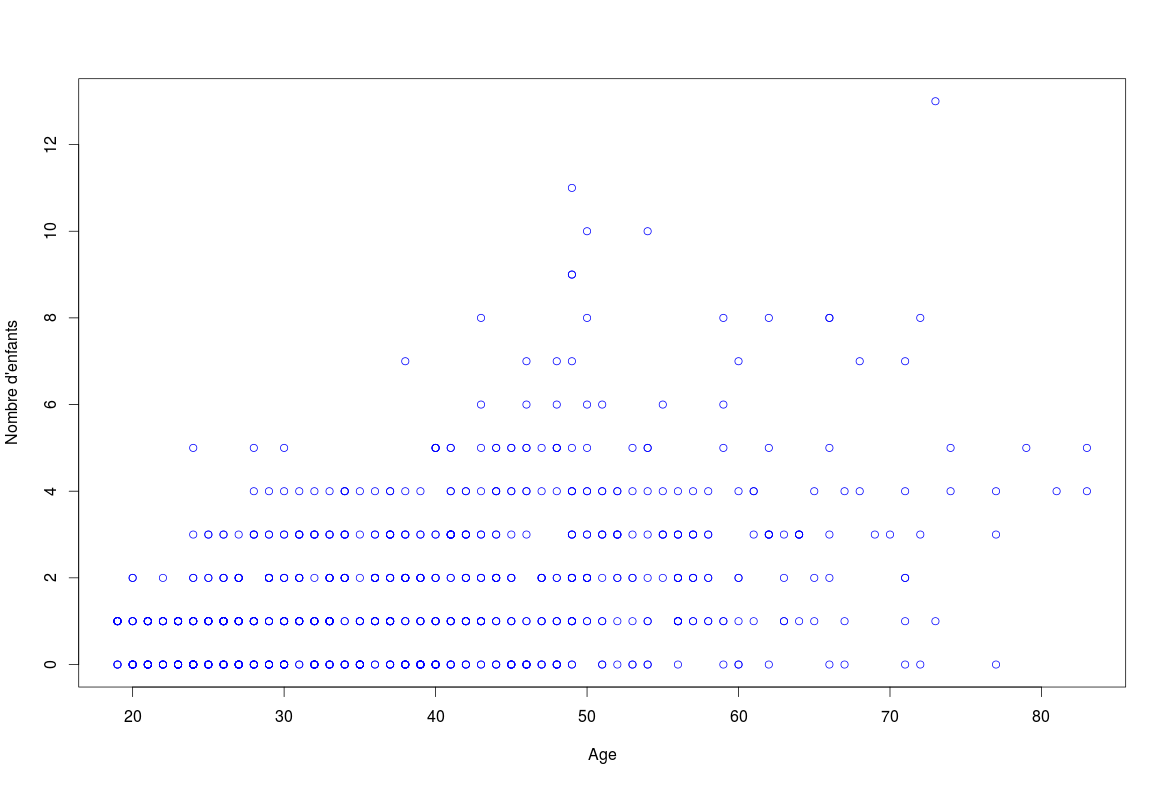
\includegraphics[scale=0.3]{ilu/tp6.png}\caption{Représentation d'une corrélation entre deux variables aléatoire à l'aide de la fonction plot(x,y)}\end{center}\end{figure}
On peut être étonné par le fait qu'un semble ne pas y avoir 800 points correspondants au 799 détenus et cela s'explique naturellement par le fait que deux détenus ayant chacun  50 ans et 2 enfants auront un point situé exactement au même endroit. Ca n'est pas gênant en soi mais cela peut induire en erreur (on peut avoir l'impression qu'il y a moins de sujets qu'il y en a réellement).\newline
Une façon de se tirer de ce faux pas est de bouger légèrement et de manière totalement aléatoire chaque point afin qu'ils se décollent les uns des autres.\newline
L'instruction correspondante est la fonction \textit{jitter()}.
\begin{lstlisting}[language=html]
plot(jitter(smp.c$age), jitter(smp.c$n.enfant),col="blue", main="", xlab = "Age", ylab="Nombre d'enfants")
\end{lstlisting}
\begin{figure}[H]\begin{center}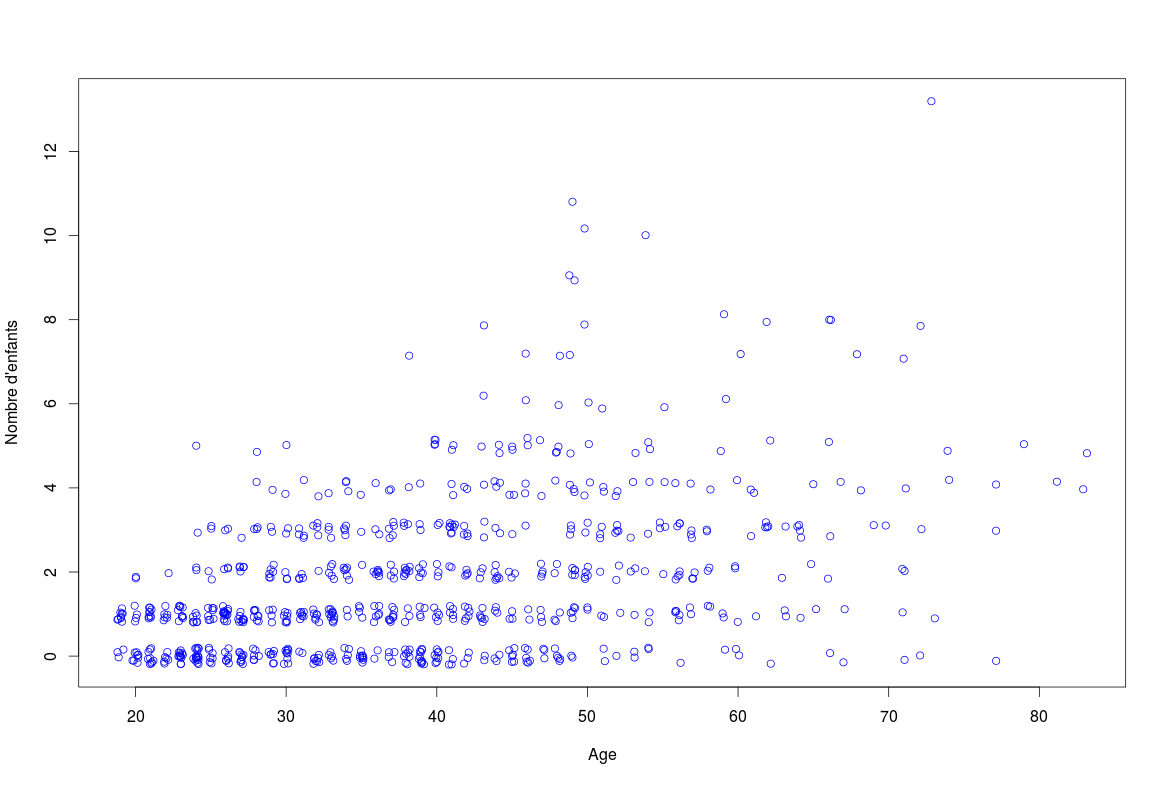
\includegraphics[scale=0.3]{ilu/tp7.png}\caption{Représentation d'une corrélation entre deux variables aléatoire à l'aide de la fonction plot(x,y) et l'instruction jitter()}\end{center}\end{figure}
Dès lors, nous avons un graphique plus agréable à regarder où cette fois, il y a bien 799 points.\newline
\\
Parfois, c'est l'évolution temporelle de la distribution d'une variable aléatoire quantitative que l'on veut représenter. Le diagramme correspondant s'appelle un \textbf{diagramme temporel} voire parfois diagramme de température. Le fichier que nous utilisons concernant la santé mentale en prison ne nous permet pas de réaliser des analyses temporelle; En effet, c'est une étude transversalle ayant été menée en un temps donnée. Il nous est donc impossible de représenter graphiquement l'évolution au cours du temps. \newline
Pour cela, nous allons étudier un nouveau fichier de données. Cette fois ci, nous allons étudier des patients déprimés, hospitalisés pour dépression et qui sont suivis pendant quelques semaines (hdrs.csv).\newline
\\
\begin{lstlisting}[language=html]
> smp.c <- read.csv2("/Users/mehdilatif/Desktop/DIVERS + TEMPLATES/R/TP/outils_hdrs.csv")
> str(smp.c)
'data.frame': 1053 obs. of  3 variables:
 $ NUMERO: int  96 96 96 96 96 96 96 96 157 157 ...
 $ VISIT : int  0 4 7 14 21 28 42 56 0 4 ...
 $ HDRS  : int  34 26 12 7 5 1 1 1 27 19 ...
> summary(smp.c)
     NUMERO           VISIT           HDRS      
 Min.   :  0.00   Min.   : 0.0   Min.   : 0.00  
 1st Qu.: 42.00   1st Qu.: 4.0   1st Qu.: 9.00  
 Median : 94.00   Median :14.0   Median :17.00  
 Mean   : 91.29   Mean   :20.4   Mean   :17.09  
 3rd Qu.:135.00   3rd Qu.:28.0   3rd Qu.:25.00  
 Max.   :191.00   Max.   :56.0   Max.   :44.00  
\end{lstlisting}
\textcolor{white}{.}\newline
L'instruction qui permet de représenter graphiquement  l'évolution du score de depression, ici c'est le \textit{hdrs} (Hamilton Depressive Rating Scale) est la fonction \textit{plotmeans()}.\newline
La fonction \textit{plotmeans()} ne fait pas partie du bagage standard \textbf{R} mais de la librairie \textit{gplots}. Pour pouvoir l'utiliser,, il faut d'abord installer le package \textit{gplots}. Il faut donc l'installer comme le présente l'image ci dessous : 
\begin{figure}[H]\begin{center}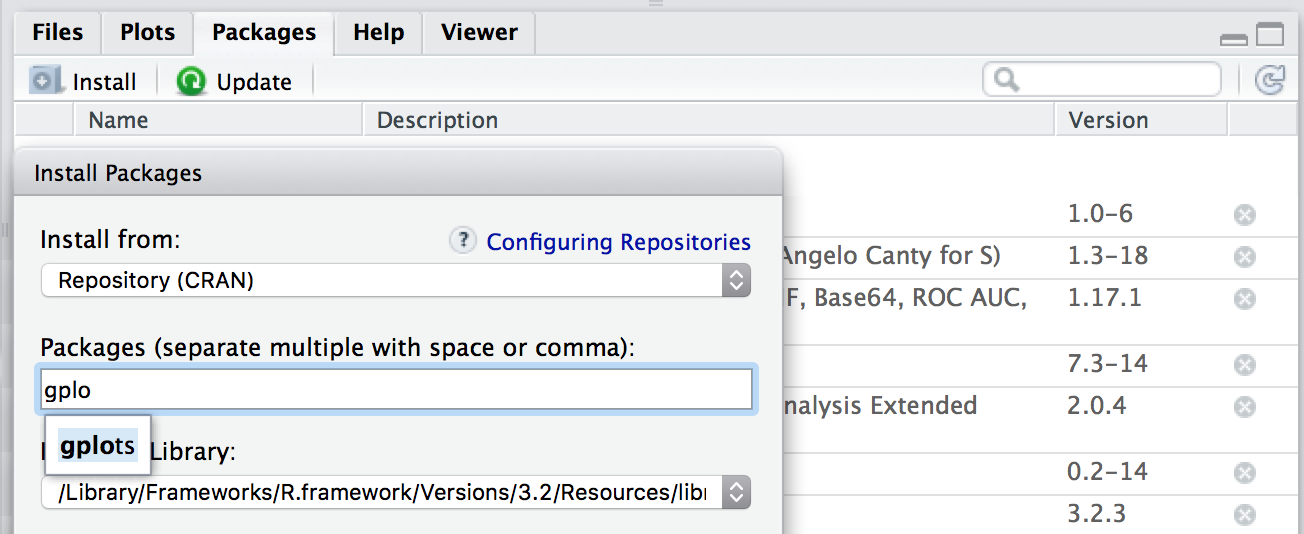
\includegraphics[scale=0.5]{ilu/tp8.png}\caption{Installation du package gplots}\end{center}\end{figure}
L'installation d'un package n'est à reéaliser qu'une seule fois.\newline
\\
Une fois l'installation du package réalisée, nous devons faire appel à la librairie de fonction gplots pour pouvoir utiliser la fonction \textit{plotmeans()}. Nous n'avons plus qu'à représenter la variable qui nous intéresse (HDRS) en fonction de la variable qui représente le temps (VISIT), les deux séparées d'un $\sim$. Les instructions \textit{gap} et \textit{barcol} ne sont là que pour rendre la représentation graphique plus agréable à regarder. 
\begin{lstlisting}[language=html]
> library(gplots)
> plotmeans (smp.c$HDRS~smp.c$VISIT,barcol="black",xlab = "Visites", ylab = "Hamilton Rating Depressive Scale")
\end{lstlisting}
\begin{figure}[H]\begin{center}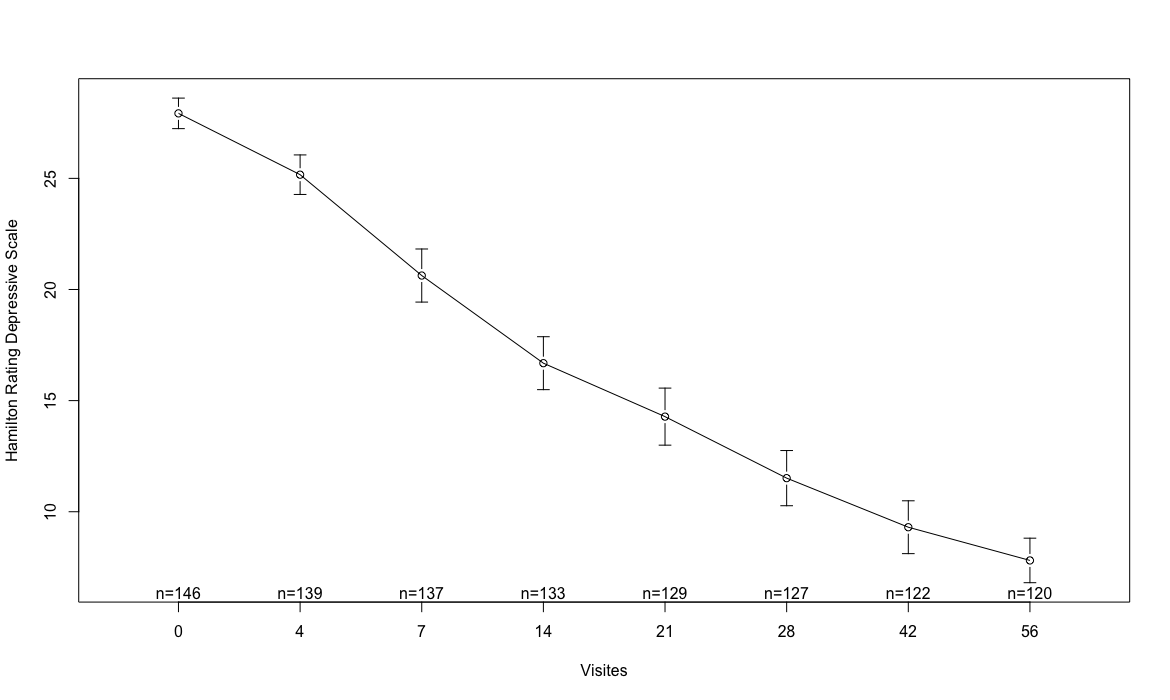
\includegraphics[scale=0.4]{ilu/tp9.png}\caption{Représentation du score HDRS moyen des patients en fonction des visites}\end{center}\end{figure}
Nous pouvons visualiser le fait que l'état symptomatique des patients s'améliore progressivement.\newline
\\
Plutôt que de représenter l'évolution moyenne des sujets au cours du temps, il peut être intéressant de représenter l'évolution de chaque sujet. Bien sûr, avec plusieurs centaines d'individus dans un jeu de données, l'ensemble peut être assez indigeste. Néanmoins, cela donne une impression intéressante de la variabilité de l'évolution d'un sujet à l'autre.\newline
La fonction correspondante est la fonction \textit{interaction.plot()}; Sa syntaxe est très simple, il faut : 
\begin{enumerate}
\item Définir la variable temporelle - dans notre exemple : VISIT
\item Définir la variable qui représente les sujets - dans notre exemple : NUMERO
\item Définit la variable qui représente l'information que l'on souhaite représenter : dans notre exemple : HDRS
\end{enumerate}
L'instruction \textit{lty=1} correspond au faut que nous voulons des lignes droites continues et \textit{legend} indique la légende.
\begin{lstlisting}[language=html]
> interaction.plot(smp.c$VISIT,smp.c$NUMERO,smp.c$HDRS, lty = 1, legend = FALSE)
\end{lstlisting}
\begin{figure}[H]\begin{center}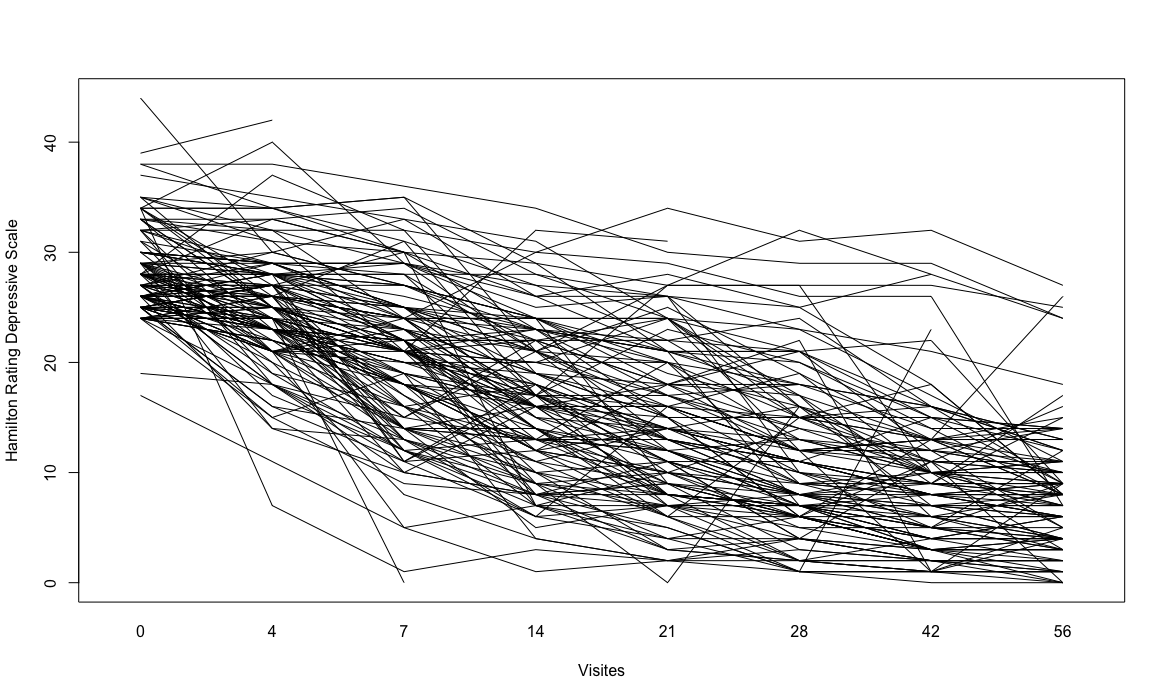
\includegraphics[scale=0.4]{ilu/tp10.png}\caption{Représentation du score HDRS de chaque patient patients en fonction des visites}\end{center}\end{figure}
\newpage
\section{Mesures de position et de dispersion, la théorie}
Au chapitre précédent sur les représentations graphiques, nous avons vu qu'un dessin pouvait représenter la distribution d'une variable aléatoire, quelle soit qualitative ou quantitative.\newline
Le problème, c'est que de nos jours, il n'est pas rare qu'un fichier de données contienne plusieurs centaines voire plusieurs millier de variables aléatoires. Il nous est donc impossible de faire 100 ou 1000 dessins; personne ne les lira, même pas l'investigateur.\newline
Nous avons donc besoin de mesures agrégées qui synthétisent l'information et qui la résume. De là, la notion de \textbf{mesures de dispersion et de mesures de position} parmis lesquelles, les très connus \textit{moyennes et écart types}.\newline
\\
Imaginez que vous ayez à travailler sur une étude visant à évaluer la consommation de Cannabis en France, selon que la population se situe autour d'un age de 15 ans ou 60 ans, la problématique de santé publique sous jacente, les déterminants de consommation vont être complètement différents. Il est donc indispensable de disposer d'un paramètre simple qui permet de dire immédiatement autoir de quel âge se situe la population. On appelle ça une mesure de position.\newline
En complément de cette mesure de position, on a besoin de connaitre la dispersion; Si vous prenez des adolescents et que vous les interrogez en classe de troisième, ils auront tous autour de 15 ans. Cependant, si vous interrogez en mélangeant collège et lycée, vous aurez des jeunes dont l'âge varie entre 11 et 18 ans, la problématique sera complètement différente.\newline
\\
Nous allons donc voir dans ce chapitre, des mesures de positions et de dispersions. Pour le cas de variables catégorielles, les mesures de positions sont assez simples à mettre en place, il suffit de lister les pourcentage de toute les modalités de catégories de la variable qualitative ou catégorielle évaluée.\newline
Pour une variable quantitative, c'est un petit peu plus compliqué et vous savez qu'il existe deux paramètres, la moyenne et la médiane.\newline
En ce qui concerne les mesures de dispersion, on utilise les notion de quartiles et d'ecart- type (Ce dernier, très connu mais pas forcément facile à utiliser car son interprétation est délicate). 
\subsection{Mesures de position}
\subsubsection{Moyenne et médiane}

\begin{figure}[H]\begin{center}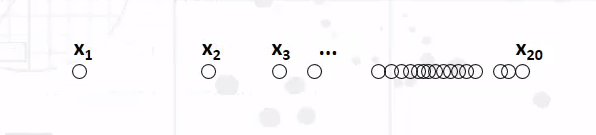
\includegraphics[scale=0.5]{ilu/g4.png}\end{center}\end{figure}
Considérons donc une variable avec une vingtaine d'observations. L'objectif est de trouver une valeur autour de laquel se situe globalement l'ensemble des observations. \newline
\\ La première solution, la plus classique, serait de calculer la \textbf{moyenne}, c'est à dire faire : 
$$\frac{1}{\textrm{nombre d'Observation}}\sum_{i=1}^{i=20} x_{i}$$
On est conditionné depuis l'école primaire à avoir la moyenne de nos résultats qu'elle soit pondérée ou non.  Bref, dans la vie de tous les jours, on utilise des moyennes et on ne se rend même plus compte qu'en réalité, le \underline{sens à donner au moyenne n'est pas si évident que ça}.\newline 
\\
\textbf{Exemple :} Vous avez eu 15 notes et la moyenne de ces 15 notes et 12, Qu'est ce que cela signifie ?\newline
Il est impossible de savoir si il y a plus de notes supérieures à 12 que de notes inférieures à 12 ou le contraire.\newline
\\
Un façon de se représenter géométriquement la moyenne est de considérer qu'elle est le barycentre de l'ensemble des observations. La moyenne ainsi un sens physique. \newline
Elle n'est pas le seul paramètre que l'on peut utiliser.\newline
\\
Il existe aussi la \textbf{médiane}. La médiane a un sens beaucoup plus clair : \textit{50\% des observations lui sont plus petites et 50\% des observations lui sont plus grandes.}\newline
\begin{figure}[H]\begin{center}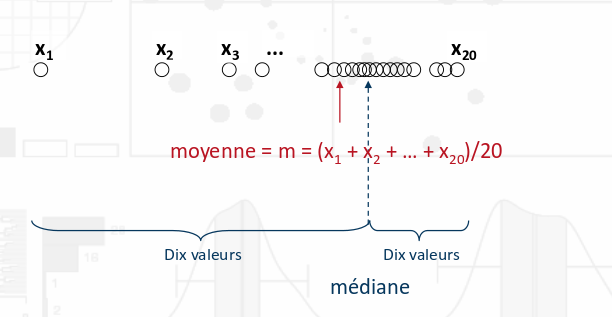
\includegraphics[scale=0.5]{ilu/g5.png}\end{center}\end{figure}
Si la \textbf{distribution est symétrique}, alors la médiane est égale à la moyenne. Sinon, et c'est la situation présente dans le graphique présenté ci dessus où l'onvoit que les observations sont beaucoup plus dispersées à gauche qu'à droite, alors il y a des différences non négligeables entre la moyenne et la médiane.\newline
\\
Mais en pratique, est il plus intéressant d'utiliser des médianes ou des moyennes ?\newline
\subsubsection{Avantages et inconvénients}

\paragraph{La médiane :} La médiane possède tout d'abord un côté \textbf{intuitif}; Au moins, nous savons ce que cela signifie (50 \% des valeurs plus grandes et 50\% des valeurs plus petites). \newline
On peut également parler de la \textbf{robustesse} de cette mesure. En effet, la médiane est très peu sensible au valeurs extrêmes. Sur un jeu de données contenant 50 sujets dont on analyse l'âge, si il y à une erreur de saisie (25 ans devient 2500 ans), alors la médiane ne va pas changer puisque cette dernière coupe juste l'échantillon en deux. Que les valeurs extrêmes soient hyper extrêmes ou peu extrêmes, cela ne changera rien à la médiane alors que ça impactera fortement la moyenne. \newline
La médiane est donc un paramètre robuste.
\paragraph{La moyenne : } Tout d'abord, ce paramètre est \textbf{simple a calculer} (somme des observations sur nombre d'observation) alors que la médiane n'est pas du tout aussi simple. En effet, avant de calculer une médiane, il faut au préalable, avoir classé l'ensemble des observations dans une ordre définit ou naturel.\newline
De plus, la moyenne possède une propriété géométrique et physique; c'est le \textbf{barycentre ou le centre de gravité} de la distribution.\newline
Autant la médiane n'est pas un "beau" paramètre en termes mathématiques, la moyenne a des propriétés mathématiques intéressantes.	\newline
Au delà des propriétés mathématiques, la moyenne à un \textbf{intérêt comptable} . On dit traditionnellement que pour représenter une variable qui a une distribution asymétrique ou assez fortement asymétrique, il faudrait utiliser une médiane et non une moyenne; et bien ce n'est pas toujours vrai. Prenons pour exemple la distribution de la durée de séjour de patients hospitalisés. On suppose que les patients vont être hospitalisés seulement quelques jours et puis, quelques-uns d'entre eux vont rester, à cause de complications, plusieurs semaines, voire plusieurs mois, mais ils sont très rares. Il serait logique donc, pour essayer d'avoir un paramètre de position de la durée de séjour d'avoir la médiane. Or les directeurs d?hôpitaux s'intéressent à la durée moyenne de séjour. En effet, si vous avez la durée moyenne de séjour et que vous connaissez le nombre de séjours hospitaliers annuels. quand vous multipliez l'un par l'autre, vous avez directement le nombre de jour de lits de lits d'hospitalisation occupés dans l'année et si l?hôpital est payé qu'au nombre de jours de lits d'hospitalisation occupés, alors le directeur d'hôpital sait exactement combien il va gagner sur son année.
\subsection{Mesures de dispersion}
Analysons maintenant les paramètres de dispersion. \newline
Nous considérons toujours les 20 observations de notre variable aléatoire
et dans un premier temps, nous nous intéresser à l'intervalle inter quartile.
\begin{figure}[H]\begin{center}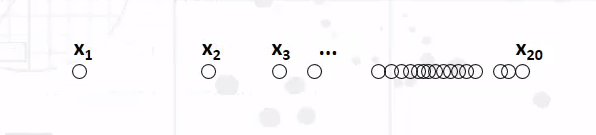
\includegraphics[scale=0.5]{ilu/g4.png}\end{center}\end{figure}
\subsubsection{Quartiles, écart-type}
La médiane découpait le jeu d'observartions en deux parts égales alors que les \textbf{Quartiles} découpent ce même jeu d'observations en quatres parts égales.
\begin{figure}[H]\begin{center}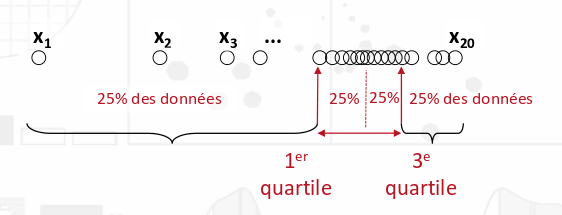
\includegraphics[scale=0.5]{ilu/g6.png}\end{center}\end{figure}
Il y a 25\% des sujets qui sont inférieurs au premier quartile ($q_{1}$),  25\% des sujets qui sont superieurs au troisième quartile ($q_{3}$) et donc entre $q_{1}$ et $q_{3}$, \textbf{l'espace interquartile}, nous avons 50\% des observations; ce sont les 50\% qui se regroupent autours de la médiane. \textbf{l'intervalle interquartile} a ainsi un sens clair et immédiat : \textbf{il regroupe la moitié de l'échantillon qui se situe autour de la médiane}. On se rappelle des boites à moustaches : 
\begin{figure}[H]\begin{center}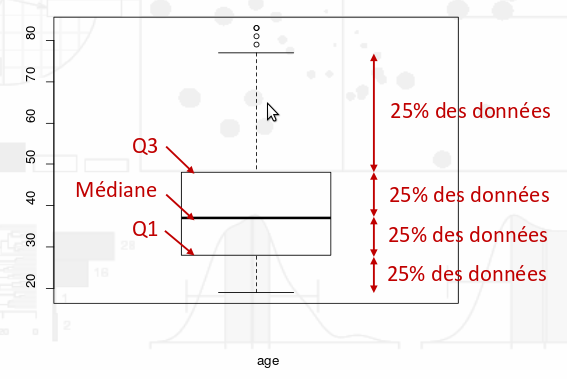
\includegraphics[scale=0.5]{ilu/g7.png}\end{center}\end{figure}
L'intervalle interquartile n'est pas le paramètre de dispersion le plus utilisé. On préfère en effet utiliser l'écart-type.\newline 
Par définition l'écart-type se calcule de la manière suivante :
$$\sigma^{2} = \textrm{Var} = \frac{1}{n} \sum_{x_{i} -\bar{x}}$$
$$\sigma = \sqrt{ \frac{1}{n} \sum_{x_{i} -\bar{x}}}$$
En pratique, cela ne veut rien dire \dots.
L'écart-type n'a aucun sens intuitif alors pourquoi utiliser un tel paramètre ? \newline
\\
Une première explication, c'est qu'à l'instar de la moyenne, l?écart-type à une certaine interprétation physique : il correspond à l?inertie. De la même façon l'écart-type a d'excellentes propriétés mathématiques (on le retrouve dans beaucoup de tests statistiques). Ce dernier étant également totalement différent de l'espace inter quartile qui, comme la médiane, n'a pas du tout de bonnes propriétés mathématiques.\newline
Enfin, l'écart-type possède une propriété qui le rend très utile et très simple à calculer : l'écart-type au carré, c'est à dire la variance, correspond à la moyenne des carrés moins la moyenne au carré :
$$\sigma^{2} = \frac{(x_{1}+ \dots +x_{20})^{2}}{20} - (\frac{x_{1}+ \dots +x_{20}}{20})^{2}$$
Nous allons voir qu'au début du $XX^{e}$ siècle, cette propriété fantastique.\newline 
\paragraph{Comment calculer la variance :}
Calcul de la variance \textbf{Old School}
\begin{center}

\begin{tabular}{lllllll}
\cline{1-4}
\multicolumn{1}{|l|}{$x_{i}$} & \multicolumn{1}{l|}{$\sum x_{i}$} & \multicolumn{1}{l|}{$x_{i}^{2}$} & \multicolumn{1}{l|}{$\sum x_{i}^{2}$} &  &  &  \\ \cline{1-4}
$x_{1}$                       & $s_{1}$                           & $x_{1}^{2}$                      & $q_{1}$                               &  &  &  \\
$x_{2}$                       & $s_{2}$                           & $x_{2}^{2}$                      & $q_{2}$                               &  &  &  \\
\dots                         & \dots                             & \dots                            & \dots                                 &  &  &  \\
$x_{1000}$                    & $s_{1000}$                        & $x_{1000}^{2}$                   & $q_{1000}$                            &  &  &  \\
                              &                                   &                                  &                                       &  &  & 
\end{tabular}
\end{center}
Avec $$s_{2} = \sum_{i=1}^{2} x_{i} = x_{1} + x_{2}= s_{1}+s_{2} $$
Et $$q_{2} = \sum_{i=1}^{2} x_{i}^{2} = x_{1}^{2} + x_{2}^{2} = q_{1}+q_{2}$$
\textit{Principe de la somme cumulative}\newline
\\
Le calcul de la variance s'effectue donc de la manière suivante : 
$$\textrm{Var} = \frac{q_{1000}}{1000} - (\frac{s_{1000}}{1000})^{2}$$
$$\sigma = \sqrt{\textrm{Var}} = \sqrt{\frac{q_{1000}}{1000} - (\frac{s_{1000}}{1000})^{2}}$$
Cette formule permet donc de simplifier le calcul de la variance mais également de l'écart-type puisque l'on a qu'une racine carré à calculer (à l'époque, ils n'avaient pas de calculatrice).\newline
\\ 
Imaginons qu'après le calcul terminé, on se rend compte qu'il manque une valeur, \textbf{NO PANIC} : 

\begin{center}
\begin{tabular}{lllllll}
\cline{1-4}
\multicolumn{1}{|l|}{$x_{i}$} & \multicolumn{1}{l|}{$\sum x_{i}$} & \multicolumn{1}{l|}{$x_{i}^{2}$} & \multicolumn{1}{l|}{$\sum x_{i}^{2}$} &  &  &  \\ \cline{1-4}
$x_{1}$                       & $s_{1}$                           & $x_{1}^{2}$                      & $q_{1}$                               &  &  &  \\
$x_{2}$                       & $s_{2}$                           & $x_{2}^{2}$                      & $q_{2}$                               &  &  &  \\
\dots                         & \dots                             & \dots                            & \dots                                 &  &  &  \\
$x_{1000}$                    & $s_{1000}$                        & $x_{1000}^{2}$                   & $q_{1000}$                            &  &  &  \\
\textcolor{red}{$x_{1001}$}                    & \textcolor{red}{$s_{1001}$ }                      & \textcolor{red}{$x_{1001}^{2}$}                  & \textcolor{red}{$q_{1001}$}                          &  &  &
\end{tabular}
\end{center}

$$\textrm(Var) = \frac{q_{1000}+x_{1001}^{2}}{1001} - (\frac{s_{1000}+x_{1001}}{1001})^{2}$$
$$\sigma = \sqrt{\textrm{Var}} = \sqrt{\frac{q_{1000}+x_{1001}^{2}}{1001} - (\frac{s_{1000}+x_{1001}}{1001})^{2}}$$
\subsubsection{Que penser d'un écart-type}
Au total, l'écart-type est principalement utilisé pour ses propriétés mathématiques et calculatoires mais pas dans le sens qu'on pourrait intuitivement lui donner.\newline
En effet, l'écart type est utilisé dans le calcul suivant :\newline
\\
\textit{Si la variable à une distribution normale, l'intervalle qui contient $[\bar{x}-\sigma, \bar{x}+\sigma]$ représente approximativement les $2/3$ des données (c'est à dire la majorité des données de la distribution)}.\newline
\newpage
\section{Mesures de position et de dispersion, la pratique}
Pour calculer tous ces paramètres dans \textbf{R}, il suffit d'utiliser la fonction \textit{summary}. Le logiciel va automatiquement retourner : 
\begin{itemize}
\item Pour les variables qualitatives
\begin{itemize}
\item le minimum,
\item le 1 er quartile,
\item la médiane,
\item la moyenne,
\item le 3 ème quartile,
\item le maximum
\item le nombre de données manquantes, il est très important de connaître le nombre de données manquantes pour chaque variable.
\end{itemize}
\item Pour les variables catégorielles

\begin{itemize}
\item le nombre de sujets pour chaque modalité
\item les données manquantes
\end{itemize}
\end{itemize}
\begin{lstlisting}[language=html]
> smp.c <- read.csv2("/Users/mehdilatif/Desktop/DIVERS + TEMPLATES/R/TP/outils_hdrs.csv")
> str(smp.c)
'data.frame':	799 obs. of  9 variables:
 $ age      : int  31 49 50 47 23 34 24 52 42 45 ...
 $ prof     : Factor w/ 8 levels "agriculteur",..: 3 NA 7 6 8 6 3 2 6 6 ...
 $ dep.cons : int  0 0 0 0 1 0 1 0 1 0 ...
 $ scz.cons : int  0 0 0 0 0 0 0 0 0 0 ...
 $ grav.cons: int  1 2 2 1 2 1 5 1 5 5 ...
 $ n.enfant : int  2 7 2 0 1 3 5 2 1 2 ...
 $ rs       : int  2 2 2 2 2 1 3 2 3 2 ...
 $ ed       : int  1 2 3 2 2 2 3 2 3 2 ...
 $ dr       : int  1 1 2 2 2 1 2 2 1 2 ...
> summary(smp.c)
      age                       prof        dep.cons         scz.cons        grav.cons    
 Min.   :19.0   ouvrier           :227   Min.   :0.0000   Min.   :0.0000   Min.   :1.000  
 1st Qu.:28.0   sans emploi       :222   1st Qu.:0.0000   1st Qu.:0.0000   1st Qu.:2.000  
 Median :37.0   employe           :135   Median :0.0000   Median :0.0000   Median :4.000  
 Mean   :38.9   artisan           : 90   Mean   :0.3967   Mean   :0.0826   Mean   :3.643  
 3rd Qu.:48.0   prof.intermediaire: 58   3rd Qu.:1.0000   3rd Qu.:0.0000   3rd Qu.:5.000  
 Max.   :83.0   (Other)           : 61   Max.   :1.0000   Max.   :1.0000   Max.   :7.000  
 NA's   :2      NA's              :  6                                     NA's   :4      
    n.enfant            rs              ed              dr       
 Min.   : 0.000   Min.   :1.000   Min.   :1.000   Min.   :1.000  
 1st Qu.: 0.000   1st Qu.:1.000   1st Qu.:1.000   1st Qu.:1.000  
 Median : 1.000   Median :2.000   Median :2.000   Median :2.000  
 Mean   : 1.755   Mean   :2.057   Mean   :1.866   Mean   :2.153  
 3rd Qu.: 3.000   3rd Qu.:3.000   3rd Qu.:3.000   3rd Qu.:3.000  
 Max.   :13.000   Max.   :3.000   Max.   :3.000   Max.   :3.000  
 NA's   :26       NA's   :103     NA's   :107     NA's   :111    
> 
\end{lstlisting}
Il existe également une autre fonction qui permet de résumer l'ensemble des informations concernant des variables aléatoires de manière plus claire: la fonction \textbf{describe()} qui se trouve dans le package \textit{prettyR}
\begin{lstlisting}[language=html]
> setwd("~/XX_Université_fun/univfunR/TP")
> outil <-read.csv2("/comptes/E131729J/XX_Université_fun/univfunR/TP/outils_hdrs.csv")
> str(outil)
'data.frame':	1053 obs. of  3 variables:
 $ NUMERO: int  96 96 96 96 96 96 96 96 157 157 ...
 $ VISIT : int  0 4 7 14 21 28 42 56 0 4 ...
 $ HDRS  : int  34 26 12 7 5 1 1 1 27 19 ...
> summary(outil)
     NUMERO           VISIT           HDRS      
 Min.   :  0.00   Min.   : 0.0   Min.   : 0.00  
 1st Qu.: 42.00   1st Qu.: 4.0   1st Qu.: 9.00  
 Median : 94.00   Median :14.0   Median :17.00  
 Mean   : 91.29   Mean   :20.4   Mean   :17.09  
 3rd Qu.:135.00   3rd Qu.:28.0   3rd Qu.:25.00  
 Max.   :191.00   Max.   :56.0   Max.   :44.00  
> library(prettyR)
> describe(outil)
Description of outil 

 Numeric 
        mean median     var    sd valid.n
NUMERO 91.29     94 2780.79 52.73    1053
VISIT  20.40     14  327.55 18.10    1053
HDRS   17.09     17   87.90  9.38    1053
\end{lstlisting}
La fonction \textbf{describe()} étant très intéressante, elle ne présente néanmoins ni les quartiles, ni les maximum et minimum; données absolument indispensables car lorsque vous présenterez un fichier, les valeurs minimales et maximales vous permettrons de détecter les données abérantes. Par exemple, si vous avez la variable \textit{smp\$age} et que vous détectez une erreur de mesure \textbf{e.g} max = 1596 ans.\newline
\textbf{Cependant,} on peut demander à la fonction \textbf{describe()} d'effectuer d'autres calculs que ceux proposés de base. Par exemple ,nous allons demander à la fonction de calculer les paramètres suivants : 
\begin{itemize}
\item moyenne
\item écart-type
\item variance
\item la médiane
\item le minimum
\item le maximum
\item le nombre de sujets dans l'échantillon
\end{itemize}
\begin{lstlisting}[language=html]
> library(prettyR) #Describe
> describe(outil, num.desc =c("mean","sd","var","median","min","max","valid.n"))
Description of outil 

 Numeric 
        mean    sd     var median min max valid.n
NUMERO 91.29 52.73 2780.79     94   0 191    1053
VISIT  20.40 18.10  327.55     14   0  56    1053
HDRS   17.09  9.38   87.90     17   0  44    1053
\end{lstlisting}
Il est possible de demander à la fonction de retourner les valeurs des quantiles pour n'importe quelle valeur de ce dernier.\newline
Comme nous l'avons vu en CM, il est possible également d'afficher le skewness représentant le coefficient de dissymétrie et le kurtosis représentant le coefficient d'aplatissement.
\begin{lstlisting}[language=html]
> library(prettyR) #Describe
> library(moments) #pour skewness et kurtosis
> describe(outil, num.desc =c("mean","sd","var","median","min","max","valid.n","skewness","kurtosis","q25","q75"))
Description of outil 

 Numeric 
        mean    sd     var median min max valid.n skewness kurtosis q25
NUMERO 91.29 52.73 2780.79     94   0 191    1053     0.07     1.81  42
VISIT  20.40 18.10  327.55     14   0  56    1053     0.72     2.30   4
HDRS   17.09  9.38   87.90     17   0  44    1053     0.06     1.98   9
       q75
NUMERO 135
VISIT   28
HDRS    25
\end{lstlisting}
Il est parfois très utile de calculer simplement les valeurs de la moyenne ou de l'écart type. Il existe des fonctions permettant de retourner ces valeurs : 
\textbf{mean()} pour la moyenne et \textbf{sd()} pour l'écart type. Il en est de même pour les fonctions de bases type min, max, cov, \dots Elle seront présentées plus en détail dans le TP de Probabilités discrètes.\newline
\\
Et pour une variable catégorielle, si vous voulez connaître les modalités, vous pouvez utiliser la fonction table(). La fonction table() est ici utilisée avec les options \textit{deparse.level=2}. Ça permet d'avoir le nom de la variable affiché et puis useNA qui est utilisé ici pour pouvoir savoir combien de sujets ont eu des données manquantes pour leurs professions
\begin{lstlisting}[language=html]
> smp <-read.csv2("/comptes/E131729J/XX_Université_fun/univfunR/TP/smp1.csv")
> mean(smp$age)
[1] NA
> mean(smp$age, na.rm = TRUE)
[1] 38.89962
> sd(smp$age)
[1] NA
> sd(smp$age, na.rm = TRUE)
[1] 13.28098
> table(smp$prof, deparse.level = 2, useNA = "always")
smp$prof
       agriculteur            artisan              autre 
                 6                 90                 31 
             cadre            employe            ouvrier 
                24                135                227 
prof.intermediaire        sans emploi               <NA> 
                58                222                  6 
\end{lstlisting}
\newpage
\section{Intervalles de confiance}
\subsection{Introduction}
Nous avons calculé les pourcentages, des moyennes, par exemple dans notre échantillon de détenus masculins pris en France métropolitaine; Nous avons environ 40\% de l'échantillon qui présentent une symptomatologie dépressive.En termes spécialisés, on dira que la prévalence de la symptomatologie dépressive est autour de 40\%.\newline
Nous avons également une moyenne d'âge d'environ 39 ans. Mais ces données, représentent la prévalence du symptôme dépressif et la moyenne d'âge pour nos 799 détenus. (\textit{et on doit bien avouer que l'on s'en fiche un peu}.)\newline
Ce qui nous intéresse, c'est d'étendre cette étude sur la population totale des détenus en France Métropolitaine.\newline
\\
Comment passer de résultats que l'on a estimé sur un échantillon donné à des résultats que l'on imagine exister dans la population totale des détenus.\newline
\\
C'est pour répondre à cette question que nous allons calculer des \textbf{Intervalles de confiance}.\newline
\begin{figure}[H]\begin{center}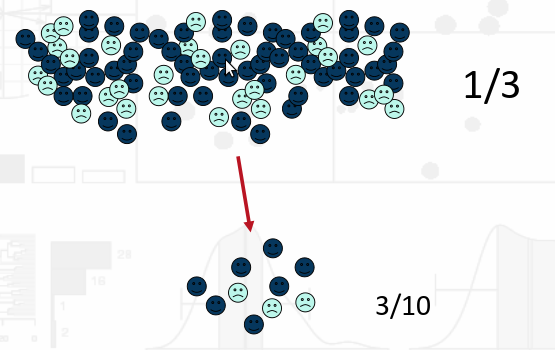
\includegraphics[scale=0.35]{ilu/bo.png}\end{center}\end{figure}
Imaginons que nous ayons une population de détenus. On sait que $\frac{1}{3}$ de ces derniers ont une symptomatologie dépressive.\newline
On en tire au sort $10$ et on constate, en les interrogeant qu'il y en a $3$ parmis ces $10$ qui ont effectivement une symptomatologie dépressive.\newline
\begin{figure}[H]\begin{center}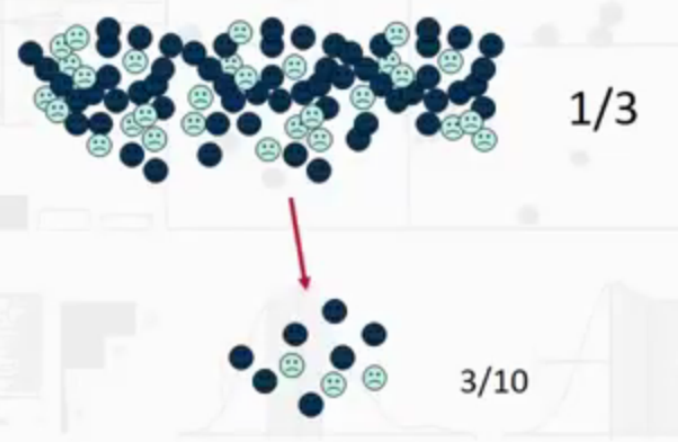
\includegraphics[scale=0.35]{ilu/bp.png}\end{center}\end{figure}
Dans la réalité, il est impossible de savoir si dans la population choisie précédemment, il y a réellement $\frac{1}{3}$ des détenus qui ont une symptomatologie depressive. La question que l'on peut se poser est dès lors que l'on réintègre l'échantillon de détenus et que l'on considère l'ensemble de la population, \textit{combien d'entre eux sont réellement dépressif}.\newline
On aurait tendance à répondre $30\%$; mais cela n'est vrai que si l'ensemble de la population est similaire à l'échantillon que l'on a extrait (que l'échantillon est dit représentatif) ce qui n'est pas forcément le cas.\newline
En effet, il existe, dans ce cas ci, une infinité de configurations possibles.
\begin{figure}[H]\begin{center}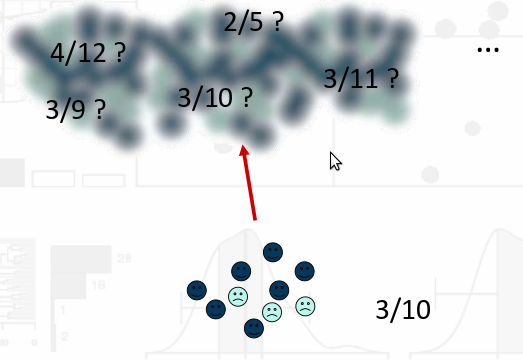
\includegraphics[scale=0.35]{ilu/bq.png}\end{center}\end{figure}
C'est à partir de ce moment que le calcul des probabilité va intervenir.\newline
\\
En effet, on peut montrer que si l'on part d'une population globale - Dans notre cas, la population des détenus masculins des prisons de France Métropolitaine - si l'on tire au sort un échantillon de $10$ sujets dont $3$ ont une symptomatologie depressive, alors on peut montrer qu'il y a \textbf{95 chances sur 100 que dans la population totale des détenus, la véritable proportion des détenus présentant cette caractéristiques sera comprise entre 8\% et 64\%}.\newline
On dit ainsi que l'intervalle $[8\%,64\%]$ est un intervalle de confiance à $95\%$ de la prévalence de la symptomatologie depressive.\newline
A ce stade, on peut considérer que l'intervalle est insuffisamment précis. Cela s'explique par la taille de l'échantillon (10 dans notre cas).\newline
\\
Imaginons alors que l'on tire au sort $100$ détenus, si $30\%$ sont déprimées alors il y a 95 chances sur 100 que la proportion de déprimés dans la population soit  comprise entre $21\%$ et $39\%$\newline
On dit ainsi que l'intervalle $[21\%,39\%]$ est un intervalle de confiance à $95\%$ de la prévalence de la symptomatologie depressive.\newline
\\
A nouveau, Imaginons alors que l'on tire au sort $1000$ détenus, si $30\%$ sont déprimées alors il y a 95 chances sur 100 que la proportion de déprimés dans la population soit  comprise entre $27\%$ et $33\%$\newline
On dit ainsi que l'intervalle $[27\%,33\%]$ est un intervalle de confiance à $95\%$ de la prévalence de la symptomatologie depressive.\newline
\\
\textbf{Note : } Plus la taille d'un échantillon est grande, plus l'intervalle de confiance sera précis.\newline
\\
\subsection{Méthode de calcul d'un intervalle de confiance}
En pratique, il s'agit d'un des derniers calculs que l'on va réaliser à la main lors d'une étude statistique.\newline
En effet, il existe une formule assez simple pour le déterminer.\newline
Si nous sommes intéressés par un paramètre et que ce dernier \underline{suit une distribution Normale}, que l'on dispose d'un échantillon tiré au sort dans une population et que l'on a estimé une valeur du paramètre, noté \textbf{m}, avec son écart-type, noté $\sigma$, alors \textbf{l'intervalle de confiance à 95\% du paramètre} est donné par : 
$$[m-1.96\times \sigma , m+1.96\times\sigma]$$
\textbf{Note : } Beaucoup de paramètres suivent une loi Normal, c'est notamment le cas de la moyenne et du pourcentage.\newline
\\
Un problème plus insidieux\footnote{Qui constitue un piège, qui cherche à tromper} est que l'échantillon doit être tiré au sort pour être réellement représentatif d'une distribution. Or dans beaucoup d'études, ces derniers ne le sont pas (Quand on interroge des individus avec un questionnaire, On ne tire pas ces derniers au sort, on va les rencontrer dans la rue, dans une classe ou sur internet).\newline
Quand un échantillon n'est pas tiré au sort, alors l'intervalle de confiance perd en signification. Stricto sensu, un IC (intervalle de confiance) est définit pour un échantillon construit aléatoirement. Quand l'échantillon n'est pas pris aléatoirement, certains diront l'on ne peut rien en conclure et d'autre préciseront que l'IC donne quand même une \textbf{idée} de la fluctuation ou de la valeur possible d'un paramètre dans une population plus grande (et non pas une valeur de confiance car l'échantillon n'a pas été tiré au sort).\newline
\\
Dans \textbf{R}, à l'aide de la librairie \textit{prettyR} et de la fonction \textbf{describe()}, il est possible d'estimer la moyenne et l'écart type de l'âge des détenus.
\begin{lstlisting}[language=html]
> smp <-read.csv2("/comptes/E131729J/XX_Université_fun/univfunR/TP/smp1.csv")
> library(prettyR)
> describe(smp$age)
> ##Application de la formule ci dessus
> borninf <- 38.9 - 1.96*(13.28/sqrt(797))
> borninf
[1] 37.97801
> bornsup <- 38.9 + 1.96*(13.28/sqrt(797))
> bornsup
[1] 39.82199
\end{lstlisting}
$$inf = \bar{x} - 1.96\times\frac{\sigma}{\sqrt{N}}\textrm{ et }sup = \bar{x} + 1.96\times\frac{\sigma}{\sqrt{N}}$$
On peut donc affirmer que sous réserve que la distribution suive une loi Normale, alors l'intervalle de confiance à 95\% de l'âge est obtenu par les valeurs.
$$[38,40] (\textrm{ans})$$
Voyons à présent comment estimmer un intervalle de confiance à 95\% pour un pourcentage.\newline Nous allons supposer avoir un échantillon de $10$ personnes. Dans ce dernier, nous avions observé 3 individus présentant une symptomatologie dépressive, tirés au sort dans une vaste population.\newline
Nous avions dis alors que l'intervalle de confiance à 95\% était à $[8\%,64\%]$.\newline
Pour estimer ces deux valeurs avec R, nous pouvons utiliser la librairie \textit{binom} et la fonction \textit{binom.confint()} avec pour paramètres la taille de l'échantillon prélevé, la population totale.
\begin{lstlisting}[language=html]
> library(binom)
> binom.confint(3,10,method="all")
          method x  n      mean      lower     upper
1  agresti-coull 3 10 0.3000000 0.10333842 0.6076747
2     asymptotic 3 10 0.3000000 0.01597423 0.5840258
3          bayes 3 10 0.3181818 0.07454423 0.5794516
4        cloglog 3 10 0.3000000 0.07113449 0.5778673
5          exact 3 10 0.3000000 0.06673951 0.6524529
6          logit 3 10 0.3000000 0.09976832 0.6236819
7         probit 3 10 0.3000000 0.08991347 0.6150429
8        profile 3 10 0.3000000 0.08470272 0.6065091
9            lrt 3 10 0.3000000 0.08458545 0.6065389
10     prop.test 3 10 0.3000000 0.08094782 0.6463293
11        wilson 3 10 0.3000000 0.10779127 0.6032219
\end{lstlisting}

Le problème de cette fonction est qu'il n'existe pas une mais plusieurs méthodes permettant de calculer des intervalles de confiance.\newline
Le statisticiens ne sont pas toujours d'accords sur la méthode à utiliser car en effet, certaines sont utiles pour des petits effectifs, d'autres plus puissantes, \dots \newline
On s'intéresse alors à la ligne suivante car on y retrouve les valeurs que nous avons calculé précédemment. 

\begin{lstlisting}[language=html]
> binom.confint(3,10,method="prop.test")
     method x  n mean      lower     upper
1 prop.test 3 10  0.3 0.08094782 0.6463293
\end{lstlisting}
En pratique, si l'on souhaite utiliser une méthode qui présente le moins le problèmes possibles, il faut choisir la méthode \textit{exact} dont les résultats obtenus sont très proches de nos résultats calculés : 
\begin{lstlisting}[language=html]
> binom.confint(3,10,method="exact")
  method x  n mean      lower     upper
1  exact 3 10  0.3 0.06673951 0.6524529
\end{lstlisting}
On peut considérer qu'il est un peu génant qu'il existe plusieurs méthodes permettant de calculer un intervalle de confiance et que toute ne parviennent pas aux mêmes résultats. \newline
Heureusement, quand la taille de l'échantillon est suffisamment grande, l'ensemble des méthodes convergent vers une même valeur. Reprenons notre exemple précédent, non plus sur 10 sujets mais sur 1000 et 300 symptômatologies observées : 
\begin{lstlisting}[language=html]
> binom.confint(300,1000,method="all")
          method   x    n      mean     lower     upper
1  agresti-coull 300 1000 0.3000000 0.2723966 0.3291341
2     asymptotic 300 1000 0.3000000 0.2715974 0.3284026
3          bayes 300 1000 0.3001998 0.2719448 0.3286787
4        cloglog 300 1000 0.3000000 0.2718595 0.3285966
5          exact 300 1000 0.3000000 0.2717211 0.3294617
6          logit 300 1000 0.3000000 0.2723865 0.3291466
7         probit 300 1000 0.3000000 0.2722277 0.3289871
8        profile 300 1000 0.3000000 0.2721340 0.3288893
9            lrt 300 1000 0.3000000 0.2721419 0.3289000
10     prop.test 300 1000 0.3000000 0.2719222 0.3296354
11        wilson 300 1000 0.3000000 0.2724068 0.3291239
\end{lstlisting}

Nous constatons alors que valeurs convergent toutes vers un l'intervalle de confiance : $$ [27\%,33\%]$$
\newpage
\section{Mesure de la force de liaison entre deux variables quantitatives : Le coefficient de corrélation}
Mesurer, quantifier, caractériser la force de l'association existante entre deux mesures est à la base de la plupart des expériences scientifiques. Ainsi, le physicien va t'il chercher à caractériser la relation qu'il observe entre la distance de chute d'un corps et sa vitesse. Le médecin, quant à lui, sera plus intéressé par la relation entre la tension artérielle et la probabilité d'apparition d'un infarctus.\newline
\\
\textit{Deux variables sont dites dépendantes quand la connaissance de l'un donne une indication sur la valeur de l'autre}. Le niveau d'indication peut être plus où moins élevé et cela correspond à des liaisons plus ou moins fortes.\newline
Il est possible de parler de \textbf{Force} d'une liaison. Prenons en exemple un couple de jumeaux : 
\begin{itemize}
\item Si vous connaissez la taille d'un des deux jumeaux, alors cela nous donne une indication assez précise sur la taille  du second jumeau. On dit alors que la relation est \textbf{forte}.
\item Si vous connaissez le revenu d'un des deux jumeaux, alors cela peux vous donner une indication statistique sur les revenus du second jumeau. Dans ce cas, la relation est \textbf{moins forte}.
\item Dans le cas où les deux jumeaux vont tous les deux jouer au casino, le niveau des pertes et des gains du premier jumeau sera une très maigre indication sur celles et ceux du second jumeau. On dira alors que la force de liaison est \textbf{très faible voire nulle}.
\end{itemize}
Un quiproquo très fréquent en statistique est celui qui est entre \textbf{la liaison et la causalité}. Ce n'est pas parce qu'il y a une liaison statistique que cela implique forcément une causalité entre deux variables (l'inverse est également faux).\newline
Il existe une liaison entre le fait d'avoir les dents jaunes et le fait d'attraper un cancer du poumons car les fumeurs ont souvent les dents jaunes et que fumer est un facteur de risque du cancer du poumon. Mais bien entendu, il n'y a aucune relation de cause à effet (causalité) entre avoir les dents jaunes et avoir un cancer du poumon.\newline
\\
Le grand classique pour quantifier la force de relation entre \textit{deux variables quantitatives} est le \textbf{coefficient de corrélation de PEARSON} (Mais il y a mieux). Il faut avoir à l'esprit que la corrélation de PEARSON est un cas particulier de liaison, liaison que l'on qualifie souvent de monotone ou de linéaire :
\begin{center}
\textit{Soit X et Y, deux variables. Plus l'une est grande, plus l'autre le sera également.}
\end{center}  
Le coefficient de corrélation est souvent désigner par la lettre \textbf{r} et ce dernier \textit{varie entre $\pm 1$}. Quand $r=0$, de façon un peu hâtive, on considère que les deux variables sous jacentes sont indépendantes; Malheureusement ce n'est pas l'interprétation qu'il faut lui donner. \newline 
Il est vrai que dans le cas où les deux variables suivent une loi Normale, il peut arriver que si l'une des deux variables ne suit pas réellement une loi Normale que $r$ soit égal à 0 et pourtant, il y a bien une relation entre les deux variables (cas rare). \newline
Quand $r=\pm 1$, la force de la liaison est tellement importante que la connaissance d'une variable donne exactement la valeur de l'autre variable. On dit alors que les deux variables sont \textbf{mutuellement déterminée} au moyen d'une relation linéaire du type :
$$Y=a\times X + b$$
Quand $r>0$, plus l'une des variables est grande, plus l'autre le sera également alors que quand $r<0$, quand une variable augmente, l'autre diminue. Par exemple, entre 0 et 6 ans, il y a une corrélation positive assez forte entre la taille et l'âge; En effet, plus l'enfant vieilli, plus il sera grand. Au contraire, à partir de 60 ans, il y a une corrélation légère mais négative entre l'âge et la taille à cause de l'ostéoporose, plus on vieilli, plus on se tasse.\newline
\\
L'expression mathématique qui permet de traduire une corrélation n'est pas si compliquée que ça : 
$$r=\frac{(x_{1}\cdot y_{1} + \dots + x_{n}\cdot y_{n})-n\times\bar{x}\times\bar{y}}{(n-1)\times \sigma(x)\times \sigma(y)}$$
Cette formule correspond à la covariance divisée par la racine carré des variances.\newline 
Nous avons vu précédemment que la variance n'était pas facile à interpréter et naturellement, il se pose la question de l'interprétation de la taille et de l'importance de la valeur d'un coefficient de corrélation.
\begin{center}
\begin{tabular}{|c|c|c|}\hline

\textbf{Corrélation} &  	\textbf{Négative} &  	\textbf{Positive} \\\hline
\textbf{Faible} 	& de -0,5 à 0,0 	& de 0,0 à 0,5 \\\hline
\textbf{Forte} &	de -1,0 à -0,5 &	de 0,5 à 1,0\\
\hline
\end{tabular}
\end{center}
Dans certains livres, il est dit que le pourcentage de variance partagé entre deux variables est égal au carré du coefficient de corrélation. Cette assertion est mathématiquement vraie mais quel en est vraiment le sens. Soient x et y, deux variables qui corrèlent à 0,6, le pourcentage de variance partagé est donc de 0,36 soit 36\%. Cela ne signifie pas que les variables se ressemble seulement à 36 \%.\newline
Un façon d'interpréter ce qu'est une corrélation de $0,6$ ou de $0,4$ est de réaliser des simulation et d'analyser des graphiques en $(O,x,y)$.

\begin{figure}[H]\begin{center}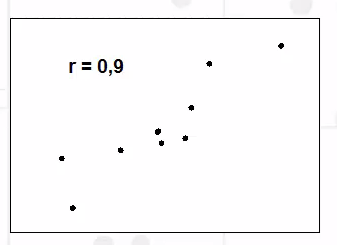
\includegraphics[scale=0.4]{ilu/br.png}\caption{Représentation graphique d'une corrélation à r=0,9 entre deux variables pour 10 individus}\end{center}\end{figure}
\begin{figure}[H]\begin{center}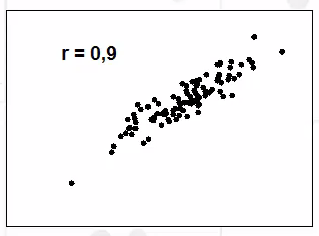
\includegraphics[scale=0.4]{ilu/bu.png}\caption{Représentation graphique d'une corrélation à r=0,9 entre deux variables pour 100 individus}\end{center}\end{figure}
\begin{figure}[H]\begin{center}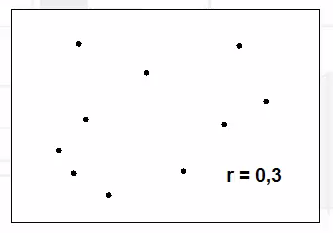
\includegraphics[scale=0.4]{ilu/bs.png}\caption{Représentation graphique d'une corrélation à r=0,3 entre deux variables pour 10 individus}\end{center}\end{figure}
\begin{figure}[H]\begin{center}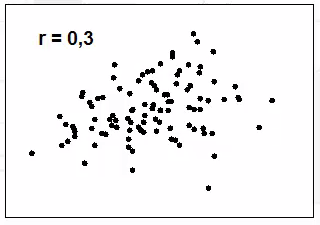
\includegraphics[scale=0.4]{ilu/bv.png}\caption{Représentation graphique d'une corrélation à r=0,3 entre deux variables pour 100 individus}\end{center}\end{figure}
\begin{figure}[H]\begin{center}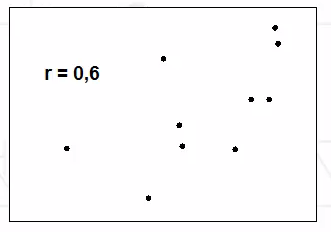
\includegraphics[scale=0.4]{ilu/bt.png}\caption{Représentation graphique d'une corrélation à r=0,6 entre deux variables pour 10 individus}\end{center}\end{figure}
\begin{figure}[H]\begin{center}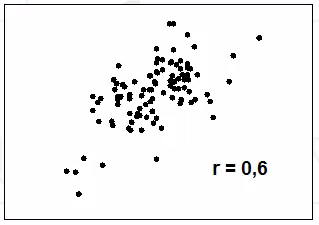
\includegraphics[scale=0.4]{ilu/bw.png}\caption{Représentation graphique d'une corrélation à r=0,6 entre deux variables pour 100 individus}\end{center}\end{figure}
On voit que pour $r=0.9$, l'association entre $x$ et $y$ est évidente alors que pour $r=0.3$ et à l'oeil nu, il est difficile d'affirmer que dès lors que 
$x$ est grand, $y$ l'est aussi.\newline
\\
Nous allons voir comment calculer avec \textbf{R}, un coefficient de coefficient de PEARSON. Dans l'étude sur la santé mentale en prison, nous allons calculer le coefficient de corrélation entre l'âge et le nombre d'enfant.
\begin{lstlisting}[language=html]
> setwd("~/Desktop/DIVERS + TEMPLATES/R/TP")
> smp.c <- read.csv2("/Users/mehdilatif/Desktop/DIVERS + TEMPLATES/R/TP/smp2.csv")
> table(smp.c$age)
19 20 21 22 23 24 25 26 27 28 29 30 31 32 33 34 35 36 37 38 39 40 41 42 43 44 
45 46 47 48 49 50 51 52 53 54 55 15 15 18 13 23 30 22 30 25 21 20 25 18 22 26 
20 16 18 25 24 23 22 23 19 17 19 17 16 12 17 23 16 11 10  8 11  6 56 57 58 59 
60 61 62 63 64 65 66 67 68 69 70 71 72 73 74 77 79 81 83 14  9  7  6  7  5  7  
4  5  3  6  4  2  1  1  6  3  2  2  3  1  1  2 

> table(smp.c$n.enfant)
  0   1   2   3   4   5   6   7   8   9  10  11  13 
214 220 125 101  55  31   7   7   7   2   2   1   1 
> plot(jitter(smp.c$age),jitter(smp.c$n.enfant))
\end{lstlisting}

\begin{figure}[H]\begin{center}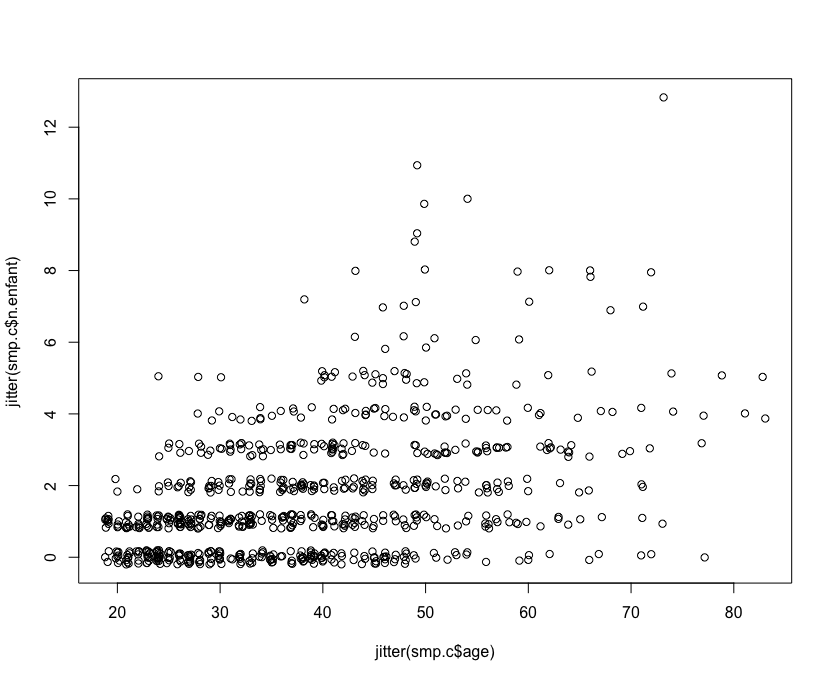
\includegraphics[scale=0.5]{ilu/bx.png}\end{center}\end{figure}

La fonction qui permet de calculer un coefficient de corrélation de PEARSON sous \textbf{R} est la suivante :\newline
\textbf{Attention : } Ne pas oublier le paramètre \textit{use="complete.obs"} qui permet de gérer les données manquantes.
\begin{lstlisting}[language=html]
> cor(smp.c$age,smp.c$n.enfant,use="complete.obs")
[1] 0.4326039
\end{lstlisting}
Il est important de garder à l'esprit que le coefficient de corrélation ne répond pas à toute les questions concernant la quantification des relations entre deux variables quantitatives. Non seulement deux variables peuvent être liées alors que leurs corrélation est nulle (cas des relation quadratique entre deux variables).\newline
Il existe également des situations où la forme de la liaison entre $x$ et $y$ qui intéresse les expérimentateurs ne correspond pas à la corrélation de PEARSON. C'est notamment le cas lorsque l'on s'intéresse à la \textbf{concordance} entre deux variables aléatoires\footnote{L'accord observé entre des jugements qualitatifs ou non, résulte de la somme d'une composante «aléatoire» et d'une composante d'accord «véritable».Le coefficient Kappa $K$ propose de chiffrer l'intensité ou la qualité de l'accord réel entre des jugements qualitatifs appariés.Il exprime une différence relative entre la proportion d'accord observée $P_{0}$ et la proportion d'accord aléatoire $P_{e}$ qui est la valeur espérée sous l'hypothèse nulle d'indépendance des jugements, divisée par la quantité disponible au-delà de l'accord aléatoire. En définitive, K est un pourcentage de l'accord maximum corrigé de ce qu'il serait sous le simple effet du hasard. La valeur vraie du coefficient Kappa dans la population est une variable aléatoire qui suit approximativement une loi de Gauss de moyenne $K$ et de variance $Var(K)$. L'hypothèse nulle $H_{0}$ est K = 0 contre l'hypothèse alternative $H_{1}$ : $K > 0$. Dans le cas d'une étude d'accord entre deux observateurs statistiquement indépendants ayant r modalités de jugement, avec $r^{3}2$, le coefficient Kappa s'écrit : $\frac{P_{0}-P_{e}}{1-P_{e}}$ avec $P_{0}$ : la proportion d'accord observée et $P_{e}$ : la proportion d'accord aléatoire ou concordance attendue sous l'hypothèse d'indépendance des jugement.}. 
Ou alors, deux biologistes qui tentent de calibrer un appareil, un nouvel appareil qui ne coûte pas très cher au moyen d'un autre appareil qui lui est une référence parce qu'il coûte très cher. Dans ce type de situation, si le nouvel appareil dit systématiquement un résultat deux fois moins important que l'appareil de référence, alors la corrélation sera parfaite, elle vaudra $1$ et pourtant le nouvel appareil sera bien mauvais puisque systématiquement il donne un résultat faux.

\newpage 
\section{Risque relatif et odds-ratio}
Dans ne nombreuses disciplines, nous sommes amenés à nous intéresser à la  quantification de la force de liaison entre deux variables binaires. le genre et le fait d'être oui ou non au chômage. En médecine, un cas très fréquent est celui de l'association entre une maladie et un facteur de risque, par exemple celui d'être fumeur et de développer plus tard un infarctus du myocarde ou plus généralement une pathologie coronarienne.\newline
Pour entrer deans le détail, nous allons considérer le cas particulier de la relation entre une maladie et un facteur de risque. Les données peuvent être représentées au moyen d'un tableau comme celui ci dessous : 

\begin{center}
\begin{tabular}{l|l|l|ll}
\cline{2-3}
 & \multicolumn{2}{l|}{\textbf{Maladie}} &  &  \\ \cline{2-3}
 & \textit{Oui} & \textit{Non} &  &  \\ \cline{1-3}
\multicolumn{1}{|l|}{\textbf{FR = "Oui"}} & a & b &  &  \\ \cline{1-3}
\multicolumn{1}{|l|}{\textbf{FR = "Non"}} & c & d &  &  \\  \cline{1-3}
\end{tabular}
\end{center}
On y représente en colonne les individus malades (\textit{oui}) et non malades (\textit{non}) et en ligne, les sujets ayant un facteur de risque (\textit{FR="Oui"}) et ceux qui n'en ont pas (\textit{FR="Non"}).\newline
Le paramètre le plus intuitif pour quantifier la force de l'association entre cette maladie et ce facteur de risque  est le \textbf{Risque Relatif (RR)} qui représente le pourcentage de sujets malades parmi ceux qui ont un facteur de risque divisé par le pourcentage de sujets malades chez ceux qui ne sont pas porteurs du facteur de risque : 
$$\mathbf{\textrm{RR}} = \frac{\frac{a}{a+b}}{\frac{c}{c+d}}$$
Nous avons là un paramètre simple et facile à interpréter.\newline
\\
Le risque relatif n'est pas le seul paramètre que l'on peut utiliser dans cette situation. Il existe aussi l'\textbf{Odds-ratio}. Ce dernier est parfois traduit par \textit{Rapport des cotes} (au sens valeur \dots coté en bourse).\newline
Il se calcul comme le rapport entre le rapport des individus malades sur ceux qui ne le sont pas, sachant que les deux ont un facteur de risque, sur le rapport des individus malade sur ceux qui ne le sont pas sachant qu'ils n'ont pas de facteur de risque : 
$$\mathbf{\textrm{OR}} = \frac{\frac{a}{b}}{\frac{c}{d}}$$
A l'évidence, l'Odds-ratio est moins intuitif que le Risque Relatif.
\subsection{Odds-ratio VS Risque Relatif}
L'Odds-ratio a un inconvénient évident, on ne sait pas trop ce qu'il mesure au contraire du risque relatif qui lui a un sens clair et précis que tout le monde appréhende facilement.\newline
\\
Cependant, L'Odds-ratio présente de nombreux avantages.\newline
En effet, il permet la gestion des facteurs de confusion. Imaginons que nous souhaitions mettre en évidence un association entre obésité et infarctus du myocarde. Il suffit de montrer qu'il y a une relation (association) statistiquement significative mais nous avons du mal à l'interpréter car il est possible que ce ne soit pas l'obésité en elle même qui soit associée à l'infarctus du myocarde mais peut être que cette dernière est associée à une faible pratique du sport et que c'est l'absence de pratique du sport qui génère ce risque d'infarctus du myocarde.\newline
Pour répondre à cette question de santé publique, une solution possible est d'utiliser un modèle statistique qui va permettre de trouver le poids spécifique de l'obésité et de la pratique du sport sur la survenue de l'infarctus du myocarde(Régression logistique, très utile pour déterminer des relations complexes entre es variables "binaires"). Ces modèles permettent assez facilement d'estimer des Odds-ratios ajustés et beaucoup plus difficilement des Risques Relatifs ajustés. 
D'où la recherche de l'Odds-ratio qui peut être généraliser au cas de la recherche de facteurs de confusion.\newline
\\
De plus, l'Odds-ratio peut être utilisé dans les enquêtes dites \textit{cas-témoin}\footnote{Étude statistique observationnelle rétrospective utilisée en épidémiologie. Les études cas-témoins sont utilisées pour mettre en évidence des facteurs qui peuvent contribuer à l'apparition d'une maladie en comparant des sujets qui ont cette maladie (les cas) avec des sujets qui n'ont pas la maladie mais qui sont similaires par ailleurs (les témoins).} Pour évaluer un Odds-ratio ou un Risque Relatif, par exemple pour déterminer la relation entre l'obésité et le risque d'infarctus du myocarde, on peut réaliser une enquête en population générale c'est à dire tirer au sort un nombre suffisamment grand de personnes (1000 voir 10000) dans la population générale et leurs demander si ils ont déjà eu un infarctus du myocarde et également regarder si ils sont obèse ou non.\newline
On réaliser alors le tableau suivant : 
\begin{center}
\begin{tabular}{l|l|l|ll}
\cline{2-3}
 & \multicolumn{2}{l|}{\textbf{Infarctus du myocarde}} &  &  \\ \cline{2-3}
 & \textit{Oui} & \textit{Non} &  &  \\ \cline{1-3}
\multicolumn{1}{|l|}{\textbf{Obèse = "Oui"}} & a & b &  &  \\ \cline{1-3}
\multicolumn{1}{|l|}{\textbf{Obèse = "Non"}} & c & d &  &  \\  \cline{1-3} 
\end{tabular}
\end{center}
On peut donc calculer les Risques Relatif et le Odds-ratio correspondants à cette étude.\newline
Mais pour pouvoir calculer ces paramètres avec suffisamment de précision et compte tenu de la rareté de l'infarctus du myocarde, il va falloir inclure dans l'étude un grand nombre de sujet et il est possible que 1000 ou 10000 sujets ne soient pas suffisants.\newline
Ce type d'étude va donc vite devenir très onéreux. \newline
Un façon de réaliser ce type d'étude à bas coût est de réaliser cette étude sur $X$ sujets sains et $X$ sujets atteints d'un infarctus du myocarde. C'est ce que l'on appelle une étude de cas-témoins. Dans le cadre de ces études, une centaine de cas et de témoins peuvent suffire.\newline
La question est maintenant de savoir si le calcul d'un Risque Relatif ou d'un Odds-ratio est possible à partir ce type d'enquête.\newline
Il s'avère que la réponse est \textbf{Non avec un Risque Relatif } et \textbf{Oui avec un Odds-ratio}.\newline
\\
Enfin, l'argument conclusif est que certes, l'Odds-ratio est difficilement interprétable mais quand le facteur étudié (dans notre cas, l'infarctus du myocarde) est suffisamment rare, c'est à dire que sa prévalence est inférieure à 5\%, alors l'Odds-ratio tend à être équivalent au Risque Relatif.\newline
\\ 
Nous pouvons nous interroger légitiment sur le fait que \textit{l'Odds-ratio puisse être estimé à la fois dans une enquête cas-témoins et dans une enquête en population générale}\footnote{Population générale : témoins tirés au sort sur listes électorales, liste téléphonique (random digit dialing)\dots Epidémiologie de population (population générale) - Descriptif : Répartition et fréquence d'une maladie - Analytique : Recherche de facteurs de risque - Evaluatif : Evaluation d'action de santé publique (action de prévention, de dépistage \dots)} alors que \textit{le Risque Relatif ne peut être calculé que dans le cadre d'une enquête en population générale}.\newline
\\
Pour en être convaincu, analysons l'exemple suivant où nous allons chercher une relation entre le fait de fumer et d'être enrhumé  :

\begin{center}
\begin{tabular}{l|l|l|ll}
\cline{2-3}
 & \multicolumn{2}{l|}{\textbf{Rhume}} &  &  \\ \cline{2-3}
 & \textit{Oui} & \textit{Non} &  &  \\ \cline{1-3}
\multicolumn{1}{|l|}{\textbf{Tabac = "Oui"}} & 30 & 300 &  &  \\ \cline{1-3}
\multicolumn{1}{|l|}{\textbf{Tabac = "Non"}} & 30 & 600 &  &  \\  \cline{1-3}
\end{tabular}
\end{center}
Dans cette étude, nous avons simulé une enquête auprès de 1000 sujets.
$$\mathbf{\textrm{RR}} = \frac{\frac{30}{300+30}}{\frac{30}{600+30}} = 1,91$$
$$\mathbf{\textrm{OR}} = \frac{\frac{30}{300}}{\frac{30}{600}}=2$$.

On constate, comme c'est généralement le cas, que l'\textbf{Odds-ration surestime le Risque relatif}.\newline  
\\
Imaginons maintenant que l'on réalise une enquête cas-témoins où nous allons étudier 90 personnes non enrhumées, 60 personnes enrhumées avec, pour chacun, un niveau d'exposition au tabac exactement similaire à celui de l'étude que l'on a réalisé précédemment :
\begin{center}
\begin{tabular}{l|l|l|ll}
\cline{2-3}
 & \multicolumn{2}{l|}{\textbf{Rhume}} &  &  \\ \cline{2-3}
 & \textit{Oui} & \textit{Non} &  &  \\ \cline{1-3}
\multicolumn{1}{|l|}{\textbf{Tabac = "Oui"}} & 30 & 30 &  &  \\ \cline{1-3}
\multicolumn{1}{|l|}{\textbf{Tabac = "Non"}} & 30 & 60 &  &  \\ \cline{1-3}
\end{tabular}
\end{center}

$$\mathbf{\textrm{RR}} = \frac{\frac{30}{30+30}}{\frac{30}{60+30}} = 1,5$$
$$\mathbf{\textrm{OR}} = \frac{\frac{30}{30}}{\frac{30}{60}}=2$$.
Nous avons dès lors, un Risque Relatif de 1.5, inférieur à celui de la première étude alors que l'Odds-ratio est toujours égal à 2.\newline
On peut donc en déduire que l'Odds-ration est plus stable que le Risque Relatif.\newline
\\
Passons maintenant à un cas concret : Nous allons essayer de déterminer dans quelle mesure un niveau élevé d'évitement du danger est associé à un trouble dépressif.\newline
Dès lors, nous rencontrons un premier problème. En effet, la variable évitement du danger (\textit{ed}) est codée en trois classe : 
\begin{enumerate}
\item Faible 
\item Modérée 
\item Elevée
\end{enumerate}
Il faut donc la redéfinir en variable binaire que nous allons appeler \textit{ed.bin} ou les valeurs 1 (Faible) et 2 (Modérée) seront codées en 0 et 3 (Elevée) sera codée en 1.
\begin{lstlisting}[language=html]
> smp <-read.csv2("/comptes/E131729J/XX_Université_fun/univfunR/TP/smp1.csv")
> setwd("~/XX_Université_fun/univfunR/TP")

> ##variable de mesure d'évitement du danger avant encodage binaire

> table(smp$ed,useNA = "always")
   1    2    3 <NA> 
 315  155  222  107 

> ##variable de mesure d'évitement du danger après encodage binaire

> ### SI la valeur de ed est supérieure stricte à 2 (=3 -> forte), alors smp$ed.bin[i] = 1, sinon smp$ed.bin[i]=0

> smp$ed.bin <- ifelse(smp$ed>2,1,0)

> table(smp$ed.bin,useNA = "always")

   0    1 <NA> 
 470  222  107 

> ##Analyse à l'oeil nu des valeurs avant et apès modification

> str(smp)
'data.frame':	799 obs. of  10 variables:
 $ age      : int  31 49 50 47 23 34 24 52 42 45 ...
 $ prof     : Factor w/ 8 levels "agriculteur",..: 3 NA 7 6 8 6 3 2 6 6 ...
 $ dep.cons : int  0 0 0 0 1 0 1 0 1 0 ...
 $ scz.cons : int  0 0 0 0 0 0 0 0 0 0 ...
 $ grav.cons: int  1 2 2 1 2 1 5 1 5 5 ...
 $ n.enfant : int  2 7 2 0 1 3 5 2 1 2 ...
 $ rs       : int  2 2 2 2 2 1 3 2 3 2 ...
 $ ed       : int  1 2 3 2 2 2 3 2 3 2 ...
 $ dr       : int  1 1 2 2 2 1 2 2 1 2 ...
 $ ed.bin   : num  0 0 1 0 0 0 1 0 1 0 ...

> ##Analyse croisée de ed.bin par rapport à ed grâce à la fonction table :

> table(smp$ed.bin,smp$ed,useNA = "always")      
         1   2   3 <NA>
  0    315 155   0    0
  1      0   0 222    0
  <NA>   0   0   0  107
  
> ###Ajout du nom des variables

> table(smp$ed.bin,smp$ed,deparse.level = 2,useNA = "always")
          smp$ed
smp$ed.bin   1   2   3 <NA>
      0    315 155   0    0
      1      0   0 222    0
      <NA>   0   0   0  107
\end{lstlisting}

Pour \textit{ed = 1} et \textit{ed = 2} nous obtenons \textit{ed.bin = 0} et pour \textit{ed = 3}, nous avons bien \textit{ed.bin = 1}.\newline

\begin{figure}[H]\begin{center}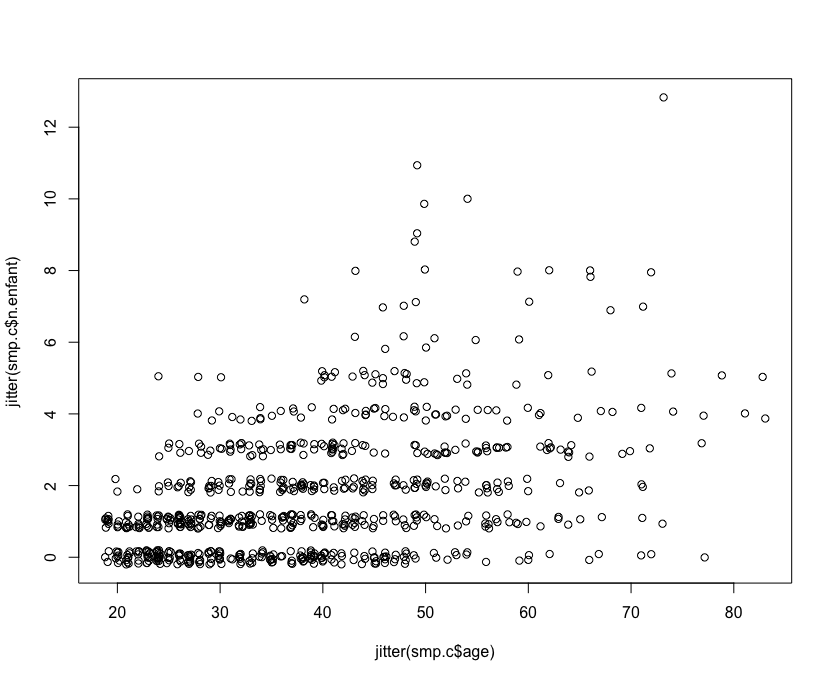
\includegraphics[scale=0.5]{ilu/bx.png}\end{center}\end{figure}
Calculons maintenant l'Odds-Ration et le Risque relatif pour établir une relation entre l'évitement du danger et la symptomatologie dépressive. Nous allons devoir faire appel à la libraire \textit{Epi} et utiliser la fonction \textit{twoby2()}.\newline
\textbf{Attention : } Il nous faut modifier les paramètres de la fonction \textit{twoby2()} et lui passer \textit{1-ed.bin} et {1-dep.cons}. Cette variation vient du fait que par défaut, la fonction \textit{twoby2()} considère que lorsqu'une variable est codée en binaire :
\begin{itemize}
\item 0 signifie que l'on est malade et 1 signifie que l'on est pas malade
\item 0 signifie que l'on a le facteur de risque et 1, que l'on ne possède pas le facteur de risque. 
\end{itemize} 
Alors que dans notre jeu de données, c'est exactement l'inverse.
\begin{lstlisting}[language=html]
> twoby2(1-smp$ed.bin,1-smp$dep.cons)
2 by 2 table analysis: 
------------------------------------------------------ 
Outcome   : 0 
Comparing : 0 vs. 1 

    0   1    P(0) 95% conf. interval
0 126  96  0.5676    0.5016   0.6312
1 135 335  0.2872    0.2481   0.3298

                                   95% conf. interval
             Relative Risk: 1.9760    1.6456   2.3726
         Sample Odds Ratio: 3.2569    2.3361   4.5408
Conditional MLE Odds Ratio: 3.2508    2.3037   4.6035
    Probability difference: 0.2803    0.2020   0.3549

             Exact P-value: 0 
        Asymptotic P-value: 0 
------------------------------------------------------
\end{lstlisting}
On obtient donc un Risque Relatif à 1.97 et un Odds-Ratio à 3.26. \newline
Dans ce cas, l'Odds-Ratio est "assez sensiblement" différent du risque relatif car nous sommes dans une situation où la prévalence de la maladie n'est pas faible. En effet, dans notre étude, entre 30 et 40\% des détenus présentent un symptomatologie dépressive. Nous ne sommes donc pas de la cas d'une pathologie rare (comme dans notre étude de l'infarctus du myocarde) et donc l'Odds-Ratio est très difficilement interprétable.\newline
Il nous faudra alors nous focaliser sur le Risque Relatif  $\simeq$ 2.\newline 
\textbf{On peut donc en déduire que l'on a deux fois plus de risque de présenter un état dépressif lorsque l'on a un niveau d'évitement du danger élevé par rapport au contraire}.
\newpage 
\section{Tests statistiques : le "p" }
Dans les sciences de la vie, les sciences humaines et sociales, lorsque l'on fait une découverte, il faut d'abord s'assurer qu'elle n'est pas dû au hasard. \newline
C'est à cela que servent les \textbf{tests statistiques}.\newline
\\
Les tests statistiques sont souvent considérés comme un domaine un peu basique de la science statistique mais en réalité, ce sont des techniques qui sont très délicates à comprendre.\newline
Nous allons commencer simplement par \textbf{le test du p} ou \textbf{p-value} que l'on retrouve dans de nombreuses publications scientifiques.\newline
\\
Dans le chapitre précédent, nous avons calculé la corrélation entre l'âge des détenus et leurs nombres d'enfants : 
\begin{lstlisting}[language=html]
> smp <-read.csv2("/comptes/E131729J/XX_Université_fun/univfunR/TP/smp1.csv")
> setwd("~/XX_Université_fun/univfunR/TP")
> str(smp)
'data.frame':	799 obs. of  9 variables:
 $ age      : int  31 49 50 47 23 34 24 52 42 45 ...
 $ prof     : Factor w/ 8 levels "agriculteur",..: 3 NA 7 6 8 6 3 2 6 6 ...
 $ dep.cons : int  0 0 0 0 1 0 1 0 1 0 ...
 $ scz.cons : int  0 0 0 0 0 0 0 0 0 0 ...
 $ grav.cons: int  1 2 2 1 2 1 5 1 5 5 ...
 $ n.enfant : int  2 7 2 0 1 3 5 2 1 2 ...
 $ rs       : int  2 2 2 2 2 1 3 2 3 2 ...
 $ ed       : int  1 2 3 2 2 2 3 2 3 2 ...
 $ dr       : int  1 1 2 2 2 1 2 2 1 2 ...
> cor(smp$age,smp$n.enfant,use="complete.obs")
[1] 0.4326039
\end{lstlisting}
Cette corrélation vaut $0.4$, elle est positive et substantielle\footnote{Qui est important}.\newline
\\
Cependant, on peut se demander dans quelle mesure le hasard pourrait expliquer à lui tout seul une telle corrélation. En effet, si nous prenons n'importe quelle paire de variable, il se peut que par hasard, la corrélation entre ces deux variables soit non nulle.\newline
Voyons cela sur un autre exemple : \textit{Prenons 2 dés, un dans chaque mains et lancés ces derniers 10 fois}. On peut obtenir les résultats suivants (avec des résultats de mesures quantitatives comprises entre 1 et 6).
\begin{center}
\begin{tabular}{|c|c|c|c|c|c|c|c|c|c|c|}
\hline
\textbf{MG} & 3 & 3 & 6 & 5 & 1 & 4 & 1 & 6 & 5 & 5 \\ \hline
\textbf{MD} & 4 & 5 & 2 & 3 & 5 & 4 & 5 & 5 & 4 & 4 \\ \hline
\end{tabular}
\end{center}
Il est possible de calculer un coefficient de corrélation entre les variables \textbf{MG} (Main Gauche) et \textbf{MD} (Main Droite). Ici, par construction, on sait qu'il n'existe pas de corrélation entre ces deux résultats.\newline
Néanmoins, à partir des données présentées ci dessus, on obtient une corrélation \textbf{r=-0.6}.\newline
Cela signifie qu'en pratique, si l'on réalise une experience mesurant deux variables quantitatives \underline{totalement indépendantes} sur 10 sujets, on peut très bien obtenir par le simple effet du hasard, un coefficient de corrélation non nul et aussi important que $|r|=0.6$\newline 
\\
Cette part de hasard dans les résultats de cette expérience peut avoir peut avoir des conséquences très gênantes quand on fait de la recherche.\newline
En effet, si nous nous trouvons dans le cadre d'un essai thérapeutique et que l'on compare les effets d'un médicament A à un médicament B. Après tirage au sort et protocole en double aveugle\footnote{L'étude randomisée en double aveugle, avec répartition aléatoire est une démarche expérimentale utilisée dans de nombreuses disciplines de recherche tels la médecine, les sciences sociales et la psychologie,\dots. En pharmacie, elle est utilisée dans le développement de nouveaux médicaments, et pour évaluer l'efficacité d'une démarche, d'un traitement.} réalisé dans des circonstances optimales, nous obtenons la guérison de 40 \% dans le groupe ayant pris le médicament A et de 30\% dans celui qui a pris le médicament B, La question que l'on peut se poser est : Dans quelle mesure puis je dire que la différence observée entre les deux traitements provient bien d'une différence d'efficacité et non d'un simple effet aléatoire provenant de la randomisation\footnote{Méthode de répartition fondée sur le hasard.La randomisation est une méthode qui permet d'introduire un élément aléatoire dans une étude.} entre les deux groupes.\newline
\\
Revenons plus précisément sur cet exemple : il s'agit d'un essai thérapeutique randomisé (c'est à dire que l'on a tiré au sort l'attribution du médicament A ou du médicament B pour chaque patients). \newline
100 patients ont reçu le médicament A et 100 patients ont reçus le médicament B; 40 patients sur 100 (40\%) ont guéri avec A et 30 patients avec B (30\%). A l'évidence, \textit{A est plus efficace que B}.\newline
Néanmoins, on peut se poser la question suivante : \textit{Est ce que le différentiel d'efficacité de 10\% est significatif ou est il compatible avec les inévitables fluctuations issues du tirage au sort ?}\newline
\\
Pour répondre à cette question, nous allons tenter de la reformuler en la formalisant davantage : \newline
Imaginons que A et B soit d'une efficacité équivalente, Quelle est l'estimation la plus probable de l'efficacité de A (ici, égale à l'efficacité de B) ?\newline 
Comme A et B ont la même efficacité, on peut mélanger le groupe ayant reçu le traitement A avec celui ayant reçu le médicament B. En mélangeant ces deux groupes, le taux de guérison est la moyenne des taux de guérison individuel de chaque groupe c'est à dire 35\%.\newline
Nous avons donc un population de patients éligibles qui peuvent recevoir les traitements A ou B et l'efficacité de A est égale à celle de B. On peut en déduire que l'efficacité du traitement que va recevoir chaque patient est de 35\%.\newline
Si partant de cette population, on sélectionne 100 patients qui vont recevoir A et 100 patients qui vont recevoir B, quelle est l'estimation la plus probable du taux de guérison avec chaque médicaments ?\newline
Si tout se passe dans l'idéal, alors 35 patients vont guérir avec A et 35 patients avec B. Cependant, en pratique, il est tout a fait possible que cela ne se passe pas comme ça ; Il est possible que 36 personnes guérissent avec A et 37 avec B. Il est même possible que 40 personnes guérissent avec A et 30 avec B \dots La question que l'on doit se poser à ce stade de l'expérimentation est : \textit{Dans quelle mesure la différence de 10\% que nous avons observée entre l'efficacité dans le groupe A et l'efficacité dans le groupe B est elle compatible avec un tirage au sort réalisé dans une population où 35\% des sujets vont guérir ?}\newline
\\
Nous avons là exactement la définition de \textbf{p} à savoir, la probabilité que le hasard puisse expliquer à lui seul une différence d'efficacité au moins aussi importante que celle que l'on a observé. 
$$p = P\left((|\textrm{Guérison}_{A_{\%}} - \textrm{ Guérison}_{B_{\%}}|>10\%)\|\textrm{Guérison}_{Globale_{\%}} = 35\%\right)$$
Il est possible de calculer cette probabilité et dans le cas qui nous intéresse, on trouve $p=0,14$.\newline
Il y a donc 14\% de chance que le hasard puisse expliquer à lui seul que 40\% des sujets ont guéris avec A et 30\% avec B ou d'une différence encore plus importante d'efficacité.\newline
En pratique, 14\% c'est trop. On va donc considérer que la différence d'efficacité entre les deux medicaments n'est pas significative. La règle tacite communément admise est de considérer que si la probabilité de p avait été inférieur à 5\%, alors il aurait été possible de dire que la différence d'efficacité est statistique significative. 
\subsubsection*{Introduction de la valeur-p par Ronald Fisher}
Le statisticien Ronald Fisher a introduit les termes de significativité, d'hypothèse nulle, et l'utilisation de la valeur-p. Il rejetait toutefois la notion de puissance statistique : selon lui, l'hypothèse nulle ne peut jamais être acceptée, mais peut seulement être rejetée par le test statistique. Dans cette approche, la valeur-p est considérée comme une mesure d'à quel point les données plaident contre l'hypothèse nulle. Les seuils suivants sont généralement pris pour référence :
\begin{itemize}
\item   $p\leq 0.01$ : très forte présomption contre l'hypothèse nulle
\item $ 0.01<p\leq 0.05$ : forte présomption contre l'hypothèse nulle
\item $0.05<p\leq 0.1$ : faible présomption contre l'hypothèse nulle
\item $ p>0.1$ : pas de présomption contre l'hypothèse nulle
\end{itemize}
Pour un différentiel d'efficacité constant, la valeur de \textbf{p} dépend très fortement de la taille des groupes comparés. En effet, dans les même exemple : 
\begin{itemize}
\item Pour 100 sujets par groupe, $p=0.14$
\item Pour 200 sujets par groupe, $p=0.036$
\item Pour 1000 sujets par groupe, $p=0.000003$
\end{itemize}
Nous voyons ainsi qu'avec de grands échantillons, l'influence possible du hasard diminue considérablement.
\newpage
\section{L'approche de Neyman et Pearson :}
Nous avons vu dans le chapitre précédent le principe du test du p-value. Il faut d'ailleurs constater que dans la réalité des travaux scientifiques, les tests statistiques se résument à une succession de test du p-value.\newline
Cependant, dans le cadre scolaire, on apprend à utiliser les tests statistiques et non le p-value. L'un des principes des tests statistiques est celle de la théorie des tests d'hypothèses de \textbf{NEYMAN \& PEARSON}.\newline
\\
Les test d'hypothèses selon la théorie de NEYMAN \& PEARSON reposent sur une formulation assez formelle ; De manière assez simpliste, nous allons considérer que nous devons choisir entre les des deux hypothèse suivantes : $H_{0}$ et $H_{1}$.\newline
Soient deux évènements $A$ et $B$.\newline
$H_{0}$ représente en générale le \textit{statu quo} (ou profil bas) pour lequel :
$$P(A)=P(B)$$
$H_{1}$ représente, quant à lui, le but de l'expérience pour lequel :
$$P(A)\neq P(B)$$
C'est l'hypothèse $H_{1}$ que le scientifique souhaite démontrer.\newline 
Dans le cadre de l'essai thérapeutique étudié dans le chapitre précédent : 
\begin{itemize}
\item $H_{0}$ représente le cas où les deux médicaments ont la même efficacité 
\item $H_{1}$ représente le cas où les deux médicaments ont une efficacité différente
\end{itemize}
Comme il y a un choix à faire entre deux hypothèses, on peut considérer qu'il existe \textbf{deux manières de se tromper} et qu'il existe deux risques corréspondants 
\begin{enumerate}
\item \textit{Accepter $H_{1}$ alors que $H_{0}$ est vraie} notée : 
$$\alpha = P(H_{1}|H_{0}=\textrm{ "Vraie"})$$
Appelé \textbf{Risque de première espèce}.
\item \textit{Accepter $H_{0}$ alors que $H_{1}$ est vraie} notée : 
$$\beta = P(H_{0}|H_{1}=\textrm{ "Vraie"})$$
Appelé \textbf{Risque de seconde espèce}.
\end{enumerate}
Nous avons donc à choisir entre $H_{0}$ et $H_{1}$ en connaissant les risques respectifs de chacun des choix et avec pour objectif de définir une règle de décision qui permettra d'optimiser (de réduire) l'importance du risque relatif au choix effectué.\newline
Or, pour minimiser les risques et ceci, de manière conjointe sur deux paramètres entraine une infinité de solutions possibles. En effet, nous pouvons par exemple choisir de minimiser la somme $(\alpha+\beta)$ ou bien encore, la somme des carrés $(\alpha^{2}+\beta^{2})$ ou enfin, minimiser le $\max(\alpha,\beta)$.\newline
\\
Pour répondre à ce genre de problème, NEYMAN et PEARSON ont proposé comme règle de décision de : 
\begin{center}
\textit{Minimiser $\beta$ pour $\alpha$ fixé (en général à 5\%).}
\end{center}
Bien que cette méthode semble être simple au premier regard, la réalité implique de manière sous jacente, une \textbf{idée préconçue de la prise de risque dans une expérimentation scientifique}. En effet, selon la règle de NEYMAN et PEARSON, la valeur de $\alpha$ apparait être plus importante que celle de $\beta$ dans le cadre de l'expérience réalisée puisqu'elle est fixée (à $5\%$) à une certaine valeur alors que $\beta$ est juste minimisé. De manière générale, $\beta > \alpha$.\newline
Quand on regarde plus précisement les hypothèses $H_{0}$ et $H_{1}$, la \textbf{prise de risque n'est pas symétrique}. En effet, $H_{1}$ représente la nouvelle hypothèse que l'expérimentateur souhaite démontrer et $H_{0}$, l'hypothèse existante. Ainsi, l'expérimentateur va "tout faire" pour démontrer que l'hypothèse $H_{1}$ est vraie.\newline 
Il est donc licite de "protéger" la communauté scientifique d'expérimentateurs qui pourraient être trop enthousiastes et tenteraient d'imposer un résultat d'expérimentation erroné. Ainsi, nous allons minimiser $\alpha$ afin de diminuer le risque de de fausser les conclusions et les résultats d'une expérience.\newline
Au contraire, $\beta$ correspond à la probabilité d'accepter $H_{0}$ sachant que $H_{1}$ est vraie. C'est donc à l'expérimentateur de réaliser une expérience menée dans des conditions optimales pour qu'il ait toutes les chances de démontrer qu'$H_{1}$ est vraie quand elle l'est réellement; Cela permet de minimiser le risque de conclure à $H_{0}$ lorsque $H_{1}$ est vraie.\newline
\\
En pratique, pour réaliser un test d'hypothèse, nous disposons de 
\begin{itemize}
\item l'hypothèse $H_{0}$ correspondant au \textit{statu quo}
\item l'hypothèse $H_{1}$ correspondant à l'\textit{hypothèse que l'on souhaite démontrer}
\item $\alpha$ fixé à $5\%$
\item $\beta$ non fixé (valeur définie en fonction de l'expérimentation)
\end{itemize}
Pour un jeu de données, il suffit donc de calculer $p$ et appliquer le raisonnement suivant : \newline

\fbox{
\begin{minipage}{0.7\textwidth}
\textcolor{white}{...}\newline
\textbf{SI} $p < \alpha$ \textbf{ALORS}\newline
\textcolor{white}{.........} $H_{1}$ est acceptée\newline
\textbf{SINON}\newline
\textcolor{white}{.........} $H_{0}$ est acceptée\newline
\end{minipage}
}
\textcolor{white}{.}\newline
\\
Pour calculer $p$ en pratique, il est possible : 
\begin{itemize}
\item D'utiliser un logiciel (\textbf{R} par exemple)
\item De calculer à la main : \newline
Autrefois, pour comparer des pourcentages 
(par exemple), on cherchait la valeur de $z$ tel que : 
$$z=\frac{P(A)-P(B)}{\sqrt{\frac{2\bar{p}(1-\bar{p})}{n}}}$$
Puis on se référait à une table pour déduire le résultat en fonction de la valeur de $z$
\end{itemize}

Puisque nous venons de voir que pour réaliser un test d'hypothèse selon la théorie de NEYMAN et PEARSON, il suffit de calculer un $p$ et de le comparer à $\alpha$ qui est toujours fixé à $\alpha = 5\%$ et d'en déduire l'hypothèse que nous allons accepter, quel est l'intérêt de développer une règle formelle aussi sophistiquée que celle de NEYMAN et PEARSON alors qu'il suffit juste d'analyser la valeur de $p$ ?\newline
Cette interrogation a conduit à un débat au sein de la communauté des statisticiens voire même au sein de celle des philosophes et des épistémologues et ce dernier n'est toujours pas tranché.\newline
Nous allons juste constater qu'en pratique, c'est à dire avec un point de vu \textit{sociologique} relatif à l'usage que font les scientifiques des statistiques, qu'il existe deux situations complètement différentes : 
\begin{itemize}
\item L'une dans laquelle on analyse seulement la valeur de $p$ appelée \textbf{Approche de FISHER}
\item L'autre où l'on effectue bel et bien un test d'hypothèse appelée \textbf{Approche de NEYMAN et PEARSON}
\end{itemize} 
Il faut dors et déjà constater que fondamentalement, la règle de NEYMAN et PEARSON est différente de celle de FISHER.\newline
Avec \underline{la règle de NEYMAN et PEARSON}, si :
\begin{itemize}
\item $p=0,049$ soit $4,9\%$ ou $p= 0,0001$ soit $1\permil$, la conclusion sera toujours la même, \textit{On accepte $H_{1}$}.
\item $p=0,049$ soit $4,9\%$ ou $p= 0,0051$ soit $5,1\%$, dans le premier cas, \textit{On accepte $H_{1}$ avec $p = 4,9\%$} et dans le second cas, \textit{On accepte $H_{0}$ avec $p = 5,1\%$}.
\end{itemize}   
A la limite, avec la règle de NEYMAN et PEARSON, nous n'aurions même pas besoin de présenter la valeur de $p$. Le statisticien n'aurait qu'à regarder la valeur de $p$ et conclure sur l'une des deux hypothèses sans mentionner la valeur de l'indicateur $p$.\newline
Au contraire, avec \underline{l'heuristique\footnote{Une heuristique est une méthode de calcul qui fournit rapidement une solution réalisable, pas nécessairement optimale ou exacte, pour un problème d'optimisation difficile. Qui procède par approches successives en éliminant progressivement les alternatives et en ne conservant qu'une gamme restreinte de solutions tendant vers celle qui est optimale. Méthode heuristique p. oppos. à méthode algorithmique. \textit{En insérant dans le programme d'une machine un grand nombre de règles heuristiques (...) on peut échapper au problème de l'augmentation exponentielle (Pappertds Log. et connaissance sc.,1967, p. 838 [Encyclop. de la Pléiade])}.} de FISHER}, si : 
 \begin{itemize}
\item Si $p$ est "petit", alors on peut déduire que le hasard aurait "beaucoup de mal" à expliquer le résultat obtenu pour un expérience donnée et donc que \textit{le résultat est très significatif} - On dit que la valeur de $p$ est centrale et qu'elle traduit la force de conclusion pour une expérience donnée; En effet : 
\begin{itemize}
\item Si $p= 0,0001$ soit $1\permil$ ou $p= 0,00001$ soit $10\permil$, on conclura sur le fait que le \textit{résultat est très significatif}.
\item Si $p=0,04$ soit $4\%$, on conclura sur le fait que le \textit{résultat est tout juste significatif}.
\item Si $p=0,07$ soit $7\%$, on conclura sur le fait que le \textit{résultat est à la limite de la significativité}.
\item Si $p=0,10$ soit $10\%$, on conclura sur le fait que le \textit{résultat est représentatif d'une tendance}.
\item Si $p=0,20$ soit $20\%$, on conclura sur le fait que le \textit{résultat est non significatif}.
\end{itemize}
\end{itemize} 
Nous voyons donc qu'avec $p$ et la règle de FISHER, il y a une gradation\footnote{Progression par degrés, le plus souvent ascendants, d'un état à un autre.} dans l'intensité de la preuve alors qu'avec NEYMAN et PEARSON, les conclusions sont \textit{binaires}.\newline
Dans la réalité des expérimentations scientifiques, un expérimentateur aura tendance à utiliser la règle de FISHER qui est plus souple dans l'analyse et la conclusion des résultats obtenus.\newline
Alors quel est l'intérêt d'utiliser des test statistiques selon la règle de NEYMAN et PEARSON ?\newline
Contrairement à l'approche de FISHER, celle de \textbf{NEYMAN et PEARSON maitrise les notion de risque statistique}; On ne parle pas d'un $p$ qui est en réalité la \textit{plausibilité que le hasard puisse expliquer les résultats que nous avons obtenus}. Le risque est, avec cette méthode, fixé avant de réaliser n'importe quelle expérimentation ($\alpha$ et $\beta$ sont fixés) et ensuite, on calcul $p$ à partir des données observées. L'objectif est donc de savoir, au préalable, si nous allons accepter une hypothèse nulle ou bien une hypothèse alternative et de fixer les limites d'acceptation. C'est pour cela que dans certaines situations expérimentales, on va préférer la règle de NEYMAN et PEARSON alors que dans d'autre, on appliquera celle de FISHER et le calcul du $p$.\newline
On va notamment préférer NEYMAN et PEARSON quand il va falloir prendre une décision concrète et relativement importante à l'issue des résultats de l'expérience. C'est typiquement le cas des essais thérapeutique qui évaluent l'efficacité de médicaments : \textit{Si un essai montre que le médicament est meilleur qu'un comparateur, les autorités de santé sont susceptibles de donner une autorisation de mise sur le marché, après quoi tous les patients vont pouvoir bénéficier du traitement}. Nous devons donc connaitre la situtation exacte et le risque que l'on prend de dire à tort qu'un médicament est plus efficace qu'un ancien. De là le recours exclusif à la règle de NEYMAN et PEARSON et un essai randomisé de ce type : \textit{Si $p=6\%$, alors on ne peut pas conclure sur le fait que le médicament est supérieur à son prédécesseur}. Au contraire, \textit{Si $p=4\%$, alors on peut conclure sur l'efficacité du médicament par rapport à son prédécesseur}. Dans ce cas un $p=4\%$ à la même signification qu'un $p=1\permil$.\newline
En dehors de ces situation dans lequelles il y a une prise de décision importante à l'issue d'expérimentation, alors les scientifiques préfèrent utiliser le calcul du $p$ avec la règle de FISHER car les résultats de ce dernier sont plus proches de ce à quoi ils souhaitent conclure, où l'on va avoir une forte confiance dans les résultats avec un $p$ très petit ou au contraire, nous aurons un certain doute sur la significativité des résultats dès lors que $p$ sera proche des $5\%$.
%%%%%%%%%%%%%%%%%%%%%%%%%%%%%%%%%%%%%%%%%%%%%%%%%%%%%%%%%%%%%%%
%%%%%%%%%%%%%%%%%%%%%%%%%%%%%%%%%%%%%%%%%%%%%%%%%%%%%%%%%%%%%%%
%%%%%%%%%%%%%%%%%%%%%%%%%%%%%%%%%%%%%%%%%%%%%%%%%%%%%%%%%%%%%%%
\newpage
\section{Les tests statistiques en pratique : comparaison de deux pourcentages}

Maintenant, nous allons mettre en pratique les tests statistiques et nous allons commencer par la comparaison de deux pourcentages.\newline

Le test de comparaison de deux pourcentages est \textbf{Le test du $\chi^{2}$} (khi-deux ou chi-deux).\newline
Avant d'utiliser un test statistique, il faut toujours avoir en mémoire ces conditions de validité. En ce qui concerne le test du $\chi^{2}$, il fonctionne si l'effectif sur lequel nous travaillons n'est \underline{pas trop petit} (c'est à dire plusieurs dizaines) et si les pourcentages ne sont \underline{pas extrêmes} (trop proches de $0\%$ ou de $100\%$). Ces conditions peuvent paraitre un peu vagues mais heureusement, \textbf{R} vérifie automatiquement ces pré conditions et vous signale si il y a une difficulté potentielle auquel cas, il existe un test de substitution qui s'appelle \textbf{le test exact de Fisher}.\newline
\\
Nous allons reprendre la variable \textit{ed.bin} (variable binaire) que nous avons créée précédemment pour mettre en évidence un haut niveau d'évitement du danger chez les détenus :

\begin{lstlisting}[language=html]
> setwd("~/Desktop/DIVERS_TEMPLATES/R/TP")
> smp.c <-read.csv2("DONNEES/smp1.csv")
> smp.c$ed.bin <- ifelse(smp.c$ed>2,1,0)
> str(smp.c)
'data.frame':	799 obs. of  10 variables:
 $ age      : int  31 49 50 47 23 34 24 52 42 45 ...
 $ prof     : Factor w/ 8 levels "agriculteur",..: 3 NA 7 6 8 6 3 2 6 6 ...
 $ dep.cons : int  0 0 0 0 1 0 1 0 1 0 ...
 $ scz.cons : int  0 0 0 0 0 0 0 0 0 0 ...
 $ grav.cons: int  1 2 2 1 2 1 5 1 5 5 ...
 $ n.enfant : int  2 7 2 0 1 3 5 2 1 2 ...
 $ rs       : int  2 2 2 2 2 1 3 2 3 2 ...
 $ ed       : int  1 2 3 2 2 2 3 2 3 2 ...
 $ dr       : int  1 1 2 2 2 1 2 2 1 2 ...
 $ ed.bin   : num  0 0 1 0 0 0 1 0 1 0 ...
\end{lstlisting}
Nous allons essayer de tester si la prévalence de la dépression est plus élevée chez des détenus présentant un haut niveau d'évitement du danger que chez les détenus ayant un bas niveau d'évitement du danger.\newline
\\
Nous allons commencer par calculer quelques statistiques descriptives notamment dans le but de croiser nos deux variables binaires (existence d'un haut niveau d'évitement du danger \textbf{VS} existence d'un diagnostic de dépression).
On rappelle que \textit{deparse.level = 2} permet de renseigner le nom des variables que l'on affiche et \textit{useNA = "always"} permet d'afficher les données manquantes pour l'une des deux variables.\newline
\begin{lstlisting}[language=html]
> table(smp.c$ed.bin,smp.c$dep.cons,deparse.level = 2,useNA = "always")
            smp.c$dep.cons
smp.c$ed.bin   0   1 <NA> 
        0    335 135    0
        1     96 126    0
        <NA>  51  56    0
\end{lstlisting}
On obtient donc les résultats présentés ci dessus. On peut ainsi voir que 126 détenus présentent un haut niveau d'évitement du danger et un diagnostic de dépression.\newline
Ces effectifs sont intéressant mais puisque l'on souhaite comparer des pourcentages, il faudrait que nous transformions ces valeurs d'effectifs.\newline
Il est possible d'effectuer ces calculs grâce la fonction \textit{prop.table}\newline
\\
Dans un premier temps, nous stockons les résultats issus de la fonction \textit{table} dans une variable temporaire tab. On remarque l'on supprime l'attribut \textit{useNA = "always"} afin d'obtenir des pourcentages d'individus présentants des pathologies dépressives pour l'ensemble des niveaux d'évitement du danger.
\begin{lstlisting}[language=html]
> tab <- table(smp.c$ed.bin,smp.c$dep.cons,deparse.level = 2)
> tab
            smp.c$dep.cons
smp.c$ed.bin   0   1
           0 335 135
           1  96 126
\end{lstlisting}
Nous appliquons donc la fonction \textit{prop.table} avec comme \textbf{paramètres tab et le nombre $1$} qui permet de préciser que nous souhaitons estimmer le pourcentage de détenus présentants une pathologie dépressive selon que les détenus ont ou n'ont pas un haut niveau d'évitement du danger.\newline
Si nous avions utilisé le nombre $2$ dans la fonction prop.table, nous aurions obtenu \textbf{le pourcentage contraire}, c'est à dire le nombre de détenus ayant un haut niveau de d'évitement du danger et présentant ou non une pathologie dépressive.
\begin{lstlisting}[language=html]
> prop.table(tab,1)
            smp.c$dep.cons
smp.c$ed.bin         0         1
           0 0.7127660 0.2872340
           1 0.4324324 0.5675676
\end{lstlisting}
Nous pouvons visualiser que $28,7\%$ des détenus présentant une pathologie depressive et un bas niveau d'évitement du danger alors que le pourcentage est multiplié par deux ($56,8\%$)dans le cas des détenus présentant une pathologie dépressive et un haut niveau d'évitement du danger.\newline
Il est toujours utile de calculer un $p$-value afin d'objectiver le fait que le hasard puisse expliquer à lui celle ces résultats mais on peut supposer que dans une telle situation, la valeur du test sera négligeable.\newline
Effectuons à présent les calculs pour le nombre de détenus ayant un haut niveau de d'évitement du danger et présentant ou non une pathologie dépressive.
\begin{lstlisting}[language=html]
> prop.table(tab,2)
            smp.c$dep.cons
smp.c$ed.bin         0         1
           0 0.7772622 0.5172414
           1 0.2227378 0.4827586
\end{lstlisting}
Nous avons ainsi $48,2\%$ des détenus présentant un haut niveau d'évitement du danger et une pathologie dépressive pour $22,3\%$ de détenus n'ayant aucune pathologie de ce type reconnue.\newline
\\
Nous pouvons dès lors appliqué le test du $\chi^{2}$. Pour cela, nous allons utiliser la fonction \textbf{R} \textit{chisq.test}. Il faut surtout \textbf{ne pas oublier} l'attribut \textit{correct=FALSE} qui permet d'empêcher \textbf{R} d'effectuer le même test avec une correction de continuité, qui est certes, un test plus robuste mais beaucoup moins puissnant.
\begin{lstlisting}[language=html]
> chisq.test(smp.c$ed.bin,smp.c$dep.cons,correct = FALSE)

	Pearson's Chi-squared test

data:  smp.c$ed.bin and smp.c$dep.cons
X-squared = 50.442, df = 1, p-value = 1.228e-12
\end{lstlisting}
On a donc calculer avec le logiciel, un $p$-value égal à $p = 1,228.10^{-12}$.\newline
Comme nous pouvions le prévoir, $p$ est très inférieur à $5\%$. Il nous est donc possible d'affirmer avec certitude que le hasard à lui tout seul ne pourrait pas expliquer une telle différence de prévalence de dépression.\newline
\\
Nous sommes dans une situation ou la taille de l'échantillon est substantielle (plusieurs centaines de sujets) et où les pourcentages comparés ne sont pas extrêmes. Les conditions de validité du $\chi^{2}$ sont donc parfaitement respectées.\newline
Si tel n'avait pas été le cas, \textbf{R} nous aurait prévenu avec le message ci contre : \textcolor{red}{\textit{Message d'avis : In chisq.test(x) : l'approximation du Chi-2 est peut-être incorrecte}}.\newline
Dans une telle situation où nous ne pouvons pas effectuer le test du $\chi^{2}$, il existe une alternative que nous avons mentionnée précedemment qui se nomme \textbf{le test exact de Fisher}.

\begin{lstlisting}[language=html]
> fisher.test(smp.c$ed.bin,smp.c$dep.cons)

	Fisher's Exact Test for Count Data

data:  smp.c$ed.bin and smp.c$dep.cons
p-value = 2.033e-12
alternative hypothesis: true odds ratio is not equal to 1
95 percent confidence interval:
 2.303664 4.603460
sample estimates:
odds ratio 
  3.250819 
\end{lstlisting}
Nous obtenons alors une valeur de $p$ égale à $2,033.10^{-12}$ qui est relativement proche de celle que l'on a obtenue précédemment avec le test du $\chi^{2}$ et donc, ici aussi, très largement significative.
\newpage

\section{Les tests statistiques en pratique : comparaison de deux moyennes}
Après la comparaison de deux pourcentages, c'est à la comparaison entre deux moyennes que nous allons nous intéresser.\newline
\\
Pour comparer deux moyennes, il faut utiliser le \textbf{test t de STUDENT}. STUDENT est un pseudonyme, le pseudonyme de M. Gosset qui travaillait dans les usines Guinness, le fameux brasseur, et qui à ses heures perdues le soir et le week-end écrivait des travaux de statistiques, et il a eu un grand succès avec ça.\newline
Le test t de Student est facile à utiliser, cependant, ses conditions de validité sont un plus délicates. \newline 
On dit que l'on peut utiliser un test de STUDENT dès lors que l'on a soit :
\begin{itemize}
\item L'effectif de chaque groupes que l'on souhaite comparer est \textbf{supérieur à 30 sujets}
\item La variable que l'on souhaite étudier suit une \textbf{Loi Normale}
\end{itemize}
Cette limite de $30$ sujets n'est, en réalité, pas une contrainte mathématique mais une valeur définie de manière pragmatique qui s'avère être parfois fausse. Il est possible d'avoir $20$ sujets par groupe si la distribution suit \textit{a peu près} une loi Normale. \newline
\textbf{Cependant, } si nous avons, par exemple, $80$ sujets par groupe et que la distribution possède une loi en forme de $U$, c'est à dire le contraire de la loi Normale, alors le \textbf{test t de STUDENT} ne sera pas significatif.\newline
De plus, une condition de validité du test t de STUDENT est qu'il faut absolument que \textbf{les variances de chaque groupes de notre étude soient égales}. Sinon, nous utiliserons le test avec une \textbf{approximation de Welsh}.
\begin{center}
\fbox{
\begin{minipage}{1\textwidth}
\begin{center}
\textbf{Test t de Welch}
\end{center}
$$t=\frac{\bar{X_{1}}-\bar{X_{2}}}{\sqrt{\frac{\sigma_{1}^{2}}{N_{1}}+\frac{\sigma_{2}^{2}}{N_{2}}}}$$
$$t=\frac{\bar{X_{1}}-\bar{X_{2}}}{\sqrt{\frac{V(X_{1})}{N_{1}}+\frac{V(X_{2})}{N_{2}}}}$$
Avec $\bar{X}$, la moyenne d'un échantillon, $V(X)=\sigma(X)^{2}$, la variance d'un échantillon et $N$, la taille d'un échantillon.\newline
Le calcul des degrés de liberté $\nu$ :
$$\nu=\frac{\left(\frac{\sigma_{1}^{2}}{N_{1}}+\frac{\sigma_{2}^{2}}{N_{2}}\right)^{2}}{\frac{\sigma_{1}^{4}}{N_{1}^{2}\cdot\nu_{1}}+\frac{\sigma_{2}^{4}}{N_{2}^{2}\cdot\nu_{2}}}$$
$$\nu=\frac{\left(\frac{\sigma_{1}^{2}}{N_{1}}+\frac{\sigma_{2}^{2}}{N_{2}}\right)^{2}}{\frac{\sigma_{1}^{4}}{N_{1}^{2}\cdot(N_{1}-1)}+\frac{\sigma_{2}^{4}}{N_{2}^{2}\cdot(N_{2}-1)}}$$
$\nu_{i}= N_{i} - 1$, les degrés de liberté sont associés à la n-ième estimation de la variance.
\end{minipage}
}
\end{center}
Dans la suite, comme exemple d'application, nous allons comparer l'âge des détenus, selon qu'ils ont un niveau élevé d'évitement du danger ou un niveau normal ou faible. On suppose que chez le sujet plus âgé, l'individu aura tendance à éviter le danger.\newline
Avec $799$ sujets dans l'étude, on peut supposer que chaque groupe sera composer d'au moins $30$ sujets, condition nécessaire à l'application du test t de STUDENT. Néanmoins, nous allons premièrement calculer en supposant qu'il y a bel et bien 30 sujets par groupe puis, avant de comparer les moyennes, quelle que soit la taille de l'échantillon, nous allons nous intéresser à la distribution des variables.\newline
\\
Tout d'abord, réalisons un histogramme de la variable âge : 
\begin{lstlisting}[language=html]
setwd("~/Desktop/DIVERS_TEMPLATES/R/TP")
smp.c <-read.csv2("DONNEES/smp1.csv")
table(smp.c$age)
hist(smp.c$age,main="",xlab="",ylab="")
\end{lstlisting}
\begin{figure}[H]\begin{center}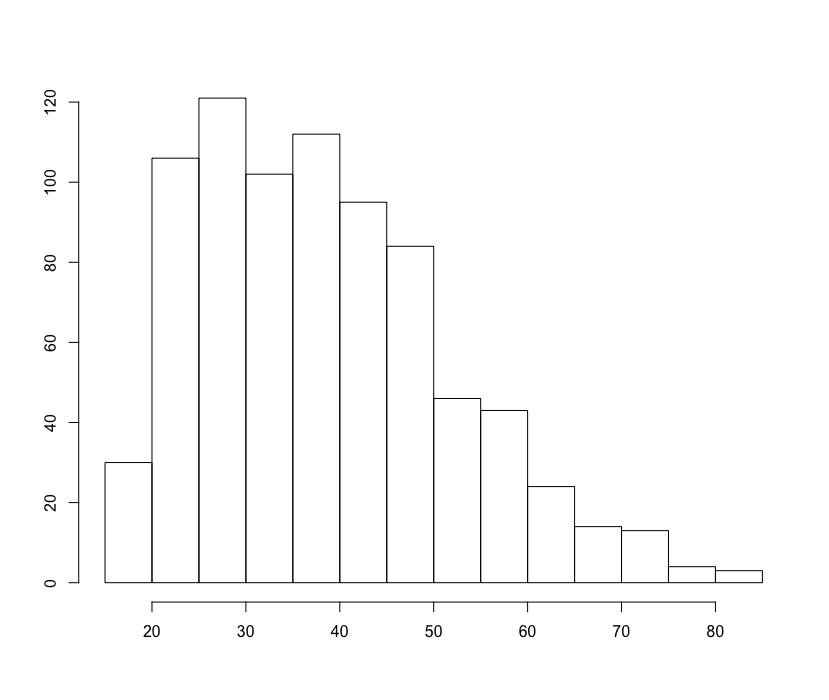
\includegraphics[scale=0.4]{ilu/cd.png}\end{center}\end{figure}
Nous pouvons à présent nous poser la question de la \textit{Normalité} de la distribution. \newline
\\
Certes, le représentation nous montre une allure de courbe en cloche mais néanmoins assymétrique. Vraisemblablement, l'âge ne suit pas une loi Normale.\newline
Bien que nous ayons conclu que cette distribution ne suivait pas une loi Normale, nous aurions pu, si nous avions 20 sujets par groupe, alors qu'\textit{officiellement}, nous ne pouvons utiliser le test de Student, l'appliquer quand même  et celui ci fonctionnerait très bien.\newline
\\
L'analyse graphique d'une distribution n'est pas un critère très rigoureux. On peut donc se poser la question de savoir si il existe une règle qui permet de dire si une distribution suit une loi Normale et si l'on peut utiliser un test t de Student. La réponse est \textbf{non}. Certains statisticiens testeront la normalité de la variable mais cette pratique ne répond pas à la question.\newline
En effet, un test statistique n'est utilisable que si l'on souhaité démontrer que la variable \underline{ne suit pas une loi normale}, c'est là le principal intérêt des tests statistiques. De manière générale, un test statistique ne permettra \textbf{jamais} d'affirmer avec certitude qu'une variable suit une loi Normale. De plus, on sait que l'immense majorité des variables ne suivent pas réellement une loi Normale, cela n'est toujours qu'approximatif.\newline
La vraie question avec le test t de Student est donc \textit{Dans quelle mesure la loi est elle suffisamment normale pour réaliser un test t de Student} mais les statistiques ne répondront jamais à cette question.\newline
\\
Pour essayer d'apporter \textit{une réponse plus rigoureuse à la question de la normalité d'une variable}, les statisticiens proposent de réaliser un \textbf{diagramme de normalité}.\newline
Avec \textbf{R}, pour obtenir un tel diagramme, il faut utiliser les fonctions \textit{qqnorm} et \textit{qqline}.

\begin{lstlisting}[language=html]
qqnorm(smp.c$age)
qqline(smp.c$age)
\end{lstlisting}
\begin{figure}[H]\begin{center}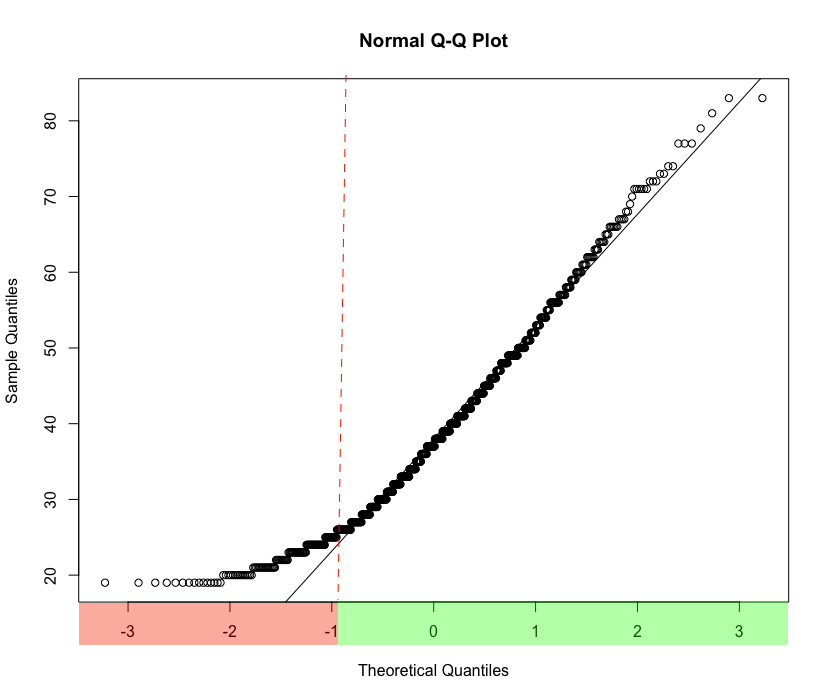
\includegraphics[scale=0.5]{ilu/ce.png}\end{center}\end{figure}
On obtient alors une série de points qui sont normalement tous alignés. On voit ici que c'est le cas pour le milieu de la distribution et sa partie droite. Par contre, pour la partie gauche de la distribution, on peut observer que les points s'écartent de la ligne. \textbf{On a donc localement, un écart à la normalité}.\newline
Les statisticiens dignes de ce nom pensent que cette approche est préférable.\newline
\\
\textbf{Note : } Les deux approches (visualisation de l'histogramme ou du diagramme de normalité) sont valables et leur utilisation varie d'un statisticien à un autre.\newline
\\
\textbf{La normalité n'est pas le seul facteur à prendre en compte.}\newline
\\
En effet, le test t de Student impose également, comme condition de validité, que les variances soient identiques dans les groupes que nous devons comparer.\newline
Il faut donc calculer la variance (ou l'écart type au carré) selon que les individus présentent un niveau élevé (1) ou "normal/faible" (0) d'évitement du danger. \newline
Pour ce faire, nous allons utiliser la fonction \textit{by(variable à étudier, variable qui détermine les sous groupes, fonction que l'on souhaite calculer, le mode de gestion des données manquantes)}.\newline
\\
Vérifions d'abord la relation entre l'écart type et la variance : $\sigma^{2}_{x}=V_{x}$ : 
\begin{lstlisting}[language=html]
> ##Afichage des effectifs par modalité
> table(smp.c$age)

19 20 21 22 23 24 25 26 27 28 29 30 31 32 33 34 35 36 37 38 39 40 41 42 43 
15 15 18 13 23 30 22 30 25 21 20 25 18 22 26 20 16 18 25 24 23 22 23 19 17 
44 45 46 47 48 49 50 51 52 53 54 55 56 57 58 59 60 61 62 63 64 65 66 67 68 
19 17 16 12 17 23 16 11 10  8 11  6 14  9  7  6  7  5  7  4  5  3  6  4  2 
69 70 71 72 73 74 77 79 81 83 1  1  6  3  2  2  3  1  1  2 
> ##Calcul de la variance
> v<-var(table(smp.c$age))
> v
[1] 73.63023
> ##Calcul de l'écart type
> s<-sd(table(smp.c$age))
> s
[1] 8.580806
> ##Vérification s^2=v (arondi à deux décimales)
> (round(s^2,2))==(round(v,2))
[1] TRUE
\end{lstlisting}
Puisque la relation est vérifié, nous allons prendre, au choix, l'écart tupe pour réaliser le calcul permettant d'étudier la condition de validité d'un test t de Student : 
\begin{lstlisting}[language=html]
> by(smp.c$age,smp.c$ed.bin,sd,na.rm=TRUE)
smp.c$ed.bin: 0
[1] 13.38593
-------------------------------------------------------- 
smp.c$ed.bin: 1
[1] 13.29636
\end{lstlisting}
Réalisons le même calcul pour la variance : 
\begin{lstlisting}[language=html]
> by(smp.c$age,smp.c$ed.bin,var,na.rm=TRUE)
smp.c$ed.bin: 0
[1] 179.1831
-------------------------------------------------------- 
smp.c$ed.bin: 1
[1] 176.7933
\end{lstlisting}
Nous pouvons voir que les résultats sont approxivement identiques.\newline
\\
\textbf{Convention : } En statistique, on considère que lorsqu'un écart type est supérieur à $1,5$ fois l'autre écart type, les deux écart types sont différents.
\begin{lstlisting}[language=html]
> x = 13.38593
> y = 13.29636
> (x>=(y)*(1.5))
[1] FALSE
\end{lstlisting}
On peut donc conclure sur l'égalité des deux écart-types.\newline
\\
Maintenant que nous avons démontrer les condition de validité pour effectuer un test t de Student, nous allons pouvoir le calculer.\newline
Pour ce faire, nous allons utiliser la fonction \textit{test.t(variable à étudier $\sim$ variable qui détermine les sous groupes, var.equal = TRUE)}.\newline
Nous utilisons le dernier paramètre car sinon, par défaut \textbf{R} utilise l'approximation de Welch, qui permet d'avoir un test t de Student même quand les variances sont inégales ce qui n'est pas recommandé.
\begin{lstlisting}[language=html]
> t.test(smp.c$age~ smp.c$ed.bin, var.equal = TRUE)

	Two Sample t-test

data:  smp.c$age by smp.c$ed.bin
t = 1.7142, df = 690, p-value = 0.08694
alternative hypothesis: true difference in means is not equal to 0
95 percent confidence interval:
 -0.2710524  4.0005138
sample estimates:
mean in group 0 mean in group 1 
       39.46383        37.59910 
\end{lstlisting}
Comme nous pouvons le constater, la valeur du $p$ est égale à $p0.08694$ donc supérieur à $0,05$ soit $5\%$. On peut donc pas conclure sur le fait qu'il existe une différence statistiquement significative d'âge, entre les détenus qui ont un niveau élevé d'évitement du danger et les détenus qui ont un niveau normal ou faible d'évitement du danger.\newline
la fonction \textit{t.test()} donne également les moyennes des âges en fonction des deux groupes. Nous constatons curieusement que dans le groupe "normal ou faible" d'évitement du danger, la moyenne d'âge est de $39$ ans contre $37,5$ ans dans le groupe "élevé". Au début de cette étude, nous avions supposé le contraire à savoir \textit{avec l'âge, le niveau d'évitement du danger est supérieure}, ce qui n'est pas le cas vu les résultats que nous venons d'obtenir.\newline
La différence entre les âges n'est néanmoins pas significative.\newline
\\
Si nous ne pouvons pas utiliser le test t de Student parce qu'à la fois, nous avons un petit effectif et une variable qui ne suis pas la loi Normale, il est possible d'utiliser le test de \textbf{Mann-Whitney ou de Wilcoxon}.\newline
La fonction \textbf{R} correspondante est la fonction \textit{wilcox.test()} et la syntaxe est très similaire à celle du \textit{t.test()}. Les résultats s'interprètent de la même façon.
\begin{lstlisting}[language=html]
> wilcox.test(smp.c$age~smp.c$ed.bin)

	Wilcoxon rank sum test with continuity correction

data:  smp.c$age by smp.c$ed.bin
W = 56770, p-value = 0.06091
alternative hypothesis: true location shift is not equal to 0
\end{lstlisting}
Nous pouvons remarquer que la différence n'est toujours pas significative car nous obtenons un $p$ égal à environ $6\%$.\newline
\\
En fin de compte, nous pouvons nous demander si le test de Wilcoxon n'est pas une alternative généraliste au test t de Student.\newline
Certains statisticiens pensent que le test de Wilcoxon est un test légèrement moins puissant que le test t et donc qu'il est plus pertinent d'utiliser le test t de Student. Cependant, la différence de puissance entre les deux test n'est pas significative. Nous pourrions donc y gagner à utiliser un test qui fonctionne sans pré conditions.\newline
Cependant, le test de Wilcoxon ne compare pas des moyennes mais des \textbf{rangs d'individus}. On classe les individus et on regarde en moyenne si le rang dans le groupe $A$ est supérieur au rang dans le groupe $B$. Dans le chapitre précédent, nous avons vu qu'interpréter une moyenne n'était pas une chose aisée alors que comparer des rangs d'individus devient une méthode assez abstraite et nous ne sommes pas sûr que tout le monde puisse l'interpréter de manière appropriée.\newline
Enfin, si l'on doit avoir recours à un test de Wilcoxon, cela signifie que l'on est sur que la variable ne suit pas une loi Normale et donc de fait, nous ne pourrons pas utiliser d'analyse de variance, de régression linéaire multiple, \dots car ces méthodes requièrent une normalité de variable que l'on utilise.\newline
Le test de Wilcoxon ne permet donc pas de faire des analyses multivariées ce qui en soit est assez limitatif.
\newpage 

\section{Les tests statistiques en pratique : test de la nullité d'un coefficient de corrélation, divers}
Le \textbf{Test de nullité d'un coefficient de corrélation} ne possède pas de nom défini comme le test du $\chi^{2}$ ou le test de Student.\newline 
Les conditions de validité de ce test sont assez simple. Si nous souhaitons tester la nullité de la corrélation de la variable $x$ avec la variable $y$, il faut que la \textbf{distribution de $x$ ou celle de $y$ suive une loi Normale}. Il n'est donc pas nécessaire que les deux variables suivent une loi Normale mais seulement l'une des deux.\newline
\\
Dans le cadre de l'étude sur la santé mentale en prison, nous allons étudier la corrélation qu'il est susceptible d'avoir entre un âge élevé et un niveau de recherche de sensation faible. En effet,  nous allons partir de l'hypothèse qu'\textit{avec l'âge, les individus recherchent moins de sensations fortes}.\newline
\\
Nous allons donc tester à $0$ cette corrélation et la fonction \textbf{R} correspondante est \textit{cor.test()}. la syntaxe est très simple, on met la première variable puis la seconde après une virgule.

\begin{lstlisting}[language=html]
> setwd("~/Desktop/DIVERS_TEMPLATES/R/TP")
> smp.c <-read.csv2("DONNEES/smp1.csv")
> table(smp.c$age,useNA = "always")

  19   20   21   22   23   24   25   26   27   28   29   30   31   32   33 
  15   15   18   13   23   30   22   30   25   21   20   25   18   22   26 
  34   35   36   37   38   39   40   41   42   43   44   45   46   47   48 
  20   16   18   25   24   23   22   23   19   17   19   17   16   12   17 
  49   50   51   52   53   54   55   56   57   58   59   60   61   62   63 
  23   16   11   10    8   11    6   14    9    7    6    7    5    7    4 
  64   65   66   67   68   69   70   71   72   73   74   77   79   81   83 
   5    3    6    4    2    1    1    6    3    2    2    3    1    1    2 
<NA> 
   2 
> table(smp.c$rs,useNA = "always")

   1    2    3 <NA> 
 249  158  289  103 
> cor.test(smp.c$age,smp.c$rs)

	Pearson's product-moment correlation

data:  smp.c$age and smp.c$rs
t = -6.02, df = 694, p-value = 2.825e-09
alternative hypothesis: true correlation is not equal to 0
95 percent confidence interval:
 -0.2922516 -0.1509579
sample estimates:
       cor 
-0.2227744 
\end{lstlisting}
Les résultats sont classiques : on obtient $p= 2,825.10^{-9}$, inférieur à $10^{-8}$ donc la corrélation est très significativement non nulle. La fonction cor.test() donne également le coefficient de corrélation qui est ici égal à $r=-0,2227744$ ce qui confirme notre hypothèse : \textit{Il y a bien une corrélation négative entre âge et recherche de sensations}.\newline
La fonction cor.test donne également l'intervalle de confiance à $95\%$ de ce coefficient de corrélation. ce dernier est $[-0,2922516, -0,1509579]$. Il signifie que la corrélation de $-0,22$ que l'on vient d'observer correspond à la corrélation des 799 individus. Cet intervalle de confiance permet de répondre à la question : \textit{Quelle est la valeur de la corrélation entre age et recherche de sensation, non pas dans cet échantillon mais plutôt pour l'ensemble de la population des détenus ?} La réponse est donc qu'à $95\%$ de chance, la corrélation se situera dans l'intervalle $[-0,2922516, -0,1509579]$.\newline
\\
Nous avons vu dans le chapitre précédent que la distribution de l'âge des détenus était approximativement Normale mais très asymétrique. Nous pouvons dire que dans le cadre d'une première approximation, la normalité est suffisante pour accepter d'utiliser le test classique de nullité d'un coefficient de corrélation de PEARSON; d'autant plus que la variable \textit{recherche de sensation} ne suit pas du tout une loi normale car c'est une variable qualitative d'état prenant comme valeur $1,2$ ou $3$ :
\begin{itemize}
\item 1 - La recherche de sensation est faible 
\item 2 - La recherche de sensation est moyenne 
\item 3 - La recherche de sensation est forte
\end{itemize}
Pour calculer un test de nullité du coefficient de corrélation, il faut absolument que la variable âge suive une loi Normale car sinon, la condition de validité n'est pas remplie.\newline
Dans le cas où la pré condition est violé, il existe un autre test appelé \textbf{Test de nullité de la corrélation de SPEARMAN} et non plus de Pearson.\newline
La corrélation de SPEARMAN s'intéresse aux rangs des sujets et non plus sur les observations en elles mêmes. Dans notre exemple, nous prenons les âges des sujets que l'on classe de manière croissante et on fait de même pour les niveaux de recherche de sensation. On effectue alors le calcul de la corrélation entre les rangs de l'âge et ceux de la recherche de sensation. Cette méthode est considérée comme beaucoup plus robuste.\newline
\\
Pour effectuer le test de corrélation au sens de SPEARMAN, il suffit d'ajouter \textit{method ="spearman"} à la fonction \textit{cor.test()}.
\begin{lstlisting}[language=html]
> cor.test(smp.c$age,smp.c$rs, method = "spearman")

	Spearman's rank correlation rho

data:  smp.c$age and smp.c$rs
S = 68743000, p-value = 2.567e-09
alternative hypothesis: true rho is not equal to 0
sample estimates:
       rho 
-0.2233474 

Warning message:
In cor.test.default(smp.c$age, smp.c$rs, method = "spearman") :
  Impossible de calculer la p-value exacte avec des ex-aequos
\end{lstlisting}
$p$ vaut alors $2,567.10^{-9}$, toujours considéré comme faible, et la corrélation appelée ici $\rho$ (rho) est très proche de celle que l'on avait obtenue avec le test de nullité du coefficient de corrélation au sens de PEARSON.\newline
\\
A ce stade, il est légitime de ce demander l'utilité du coefficient de corrélation au sens de PEARSON et de sa condition de normalité d'une des deux variables alors que SPEARMAN n'impose aucune pré condition.\newline
\\
Certes, le test de corrélation de SPEARMAN est un peu moins puissant que celui de PEARSON. Nous avons également un autre inconvénient que l'on peut voir sur les résultats de \textbf{R} qui est que les corrélations de SPEARMAN sont "génées" par les ex-aqueo or ici, l'étude engendre de nombreux ex-aqueo car le niveau de recherche de sensation est codé sur trois niveaux. L'impossibilité de la gestion des ex-aqueo est une limite à l'utilisation de la méthode de SPEARMAN.\newline
Enfin, de la même manière qui consiste à réserver le test Wilcoxon à des situations où la normalité de la variable n'est pas définie, si l'on utilise une corrélation de SPEARMAN, ce la signifie que de facto, nous allons considérer que les variables que l'on souhaite correller ne suivent de loi Normale et donc de fait, cela va nous interdire d'utiliser toute technique statistique qui nécessite la normalité de ses variables comme par exemple, une regression linéaire multiple.\newline
Avant de nous interdire l'utilisation de toutes ces méthode, nous devons "peser" les pours et les contres et se demander si l'une des variables (et dans notre cas l'âge) ne suit pas suffisamment une loi Normale, ce qui nous permettrait d'utiliser le coefficient de corrélation de PEARSON et non celui de SPEARMAN.\newline
\\
Nous allons à présent nous intéresser à des tests statistique qui sont moins fréquents mais qui sont cependant utiles et que nous nous devons de connaître dans le cas où nous nous retrouverions dans des cas \textit{délicats}.\newline 
\\
La première de ces situations concerne la \textbf{comparaison d'une moyenne à une moyenne de référence}.\newline
De manière générale, nous ne connaissons pas la valeur de référence d'un paramètre dans une population mais dans certain cas, c'est la cas. Prenons l'exemple du QI : Pour un âge donné, on sait que la moyenne du QI est égale à $100$. Dans le cadre d'un groupe de patients hyperactif, on peut être amené à nous demander si la moyenne de leurs QI est conforme à celle de la population de référence; Il suffit juste de comparer la moyenne du QI de nos patient à 100.\newline
La syntaxe de \textbf{R} dans ces cas est \textit{t.test()} dans laquelle nous indiquons la variable du QI.\newline
Dans la cas suivant, Nous n'avons que les âges de la population. On pose $\mu = 24 $ (mu). Dans le cas où nous étudierions le QI de nos patient avec une moyenne à $100$, on aurait $\mu = 100$.
\begin{lstlisting}[language=html]
> t.test(smp.c$age, mu = 24)

	One Sample t-test

data:  smp.c$age
t = 31.672, df = 796, p-value < 2.2e-16
alternative hypothesis: true mean is not equal to 24
95 percent confidence interval:
 37.97618 39.82307
sample estimates:
mean of x 
 38.89962 
\end{lstlisting}
\textcolor{white}{.}\newline
Le second cas concerne les tests dit \textbf{appariés}. La plupart des cas où l'on a recours à des tests appariés sont des situations dans lesquelles nous avons des mesures dites \textit{avant/après} c'est à dire que l'on étudie l'évolution d'une population au cours du temps.\newline
On peut discerner deux cas : 
\begin{itemize}
\item \textbf{Cas des variables qualitatives}\newline 
Si nous prenons par exemple l'étude du niveau de sport des hommes avant et après leurs mariages, nous allons suivre un groupe de $N$ hommes puis nous allons comparer le pourcentage de sportifs avant le mariage au pourcentage de sportifs après le mariage.\newline
Nous pourrions éventuellement envisager un test du $\chi^{2}$ (comparaison de pourcentages) mais ce dernier\textbf{ne va pas tenir compte de l'évolution} des hommes dans le temps (avant et après le mariage) et que ce sont les mêmes sujets que l'on étudie en deux temps distincts. En somme, le résultat de ce test ne sera pas totalement faux mais il ne prendra	pas en compte le fait que chaque sujet est son propre contrôle.\newline
Pour répondre à ce type de problème, nous pouvons utiliser le \textbf{test de MACNEMAR}. La fonction \textbf{R} correspondante est \textit{mcnemar.test()} et l'on y indique en paramètre les valeurs dites d'avant (b.debut) et d'après (b.fin) et il retourne une valeur de $p$:
 \begin{lstlisting}[language=html]
> b.debut = c(1,3)
> b.fin = c(3,2)
> mcnemar.test(b.debut,b.fin)

	McNemar's Chi-squared test

data:  b.debut and b.fin
McNemar's chi-squared = 0, df = 1, p-value = 1

> data <- matrix(c(1, 4, 2, 3), ncol=2, byrow=T)
> data
     [,1] [,2]
[1,]    1    4
[2,]    2    3
> mcnemar.test(data)

	McNemar's Chi-squared test with continuity correction

data:  data
McNemar's chi-squared = 0.16667, df = 1, p-value = 0.6831

> data <- matrix(c(25, 5, 15, 15), ncol=2, byrow=T)
> data2 <- matrix(c(16, 11, 3, 21, 8, 1), ncol=2, byrow=T)
> mcnemar.test(data)

	McNemar's Chi-squared test with continuity correction

data:  data
McNemar's chi-squared = 4.05, df = 1, p-value = 0.04417

> chisq.test(data)

	Pearson's Chi-squared test with Yates' continuity correction

data:  data
X-squared = 6.075, df = 1, p-value = 0.01371

> mcnemar.test(data2)
Error in mcnemar.test(data2) : 
  'x' doit être carrée avec au moins deux lignes et deux colonnes
> chisq.test(data2)

	Pearson's Chi-squared test

data:  data2
X-squared = 19.465, df = 2, p-value = 5.932e-05

Warning message:
In chisq.test(data2) : l'approximation du Chi-2 est peut-être incorrecte
\end{lstlisting}


\item \textbf{Cas des variables quantitatives}\newline
Cas beaucoup plus fréquent des test appariés, on l'utilise pour par exemple, suivre l'évolution du QI d'un enfant avant et après une technique de rééducation. On peut également comparer les revenus d'individus à 30 et 40 ans. Si nous utilisons un test de STUDENT, nous n'allons pas tenir compte du fait que la population est la même aux deux moments (avant/après) de l'étude et nous serons en situation de sous puissance. Il faut donc utiliser le \textbf{Test de Student aux populations appariées}.\newline
La fonction \textbf{R} correspondante est \textit{t.test()} dans laquelle on définit les valeurs avant et après suivi de l'instruction \textit{paired = TRUE}.

\begin{lstlisting}[language=html]
> x.debut =c(22,24,45,34,67,34)
> x.fin =c(72,94,45,14,63,33)
> t.test(x.debut,x.fin, paired = TRUE)

	Paired t-test

data:  x.debut and x.fin
t = -1.0915, df = 5, p-value = 0.3248
alternative hypothesis: true difference in means is not equal to 0
95 percent confidence interval:
 -53.12252  21.45586
sample estimates:
mean of the differences 
              -15.83333 
\end{lstlisting}
\end{itemize}
\newpage
\section{Régression linéaire "simple"}
Nous allons à présent commencer une série de chapitres sur la régression linéaire et l'analyse de variances en débutant par le \textbf{cas particulier de la régression linéaire simple}.\newline
\\
A ce stade, nous allons avoir besoin d'une version du fichier \textit{santé mentale en prison} plus complète. Ce nouveau fichier s'appelle \textit{smp.2.csv} et contient toujours $26$ variables sur $799$ sujets.\newline
\begin{lstlisting}[language=html]
> setwd("~/Desktop/DIVERS_TEMPLATES/R/TP")
> smp <- read.csv2("DONNEES/smp2.csv")
> str(smp)
'data.frame':	799 obs. of  26 variables:
 $ age         : int  31 49 50 47 23 34 24 52 42 45 ...
 $ prof        : Factor w/ 8 levels "agriculteur",..: 3 NA 7 6 8 6 3 2 6 6 ...
 $ duree       : int  4 NA 5 NA 4 NA NA 5 4 NA ...
 $ discip      : int  0 0 0 0 1 0 0 0 1 0 ...
 $ n.enfant    : int  2 7 2 0 1 3 5 2 1 2 ...
 $ n.fratrie   : int  4 3 2 6 6 2 3 9 12 5 ...
 $ ecole       : int  1 2 2 1 1 2 1 2 1 2 ...
 $ separation  : int  0 1 0 1 1 0 1 0 1 0 ...
 $ juge.enfant : int  0 0 0 0 NA 0 1 0 1 0 ...
 $ place       : int  0 0 0 1 1 0 1 0 0 0 ...
 $ abus        : int  0 0 0 0 0 0 0 0 1 1 ...
 $ grav.cons   : int  1 2 2 1 2 1 5 1 5 5 ...
 $ dep.cons    : int  0 0 0 0 1 0 1 0 1 0 ...
 $ ago.cons    : int  1 0 0 0 0 0 0 0 0 0 ...
 $ ptsd.cons   : int  0 0 0 0 0 0 0 0 0 0 ...
 $ alc.cons    : int  0 0 0 0 0 0 0 0 1 1 ...
 $ subst.cons  : int  0 0 0 0 0 0 1 0 1 0 ...
 $ scz.cons    : int  0 0 0 0 0 0 0 0 0 0 ...
 $ char        : int  1 1 1 1 1 1 1 1 4 1 ...
 $ rs          : int  2 2 2 2 2 1 3 2 3 2 ...
 $ ed          : int  1 2 3 2 2 2 3 2 3 2 ...
 $ dr          : int  1 1 2 2 2 1 2 2 1 2 ...
 $ suicide.s   : int  0 0 0 1 0 0 3 0 4 0 ...
 $ suicide.hr  : int  0 0 0 0 0 0 1 0 1 0 ...
 $ suicide.past: int  0 0 0 0 1 0 1 0 1 0 ...
 $ dur.interv  : int  NA 70 NA 105 NA NA 105 84 78 60 ...
\end{lstlisting}
Nous retrouvons les variables suivantes : 
\begin{itemize}
\item \textit{age} : l'âge des détenus 
\item \textit{prof} : la profession des détenus  
\item \textit{duree} : la durée de la détention d'un individu  
\item \textit{discip} : Est ce que le détenu est sous mesure disciplinaire  
\item \textit{n.enfant} : Le nombre d'enfant
\item \textit{n.fraterie} : La taille de la fraterie du détenu 
\item \textit{ecole} : la variable relative à la scolarisation du détenu (comprise entre $1$ et $5$) 
\item \textit{separation} : Est ce que le détenu a été séparé de sa famille lorsqu'il était enfant (\textit{oui} ou \textit{non})
\item \textit{juge.enfant} : Est ce que le détenu a bénéficier de l'aide d'un juge pour enfant lorsqu'il était enfant  
\item \textit{place} : Est ce que le détenu a été placé lorsqu'il était enfant 
\item \textit{abus} : Est ce que le détenu a été victime d'abus 
\end{itemize}
Nous retrouvons également les variables de diagnostic :
\begin{itemize}
\item \textit{grav.cons} : La gravité consensuelle de la maladie du détenu
\item \textit{dep.cons} : L'existence d'une dépression chez le détenu  
\item \textit{ago.cons} : L'existence d'un trouble agoraphobique chez le détenu  
\item \textit{ptsd.cons} : L'existence d'un syndrôme de stress post - traumatique chez le détenu 
\item \textit{alc.cons} : L'existence d'un abus d'alcool chez le détenu 
\item \textit{subst.cons} : L'existence d'un abus de susbtance chez le détenu 
\item \textit{scs.cons} : L'existence d'un trouble schizophrénique chez le détenu  
\end{itemize}
Et enfin, nous retrouvons les variables de personnalité suivantes : 
\begin{itemize}
\item \textit{char} : Variable qui correspnd à un score semi-quantitatif qui évalue l'importance et l'intensité d'un trouble de la personnalité sous-jacent 
\item \textit{rs} : Le niveau de recherche de sensations chez un détenu
\item \textit{ed} : Le niveau d'évitemment du risque chez un détenu
\item \textit{dr} : Le niveau de dépendance à la récompense chez un détenu
\item \textit{suicide.s} : Le score de risque suicidaire d'un détenu
\item \textit{suicide.hr} : L'existence d'un haut risque suicidaire - Binarisation de la variable \textit{suicide.s} 
\item \textit{suicide.past} : L'existence d'antécédents de tentative de suicide chez un patient 
\item \textit{dur.interv} : La durée de l'entretien que les enquêteurs ont passée avec le détenu 
\end{itemize}
Dans notre cursus secondaire, nous avons étudier des droites de regressions, très prisées par la communauté des physiciens.\newline
Dans le cas où nous avons un nuage de point dans le plan, \textbf{la droite de regression est la droite qui passe, aux mieux, par l'ensemble des points}.
\begin{figure}[H]\begin{center}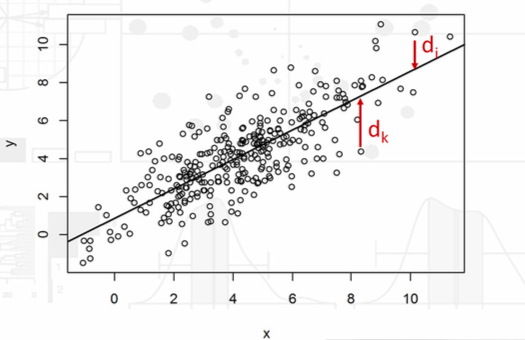
\includegraphics[scale=0.7]{ilu/cl.png}\end{center}\end{figure}
Formellement, la définition mathématique de la droite de régression correspond, pour tout point $i$, au projeté de ce point, parallèlement à l'axe des ordonnées, sur la droite de régression (comme sur le graphique ci dessus) et on appellera $d_{i}$, la distance entre le point $i$ et sa projection sur la droite.\newline
La définition de la droite de régression est la droite qui minimise la somme des distances $d_{i}$ entre le point et sa projection sur sa droite, c'est à dire : 
$$\textrm{argmin} (d_{1}^{2}+ \dots + d_{n}^{2}) =  \textrm{argmin} (\sum_{k=1}^{n}d_{k}^{2})$$
Il est donc très facile de représenter graphiquement et de calculer une droite de régression linéaire avec \textbf{R}.\newline
Nous allons représenter la droite de régression linéaire avec pour valeur de $x$, l'âge des détenus et pour $y$, la durée des entretiens que les enquêteurs ont passé avec les détenus.\newline
Dans un premier temps, on représente le diagramme $x/y$, c'est à dire les âges en fonction de la durée des entretiens grâce à la fonction \textit{plot()} :
\begin{lstlisting}[language=html]
plot(smp$age,smp$dur.interv) 
\end{lstlisting}
\begin{figure}[H]\begin{center}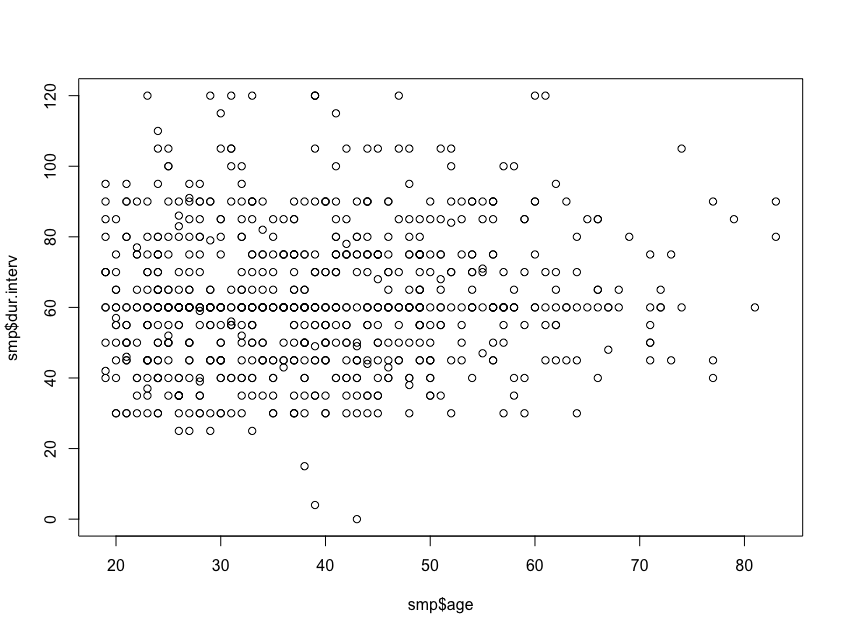
\includegraphics[scale=0.35]{ilu/cm.png}\end{center}\end{figure}
Certes, le graphique est intéressant; Cependant, nous pouvons voir que les valeurs pour les $799$ ne sont pas représentées (comme les variables sont discrètes, les points sont superposés les uns sur les autres dans le cas d'une même observation). Pour remédier à ce problème, nous pouvons utiliser la fonction \textit{jitter()}
\begin{lstlisting}[language=html]
plot(jitter(smp$age),jitter(smp$dur.interv))
\end{lstlisting}
\begin{figure}[H]\begin{center}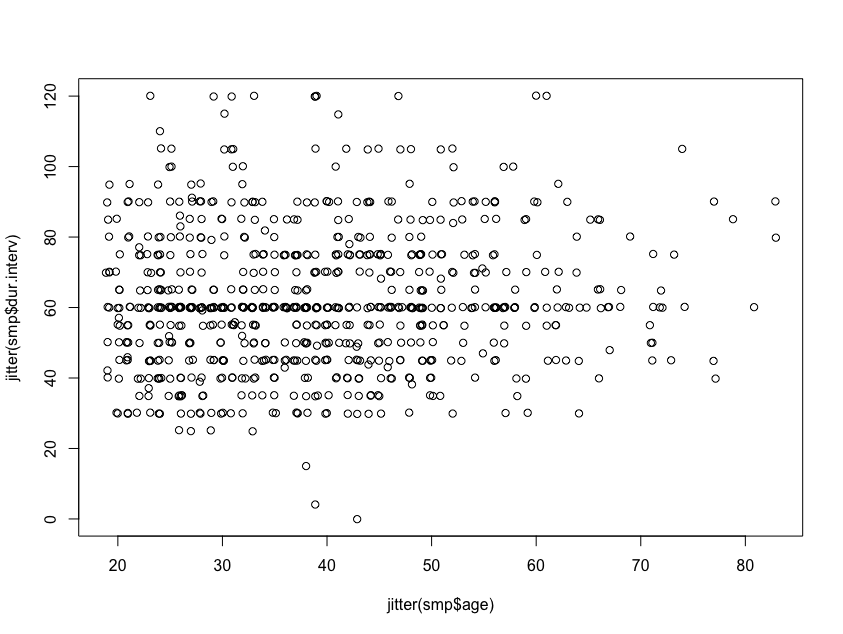
\includegraphics[scale=0.35]{ilu/cn.png}\end{center}\end{figure}
Le graphique obtenu de la sorte est déjà plus informatif.\newline
Cependant, nous pouvons avoir l'impression que le niveau de \textit{bruit} que le logiciel met par défaut sur les valeurs des âges et sur la durée des entretiens est trop petit et que l'on observe encore des points superposés. Il faut savoir qu'il est possible de modifier \underline{à volonté} l'importance du bruit dans la fonction \textit{jitter()} en ajoutant l'attribut \textit{factor = }.\newline
Pour une valeur de \textit{factor} égale à 4, on obtient : 
\begin{lstlisting}[language=html]
plot(jitter(smp$age),jitter(smp$dur.interv,factor=4))
\end{lstlisting}
\begin{figure}[H]\begin{center}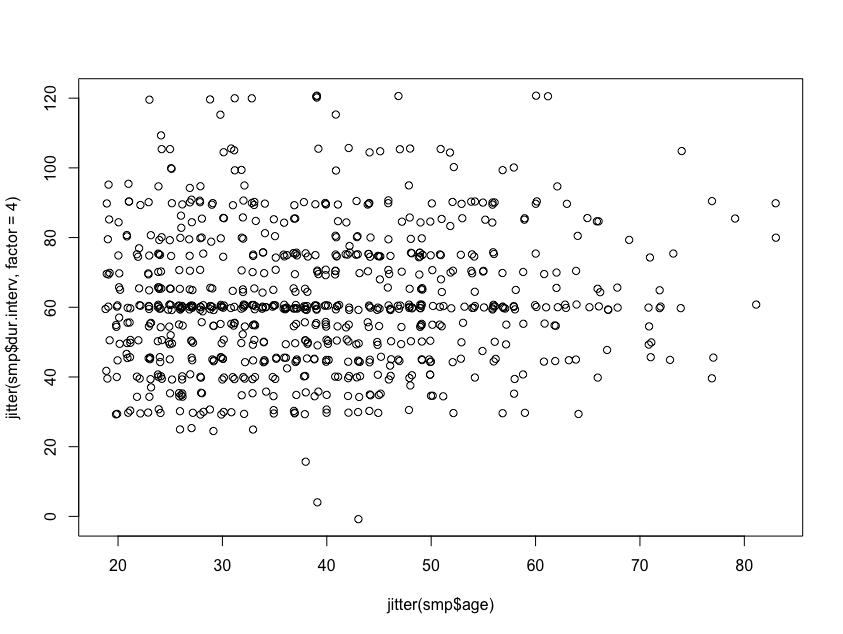
\includegraphics[scale=0.35]{ilu/co.png}\end{center}\end{figure}
Pour une valeur de \textit{factor} égale à 8, on obtient : 
\begin{figure}[H]\begin{center}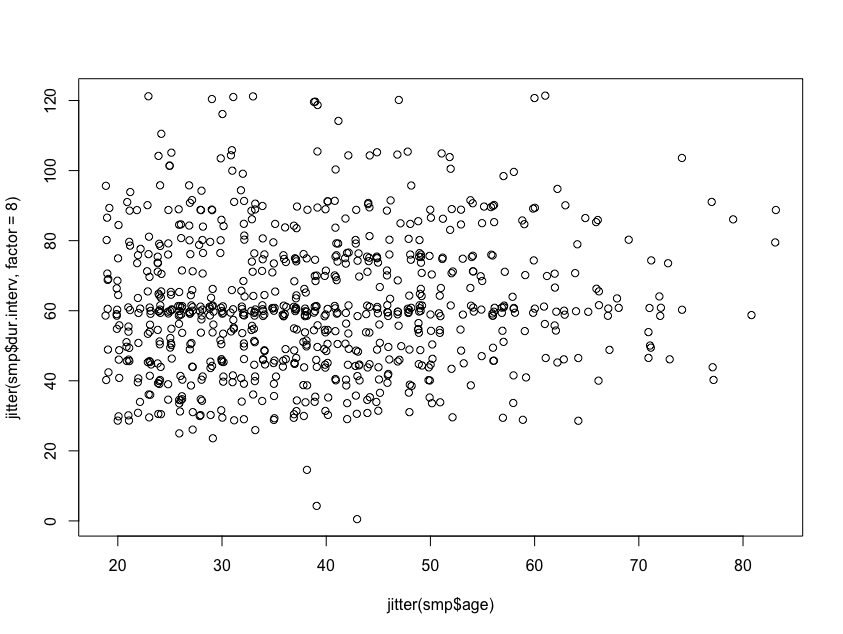
\includegraphics[scale=0.35]{ilu/cp.png}\end{center}\end{figure}
Pour une valeur de \textit{factor} égale à 64, on obtient : 
\begin{figure}[H]\begin{center}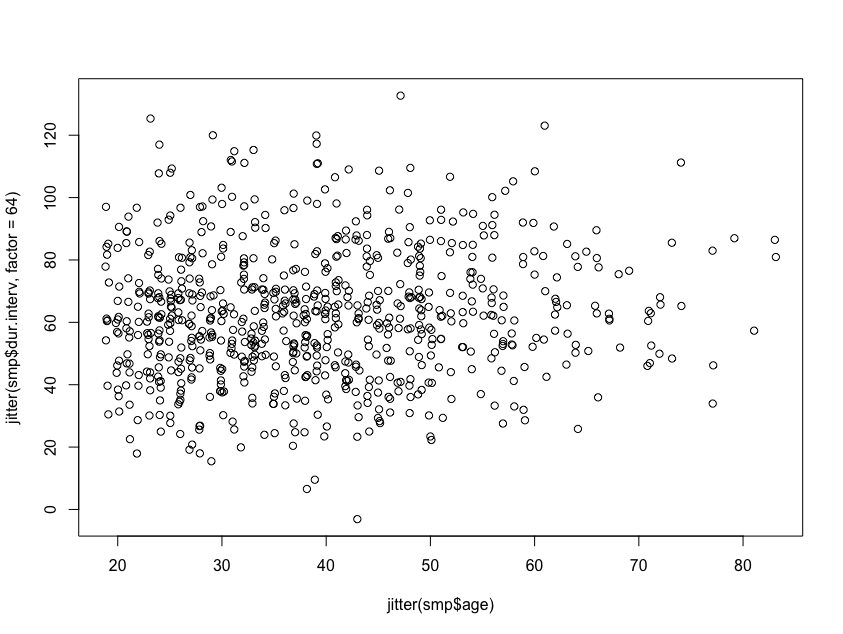
\includegraphics[scale=0.35]{ilu/cq.png}\end{center}\end{figure}
Pour une valeur de \textit{factor} égale à 64, on obtient : 
\begin{figure}[H]\begin{center}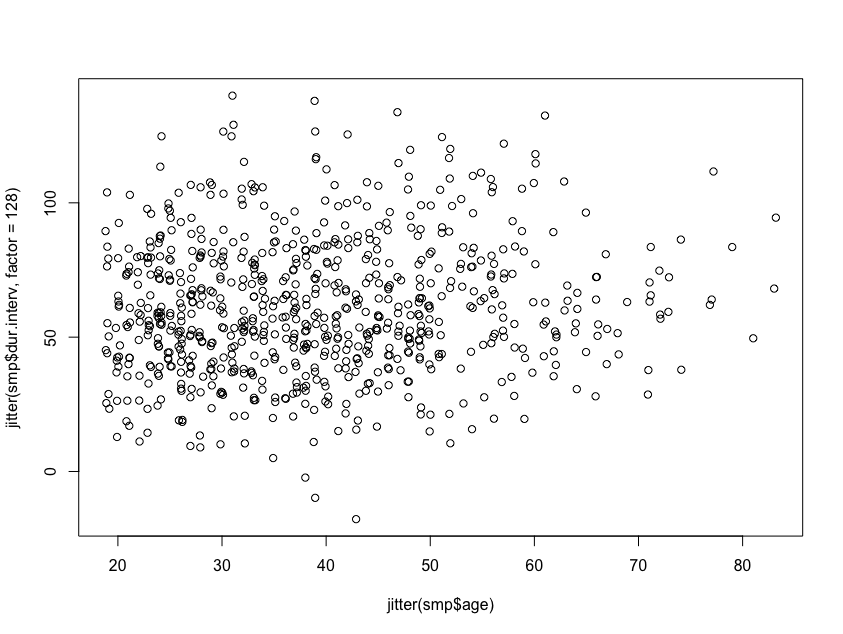
\includegraphics[scale=0.35]{ilu/cr.png}\end{center}\end{figure}
Reprenons le graphique obtenu pour une valeur de \textit{factor} égale à 4.\newline
\\
Pour tracer une droite de régression linéaire sur un nuage de points, nous devons utiliser la double fonction \textit{abline(lm())} : 
\begin{itemize}
\item La fonction \textit{lm()} permet de calculer les coordonnées de la droite de régression linéaire, les coefficients $a$ et $b$ pour une droite d'équation de la forme : 
$$y= b\times x + a$$
\item la fonction \textit{abline()} permet de tracer la droite de régression linéaire 
\item l'attribut \textit{lwd = 2} permet de préciser l'épaisseur de la droite de régression sur le graphique.
\end{itemize}

\begin{lstlisting}[language=html]
abline(lm(smp$dur.interv~smp$age),lwd=2)
\end{lstlisting}	
\begin{figure}[H]\begin{center}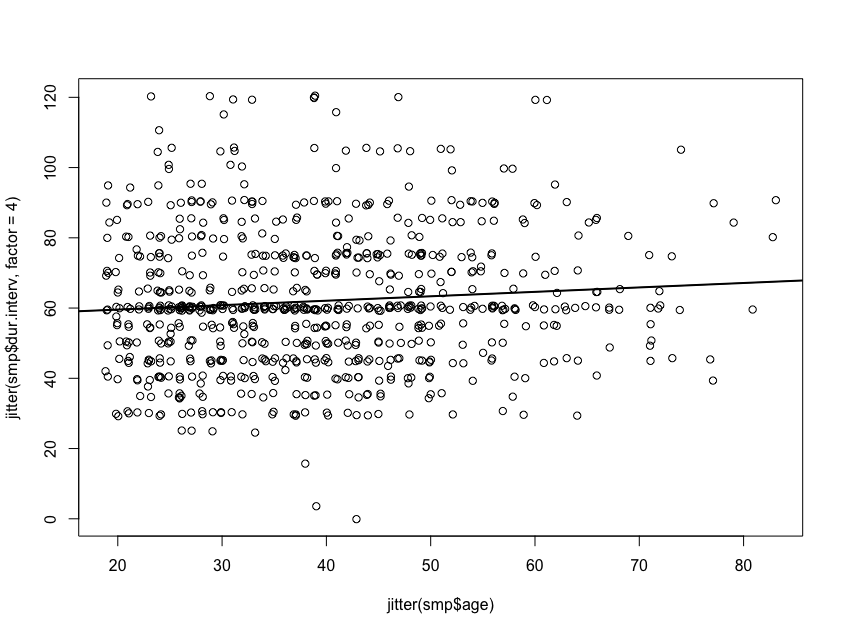
\includegraphics[scale=0.35]{ilu/cs.png}\end{center}\end{figure} 
On peut constater que la droite de régression est quasiment parallèle à l'axe des abscisses mais croissante. \newline
La question que nous pouvons nous poser est alors : \textit{La droite de régression linéaire est elle réellement croissante ou parallèle à l'axe des abscisses ?}\newline
\\
Pour répondre à cette question, ce qui revient à savoir si le coefficient $b$ est statistiquement différent de $0$, nous allons devoir étudier non pas la droite de régression linéaire mais plutôt \textbf{le modèle de régression linéaire}.\newline
\\
La différence entre les deux notions vient du fait que dans le modèle, on prend en compte une \textbf{fonction de bruit} que l'on ajoute à la forme générale $y =b\cdot x + a$.\newline On considère que cette fonction de bruit va suivre une \textbf{Loi Normale}. Grâce à cela, il va nous être possible de savoir si, statistiquement, $b = 0$ à l'aide d'un test de $p-value$ et comparer ce dernier au risque $\alpha$ de $5\%$.\newline
\\
La fonction du logiciel \textbf{R} qui permet d'estimer un modèle de régression linéaire est également la fonction \textit{lm()} que l'on a utilisé précédemment (lm pour linear model).\newline
Sa synthaxe a été présentée précédemment : 
\begin{itemize}
\item la variable $y$ représente la durée de l'entretien
\item le $\sim$ permet de lier les deux variables que l'on souhaite étudier (a$\sim$b, b en fonction de a)
\item la variable $x$ représente l'âge
\item \textit{data=smp} représente l'endroit où sont stockées les données
\end{itemize} 
\begin{lstlisting}[language=html]
> mod <- lm(dur.interv~age,data=smp)
> summary(mod)

Call:
lm(formula = dur.interv ~ age, data = smp)

Residuals:
    Min      1Q  Median      3Q     Max 
-62.470 -14.402  -1.712  12.341  60.055 

Coefficients:
            Estimate Std. Error t value Pr(>|t|)    
(Intercept) 57.04091    2.22028  25.691   <2e-16 ***
age          0.12625    0.05375   2.349   0.0191 *  
---
Signif. codes:  0 ?***' 0.001 ?**' 0.01 ?*' 0.05 ?.' 0.1 ? ' 1

Residual standard error: 19.57 on 745 degrees of freedom
  (52 observations deleted due to missingness)
Multiple R-squared:  0.00735,	Adjusted R-squared:  0.006018 
F-statistic: 5.516 on 1 and 745 DF,  p-value: 0.0191
\end{lstlisting}
\textbf{Note : } Dans le cas présent, on préfèrera stocker l'ensemble des résultats issus de la fonction \textit{lm()} dans une objet. L'opérateur d'affectation est le même qu'en pseudo code algorithmique : \textit{<-}. \newline
Ce choix permet d'estimer le modèle de régression de stocker tous les résultats issus de ce modèle dans un objet et d'appeler après des sous objets de cet objet et ceci, les uns après les autres.\newline
Pour obtenir une vision globale des résultats de la fonction \textit{lm()}, on peut utiliser la fonction \textit{summary()} sur l'objet que l'on souhaite étudier et l'on obtient : 
\begin{itemize}
\item Le coefficient directeur de la droite de régression linéaire $b$ égal à $0,12$
\item L'ordonnée à l'origine de la droite de régression linéaire $a$ égal à $57$ (Nommé \textit{Intercept})
\end{itemize}
On obtient donc la droite de régression linéaire d'équation suivante : 
$$y = 0,12\times x + 57$$
On peut interpréter ces résultats comme le fait qu'à chaque fois qu'un détenu prend une année supplémentaire, les entretiens qu'il aura avec les enquêteurs augmenteront en moyenne de $0,12$ minutes.\newline
On peut également visualiser la valeur de $p$ qui on le rappelle, permet de savoir si \textit{b est significativement différent de 0}? Le résultat obtenu est $p=1,9\%$ soit $p<5\%$. On peut donc en déduire qu'au risque de $5\%$, la pente de la droite de régression linéaire entre la durée de l'entretien et l'âge est significativement différente de $0$.
\newpage
\section{Régression Linéaire : au-delà de la corrélation et du test t}
Dans ce second chapitre sur la régression linéaire, nous allons voir que cette méthode statistique comporte comme cas particulier le test de nullité d'un coefficient de corrélation ainsi que le test t de STUDENT.\newline
\\
Dans le chapitre précédent, nous avons estimé un modèle de régression linéaire simple qui associait la durée des entretiens avec l'âge des détenus sous la forme d'une équation simple de type 
$$y=b\cdot x + a + \textrm{bruit}$$
Nous avons calculé a puis b, b étant égal à $0,12$, c'est à dire proche de $0$. De plus, nous avons testé si $b$ était statistiquement différent de $0$ et la valeur de $p$ pour ce test était de $1,9\%$, $p<5\%$; Nous en avons donc conclu qu'avec un risque de $5\%$, b est statistiquement différent de $0$.\newline
\\
Nous pouvons donc à présent nous pencher sur l'interprétation de la différence de $b$ avec $0$ au sens statistique.\newline
L'interprétation naturelle qui découle de l'équation de regression est de dire que lorsque l'âge du détenu augmente, en moyenne, la durée de l'entretien réalisé avec les cliniciens augmente elle aussi (de $0,12$).\newline
Cependant, si nous avions calculé la corrélation entre la durée de l'entretien et l'âge du détenu et que nous obtenions une corrélation positive, nos conclusions auraient été identiques.\newline
Nous avons donc deux tests statistiques qui testent la même hypothèse exactement. Nous pouvons donc espérer que les résultats (valeurs de $p$) soient proches. Nous allons donc le vérifier puis tester la nullité de la corrélation entre la durée des entretiens et l'âge.\newline
\\
Nous rappellons les résultats obtenus précédemment : 
\begin{lstlisting}[language=html]
> mod <- lm(dur.interv~age,data=smp)
> summary(mod)

Call:
lm(formula = dur.interv ~ age, data = smp)

Residuals:
    Min      1Q  Median      3Q     Max 
-62.470 -14.402  -1.712  12.341  60.055 

Coefficients:
            Estimate Std. Error t value Pr(>|t|)
(Intercept) 57.04091    2.22028  25.691   <2e-16
age          0.12625    0.05375   2.349   0.0191
               
(Intercept) ***
age         *  
---
Signif. codes:  
0 ?***' 0.001 ?**' 0.01 ?*' 0.05 ?.' 0.1 ? ' 1

Residual standard error: 19.57 on 745 degrees of freedom
  (52 observations deleted due to missingness)
Multiple R-squared:  0.00735,	Adjusted R-squared:  0.006018 
F-statistic: 5.516 on 1 and 745 DF,  p-value: 0.0191
\end{lstlisting}
Pour calculer la seconde corrélation, nous allons utiliser la fonction \textit{cor.test()} : 

\begin{lstlisting}[language=html]
> cor.test(smp$age,smp$dur.interv)

	Pearson's product-moment correlation

data:  smp$age and smp$dur.interv
t = 2.3487, df = 745, p-value = 0.0191
alternative hypothesis: true correlation is not equal to 0
95 percent confidence interval:
 0.01408787 0.15650345
sample estimates:
       cor 
0.08573358 
\end{lstlisting}
Nous pouvons remarquer que dans les deux tests, la valeur de $p$ est égale à $1,91\%$. La conclusion des test est exactement la même à savoir \underline{$b \neq 0$}.\newline
\\
Dans les résultats obtenus ci dessus, nous avons une valeur de la corrélation entre la durée des entretiens et l'âge vaut $0,085$, la valeur du coefficient directeur de la droite de régression linéaire $b=0,12$. On peut donc en conclure qu'il existe une équation mathématique qui lie ces deux valeurs.\newline
Dans ce cas, la corrélation est : 
$$r = b \times \frac{\sigma_{\textrm{âge}}}{\sigma_{\textrm{durée entretiens}}}$$

Nous pouvons donc nous demander, puisque les valeurs de $p$ obtenues pour un test de nullité de la corrélation et le test $b=0$ sont identiques et qu'il nous est possible de déduire la valeur de $b$, si il est vraiment pertinent de réaliser des régressions linéaires simples.\newline 
\begin{lstlisting}[language=html]
> mod <- lm(dur.interv~age,data=smp)
> summary(mod)

Call:
lm(formula = dur.interv ~ age, data = smp)

Residuals:
    Min      1Q  Median      3Q     Max 
-62.470 -14.402  -1.712  12.341  60.055 

Coefficients:
            Estimate Std. Error t value Pr(>|t|)    
(Intercept) 57.04091    2.22028  25.691   <2e-16 ***
age          0.12625    0.05375   2.349   0.0191 *  
---
Signif. codes:  0 ?***' 0.001 ?**' 0.01 ?*' 0.05 ?.' 0.1 ? ' 1

Residual standard error: 19.57 on 745 degrees of freedom
  (52 observations deleted due to missingness)
Multiple R-squared:  0.00735,	Adjusted R-squared:  0.006018 
F-statistic: 5.516 on 1 and 745 DF,  p-value: 0.0191
\end{lstlisting}

En faveur de la régression linéaire simple : comme nous pouvons le voir dans cette portion de code, nous obtenons directement les valeurs de $b$ et de $a$ pour établir une régression linéaire simple avec $a=57,04$ et $b=0,126$ d'équation : 

$$y = 0,126\cdot b + 57,04 + \textrm{bruit}$$

De plus, le $b$ a une interprétation concrète à savoir : \textit{Par rapport à un groupe de détenus d'âge donné, si l'on analyse les résultats pour un autre groupe de détenus ayant un an de plus, la durée des entretiens augmentent de $0,12$ minutes}. Il serait également possible de dire que \textit{par rapport à un groupe de détenus qui ont un âge donné et un autre groupe qui à 10 ans de plus, l'augmentation de la durée des entretiens est de $10\times b$ soit $1,2$ minutes}.\newline
Cependant, nous allons voir à présent que la régression linéaire simple \textbf{englobe plusieurs méthodes.}\newline
\\
Intéressons nous maintenant à un nouvel exemple qui peut sembler étrange au premier regard mais le résultat final est intéressant.\newline Nous conservons la même variable $y$ à savoir la \textit{durée des entretiens} mais pour la variable $x$, nous prenons à présent la \underline{variable qualitative binaire} \textit{Dépression consensuelle} (absence (0) ou présence (1) de dépression). Nous allons à présent en faire une représentation graphique : 
\begin{lstlisting}[language=html]
> table(smp$dep.cons)

  0   1 
482 317 
> plot(jitter(smp$dep.cons,factor=1),jitter(smp$dur.interv,factor=4))
> abline(lm(smp$dur.interv~smp$dep.cons),lwd=2,col="red")
\end{lstlisting}
\begin{figure}[H]\begin{center}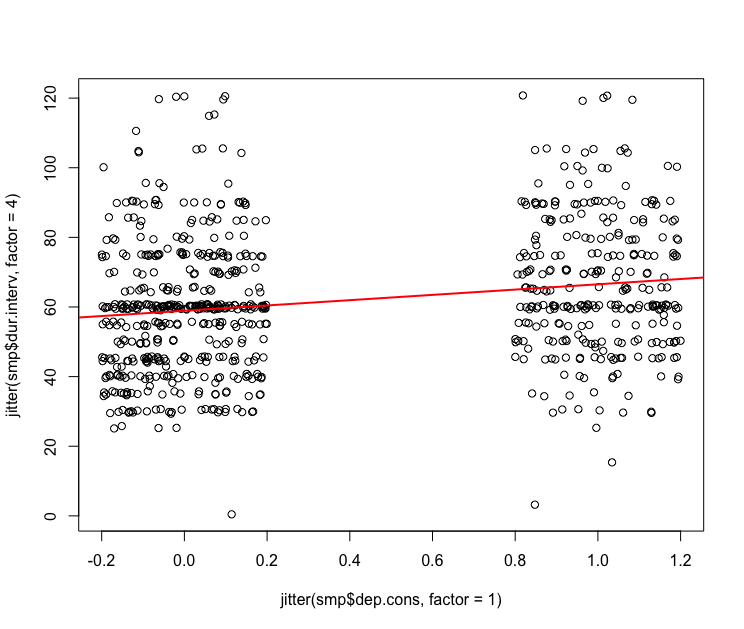
\includegraphics[scale=0.5]{ilu/ct.png}\end{center}\end{figure}
Nous avons donc estimé le modèle de regression suivant : 

$$ y = a + b\times x, b \neq 0$$ 
Où $x$ correspond à la présence de dépression et $y$, la durée des entretiens. Nous reviendrons plus tard sur les conditions de validité pour l'application du modèle de régression linéaire simple.\newline 
\\
Traditionellement, $b$ représente le facteur qui \textit{lorsque la variable de dépression augmente d'un point, alors la variable augmente de $b$ points} comme nous l'avons vu dans l'exemple précédent.\newline
Dans ce cas, lorque la variable depression augmente d'un point, alors nous passons d'absence d'état dépressif à présence de ce dernier.\newline 
Donc la variation correspondante de durée est en fait égale à la variation de durée des entretiens entre les groupes des détenus présentant une symptomatologie dépressive et ceux n'en présentant pas.\newline 
On peut cependant se poser la question concernant la valeur de $b$; Si cette dernière correspond à la différence de durée des entretiens entre les deux types de détenus, si nous testons $b\neq 0$, alors nous devrions théoriquement obtenir les mêmes durées pour chaque détenu, comme si nous utilisions un test t de STUDENT qui comparent la moyenne des durées d'entretien entre les détenus dépressifs et ceux non dépressifs.\newline
\begin{lstlisting}[language=html]
> mod <- lm(dur.interv~dep.cons,data = smp)
> summary(mod)

Call:
lm(formula = dur.interv ~ dep.cons, data = smp)

Residuals:
    Min      1Q  Median      3Q     Max 
-62.538 -13.923   1.077  12.077  61.077 

Coefficients:
            Estimate Std. Error t value Pr(>|t|)    
(Intercept)  58.9234     0.9041  65.171  < 2e-16 ***
dep.cons      7.6143     1.4481   5.258  1.9e-07 ***
---
Signif. codes:  0 ?***' 0.001 ?**' 0.01 ?*' 0.05 ?.' 0.1 ? ' 1

Residual standard error: 19.33 on 747 degrees of freedom
  (50 observations deleted due to missingness)
Multiple R-squared:  0.03569,	Adjusted R-squared:  0.0344 
F-statistic: 27.65 on 1 and 747 DF,  p-value: 1.9e-07

> t.test(smp$dur.interv~smp$dep.cons, var.equal =TRUE)

	Two Sample t-test

data:  smp$dur.interv by smp$dep.cons
t = -5.2583, df = 747, p-value = 1.9e-07
alternative hypothesis: true difference in means is not equal to 0
95 percent confidence interval:
 -10.457001  -4.771515
sample estimates:
mean in group 0 mean in group 1 
       58.92341        66.53767 
\end{lstlisting}
On peut remarquer que nous obtenons les mêmes valeurs de $p$ mais également, que la différence des moyennes entre les deux groupes obtenues avec la fonction \textit{t.test()} retourne une valeur égale à celle de $b$ ($b = 7.6143$ et $|58.9234-66.53767| = 7.61427$).\newline
Nous pouvons donc conclure que réaliser un modèle de régression linéaire simple (durée de l'entretien en fonction de la présence d'une symptomatologie dépressive) retourne des résultats identiques à ceux obtenues par comparaison des moyennes dans le cadre du test t.\newline
Nous avions vu précédemment que la régression linéaire simple était une \textbf{généralisation du test de nullité d'un coefficient de corrélation}, nous pouvons maintenant affirmer que la régression linéaire est également une \textbf{généralisation du test t de STUDENT}.
\newpage


%%%%%%%%%%%%%%%%%%%%%%%%%%%%%%%%%%%%%%%%%%%%%%%%%%%%%%%%%%%%%%%
%%%%%%%%%%%%%%%%%%%%%%%%%%%%%%%%%%%%%%%%%%%%%%%%%%%%%%%%%%%%%%%
%%%%%%%%%%%%%%%%%%%%%%%%%%%%%%%%%%%%%%%%%%%%%%%%%%%%%%%%%%%%%%%
%%%%%%%%%%%%%%%%%%%%%%%%%%%%%%%%%%%%%%%%%%%%%%%%%%%%%%%%%%%%%%%
%%%%%%%%%%%%%%%%%%%%%%%%%%%%%%%%%%%%%%%%%%%%%%%%%%%%%%%%%%%%%%%
%%%%%%%%%%%%%%%%%%%%%%%%%%%%%%%%%%%%%%%%%%%%%%%%%%%%%%%%%%%%%%%
%%%%%%%%%%%%%%%%%%%%%%%%%%%%%%%%%%%%%%%%%%%%%%%%%%%%%%%%%%%%%%%
%%%%%%%%%%%%%%%%%%%%%%%%%%%%%%%%%%%%%%%%%%%%%%%%%%%%%%%%%%%%%%%
%%%%%%%%%%%%%%%%%%%%%%%%%%%%%%%%%%%%%%%%%%%%%%%%%%%%%%%%%%%%%%%
%%%%%%%%%%%%%%%%%%%%%%%%%%%%%%%%%%%%%%%%%%%%%%%%%%%%%%%%%%%%%%%
%%%%%%%%%%%%%%%%%%%%%%%%%%%%%%%%%%%%%%%%%%%%%%%%%%%%%%%%%%%%%%%
%%%%%%%%%%%%%%%%%%%%%%%%%%%%%%%%%%%%%%%%%%%%%%%%%%%%%%%%%%%%%%%

\newpage
%%%%%%%%%%%%%%%%%%%%%%%%%%%%%%%%%%%%%%%%%%%%%%%%%%%%%%%%%%%%%%%
%%%%%%%%%%%%%%%%%%%%%%%%%%%%%%%%%%%%%%%%%%%%%%%%%%%%%%%%%%%%%%%
%%%%%%%%%%%%%%%%%%%%%%%%%%%%%%%%%%%%%%%%%%%%%%%%%%%%%%%%%%%%%%%
\newpage
\section{COMPLÉMENT : Test, valeur critique et p-value - Arthur Charpentier}
\url{http://freakonometrics.hypotheses.org/2462}\newline
\textbf{Twitter : } @freakonometrics\newline
\\
Un petit complément suite au cours de mercredi dernier, pour insister sur l'importance de $p$-value dans la lecture de la sortie d'un test.\newline
\\
\subsection*{Les erreurs dans un test statistique}
Mais avant, rappelons qu'un test est une prise de décision: accepter ou rejeter une hypothèse. Et qu'on peut commettre une erreur. Ou pour être plus précis, on peut commettre deux types d'erreur : 
\begin{itemize}
\item accepter l'hypothèse alors que cette dernière est fausse
\item rejeter l'hypothèse alors que cette dernière était vraie
\end{itemize}
Pour reprendre une terminologie plus médicale, un test de grossesse peut dire à une femme qu'elle n'est pas enceinte, alors qu'elle l'est; ou dire qu'elle l'est, alors qu'elle ne l'est pas.\newline
\\
Formellement, on a deux probabilités,
\begin{itemize}
\item la probabilité d'accepter à tort notre hypothèse (on parlera d'erreur de second espèce), 
\item la probabilité de rejeter à tort notre hypothèse (on parlera d'erreur de première espèce) 
\end{itemize}

Dans un monde idéal on voudrait que les deux probabilités soient aussi petites que possibles\dots  Mais c'est impossible, et le plus souvent, baisser une des probabilités se fait en augmentant l'autre. Les cas extrêmes étant 
\begin{itemize}
\item avoir un test de grossesse qui déclare tout le monde enceinte: on ne rejette alors jamais à tort (on ne rejette jamais tout court en fait), mais on a un fort taux d'acceptation à tort,
\item avoir un test de grossesse qui ne déclare personne enceinte: on n'accepte jamais à tort (car on n'accepte jamais) mais on a un fort taux de rejet à tort.
\end{itemize}
Bref, on a un arbitrage à faire entre deux types d'erreurs. Souvent, en pratique on va demander à contrôler l'erreur de première espèce (i.e.  de l'ordre de 5\%), et on chercher a un test qui, à  donné, possède la plus faible erreur de première espèce. Voilà en gros pour la théorie: on se donne un seuil de significativité , qui correspond à la probabilité d'erreur de premier type. Et on va chercher à tester si une hypothèse $H_{1}$.



\begin{center}
\begin{tabular}{c|c|c|}
\cline{2-3}
                                                & \textbf{$H_{0}$ est vraie} & \textbf{$H_{1}$ est vraie} \\ \hline
\multicolumn{1}{|c|}{\textbf{Accepter $H_{0}$}} & OK                         & Erreur - Type 2            \\ \hline
\multicolumn{1}{|c|}{\textbf{Rejeter $H_{0}$}}  & Erreur - Type 1            & OK                         \\ \hline
\end{tabular}
\end{center}

\subsection*{La "Valeur critique"}

La notion de valeur critique a été introduite dans Neyman \& Pearson (1928). Cette valeur dépend de la forme de l'hypothèse alternative, en particulier savoir si le test est bilatéral, unilatéral à gauche, ou unilatéral à droite. Pour un test donné, la valeur critique peut-être vue comme la valeur limite a partir de laquelle on pourra rejeter $H_{0}$ avec un seuil de significativité donné.

\subsection*{Le $p$-value}

La $p$-value a été introduite dans Gibbons \& Pratt (1975), meme si on peut retrouve l'idée beaucoup plus tôt, comme Pearson (1900), qui propose de calculer \textit{?the probability that the observed value of the chi-square statistic would be exceeded under the null hypothesis?}. La $p$-value est la probabilité, sous $H_{0}$, d'obtenir une statistique aussi extrême (pour ne pas dire aussi grande) que la valeur observée sur l'échantillon. Aussi, pour un seuil de significativité  donné, on compare $p$ et $\alpha$, afin d'accepter, ou de rejeter $H_{0}$,
\begin{itemize}
\item si $p \leq \alpha$, on va rejeter l'hypothèse $H_{0}$ (en faveur de $H_{1}$)
\item si $p > \alpha$, on va rejeter $H_{1}$ (en faveur de $H_{0}$).
\end{itemize}
On peut alors interpréter la $p$-value comme le plus petit seuil de significativité pour lequel l'hypothèse nulle est acceptée. Gibbons \& Pratt (1975) reviennent longuement sur les interprétations, et surtout les mauvaises interprétations, de cette $p$-value.

\subsection*{Valeur critique VS $p$-value}

Si on formalise un peu, on peut vouloir tester $H_{0} : \theta = \theta_{0}$ contre $H_{1} : \theta > \theta_{0}$ (par exemple). De manière très générale, on dispose d'une statistique de test $T$ qui a pour loi, sous $H_{0}$,$F_{\theta_{0}}(\cdot)$ (que l'on supposera continue). Notons qu'on peut considérer une hypothèse alternative de la forme $H_{1} : \theta \neq \theta_{0}$, c'est juste plus pénible parce qu'il faut travailler sur $|T|$ , et calculer des probabilités à gauche, ou à droite. Donc pour notre exemple, on va prendre un test unilatéral.\newline
Dans l'approche classique (telle que présentée dans tous les cours de statistiques), on se donne un seuil d'acceptation $\alpha$  petit (disons 5\%), et on cherche une valeur critique $T_{1-\alpha}$ telle que :
$$P(T\geq T_{1-\alpha} | \theta = \theta_{0})=\alpha$$
Pour ceux qui se souviennent de leur cours de stats, cela peut faire penser à la puissance du test, définie par :
$$\pi(\theta | \alpha) = P(T\geq T_{1-\alpha} | \theta) = 1 - F_{\theta}(T_{1-\alpha})$$
Formellement, la $p$-value associée au test  est la variable aléatoire  définie par :
$$P=1-F_{\theta_{0}} = T$$
Donc effectivement, la $p$-value et la puissance sont liées, puisque : 
$$P(P\leq \alpha | \theta) = \pi(\theta |\alpha)$$
autrement dit, la puissance peut-être vue comme la fonction de répartition de la $p$-value.

\subsection*{Intérêt computationnel\footnote{comme par le traitement d'un ordinateur, de manière logico-algébrique  } de la $p$-value}

D'un point de vue computationnel, la $p$-value est l'outil le plus important pour interpréter la sortie d'un test. \newline Commençons par un test simple, comme une comparaison de moyennes. On cherche ici à tester  $H_{0} : \mu_{X} = \mu_{Y}$contre $H_{1} : \mu_{X} > \mu_{Y} $ pour des moyennes calculées sur deux groupes. On veut savoir s'ils sont vraiment différents (ci-dessous le nombre de bonnes réponses, sur 40 questions, on travaillera ensuite sur la note sur 100).\newline
La statistique de test est ici : 
$$T=\frac{\bar{X}-\bar{Y}}{\sqrt{\frac{s_{X}^{2}}{n_{X}}+\frac{s_{Y}^{2}}{n_{Y}}}}$$
et sous $H_{0}$, $T$ va suivre une loi de Student à $\nu$ degrés de liberté, où $\nu$ est donné par la relation de Welch?Satterthwaite (d'après Satterwaite (1946) et Welch (1947)) : 
$$\nu = \frac{(\frac{s_{X}^{2}}{n_{X}}+\frac{s_{Y}^{2}}{n_{Y}})^{2}}{\frac{s_{X}^{4}}{n^{2}_{X}(n_{X}-1)} - \frac{s_{Y}^{4}}{n^{2}_{Y}(n_{Y}-1)}}$$
Numériquement, on a ici : 
\begin{lstlisting}[language=html]
> Xbar=mean(X)
> Ybar=mean(Y)
> Sx2=var(X)
> Sy2=var(Y)
> nX=length(X)
> nY=length(Y)
> (T=(Xbar-Ybar)/sqrt(Sx2/nX+Sy2/nY))
[1] -2.155754
\end{lstlisting}

et pour les degrés de liberté :
\begin{lstlisting}[language=html]
> (nu=(Sx2/nX+Sy2/nY)^2/(Sx2^2/nX^2/(nX-1)+
+ Sy2^2/nY^2/(nY-1)))
[1] 36.35279
\end{lstlisting}

La valeur critique est obtenue en lisant dans les tables (Table de la Loi de Student avec $\alpha = 5\%$, $(1-\alpha) = 95\%$ et $k =$ \textit{Taille de l'échantillon} $= 40$, On obtient par lecture $1,684$ ) (car ici on a des probabilité pour un test bilatéral dans la table) comme on apprenait dans les cours de statistique au siècle passé. D'un point de vue informatique, on cherche à savoir si on est à gauche, ou à droite de la valeur critique 

\begin{lstlisting}[language=html]
> qt(.05,df=nu)
[1] -1.687865
\end{lstlisting}
On peut aussi calculer la $p$-value,
\begin{lstlisting}[language=html]
> pt(T,df=nu)
[1] 0.01889768
\end{lstlisting}
Si on regarde, sous \textbf{R}, il existe des fonctions de tests, pour comparer des moyennes. Et dans ce cas, la sortie est : 
\begin{lstlisting}[language=html]
> t.test(X,Y,alternative = "less")

Welch Two Sample t-test

data:  X and Y
t = -2.1558, df = 36.353, p-value = 0.0189
alternative hypothesis: true difference in means is less than 0
95 percent confidence interval:
-Inf -1.772507
sample estimates:
mean of x mean of y
48.75000  56.91667
\end{lstlisting}
Autrement dit, on a automatiquement la $p$-value, et qui permet rapidement d'interpréter le test. \textbf{Moralité}, si on sait interpréter une $p$-value (et que l'on vérifié au préalable les conditions d'application d'un test), on peut faire tous les tests que l'on veut !\newline
Si on veut faire un peu plus compliqué, on peut regarder la distribution des notes, et se demander si une loi $\mathcal{N} (60,15^{2})$ serait possible (par exemple, ça sera notre hypothèse $H_{0}$, l'hypothèse alternative étant que ce n'est pas cette loi). Pour faire ce test, il existe le test de Kolmogorov-Smirnov. La statistique de test est ici
$$T=\sup\{|\widehat{F_{n}}(x)-F_{0}(x)|x\in\mathbb{R}\}$$
où $F_{0}(\cdot)$ est la fonction de répartition de la loi $\mathcal{N} (60,15^{2})$, et $\widehat{F_{n}}(\cdot)$ est la fonction de répartition empirique
$$\widehat{F_{n}}(x) = \frac{1}{n}\sum_{i=1}^{n}\mathbf{1}(x_{i}\leq x)$$
La loi de $T$ n'est pas simple, ou moins simple qu'une loi de Student (cf Marsaglia, Tsang \& Wang (2003) par exemple). En revanche, on a les $p$-values automatiquement,
\begin{lstlisting}[language=html]
> ks.test(Y, "pnorm", 60, 15)

One-sample Kolmogorov-Smirnov test

data:  Y
D = 0.1421, p-value = 0.5796
alternative hypothesis: two-sided
\end{lstlisting}
Aussi, on peut accepter ici l'hypothèse nulle. On peut d'ailleurs faire un petit dessin pour s'en convaincre,
\begin{lstlisting}[language=html]
> Femp=function(x) mean(Y<=x)
> plot(0:100,Vectorize(Femp)(0:100),type="s")
> lines(0:100,pnorm(0:100,60,15),col="red")
\end{lstlisting}
Et ça va nous servir dans ce cours ? A priori oui \dots parce qu'on parlera du test de \textbf{Student} (pour tester si une variable dans une régression est significative), du test de \textbf{Fisher} (pour tester si plusieurs variables dans une régression sont significatives, ou plus généralement si une contrainte ? linéaire ? sur les coefficients peut être acceptée), du test de \textbf{Chow} (pour tester des ruptures dans un modèle linéaire, mais c'est un test de Fisher un peu déguisé), du test d'\textbf{Anderson-Darling} (pour tester si des résidus sont Gaussiens), du test de \textbf{Breuch-Pagan} voire le test de \textbf{White} (pour tester si les résidus peuvent être considérés de variance constante), du test de \textbf{Durbin-Watson} (pour tester s'il n'y a pas d'auto-corrélation dans la série des résidus), du test de \textbf{Dickey-Fuller} (pour tester si une série temporelle est ? ou n'est pas ? stationnaire), des tests de \textbf{Franses} (pour tester si une série peut être considérée comme saisonnière, ou pas), du test de \textbf{Ljung-Box} (pour tester si un bruit est un bruit blanc)\dots Et j'en oublie un paquet. Donc quand il est dit (dans le plan de cours) que le cours de statistique est un prérequis, il ne s'agit pas de l'avoir suivi, mais bel et bien de l'avoir compris, car on passera notre temps à utiliser des notions entrevues dans ce cours.

\newpage
\section{Régression linéaire multiple et analyse de variances}

Dans ce chapitre, nous allons nous intéresser aux régressions linéaires multiples et à l'analyse de variances.\newline
Dans le chapitre précédent, nous avons montré que la durée des entretiens réalisés dans l'étude santée mentale en prison était associée à l'âge des détenus. Nous avons également montré que la durée de l'entretien était associée à l'existence d'un trouble dépressif. Nous pourrions montrer de la même façon que cette durée d'entretien est liée à un abus de substances et à l'existence d'un trouble schizophrénique.\newline
Le problème est que ces quatres variables (âge, depression, abus de substances et trouble schizophrénique) sont \textit{plus ou moins reliées les une aux autres}.\newline
Par transitivité, on peut démontrer que l'existence d'une dépression est liée à l'âge, l'existence d'une abus de substances est particulièrement liée à une symptomatologie dépressive, \dots.\newline
\\
Nous pouvons nous poser alors les questions suivantes : \textit{Est-ce que la durée d'entretien varie en fonction de la dépression parce que les détenus, quand ils sont déprimés, consomment des substances voire même le contraire, est-ce que la durée de l'entretien est liée à l'abus de substance tout simplement parce que les sujets déprimés consomment des substances et quand ils sont déprimés, ils mettent plus longtemps à répondre ?} \dots 
Comment peut on trouver un sens commun dans tout ce réseau de relations et analyser au mieux les patterns\footnote{Le mot anglais « pattern » est souvent utilisé pour désigner un modèle, une structure, un motif, un type, \dots. Il s'agit souvent d'un phénomène ou d'une organisation que l'on peut observer de façon répétée lors de l'étude de certains sujets, auquel il peut conférer des propriétés caractéristiques. } définis autour de la variable qui nous intéresse : \textbf{durée des entretiens} avec les variables explicatives \textbf{âge, depression, abus de substances, \dots}\newline
\\
Dans le chapitre précédent, nous avons utiliser le modèle de régression linéaire suivant pour montrer la relation entre la durée des entretiens et l'âge :
$$ y_{0} = a + b\times x + \textrm{bruit}_{0}, \textrm{ avec } x = \textrm{ l'âge et } y = \textrm{ la durée.}$$
De la même façon, nous pouvons établir des modèles quasi identiques pour représenter les différentes relations :
$$ y_{1} = a + c\times x + \textrm{bruit}_{1}, \textrm{ avec } x = \textrm{ dépression et } y = \textrm{ la durée.}$$
$$ y_{2} = a +d\times x + \textrm{bruit}_{2}, \textrm{ avec } x = \textrm{ substances et } y = \textrm{ la durée.}$$
$$ y_{3} = a +e\times x + \textrm{bruit}_{3}, \textrm{ avec } x = \textrm{ schizophrénie et } y = \textrm{ la durée.}$$
Nous pouvons tenter d'expliquer la variation de la durée d'entretiens grâce aux $4$ variables explicatives en combinant ces $4$ systèmes avec $a$, un coefficient unique calculé une seule fois et en considérant 
$$\textrm{bruit}_{T} = \sum_{i=0}^{n} \textrm{bruit}_{i}\textrm{ avec } n \textrm{le nombre de variables explicatives.}$$
Nous obtiendrons donc le modèle de regression linéaire multiple suivant : 
$$ y_{T} = a + b\times x + c\times x + d\times x + e\times x + \textrm{bruit}_{T} $$ 
\textit{b,c,d et e sont les coefficient explicité dans les systèmes $y_{i}$}.\newline
\\
Ainsi, nous pouvons dès lors montrer de manière très simple qu'à partir de ce modèle, les test de nullité du coefficient de corrélation $b=0$ revient à tester l'hypothèse \textit{Est ce que la durée de l'entretien est impactée par l'âge du détenu} ceteris paribus\footnote{Toutes choses égales par ailleurs : Expression utilisée pour signifier qu?on laisse de côté un certain nombre de paramètres d?une situation donnée pour n?en étudier qu?un seul à la fois.} c'est à dire à niveaux de dépression, d'abus de substances et de schizophrénie considérés comme constants.\newline 
Il est également possible de démontrer que l'interprétation du coefficient de corrélation $b$ peut maintenant avoir comme signification : \textit{De combien augmente la durée de l'entretien quand l'âge augmente d'un an à dépréssion, abus de substances et schizophrénie constants ?}\newline 
On dit parfois que le coefficient $b$ caractérise l'association entre la durée de l'entretien et l'âge avec ajustement sur dépression, consommation de substances et schizophrénie.\newline 
\\
Le modèle précédent est souvent appelé \textbf{modèle de regression linéaire multiple}, multiple car on considère plusieurs variables explicatives. La fonction \textbf{R} qui permet de réaliser des régressions linéaires multiple est la fonction \textit{lm()}. La syntaxe utilisée est très proche de celle que l'on a mis en oeuvre dans le cas d'une régression linéaire simple : 
\begin{center}
\textit{lm(variable étudié $\sim$ variable explicative 1 + variable explicative 2 + \dots }
\end{center}

\begin{lstlisting}[language=html]
> mod_reg_mul <- lm(dur.interv~age+dep.cons+subst.cons+scz.cons,data = smp)
> summary(mod_reg_mul)
Call:
lm(formula = dur.interv ~ age + dep.cons + subst.cons + scz.cons, 
    data = smp)

Residuals:
    Min      1Q  Median      3Q     Max 
-63.654 -14.522  -1.193  11.482  62.482 

Coefficients:
            Estimate Std. Error t value Pr(>|t|)    
(Intercept) 48.90105    2.62213  18.649  < 2e-16 ***
age          0.22096    0.05708   3.871 0.000118 ***
dep.cons     7.38932    1.44783   5.104 4.24e-07 ***
subst.cons   5.25157    1.74318   3.013 0.002678 ** 
scz.cons     2.27256    2.52323   0.901 0.368062    
---
Signif. codes:  0 ?***? 0.001 ?**? 0.01 ?*? 0.05 ?.? 0.1 ? ? 1

Residual standard error: 19.1 on 742 degrees of freedom
  (52 observations deleted due to missingness)
Multiple R-squared:  0.05833,	Adjusted R-squared:  0.05325 
F-statistic: 11.49 on 4 and 742 DF,  p-value: 4.692e-09
\end{lstlisting}

Comme dans le cas de la régression linéaire simple, la colonne \textit{Estimate} rassemble les valeurs des différents coefficients : 
\begin{itemize}
\item \textit{(Intercept)} retournant la valeur du coefficient $a$ (dans notre modèle)
\item \textit{(age)} retournant la valeur du coefficient de régression linéaire $b$ représantant l'âge des détenus 
\item \textit{(dep.cons)} retournant la valeur du coefficient de régression linéaire $c$ représantant la présence d'une symptomatologie dépressive chez les détenus 
\item \textit{(subst.cons)} retournant la valeur du coefficient de régression linéaire $d$ représantant la consommation de substances chez les détenus
\item \textit{(dep.cons)} retournant la valeur du coefficient de régression linéaire $e$ représantant la présence d'une symptomatologie schizophrénique chez les détenus 
\end{itemize}

On obtient alors une estimation de la durée $y$ de la forme : 

$$ y_{T} = 48.9 + 0.22\times x + 7.39\times x + 5.25\times x + 2.27\times x + \textrm{bruit}_{T} $$ 

Si nous nous intéressons plus précisement au coefficient $c$ correspondant à l'état dépréssif d'un détenu, nous constatons qu'il est égal à $7,39$ ce qui signifie qu'un détenu dépressif, par rapport à un détenu non dépressif, ceteris paribus, c'est à dire en oblitérant les effets de l'âge, de la consommation de substances et d'une possible schizophrénie, aura en moyenne $7$ minutes d'entretien supplémentaires. Nous pouvons également conclure qu'un détenu consommant des substances aura $5$ minutes supplémentaires et qu'un détenu présentant une schizophrénie aura $2$ minutes supplémentaires d'entretien.\newline
Il est également possible de conclure sur le fait qu'un détenu présentant un état dépressif, un abus de substances passera des entretiens avec $7+5 = 12$ minutes supplémentaires par rapport à un sujet qui ne serait ni déprimé et ne consommant pas de substances.\newline
Nous pouvons naturellement effectuer des test de nullité des coefficient, par exemple sur $e$ où la valeur du \textit{p-value} est de $0,37$ soit $37\%$; La conclusion est donc qu'au risque de $5\%$, nous ne pouvons pas conclure sur le fait que l'existence d'un trouble schizophrénique augmente statistiquement la durée d'un entretien.\newline
\\
Dans le modèle que nous venons d'étudier, la variable que nous souhaitons expliciter, la durée de l'interview est une \underline{variable quantitative}. C'est d'ailleurs  \textbf{une nécessité dans un modèle de regression} que, compte tenu de l'équation de régression elle même, la variable à expliquer soit une somme de de variables explicatives et donc une quantité.\newline
Les variables explicatives sont soit l'âge, un variable quantitative, soit les variables dépression, consommation de substances et schizophrénie qui sont quant à elles, des variables qualitatives binaires. Avec ce type de variables, il est possible de répondre à la grande majorité des cas que l'on peut rencontrer en pratique.\newline
Il existe cependant des situations où l'on souhaiterait tout de même \underline{mettre en variables explicatives, des variables qualitatives de plus de deux classes} comme par exemple, la profession.\newline

$$ y_{T} = a + b\times \textrm{âge } + c\times \textrm{dép } + d\times\textrm{subst }  + e\times\textrm{scz } + f\times\textrm{prof } \textrm{bruit}_{T} $$ 
Pour expliquer la durée de l'interview par l'âge, le niveau de dépression, la consommation de substances, la schizophrénie consensuelle et la profession, nous pourrions penser à ajouter un nouveau facteur à l'équation existente : $f\times\textrm{prof }$; Mais cela ne va pas fonctionner.\newline
En effet, la variable \textit{profession} est représentée par des \underline{catégories} (agriculteur, artisan, cadre, \dots) et il nous est impossible de multiplier dans une équation des coefficients par des mots (LOL).\newline
Nous pourrions être tenté de recoder la variable \textit{profession} par des niveaux ($1,2,3,4,4,6,7,8$) avec 1 pour "agriculteur", 2 pour "artisan",\dots . Mais un tel codage serait un piège; En effet, si nous partons du principe que $1$ représente les agriculteurs et que $3$ représente les cadres, en calculant la moyenne des deux niveaux, nous obtenons $2$ qui correspond à la catégorie des artisans. Cela signifierai que l'effet de la profession d'artisan serait la moyenne des effets des professions d'agriculteur et de cadre ce qui n'a aucun sens.\newline
Si l'on veut introduire la variable \textit{profession}, alors il faut la recoder en plusieurs variables binaires. Ainsi, puisqu'il y a $8$ modalités dans la variable \textit{profession}, alors nous devrons recoder cette variable en $7$ variables binaires.\newline
Un exemple est donné ci dessous. On suppose une première variable binaire $f_{1}$ dont la valeur sera $1$  si la profession du détenu est "artisan" et $0$ sinon. La deuxième variable $f_{2}$ vaudra 1 si le métier du détenu est "cadre", 0 sinon, \dots  jusqu'à "sans profession".\newline
Nous pouvons voir que la variable "agriculteur", est codée implicitement. En effet, si $f_{1}, \dots , f_{7}$ sont toutes égales à $0$, alors la profession du détenu sera nécessairement "agriculteur".\newline
Ce procédé de traduction de variables catégoricielles en variables binaires est automatiquement réalisé par \textbf{R}.

\begin{lstlisting}[language=html]
> mod_reg_mul <- lm(dur.interv~age+dep.cons+subst.cons+scz.cons+prof,data = smp)
> summary(mod_reg_mul)

Call:
lm(formula = dur.interv ~ age + dep.cons + subst.cons + scz.cons + 
    prof, data = smp)

Residuals:
    Min      1Q  Median      3Q     Max 
-63.280 -14.164  -1.337  10.959  63.184 

Coefficients:
                        Estimate Std. Error t value Pr(>|t|)    
(Intercept)             62.79202   10.20779   6.151 1.26e-09 ***
age                      0.21289    0.05884   3.618 0.000317 ***
dep.cons                 7.36792    1.45840   5.052 5.53e-07 ***
subst.cons               5.34589    1.76902   3.022 0.002599 ** 
scz.cons                 2.50439    2.54734   0.983 0.325863    
profartisan            -11.48515    9.82936  -1.168 0.243005    
profautre              -10.28748   10.33482  -0.995 0.319862    
profcadre              -19.29636   10.38568  -1.858 0.063574 .  
profemploye            -13.55809    9.76340  -1.389 0.165358    
profouvrier            -14.01270    9.72111  -1.441 0.149880    
profprof.intermediaire -13.01926    9.96911  -1.306 0.191977    
profsans emploi        -14.27866    9.71782  -1.469 0.142174    
---
Signif. codes:  0 ?***? 0.001 ?**? 0.01 ?*? 0.05 ?.? 0.1 ? ? 1

Residual standard error: 19.11 on 731 degrees of freedom
  (56 observations deleted due to missingness)
Multiple R-squared:  0.06595,	Adjusted R-squared:  0.05189 
F-statistic: 4.692 on 11 and 731 DF,  p-value: 5.825e-07
\end{lstlisting}

Dans la pratique, nous pouvons voir que nous retrouvons la fonction \textit{lm()} (linear model).\newline
Le début de notre syntaxe est identique et nous avons juste ajouté en paramètre de la fonction \textit{lm()}, une variable explicative (et dans notre exemple, la variable correpondant aux professions).\newline
Comme la variable est constituée de mots, \textbf{R} reconnait une variable catégoricielle et va ainsi automatiqiuement recoder la variable profession \textit{en autant de variables binaires qu'il y a de modalités moins une}.\newline
\textbf{Attention : } le piège classique est de considérer que la variable \textit{profession} aurait pu etre codée par des nombres (1,2,3,...,8 avec 9 professions). Si tel avait été le cas, \textbf{R} n'aurait pas pu savoir que la variable profession était catégoricielle et, donc si nous avions inclus \textit{prof} dans le modèle, \textbf{R} aurait considéré que cette variable était quantitative et il aurait analysé cette variable en considérant que "artisan" est la moyenne de cadre et d?agriculteur. \newline
\\
Dans notre cas, \textit{prof} a bien été recodée en 7 variables binaires et d'ailleurs, c'est ce que nous constatons dans le listing des résultats obtenus avec la commande \textit{summary(mod$\_$reg$\_$mul)}.\newline
\\
Nous voyons sept lignes ajoutées aux résultats que nous avions obtenus précédement. \newline
En face de la ligne \textit{profartisant} qui correspond à la modalité \textit{artisan} dans la variable catégoricielle \textit{profession}, nous obtenons le coefficient $-11,48$. Ce dernier signifie que les artisans en moyenne mettent 11 minutes de moins lors du déroulement de l'entretien. On peut voir sur la même ligne que la valeur de $p$ est de $0,24$ ce qui n'est pas significatif.\newline
Il n'y a donc \textbf{pas de différence significative} entre la durée d'entretien des agriculteurs et la durée d'entretien des artisans. On peut d'ailleurs remarquer que les résultats sont similaires pour l'ensemble des autres catégories professionnelles.\newline
Si en moyenne, toutes les autres catégories mettent beaucoup moins de temps que les agriculteurs pour répondre, cela n'est cependant pas statistiquement significatif.\newline
\\
Dans ce paragraphe, nous avons considéré que la modalité de référence était la profession \textit{agriculteur}. Or, dans ce dataframe, il n'y a seulement que $6$ agriculteurs sur $799$ détenus. En fait, \textbf{R} l'a choisi car c'était la première par ordre alphabétique\newline
Nous allons donc voir maintenant comment modifier la modalité de référence dans le codage de la variable profession.\newline
\\
\begin{lstlisting}[language=html]
> smp$prof <- relevel(smp$prof,ref="ouvrier")
> mod_reg_mul <- lm(dur.interv~age+dep.cons+subst.cons+scz.cons+prof,data = smp)
> summary(mod_reg_mul)

Call:
lm(formula = dur.interv ~ age + dep.cons + subst.cons + scz.cons + 
    prof, data = smp)

Residuals:
    Min      1Q  Median      3Q     Max 
-63.280 -14.164  -1.337  10.959  63.184 

Coefficients:
                       Estimate Std. Error t value Pr(>|t|)    
(Intercept)            48.77932    2.83938  17.180  < 2e-16 ***
age                     0.21289    0.05884   3.618 0.000317 ***
dep.cons                7.36792    1.45840   5.052 5.53e-07 ***
subst.cons              5.34589    1.76902   3.022 0.002599 ** 
scz.cons                2.50439    2.54734   0.983 0.325863    
profagriculteur        14.01270    9.72111   1.441 0.149880    
profartisan             2.52755    2.48989   1.015 0.310381    
profautre               3.72522    3.99637   0.932 0.351567    
profcadre              -5.28366    4.25567  -1.242 0.214798    
profemploye             0.45460    2.12659   0.214 0.830785    
profprof.intermediaire  0.99344    2.95809   0.336 0.737089    
profsans emploi        -0.26596    1.87727  -0.142 0.887375    
---
Signif. codes:  0 ?***? 0.001 ?**? 0.01 ?*? 0.05 ?.? 0.1 ? ? 1

Residual standard error: 19.11 on 731 degrees of freedom
  (56 observations deleted due to missingness)
Multiple R-squared:  0.06595,	Adjusted R-squared:  0.05189 
F-statistic: 4.692 on 11 and 731 DF,  p-value: 5.825e-07
\end{lstlisting}

Pour changer la modalité de référence de la variable \textit{profession}, il suffit d'entrer la commande suivante : \newline
Dans la variable \textit{prof}, nous utilisons la fonction \textit{relevel()} avec comme paramètre, la modalité que l'on souhaite définir par défaut. \textbf{Exemple : } \textit{smp\$prof <- relevel(smp\$prof,ref="ouvrier")} permet de définir la modalité \textit{ouvrier} comme valeur par défaut de la variable \textit{profession}.\newline
\\
Dès lors, nous pouvons réutiliser les fonction \textit{lm()} et \textit{summary()} sur la variable \textit{mod$\_$reg$\_$mul}.\newline
Nous obtenons de nouveaux $7$ lignes. Intéressons nous à la ligne correspondant aux agriculteurs. \newline
Nous pouvons voir que l'estimation est d'environ $14$; cela correspond au fait qu'en moyenne, les agriculteurs ont des durée d'interviews de $14$ minutes plus longues que les ouvriers. Mais nous pouvons également remarquer que la valeur de $p$ pour cette ligne est de $0,14$ soit $14\%$. La différence n'est donc pas statistiquement significative.\newline
Nous pouvons voir que les cadres on pour valeur d'estimation $-5$, c'est à dire qu'ils ont une durée d'interview inférieure à celle des ouvrier ($-5$ minutes) mais là encore, la valeur de $p$ n'est que de $21\%$ donc non statistiquement significative.\newline 
\\
Grâce à la syntaxe \textbf{R} que nous avons utilisée dans les lignes de code précédentes, nous avons pu étudier l'effet d'une variable catégoricielle à plus de deux classes : la variable \textit{profession}, et ceci sur une variable quantitative, la \textit{durée de l'interview}.\newline
Cependant, aucun résultat n'a jusqu'à présent permis de déterminer si il existait une relation entre la profession et la durée des interviews. En effet, nous n'avons juste étudié les durées d'interviews des agriculteurs par rapport aux ouvriers, celles des artisans par rapport aux ouvriers, \dots et donc pas l'effet global de la variable profession sur la durée des interviews.\newline
Nous allons maintenant y remédier.\newline
\\
Il existe dans \textbf{R} une instruction qui permet d'obtenir le résultat de l'effet d'une variable sur une autre : l'instruction \textit{drop1()}. 






\begin{lstlisting}[language=html]
> drop1(mod_reg_mul,.~.,test="F")
Single term deletions

Model:
dur.interv ~ age + dep.cons + subst.cons + scz.cons + prof
           Df Sum of Sq    RSS    AIC F value    Pr(>F)    
<none>                  266846 4395.6                      
age         1    4778.4 271624 4406.8 13.0899 0.0003173 ***
dep.cons    1    9317.1 276163 4419.1 25.5233 5.527e-07 ***
subst.cons  1    3333.6 270180 4402.8  9.1322 0.0025992 ** 
scz.cons    1     352.8 267199 4394.6  0.9666 0.3258633    
prof        7    2295.5 269142 4388.0  0.8983 0.5071556    
---
Signif. codes:  0 ?***? 0.001 ?**? 0.01 ?*? 0.05 ?.? 0.1 ? ? 1
\end{lstlisting}

La syntaxe de la fonction \textit{drop1()} est la suivante : 
\begin{itemize}
\item Le premier terme de la syntaxe est le modèle sur lequel nous souhaitons effectuer les estimations : 
\item Ensuite, il faut écrire la séquence de caractère suivante : $.\sim .$
\item Et enfin, mettre \textit{ test="F"} (F entre guillemets, F majuscule).
\end{itemize}
Pour les variables \textit{age},\textit{dépression},\textit{substance} et \textit{schizophrénie}, nous trouvons en toute fin de ligne, les mêmes valeurs de $p$ obtenues précédemment mais cette fois ci, au lieu d'obtenir $7$ lignes correspondants aux différentes profession, nous n'en avons plus qu'une seule avec une valeur de $p$ globale qui est égale à $50\%$.\newline
On peut en déduire qu'au seuil de $5\%$, il n'existe pas d'effet de la profession sur la durée d'interviews.\newline
\\

Nous allons à présent étudier le concept d'interaction entre deux variables explicatives.\newline
Dans le modèle précédent, nous avons vu que lorsque l'es détenus étaient déprimés, la durée des interviews augmentait, en moyenne, de $7$ minutes. Pour les troubles associés à la consommation de substance, l'augmentation de la durée des interviews était, quant à elle, de $5$ minutes. \newline


\begin{lstlisting}[language=html]
> mod_reg_mul <- lm(dur.interv~age+dep.cons+subst.cons+scz.cons,data = smp)
> summary(mod_reg_mul)

Call:
lm(formula = dur.interv ~ age + dep.cons + subst.cons + scz.cons, 
    data = smp)

Residuals:
    Min      1Q  Median      3Q     Max 
-63.654 -14.522  -1.193  11.482  62.482 

Coefficients:
            Estimate Std. Error t value Pr(>|t|)    
(Intercept) 48.90105    2.62213  18.649  < 2e-16 ***
age          0.22096    0.05708   3.871 0.000118 ***
dep.cons     7.38932    1.44783   5.104 4.24e-07 ***
subst.cons   5.25157    1.74318   3.013 0.002678 ** 
scz.cons     2.27256    2.52323   0.901 0.368062    
---
Signif. codes:  0 ?***? 0.001 ?**? 0.01 ?*? 0.05 ?.? 0.1 ? ? 1

Residual standard error: 19.1 on 742 degrees of freedom
  (52 observations deleted due to missingness)
Multiple R-squared:  0.05833,	Adjusted R-squared:  0.05325 
F-statistic: 11.49 on 4 and 742 DF,  p-value: 4.692e-09
\end{lstlisting}

Nous avions de plus vu que les modèles étaient additifs, c'est à dire des sommes de variables explicatives coefficientées. Dès lors qu'un détenu était à la fois déprimés et qu'il consommait en plus des substances, alors l'augmentation de la durée d'interview était alors de $7 + 5$ soit $12$ minutes. \newline
Cependant, ces modèles additifs sont vrais à la condition qu'il n'y ai pas de synergie\footnote{La synergie est un type de phénomène par lequel plusieurs facteurs agissant en commun ensemble créent un effet global ; un effet synergique distinct de tout ce qui aurait pu se produire s'ils avaient opéré isolément, que ce soit chacun de son côté ou tous réunis mais œuvrant indépendamment.}, de potentialisation entre la dépression et l'abus de substances sur la durée de l'entretien.\newline
Il serait naturellement possible qu'un tel phénomène puisse exister dans la réalité. Il faudrait dès lors en tenir compte et le tester statistiquement, ce que nous allons voir à présent.


\begin{lstlisting}[language=html]

> mod_reg_mul_intera <- lm(dur.interv~age+dep.cons*subst.cons+scz.cons,data = smp)
> summary(mod_reg_mul_intera)

Call:
lm(formula = dur.interv ~ age + dep.cons * subst.cons + scz.cons, 
    data = smp)

Residuals:
    Min      1Q  Median      3Q     Max 
-62.032 -14.251  -1.163  11.472  62.313 

Coefficients:
                    Estimate Std. Error t value Pr(>|t|)    
(Intercept)         49.51693    2.65788  18.630  < 2e-16 ***
age                  0.21728    0.05711   3.805 0.000154 ***
dep.cons             6.15780    1.69775   3.627 0.000306 ***
subst.cons           3.17244    2.29849   1.380 0.167931    
scz.cons             1.97233    2.53094   0.779 0.436059    
dep.cons:subst.cons  4.49688    3.24296   1.387 0.165963    
---
Signif. codes:  0 ?***? 0.001 ?**? 0.01 ?*? 0.05 ?.? 0.1 ? ? 1

Residual standard error: 19.08 on 741 degrees of freedom
  (52 observations deleted due to missingness)
Multiple R-squared:  0.06077,	Adjusted R-squared:  0.05443 
F-statistic: 9.588 on 5 and 741 DF,  p-value: 7.024e-09
\end{lstlisting}

Pour ce faire, nous utilisons la fonction de régression linéaire \textit{lm()}.
On va utiliser la même syntaxe sauf qu'au lieu de mettre un $+$ entre les variables \textit{dépression} et \textit{substances}, nous allons le remplacer par un $\times$. Le modèle de régression linéaire multiple devient donc : 

$$ y_{T} = a + b(\textrm{âge}) + c(\textrm{dép}) + d(\textrm{subst})  + e(\textrm{scz}) + f(\color{red}{\textrm{prof} \times \textrm{subst}}) \color{black}{+ \textrm{bruit}_{T}}$$ 
Avec $y_{T}$, la durée.\newline
\\
La modification de la syntaxe dans la commande de régression linéaire à pour conséquence qu'une ligne est ajoutée à nos résultats. Nous avons toujours une ligne pour \textit{age},\textit{dépression},\textit{substance} et \textit{schizophrénie} mais, et c'est celle qui a été rajoutée, une ligne pour modéliser la synergie entre les variables \textit{dépression et substance}.\newline
L'analyse de cette nouvelle ligne nous montre une valeur de $p$ à $16\%$; il est supérieur à $5\%$, on peut ainsi en déduire qu'il n'y a statistiquement pas d'impact entre la dépression \textbf{et} la consommation de substance sur la durée d'interviews. Ce résultat permet également de conclure qu'un détenu qui est déprimé et qui consomme des substance voit sa durée d'interview augmentée de $(5+7)$ soit $12$ minutes (en reprenant l'hypothèse d'un modèle additif).\newline
\\ 
Un piège très classique lorsque l'on met des termes d'interaction dans un modèle de régression, c'est que les effets principaux ne peuvent plus être étudiés séparement ; c'est à dire que les lignes correspondant aux variables \textit{dépression} et \textit{substance} ne doivent plus être prises en compte.\newline
\textcolor{red}{Pour étudier les effets isolés des variables substance et dépression, il faut revenir à un modèle sans interaction}.

\newpage

\section{Cas particulier de régression linéaire multiple : L'analyse de variances ou ANOVA}
Après avoir analysé les régressions linéaires, les régressions linéaires simple et les régressions linéaires multiples, nous allons étudier les analyses de variance que l'on peut voir dans les articles sous le nom d'\textit{ANOVA}\footnote{\textbf{AN}alysis \textbf{O}f \textbf{VA}riance : Régression linéaire où les variables explicatives sont toutes catégoricielles.} L'analyse de variance c'est une régression linéaire multiple où toutes les variables explicatives sont catégorielles ou qualitatives (termes synonymes). L'analyse de covariance est basée sur le même principe.\newline
L'utilisation de l'analyse de variance était intéressante lorsque l'on devait réaliser des regressions linéaires multiples à la main, les calculs étaient alors très compliqués. Dès lors que toutes les variables explicative sont catégorielles et que l'on considère que les effectifs sont équilibrés, alors les calculs se simplifient grandement; ceci explique le succès de la méthode d'analyse de variance.\newline
Puisqu'aujourd'hui, les calculs se font à l'aide d'ordinateurs, on devrait théoriquement oublier la notion d'analyse de variance au profit de notions plus générales comme par exemple, la régression linéaire multiple.\newline
\\ 
Il existe cependant un cas particulier où l'on peut conserver cet intitulé : il s'agit de \textit{l'analyse de variance à facteur} qui est en fait une généralisation du test $t$ dans lequel, on souhaite comparer la moyenne d'une variable aléatoire quantitative à plus de deux groupes.\newline
Si l'on veut comparer la durée moyenne des interviews en fonction des professions qu'exerçaient les detenus, on ne peut pas utiliser le test $t$ puisqu'il y a plus de deux professions. Nous allons donc utiliser une analyse de variance à un facteur.

\begin{lstlisting}[language=html]
> mod_reg_mul <- lm(dur.interv~prof, data = smp)
> summary(mod_reg_mul)

Call:
lm(formula = dur.interv ~ prof, data = smp)

Residuals:
    Min      1Q  Median      3Q     Max 
-61.731 -13.826  -1.731  12.947  58.912 

Coefficients:
                       Estimate Std. Error t value Pr(>|t|)    
(Intercept)             61.7315     1.3359  46.211   <2e-16 ***
profagriculteur         17.0185     9.9071   1.718   0.0863 .  
profartisan              2.0941     2.5033   0.837   0.4031    
profautre                2.4993     4.0755   0.613   0.5399    
profcadre               -4.7750     4.3063  -1.109   0.2679    
profemploye              0.3220     2.1742   0.148   0.8823    
profprof.intermediaire   1.3440     3.0096   0.447   0.6553    
profsans emploi         -0.6432     1.9168  -0.336   0.7373    
---
Signif. codes:  0 ?***? 0.001 ?**? 0.01 ?*? 0.05 ?.? 0.1 ? ? 1

Residual standard error: 19.63 on 735 degrees of freedom
  (56 observations deleted due to missingness)
Multiple R-squared:  0.008295,	Adjusted R-squared:  -0.001149 
F-statistic: 0.8783 on 7 and 735 DF,  p-value: 0.5231

\end{lstlisting}
Comme nous pouvons le voir ici, il s'agit encore une fois de la syntaxe avec la fonction \textit{lm()} qui est simplifiée car on souhaite simplement expliquer la variable \textit{durée de l'interview} $\sim$ par une seule variable catégoricielle explicative, la variable \textit{profession}.\newline
Nous avons comme résultats dans le modèle, la durée de l'interview par rapport à la modalité de référence, la profession ouvrier (que nous avons modifiée auparavant).\newline

\begin{lstlisting}[language=html]
> drop1(mod_reg_mul,.~.,test="F")
Single term deletions

Model:
dur.interv ~ prof
       Df Sum of Sq    RSS    AIC F value Pr(>F)
<none>              283316 4432.1               
prof    7    2369.9 285686 4424.3  0.8783 0.5231
\end{lstlisting}

Nous allons analyser l'effet global de la variable profession sur la durée des interviews grpace à la fonction \textit{drop1()}. Nous obtenons dans ce cas une valeur de $p$ d'environs $50\%$ ($0.5231$) ce qui nous permet de conclure qu'il n'y a pas de différence en moyenne de durée d'interview en fonction des professions des détenus.\newline
\\
Si l'on souhaite maintenant comparer des pourcentages lorsque l'on possède plusieurs sous groupes (modalités) dans une variable explicative comme par exemple, comparer la prévalence de la dépression en fonction des professions des détenus, nous pouvons utiliser un test du Chi-2 (\textit{chisq.test()}) avec d'une part la variable dépression, une virgule puis la variable profession.\newline
\\
Pour conclure ce chapitre, nous allons nous intéresser aux conditions de validité d'un modèle de régression linéaire (\textit{bien que ces dernières ne soient pas facilement vérifiables}).\newline
On en compte essentiellement trois : 
\begin{enumerate}
\item La normalité du terme de \textit{bruit} (autrement appelé terme \textit{résiduel}) - Cette composante du modèle suit une loi Normale.
\item La variance du terme résiduel ne doit pas dépendre ni des valeurs de la variable à expliquer, ni des valeurs de la variable explicative.
\item Le terme résiduel doit être un vrai bruit \dots Il ne doit pas comporter de structure de corrélation évidente ou de structure de corrélation interne.
\end{enumerate}
Les deux dernières conditions sont, en pratiquen assez difficiles à vérifier. De nombreux utilisateurs des modèles de régression linéaire oublient purement et simplement de vérifier ces trois conditions de validité de leur modèle de régression.\newline
On verifie systématiquement les conditions de validité d'un \textit{test t}, d'un \textit{test du Chi-2}, d'un \textit{test de nullité du coefficient de corrélation} mais pas d'un modèle de régression linéaire multiple (enfin pas souvent).\newline
Nous allons à présent voir comment vérifier la normalité du terme résiduel.

\begin{lstlisting}[language=html]
> mod_reg_mul <- lm(dur.interv~age+dep.cons+subst.cons+scz.cons,data = smp)
> hist(resid(mod_reg_mul),col = "blue",main="")
\end{lstlisting}

Lorsque l'on construit un modèle de régression linéaire avec la fonction \textit{lm()}, que nous avons stocké dans la variable \textit{mod$\_$reg$\_$mul}, il suffit d'utiliser la fonction \textit{hist()} pour réaliser un histogramme en passant en paramètre, le terme résiduel du modèle, obtenu grâce à la fonction \textit{resid()}.

\begin{figure}[H]\begin{center}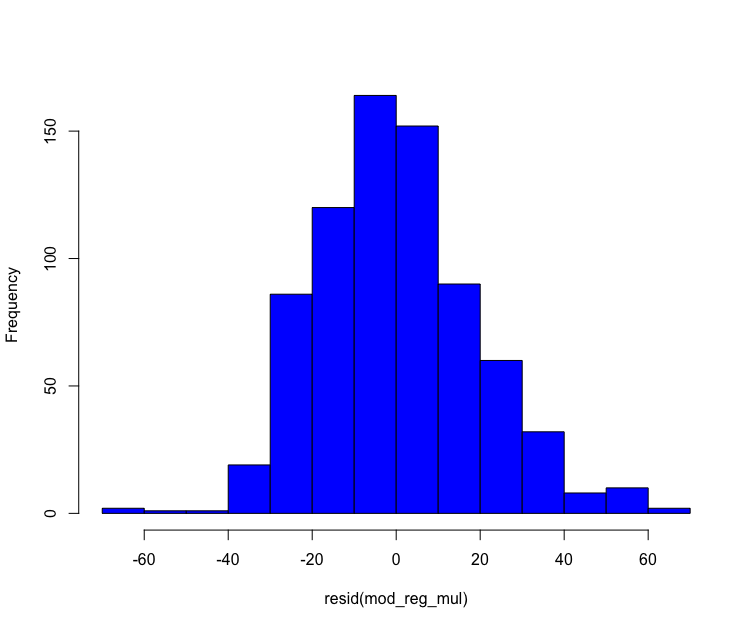
\includegraphics[scale=0.5]{ilu/cu.png}\end{center}\end{figure}

Nous obteenons donc un histogramme classique représentant le termer résiduel (le bruit) et l'on peut considérer graphiquement que les résidus du modèle suivent bien une loi normale.\newline 
\\
En conclusion, dans ce chapitre, nous avons étudié : 
\begin{itemize}
\item La régression linéaire multiple avec la fonction \textit{lm()} et la série de variables explicatives correspondante.
\item La possibilité d'ajouter une variable explicative catégorielle à plus de deux classes comme la variable profession et la nécessité de la recoder en une série de variables binaires.
\item La possibilité de changer la modalité de référence de ces variables catégorielles à plus de deux classes, ce qui facilite l'interprétation des résultats.
\item La fonction \textit{drop1()} qui permet d'avoir l'effet global de cette variable catégorielle à plus de deux classes.
\item  La notion d'interaction entre deux variables explicatives quand le modèle additif n?est potentiellement plus pertinent, avec le "multiplier" (x) que l'on met entre deux variables au lieu de les additionner.
\item La notion historique d'analyse de variance qui devrait être oubliée au dépend de la régression linéaire multiple, avec néanmoins la fameuse et classique analyse de variance à un facteur que l'on peut aussi réaliser à l'aide de la fonction \textit{lm()}.
\item Les conditions de validité de la régression linéaire multiple, difficile à apprécier, mais avec le minimum vital, l'appréciation de la normalité des résidus à l'aide des fonctions \textit{hist()} et \textit{resid()}.
\end{itemize}




\newpage

\section{Introduction à la régression logistique}
Après la régression linéaire, nous allons à présent nous intéresser à la regression logisitique.\newline
\\
La régression logistique est classiquement utilisée avec des variables binaires que l'on souhaite expliciter. Une telle situation peut être fréquemment rencontrée dans les sciences humaines et sociales ou encore en médecine; Par exemple, si l'on souhaite expliquer les variables \textit{être au chomage} (oui,non), \textit{être séparé} (oui,non) et \textit{avoir une maladie donnée} (oui,non).\newline
Dans ce chapitre, nous allons nous intéresser à la question du \textit{risque suicidaire en prison} du fait du haut taux de ce dernier dans le mileu carcéral. \newline
\\
Nous disposons d'une variable binaire : \textit{haut risque suicidaire} (codée en 0 et 1). Nous allons l'expliquer par une série de variables explicatives possibles, parmi lesquelles par exemple, \textit{la durée de la peine}, \textit{l'existence de mesures disciplinaires}, \textit{l'existence d'antécédents d'abus dans l'enfance}.\newline
Comme dans le chapitre sur la regression linéaire multiple, nous avons ici une intrication possible des variables explicatives. En effet, il est possible d'imaginer que la durée de la peine est corrélée à l'existence de mesures disciplinaires. Si l'on suppose une peine longue, le détenu peut avoir tendance à s'énerver et donc, recevoir des mesures disciplinaires. De la même façon, des abus dans l'enfance peuvent générer des troubles de la personnalité qui peuvent également conduire à des comportements violent et donc, à des mesures disciplinaires, \dots (\textit{On peut en trouver plein des comme ça})\newline
Lorsque l'on va tenter de trouver des associations entres ces variables explicatives et la variable que l'on souhaite expliciter (à savoir le risque suicidaire), il serait particulièrement utile de pouvoir démêler le rôle et l'impact de chacune de ces variables explicatives.\newline
\\
Une première approche consisterait à effectuer une regression linéaire multiple entre expliquant la \textit{durée de l'incarcération}, l'\textit{existence d'un abus} et de \textit{mesures disciplinaires}.\newline

$$y= a + b\times\textrm{durée} + c\times\textrm{discip } + d\times\textrm{ abus} + bruit$$
avec $y$, le haut risque suicidaire.\newline
\\
le problème que l'on rencontre avec cette équation, c'est que l'on conserve une variable résiduelle à savoir le \textbf{bruit} qui possède une distribution \textbf{Normale}. Potentiellement, la droite $y$ (équation ci dessus) varie entre $\pm \infty$ ce qui est incompatible dans le cadre de l'explicatiion d'une variable de type binaire ($0$ ou $1$).\newline 
\textcolor{red}{\textbf{De manière générale}}, la regression linéaire multiple n'est applicable que dans les cas où l'on souhaite expliquer des variables quantitatives puisque l'équation de regression qui en résultera sera une combinaison linéaire des variables explicatives et d'un terme de bruit.\newline
La régression linéaire multiple n'est donc pas la méthode la plus adequate pour expliquer des variables binaires.\newline 
\\
Les statisticiens ont trouvés une astuce : \textit{Transformer la variable que l'on souhaite expliquer grâce à la fonction \textbf{logarithmique}}.\newline
\\
En reprenant le modèle précédent et en replaçant la valeur de $y$ : 
$$\log\left[\frac{P(\textrm{HRsuicide} = 1)}{1-P(\textrm{HRsuicide} = 1)}\right] = a + b\times\textrm{durée} + c\times\textrm{discip } + d\times\textrm{ abus}$$
\textit{Et pourquoi donc ? } car, par axiome, une probabilité varie entre $[0,1]$ et donc, $\log\left[\frac{P(\textrm{HRsuicide} = 1)}{1-P(\textrm{HRsuicide} = 1)}\right]$ varie entre $]-\infty;+\infty[$ (C'est mathématique). La droite de régression linéaire peut donc être obtenue par combinaison de variables explicatives que l'on souhaite.\newline
\\
\textbf{Note : } Puisque l'on régresse une probabilité et non plus une variable, on suppose que le facteur \textit{bruit} du modèle est nul.\newline
\\
L'évaluation des coefficient $a,b,d$ et $d$ seront calculés par \textbf{R}.\newline
\\
Dans l'exemple suivant, nous allons déterminer l'influence de l'existence d'anthécendents d'abus par régression logistique pour expliquer les hauts risques de suicide.\newline
\\
Nous allons tout d'abord commencer par un modèle de régression logistique somple. Nous allons tenter d'expliquer la présence d'un risque suicidaire (\textit{rs}) en fonction de la variable explicative : présence d'antécédents d'abus dans l'enfance.\newline 
S l'on se réfaire à la formule montrée précédemment, on peut écrire : 

$$\log\left[\frac{P(\textrm{rs} = 1)}{1-P(\textrm{rs} = 1)}\right] = a + b\times\textrm{ abus}$$

La fonction dans le logiciel \textbf{R} qui permet d'estimer une telle régression logisitique est la fonction \textit{glm()}, accronyme de \textit{Generalized Lineal Model}.\newline
La syntaxe de cette fonction est très proche de celle que nous avons déjà utilisé pour la fonction \textit{lm()}. 
\begin{center}
\textit{variable étudié $\sim$ variable explicative 1 + variable explicative 2 + \dots }
\end{center}
On doit de plus définir le type de variable explicative que l'on souhaite traiter. Dans notre cas, il s'agit d'une variable binomiale (succès/échecs, oui/non, 0/1, ...). Ainsi, nous ajoutons \textit{family="binomial"}.

\begin{lstlisting}[language=html]
> setwd("~/Desktop/DIVERS_TEMPLATES/R/TP")
> smp <-read.csv2("DONNEES/smp2.csv")
> mod <- glm(suicide.hr~abus, data = smp, family="binomial")
> summary(mod)

Call:
glm(formula = suicide.hr ~ abus, family = "binomial", data = smp)

Deviance Residuals: 
    Min       1Q   Median       3Q      Max  
-0.8446  -0.6020  -0.6020  -0.6020   1.8959  

Coefficients:
            Estimate Std. Error z value Pr(>|z|)    
(Intercept)  -1.6161     0.1154 -14.003  < 2e-16 ***
abus          0.7688     0.1897   4.052 5.07e-05 ***
---
Signif. codes:  0 ?***? 0.001 ?**? 0.01 ?*? 0.05 ?.? 0.1 ? ? 1

(Dispersion parameter for binomial family taken to be 1)

    Null deviance: 760.21  on 752  degrees of freedom
Residual deviance: 744.26  on 751  degrees of freedom
  (46 observations deleted due to missingness)
AIC: 748.26

Number of Fisher Scoring iterations: 4
\end{lstlisting}

On peut ainsi observer que pour cette régression, la valeur de $p$ est de $5.10^{-5}$; On peut donc en déduire qu'avec un risque de $5\%$, il existe une association statistiquement signitificative entre les antécédents d'abus dans l'enfance et un haut risque suicidaire pour un détenu incarcéré.\newline
\\
Si l'on souhaite à présent étudier la valeur du coefficient $b$, nous devons étudier la ligne \textit{Estimate} (Car pour le moment, c'est pas très clair). Nous pouvons voir lire dans la console ci dessus que $b$ équivaut à $0.7688$. \textit{Mais qu'est ce que cela signifie ?}\newline
Nous savons que $b$, correspondant à l'existence d'abus pendant l'enfance, est une variable binaire (codée sur $0$,$1$). On peut donc recourir à la fonction $t \longrightarrow e^{t}$ pour analyser le résultat ($e^{0} = 1$,$ e^{1}= 2,72$). On peut se rappeler que c'est l'\textbf{Odds Ratio}\footnote{L?odds ratio (OR) est une mesure statistique exprimant le degré de dépendance entre des variables aléatoires qualitatives - CF Chapitres précédents} qui associe des variables explicative avec des variables à expliquer.\newline
\\
\textbf{Note : } On rappelle que :
$$\log(\exp(a))=a$$
Cette propriété permet de rétablir une valeur comprise entre $[-\infty,+\infty]$

\begin{lstlisting}[language=html]
> exp(0.7688)
[1] 2.157176
\end{lstlisting}

Si la variable à expliquer est suffisamment rare alors l'odds-ratio est voisin du risque relatif, ici, on a un odds-ratio de $2,15$, ce qui signifierait que des antécédents d'abus dans l'enfance multiplient par $2$ la probabilité d'être à haut risque suicidaire.\newline
\\
On obtient donc le modèle suivant : 

$$\log\left[\frac{P(\textrm{rs} = 1)}{1-P(\textrm{rs} = 1)}\right] = a + 0,7688 \times\textrm{ abus}$$

On peut vérifier la valeur de l'Odds Ratio en le calculant grâce à la fonction \textit{twoby2()} de la librairie $EPI$.

\begin{lstlisting}[language=html]
> library(Epi)
> twoby2(1-smp$suicide.hr, 1-smp$abus)
2 by 2 table analysis: 
------------------------------------------------------ 
Outcome   : 0 
Comparing : 0 vs. 1 

    0   1    P(0) 95\% conf. interval
0  63  90  0.4118    0.3366   0.4913
1 147 453  0.2450    0.2122   0.2810

                                   95\% conf. interval
             Relative Risk: 1.6807    1.3276   2.1276
         Sample Odds Ratio: 2.1571    1.4873   3.1287
Conditional MLE Odds Ratio: 2.1547    1.4577   3.1764
    Probability difference: 0.1668    0.0837   0.2525

             Exact P-value: 1e-04 
        Asymptotic P-value: 1e-04 
------------------------------------------------------
> exp(0.7688)
[1] 2.157176
\end{lstlisting}
Nous obtenons effectivement une valeur du Odds Ratio égale à $e^{0.7688} = 2.157176$.

\newpage

%%%%%%%%%%%%%%%%%%%%%%%%%%%%%%%%%%%%%%%%%%%%%%%%%%%%%%%%%%%%%%%%%%%%%%%%%%%%%%%%%%%%%%%%%%%%%%%%%%%%%%%%%%%%%%%%%%%%%%%%%%%%%%

\section{Régression logistique avec plusieurs variables explicatives}
Nous allons maintenant nous intéresser aux régressions logistiques pour des modèles comportant plusieurs variables explicatives.\newline
\\
Dans ce chapitre, nous allons nous poser la question suivante : \textit{Est-ce qu'un haut risque suicidaire en prison est associé à : 
\begin{enumerate}
\item à la durée d'incarcération
\item à des mesures disciplinaires
\item à des antécédents d'abus dans l'enfance
\end{enumerate}}
Pour ce faire, nous allons utiliser une régression logistique que l'on peut qualifier de multiple comme une regression linéaire multiple. Voici le modèle que nous allons étudier : 
$$\log\left[\frac{P(\textrm{HRsuicide} = 1)}{1-P(\textrm{HRsuicide} = 1)}\right] = a + b\times\textrm{durée} + c\times\textrm{discip } + d\times\textrm{ abus}$$
La fonction correspondante est la fonction \textit{glm()} avec la syntaxe suivante : 
\begin{itemize}
\item La variable à expliquer
\item Un tilde $\sim$
\item Les variables explicatives
\item Le nom du dataframe dans lequel nous trouvons les variables 
\item l'instruction \textit{family="binomial"} pour spécifier que nous allons réaliser une régression logistique
\end{itemize}
La ligne de commande est donc : 
\begin{lstlisting}[language=html]
smp <- read.csv2("smp2.csv")
mod_reg_log = glm(suicide.hr~abus+discip+duree,data= smp, family = "binomial")
\end{lstlisting}
Nous allons donc stocker le tout dans un objet et utiliser la fonction \textit{summary()}.\newline

\begin{lstlisting}[language=html]
> mod_reg_log = glm(suicide.hr~abus+discip+duree,data= smp, family = "binomial")
> summary(mod_reg_log)

Call:
glm(formula = suicide.hr ~ abus + discip + duree, family = "binomial", 
    data = smp)

Deviance Residuals: 
    Min       1Q   Median       3Q      Max  
-1.3200  -0.6655  -0.6012  -0.4997   2.0700  

Coefficients:
            Estimate Std. Error z value Pr(>|z|)    
(Intercept) -0.02462    0.49635  -0.050 0.960439    
abus         0.62289    0.22764   2.736 0.006213 ** 
discip       0.52809    0.23767   2.222 0.026287 *  
duree       -0.39862    0.11723  -3.400 0.000673 ***
---
Signif. codes:  0 ?***? 0.001 ?**? 0.01 ?*? 0.05 ?.? 0.1 ? ? 1

(Dispersion parameter for binomial family taken to be 1)

    Null deviance: 555.94  on 549  degrees of freedom
Residual deviance: 533.26  on 546  degrees of freedom
  (249 observations deleted due to missingness)
AIC: 541.26

Number of Fisher Scoring iterations: 4
\end{lstlisting}

on obtient ainsi les résultats suivant : 


\begin{center}
\begin{tabular}{c|c|c|}
\hline
 & \textbf{Estimate} & \textbf{Pr$(>|z|)$} \\ \hline
\multicolumn{1}{|c|}{\textbf{abus}}   & 0.62289           & 0.006213            \\ \hline
\multicolumn{1}{|c|}{\textbf{discip}} & 0.52809           & 0.026287            \\ \hline
\multicolumn{1}{|c|}{\textbf{duree}}  & -0.39862          & 0.000673            \\ \hline
\end{tabular}
\end{center}

Nous pouvons, dans un premier temps, regarder les valeurs de $p$ ($Pr(>|z|)$) et on remarque que ces dernières sont toutes inférieures à $5\%$. On peut donc en déduire que ces trois variables explicatives sont statistiquement associées à un haut risque suicidaire, et ce, toutes choses égales et par ailleurs (\textit{ceteris paribus}), en tout cas "toutes choses", tous paramètres mesurées et inclus dans le modèle, plus précisement.\newline
\begin{itemize}
\item Des antécédents d'abus dans l'enfance sont statistiquement associés à un haut risque suicidaire, et cen à mesures disciplinaires éventuelles constantes et à durée d'incarcération constante.
\item La durée d'incarcération est statistiquement associée au risque suicidaire et ce, même compte tenu d'éventuelles mesures disciplinaires et d'un éventuel antécédent d'abus dans l'enfance.
\end{itemize}

Le modèle obtenu est donc le suivant : 

$$\log\left[\frac{P(\textrm{HRsuicide} = 1)}{1-P(\textrm{HRsuicide} = 1)}\right] =  -0.02+ 0.63\times\textrm{durée} + 0.53\times\textrm{discip } -0.40 \times\textrm{ abus}$$

Si nous nous intéressons plus en détail aux coefficients de la colonne \textit{Estimate} et que nous étudions leurs signes, nous pouvons interpréter ce signe en fonction du codage des variables explicatives. \newline
Dans notre cas, le codage est le suivant : 
\begin{itemize}
\item $1$ pour abus, $0$ pour pas d'abus
\item $1$ pour mesures disciplinaires , $0$ pour absence de mesures disciplinaires
\item la variable durée, elle, est codée de 1 à 5 ; plus la variable est élevée, plus la durée d'incarcération est longue.
\end{itemize}
Autrement dit, ces trois variables sont codées de la manière suivante : plus elles sont élevées, plus le niveau d'exposition, le niveau du risque est élevé. \newline 
Théoriquement, si ces trois variables sont des facteurs de risque, nous devrions avoir une augmentation du risque correspondant et donc des coefficients positifs.\newline
On peut observer que c'est bien le cas pour les variables explicatives représentant l'abus et les mesures disciplinaires mais, que c'est le contraire pour la variables correspondant à la durée.\newline
Dans les faits et contrairement à ce que l'on aurait pu penser, une durée d'incarcération élevée diminue la probabilité d'être à haut risque suicidaire. 
Nous venons donc de réaliser l'analyse du signe des coefficients du modèle de régression logistique; étape \textcolor{red}{très importante}.\newline
\\
Nous pouvons maintenant tenter d'interpréter l'amplitude des coefficients et n'oubliant pas que sous cette forme, ces derniers ne sont pas interprétables (Nous sommes dans une expression logarithmique). Nous devons donc appliquer l'instruction \textit{exp()} sur les coefficients, récupérés grâce à la fonction \textit{coefficients()}.
\begin{lstlisting}[language=html]
> exp(coefficients(mod_reg_log))
(Intercept)        abus      discip       duree 
  0.9756803   1.8643147   1.6956873   0.6712485 
\end{lstlisting}
Nous obtenons ainsi des résultats autour de $1,9$ et $1,7$. Nous pouvons ainsi en déduire que l'existence d'antécédents d'abus dans l'enfance multiplie quasiment par $2$ le risque de présenter de haut risque suicidaire en prison et ceci, indépendamment de l'existence de mesures disciplinaireset de la durée d'incarcération.\newline
Concernant la durée d'incarcération, cette dernière n'est pas binaire (codée sur 0 et 1). La question qui se pose alors est de savoir comment interpréter le coefficients $0,7$. Il s'agit en fait du coefficient multiplicateur entre deux changement de modalité dans la variable durée. \newline
Si l'on considère le codage de la variable durée suivant : la durée d'incarcération définie par $1$ correspond à moins de 1 mois de détention; par 2, de 1 à 6 mois; par 3 : de 6 mois à 1 an; par 4, de 1 à 5 ans et par 5, plus de 5 ans.\newline
Lorsque l'on passe d'une modalité vers une modalité supérieure, le niveau de haut risque suicide diminue d'environ $(1-0,7) = 0,3$ soit $30\%$ ($0,3$ étant le complément de l'Odds-Ratio que l'on a ici, voisin de $0,7$).\newline
\\
Dans le cadre d'une régression logistique à plusieurs variables, on peut retrouver certaines similitudes avec une régression linéaire multiple : Par exemple, il est possible d'insérer dans le modèle, des variables catégoricielles à plus de deux classes; \textbf{R} recodera automatiquement ces dernières en $k-1$ variables binaires (en supposant que l'on a initialement $k$ modalités dans la variable catégoricielle). Nous aurons ainsi $k-1$ valeurs de $p$ et des coefficnets qui seront à interpréter par rapport à une modalité de référence (que l'on pourra également changer).\newline
De plus, si nous souhaitons analyser l'effet global de la variable catégoricielle sur la variable que l'on souhaite étudier, nous utiliserons également la fonction \textit{drop1()} avec la même syntaxe sauf que cette fois ci, nous écrirons \textit{\textcolor{red}{test="Chisq"}} à la place de \textit{test="F"}.\newline
De la même manière, il est aussi possible d'essayer de trouver des synergies entre des variables explicatives, c'est à dire mettre des termes en interaction. Par exemple, nous avons vu précédemment que la durée d'incarcération et les mesures disciplinaires étaient des facteurs de risque suicidaire. Nous pouvons imaginer qu'un détention, au début de sa peine c'est à dire, au moment ou les risque suicidaire est important, se voit imposer une mesure disciplinaire. On peut imaginer que les deux facteurs de risque génèrent un risque qui peut être beaucoup plus important que la sommation simple des deux risques. Il y aurait donc une synergie entre les facteurs de risque. Il fautdrait alors introduire un terme d'interaction, qui serait quant à lui, caractérisé par le produit des deux variables et nous interpréterions les résultats de la même manière que dans le chapitre sur les régressions linéaires multiples.\newline
\\
Intéressons nous maintenant aux conditions de validité d'une régression logistique. Ces dernières sont encore plus compliquées que celles pour une régression linéaire.\newline
Pour simplifier l'ensemble des conditions de validité et aller à l'essentiel, on pourra se souvenir qu'il faut au minimum entre $5$ et $10$ évènements par variable explicative.\newline
Dans le dataframe \textit{santé mentale en prison}, nous avons $799$ détenus.

\begin{lstlisting}[language=html]
> table(smp$scz.cons)

  0   1 
733  66 
\end{lstlisting}
Si l'on s'intéresse à la variable explicative \textit{schizophrénie consensuelle (scz.cons)} caractérisant les détenus avec une forme grave de schizophrénie, nous en avons alors 66.\newline
Dès lors, imaginons que nous cherchions à expliquer ces troubles de la personnalité en fonction de l'âge, d'existence d'un trauma durant l'enfance et de la profession. Nous réaliserions alors un modèle de régression logistique à trois variables.\newline
les variables \textit{age} et \textit{abus} sont des variables binaires non recodées. Pour la variable \textit{profession}, c'est une variable explicative comportant 8 modalités, recodée en 7 variables binaires. Le modèle comporte donc $1+1+7 = 9$ variables binaires explicatives.\newline
Pour que la modèle de régression logistique soit valide, il faut entre $5$ et $10$ évènements par variable explicative.\newline
Prenons la contrainte la plus forte, à savoir $10$ évènements par variable explicative. Il faudrait donc $(1+1+7)\times 10 = 90$ détenus au minimum pour que la régression logistique soit valide; Or, nous n'en avons que $66$. Par cette première contrainte, on peut en déduire que ce modèle de régression logistique n'est pas pertinent.\newline
Prenons la contrainte la plus forte, à savoir $10$ évènements par variable explicative. Il faudrait donc $(1+1+7)\times 5 = 45$ détenus au minimum pour que la régression logistique soit valide; Or, nous avons $66$. Par cette seconde contrainte, on peut en déduire que ce modèle de régression logistique est pertinent.\newline
En conclusion, sous la contrainte n°$1$, il nous faudrait au minimum $90$ détenus atteints de schizophrénie pour expliquer ce trouble par les variables \textit{age},\textit{abus} et \textit{profession} et sous la contrainte n°$2$, il nous faut au minimum $45$ détenus atteints de schizophrénie pour expliquer ce trouble par ces mêmes variables.

\newpage



%%%%%%%%%%%%%%%%%%%%%%%%%%%%%%%%%%%%%%%%%%%%%%%%%%%%%%%%%%%%%%%%%%%%%%%%%%%%%%%%%%%%%%%%%%%%%%%%%%%%%%%%%%%%%%%%%%%%%%%%%%%%%%

\section{Données censurées, survie : vocabulaire et approches descriptives}
Nous allons maintenant étudier des données censurées parmi lesquelles, la survie\footnote{L'analyse de (la) survie est une branche des statistiques qui cherche à modéliser le temps restant avant la mort pour des organismes biologiques (l'espérance de vie) ou le temps restant avant l'échec ou la panne dans les systèmes artificiels, ce que l'on représente graphiquement sous la forme d'une courbe de survie. } est un exemple classique.\newline
Nous allons tout d'abord nous focaliser sur le vocabulaire utilisé dans ce domaine et sur les approches statistiques descriptives qui lui sont propres.\newline
\\
Il n'est pas rare que des mesures effectuées dans des études correspondent à des durées. Ce sera par exemple le cas si l'on analyse un groupe de sujets au chômage que l'on aura suivi pendant un an. Durant cette période, nous aurons mesuré le temps jusqu'à recouvrement du travail.\newline
Cela pourra être également le cas si nous prenions en charge un groupe de patients ayant un infarctus du myocarde et que nous les suivions jusqu'à l'obtention d'une récidive ou du décès.\newline
Ces durées ont comme particularité qu'elles peuvent être potentiellement censurées.\newline
Qu'est ce qu'une \textit{statistique censurée} ? Dans le cas où nous avons la charge d'un groupe de sujets que nous avons suivi pendant un an, certains sujets vont avoir retrouvé du travail au bout de 2 mois, 4 mois, 6 mois \dots Pour ces sujets, on connait exactement la durée jusqu'au recouvrement de travail. Cependant pour d'autres membres du groupe, au bout d'un an, certains n'auront pas retrouvé de travail. Donc, le temps jusqu'à recouvrement du travail de certains individus ne sera pas connu par manque de suivi. Mais, on saura tout de même que le temps de recouvrement est supérieur à un an. Dans ce cas là, lorsque l'on a qu'une \textbf{connaissance partielle de la variable mesurée}, on dit qu'une \textbf{variable est censurée}.\newline 
\\
Les statisticiens ont développé de nombreuse méthodes spécifiquement adaptées à l'analyse des données censurées, ce que nous allons étudier dans ce chapitre.\newline 
\\
Nous pourrions nous dire que le changement de variable à étudier serait une bonne manière de ne pas avoir à étudier des données censurées. Par exemple, plutôt que d'étudier la variable \textit{durée jusqu'à survenue de l'évènement}, nous pourrions étudier la variable \textit{pourcentage de survenue de l'évènement}. On pourrait également étudier \textit{pourcentage de chômeur ayant retrouvé du travail en un an} plutôt que d'étudier \textit{durée jusqu'à recouvrement de travail}.\newline
Cependant, lorsque nous réalisons une étude, nous ne sommes jamais sûr de pouvoir suivre les sujets pendant la totalité de la période (par exemple, étude d'un groupe de personnes au chômage sur an). En effet, il est possible que l'inclusion (d'un individu dans le groupe) puisse durer longtemps et que nous n'avons pas le temps d'attendre un an une fois que les derniers sujets ont été inclus. il est également possible que certains sujets déménagent et, à ce moment là, soient perdus de vue.\newline
Si nous étudions le pourcentage de survenue de l'évènement à un an, tous ces sujets, nous serons obligés de les abandonner et cela peut induire des biais ou une perte de puissance.\newline
\\
Dans le domaine des données de survie, il existe un vocabulaire très spécifique que l'on doit connaitre.\newline
Le permier élément de langage est la notion même de \textbf{survie}. Largement abusive car en général, on ne s'intéresse pas aux décès des individus mais au délai jusqu'à survenue d'un évènement. Mais comme le délai de survie est effectivement le délai jusqu'a survenue d'un évènement (et là, nous parlons de la mort de cet individu), alors de façon métaphorique, nous parlons de données de survie bien qu'il s'agisse que d'un délai jusqu'à survenue d'un évènement et que ce dernier n'est en général pas la mort de cet individu.\newline
Le deuxième point est la notion de \textbf{censure}. Nous avons brièvement vu ce que ce terme signifiait mais sur un plan méthodologique, il est important de différencier deux types de censures : 
\begin{itemize}
\item Le premier correspond aux \textit{exclus vivants}. Nous devrions suivre les patients pendant une période (un an), nous les suivons sur toute cette période (un an) et à la fin de cette période (d'un an), certains individus sont vivants. On parle d'exclus vivants. 
\item Le second correspond aux \textit{perdus de vue}. Nous devrions suivre les patients pendant une période et puis, au bout de trois mois, le patient déménage. On dit alors que le patient est perdu de vue mais il n'a pas été suivi pendant un an. 
\end{itemize}

Ces deux types de censures sont différentes car il est tout à fait possible que des patients, perdus de vue, aient des biais\footnote{En statistique ou en épidémiologie, un biais est une démarche ou un procédé qui engendre des erreurs systématiques dans les résultats d'une étude.} qui soient différents que des exclus vivants. En effet, le fait qu'un patient déménage peut être possiblement lié au fait qu'il se trouve en bonne santé ou au contraire, en mauvaise santé, ce qui sera différent des exclus vivants. De là, la nécessité de bien différentier les deux types de censure.\newline
\\
Dans le cadre de l'analyse des données de survies, il faut également définir l'élément statistique suivant : \textit{la fonction de survie}\newline
Le terme de survie est également utilisé de manière abusive. En effet, la fonction de survie représente le pourcentage des sujets survivants au cours du temps ou, le pourcentage de sujets qui n'ont pas encore obtenu l'évènement au cours du temps. C'est une fonction nécéssairement décroissante qui part de $100\%$ (la totalité du groupe) à $0\%$ (si tous les membres du groupe décède un jour).\newline
Enfin, il faut également définir la notion de \textit{risque instantanté de décès} qui est une notion plus abstraite (car plus mathématique).\newline
Avec ce type de données, il serait intéressant de pouvoir décrire au cours du temps, l'évolution de la probabilité de décéder et ceci, à un instant donné. Cependant, la probabilité de décéder à un instant donné est $0$ (considérée comme l'évènement impossible); la probabilité de mourir un jour donné est un nombre \textit{petit} alors que la probabilité de mourir à une minute donnée est un nombre \textit{quasiment microscopique} qui n'a pas de sens.?newline
On ne peut donc pas représenter la fonction de risque instantanté de décès.\newline
Cependant, les mathématiciens ont développé grâce aux fonctions dérivées, une fonction que l'on appelle $h(t)$ qui permet d'obtenir une approximation d'une probabilité ponctuelle. $h(t)$ est alors appellé \textit{risque instantané de décès}.\newline
\\
Nous allons à présent voir comment représenter graphiquement la fonction de survie. Pour ce faire, nous allons prendre pour exemple un essai qui a étudié le premier médicament véritablement efficace dans le cadre du traitement de la leucémie.

\begin{figure}[H]\begin{center}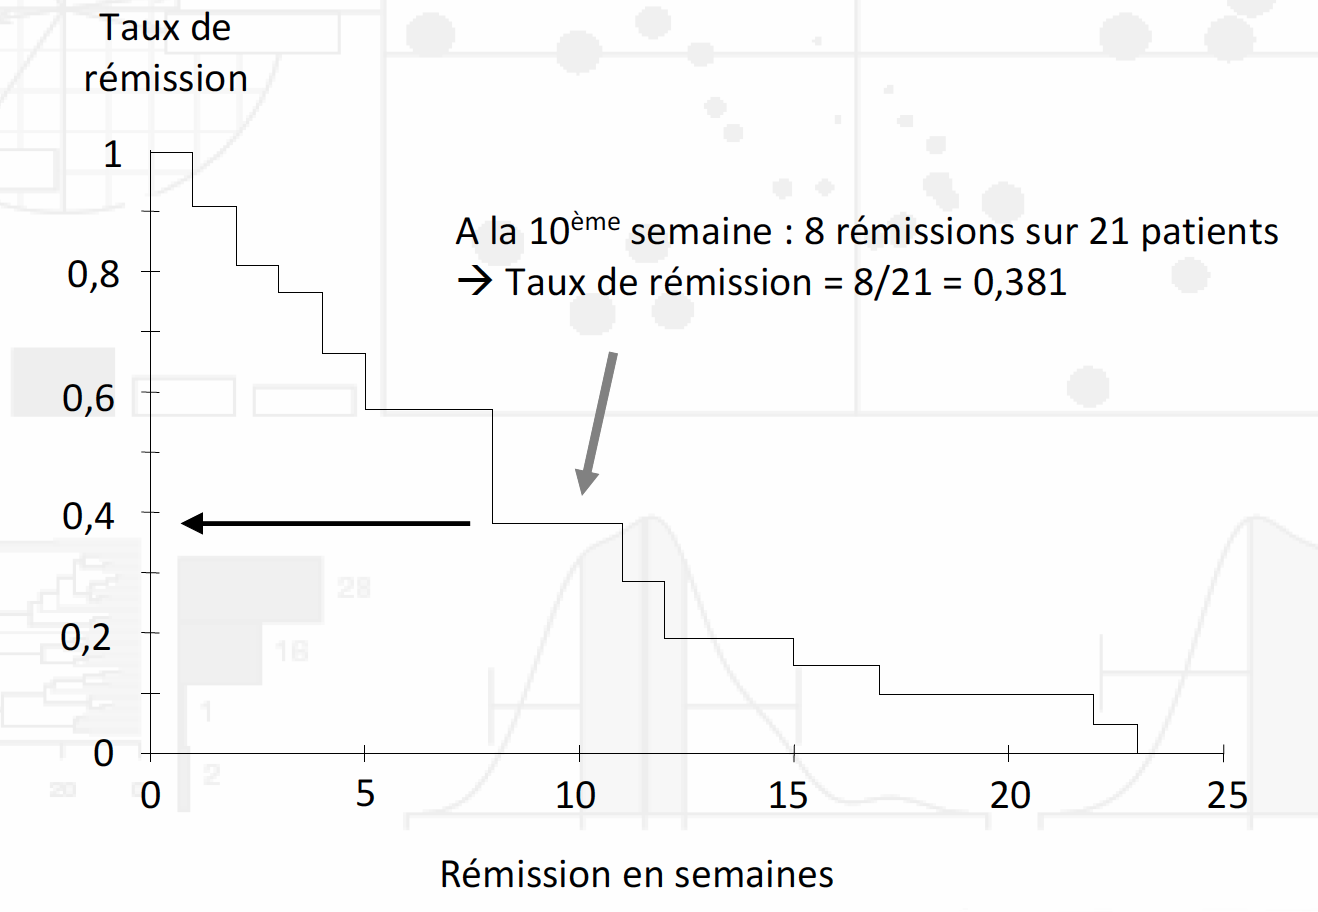
\includegraphics[scale=0.5]{ilu/dsurv1.png}\end{center}\end{figure}

Sur ce graphique, nous pouvons analyser le taux de rémission exprimé en semaine alors que l'on utilisait encore un traitement à base de corticoïdes. Ce dernier opérait quelques semaines mais il y avait très vite un échappement thérapeutique\footnote{l'échappement thérapeutique est le fait, pour un traitement, de devenir inefficace après une période d'efficacité.} au bout de $15$ à $20$ semaines et l'ensemble des patients mourraient.\newline
Dans ce cas, la fonction de survie est facilement représentable : Comme nous avons suivi les sujets jusqu'à leurs décès, nous pouvons calculer au fil du temps, le pourcentage de sujets survivants et l'on obtient le graphique ci-dessus.

\begin{figure}[H]\begin{center}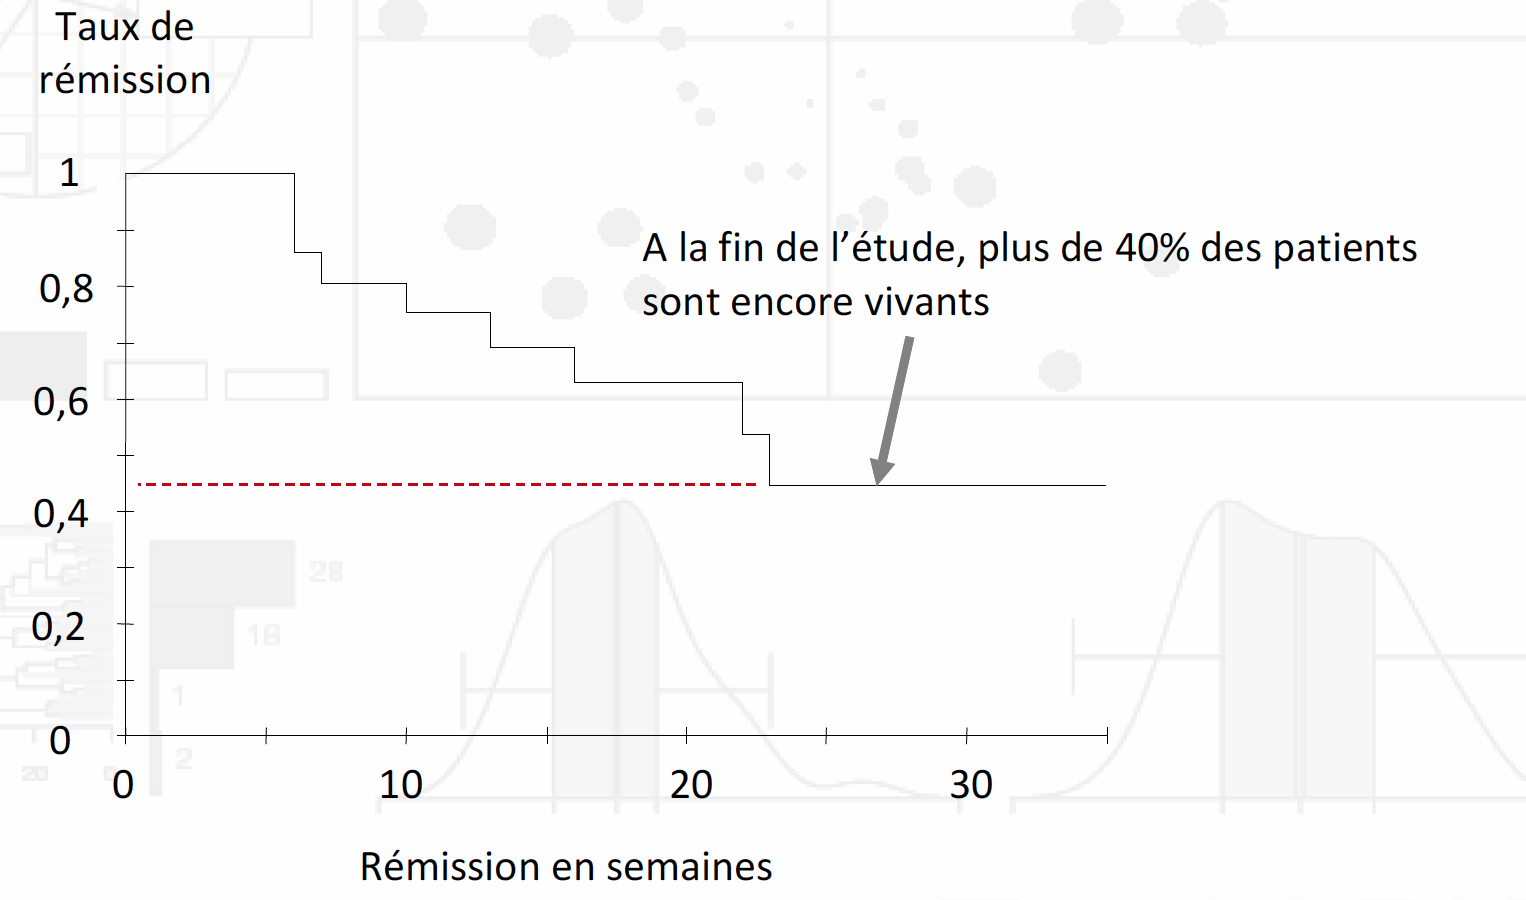
\includegraphics[scale=0.5]{ilu/dsurv2.png}\end{center}\end{figure}
Dans le cadre du second traitement, à la fin de l'essau et du suivi des patients, on peut observer que $40\%$ des sujets sont encore en vie. Il se pose  alors la question de la représentation de la fonction de survie.\newline
En effet, au fur et à mesure que le temps passe, le numérateur change car il correspond au nombre de sujets survivant mais de plus, le dénominateur change également car il représente le nombre de sujets encore vivants qui continuent a être observés. Cela devient donc délicat de calculer de manière non biaisée, avec un tel jeu de données, le pourcentage de survivants c'est à dire, la fonction de survie.\newline
Les statisticiens ont alors développé une méthode connue sous le nom de \textit{Méthode de Kaplan - Meier}.\newline
\\
Pour étudier la méthode de Kaplan - Meier à l'aide du logiciel \textbf{R}, nous allons nous intéresser à un nouveau dataset\footnote{l'étude santé mentale en
prison étant une étude transversale, nous n'avons pas de suivi de patients. Nous n'avons donc pas de durée jusqu'à survenue d'un évènement et donc pas de données censurées.}, cette fois ci composé de $125$ patients alcooliques qui ont été hospitalisés puis sevrés. Ces patients ont étés suivis et nous avons à notre disposition les $5$ variables suivantes : 
\begin{enumerate}
\item Le délai d'observation t
\item Le fait que les patients soient toujours sevrés à la fin de l'étude 
\begin{itemize}
\item $1$ : ils ont rechutés
\item $0$ : ils sont toujours sevrés
\end{itemize}
\item l'âge
\item Le sexe du patient 
\item L'existence d'un évènement de vie négative pendant le suivi 
\begin{itemize}
\item $1$ : Oui 
\item $0$ : Non 
\end{itemize}
\end{enumerate}

\begin{lstlisting}[language=html]
> alc <- read.csv2("DONNEES/alcool.csv")
> str(alc)
'data.frame': 125 obs. of  5 variables:
 $ t     : int  121 121 40 39 66 64 5 30 34 5 ...
 $ SEVRE : int  0 0 0 0 0 0 1 0 0 0 ...
 $ AGE   : int  53 52 45 48 45 42 35 35 41 37 ...
 $ SEXE  : int  1 2 2 1 1 1 1 1 1 1 ...
 $ EDVNEG: int  0 0 0 1 0 0 0 0 0 0 ...
\end{lstlisting}

Grâce à ce nouveau jeu de données, la variable censurée que nous allons étudier correspond au délai jusqu'à la survenue de l'évènement : \textit{"Rechute de la maladie alcoolique"}.\newline
\\
Pour tracer la fonction de survie de cette variable censurée, nous allons utiliser la librairie \textit{survival} qui contient l'ensemble des méthodes adaptées aux données censurées.\newline
\\
Nous allons utiliser trois fonction successivement : la fonction \textit{plot()}, la fonction \textit{survfit()}\footnote{This function creates survival curves from either a formula (e.g. the Kaplan-Meier), a previously fitted Cox model, or a previously fitted accelerated failure time model.} et la fonction \textit{Surv()}\footnote{Create a survival object, usually used as a response variable in a model formula. }. La syntaxe de est alors la suivante : 
\begin{itemize}
\item On met tout d'abord le délai de survi \textit{t}
\item Puis la variable survenue de l'évènement \textit{SERVE} (perte du sevrage)
\item puis $\sim 1$
\end{itemize}



\begin{lstlisting}[language=html]
library(survival)
plot(survfit(Surv(alc$t,alc$SEVRE)~1),main="Courbe de maintien de l'abstinence",xlab="Temps",ylab = "%")
\end{lstlisting}
Nous obtenons alors en trait plein, la fonction de survie et en trait pointillé, l'intervalle de confiance à $95\%$ de la fonction de survie. 

\begin{figure}[H]\begin{center}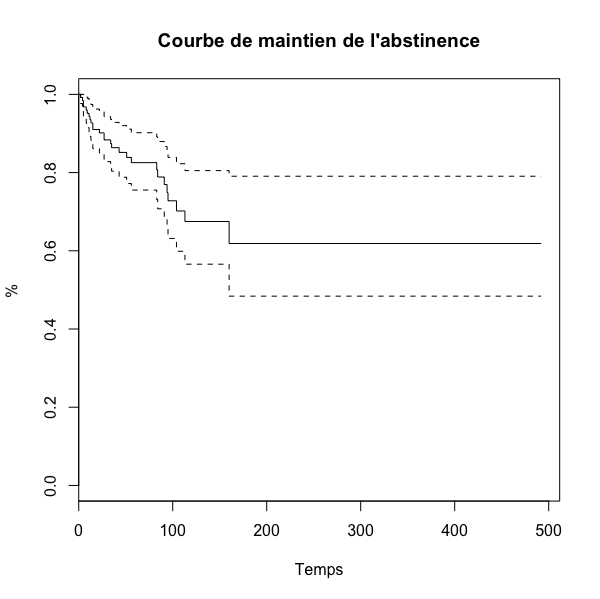
\includegraphics[scale=0.5]{ilu/dsurv3.png}\end{center}\end{figure}

En modifiant la syntaxe, on peut représenter graphiquement et sur un même schéma, plusieurs courbes de survie correspondant à la survie de diffrents groupes de sujets. Par exemple, si nous souhaitons représenter sur un même graphique, le temps jusqu'à la rechute de la maladie alcoolique chez les hommes et chez les femmes, il suffit alors de remplacer $\sim 1$ par $\sim SEXE$. Nous ajoutons également des couleurs afin de mettre avant le sexe du sujet : 

\begin{lstlisting}[language=html]
plot(survfit(Surv(alc$t,alc$SEVRE)~alc$SEXE),col=c("blue","red"),main="Courbe de maintien de l'abstinence",xlab="Temps",ylab = "%")
## Variante possible pour simplifier l'écriture : survfit(Surv(t,SEVRE)~SEXE,data=alc)
\end{lstlisting}

\begin{figure}[H]\begin{center}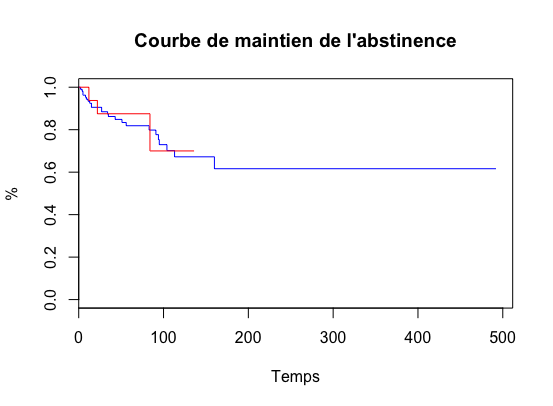
\includegraphics[scale=0.5]{ilu/dsurv4.png}\end{center}\end{figure}

Il existe des statistiques agrégées qui sont plus spécifiques à l'étude des données censurées. On peut par exemple évoquer la \textit{médiane de survie} qui correspond au moment où $50\%$ des sujets n'ont pas encore subit la survenue de l'évènement et $50\%$ des sujets l'ont subit.\newline
Pour obtenir ces données, il suffit juste de réutiliser la syntaxe que nous venons d'écrire en enlevant la fonction \textit{plot()} : 
\begin{itemize}
\item On met tout d'abord le délai de survi \textit{t}
\item Puis la variable survenue de l'évènement \textit{SERVE} (perte du sevrage)
\item puis $\sim 1$
\end{itemize}

\begin{lstlisting}[language=html]
survfit(Surv(t,SEVRE)~SEXE,data=alc)
Call: survfit(formula = Surv(t, SEVRE) ~ SEXE, data = alc)

         n events median 0.95LCL 0.95UCL
SEXE=1 107     24     NA     160      NA
SEXE=2  18      3     NA      84      NA
\end{lstlisting}
Dans notre cas, la médiane de survie n'est pas obtenue (on peut observer un NA qui correspond à une donnée manquante); Cela signifie tout simplement qu'à la fin de l'étude c'est à dire à la fin du delai de suivi, plus de $50\%$ des patients sont toujours sevrés et qu'il nous est donc impossible d'estimer une médiane de survie.

\newpage


%%%%%%%%%%%%%%%%%%%%%%%%%%%%%%%%%%%%%%%%%%%%%%%%%%%%%%%%%%%%%%%%%%%%%%%%%%%%%%%%%%%%%%%%%%%%%%%%%%%%%%%%%%%%%%%%%%%%%%%%%%%%%%


\section{Données censurées, survie : tests statistiques et modélisation}
Nous allons à présent nous intéresser aux tests statistiques et aux modèles multivariés que l'on peut réaliser sur des données censurées.\newline
\\
Dans le chapitre précédent, nous avons représenté sur un même graphique, les fonctions de survie relatives à la rechute de la maladie alcoolique chez un groupe de femmes et chez un groupe d'homme. 

\begin{figure}[H]\begin{center}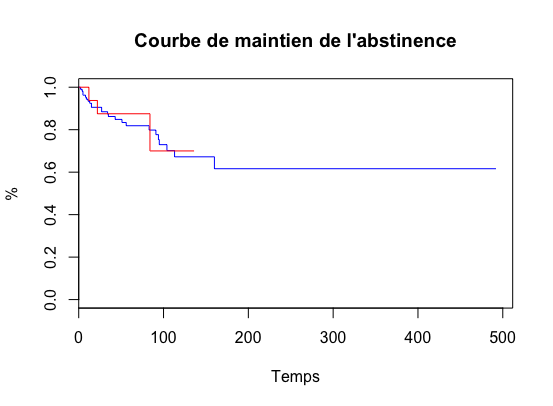
\includegraphics[scale=0.5]{ilu/dsurv4.png}\end{center}\end{figure}

On peut observer que les deux courbes ont l'air de se superposer. Mais on peut également se poser la question et tester statistiques si il existe une différence des taux de rechute entre les hommes et les femmes. Pour réaliser ce test, nous devons utiliser la méthode du \textit{Log-Rank}.\newline
\\
Le test du \textit{Log-Rank} est assimilé à un test de rangs; les rangs entre les temps de décès comme nous avons pu le voir dans le test de \textit{Wilcoxon}.\newline
Les conditions de validité de la méthode du Log-Rank sont plus délicates.\newline
La principale conditions de validité est la quantité de temps de décès. Si \underline{il y a de nombreux temps de décès, alors le test du Log-Rank est valide}.\newline
Dans le cadre de notre échantillon, si nous suivons des sujets et que nous effectuons des observations seulement tous les six mois, alors nous aurons peu de temps de décès mais il y aura beaucoup de décès sur chaque observations. Cette seconde configuration permet également d'assurer la validité du test du Log-Rank. Quand \underline{il y a de nombreux morts à chaque temps de décès, le test est également valide}.\newline
\\
Nous allons donc effectuer le test du Log-Rank sur notre jeu de donnée. La syntaxe est la suivante, nous allons utiliser la fonction \textit{survdiff()}\footnote{Tests if there is a difference between two or more survival curves using the G-rho family of tests, or for a single curve against a known alternative.} de la manière suivante :\textit{survdiff(Surv(délai,évènement)$\sim$classe)}

\begin{lstlisting}[language=html]
alc <- read.csv2("DONNEES/alcool.csv")
> survdiff(Surv(t,SEVRE)~SEXE,data=alc)
Call:
survdiff(formula = Surv(t, SEVRE) ~ SEXE, data = alc)

         N Observed Expected (O-E)^2/E (O-E)^2/V
SEXE=1 107       24    23.74   0.00281    0.0235
SEXE=2  18        3     3.26   0.02046    0.0235

 Chisq= 0  on 1 degrees of freedom, p= 0.878 
\end{lstlisting}
Les résultats obtenus sont alors très simple à interpréter. Sur la dernière ligne, on peut observer $p=0.87$; à l'évidence, il n'existe pas de différence statistique entre le pourcentage de rechite chez les hommes et chez les femmes. Cependant, on peut voir qu'il n'y a que $18$ femmes dans le dataset (\textit{SEXE=2}) sur $125$ observation. De plus, pour les femmes, on peut observer que \textit{Observed = 3} ce qui signifie que seulement $3$ rechutes ont été constatées chez les femmes.\newline
Ces échantillons étaient bien trop petit pour avoir une puissance suffisante afin de séparer les hommes des femmes.\newline
\\
Dans certaines situations, il serait potentiellement intéressant de tester l'association entre la survie et une variable quantitative. Dans noter exemple, nous pourrions tester l'association entre le risque de rechute de la maladie alcoolique et l'âge. On pourrait supposer que les sujets jeunes pourraient mal se connaitre, sous-estimer le risque de rechute et donc présenter des récidives plus précoces.\newline
Au contraire, on pourrait imaginer que les sujets âgés soient des patients chroniques enkystés\footnote{Qui se trouve enfermé dans un ensemble (Péjoratif). } dans leur maladie alcoolique et donc le risque de rechute pourrait être plus élevé.\newline
De toutes manière, la méthode statistique qui permet de tester une telle association est le \textit{Modèle de Cox}.\newline
Nous allons utiliser la fonction \textit{coxph()} et la syntaxe habituelle sur le délai de suivi \textit{t} et la variable de rechute \textit{SEVRE}.

\begin{lstlisting}[language=html]
> coxph(Surv(t,SEVRE)~AGE,data=alc)
Call:
coxph(formula = Surv(t, SEVRE) ~ AGE, data = alc)

       coef exp(coef) se(coef)     z     p
AGE -0.0467    0.9544   0.0235 -1.99 0.047

Likelihood ratio test=4.09  on 1 df, p=0.0431
n= 125, number of events= 27 
\end{lstlisting}
Les résultats sont eux aussi faciles à interpréter. Nous n'avons qu'une seule variable explicative : l'age.\newline
Au bout de la ligne, nous pouvons observer $p=0.047$. Cette valeur de $p-value$ est tout juste inférieure à $5\%$ mais au risque de $5\%$, on peut supposer qu'il existe une association entre l'âge et le risque de rechute de la maladie alcoolique.\newline
Pour interpréter le sens de cette association, nous devons regarder la valeur dans le colonne \textit{Coef}; nous obtenons alors $-0.0467$. Le signe de ce coefficient étant négative, on peut en déduire que la survenue d'une rechute alcoolique sera plus tardive pour les sujets plus âgés. L'âge à donc tendance à protéger les patients des rechutes dans la maladie alcoolique.\newline
Comme dans le cadre d'une régression linéaire multiple ou d'une régression logistique multiple, il est possible de tester l'association de la survie et d'une liste de variables explicatives. Ainsi, dans notre jeu de données, nous pourrions tester l'association entre le risque de rechute de la maladie alcoolique avec l'âge, le sexe et les évènements négatifs pendant le suivi. Nous obtiendrions ainsi, la force spécifique\footnote{A partir d'un ensemble de données,  on s'intéresse à une partie des données, par exemple, dans une enquête, à un sous-ensemble particulier des individus et/ou des variables. Comment analyser ce sous-ensemble, dans le contexte que constituent les autres données? En  langage sociologique,  si  les données d'ensemble définissent un champ (au sens de Bourdieu), une analyse spécifique sera l'étude d'un sous-champ.L'idée-force spécifique se rapporte à ce type de problèmes. Elle prend des formes différentes selon les situations.} de chaque variable explicative sur la variable à expliquer.\newline
Le modèle qui permet de tester une telle association est toujours le modèle de Cox.\newline
\\
La syntaxe à utiliser avec \textbf{R} est très semblable à la syntaxe utilisée dans les dernières diapositives : \textit{coxph(Surv())}, le délai, l'évènement et puis les trois variables explicatives AGE, SEXE, EDVNEG et puis enfin le nom du fichier.

\begin{lstlisting}[language=html]
> mod <- coxph(Surv(t,SEVRE)~AGE+SEXE+EDVNEG,data=alc)
> mod
Call:
coxph(formula = Surv(t, SEVRE) ~ AGE + SEXE + EDVNEG, data = alc)

          coef exp(coef) se(coef)     z     p
AGE    -0.0473    0.9538   0.0237 -2.00 0.046
SEXE   -0.0151    0.9850   0.6206 -0.02 0.981
EDVNEG -0.4428    0.6422   1.0240 -0.43 0.665

Likelihood ratio test=4.31  on 3 df, p=0.23
n= 125, number of events= 27 
\end{lstlisting}

Nous pouvons à présent observer trois lignes pour les variables explicatives et au bout de chaque lignes, les valeur de $p$. On peut ainsi en déduire qu'au risque de $5\%$, seul l'âge est statistiquement associé au risque de rechute avec cependant, une significativité limitée (trop proche des $5\%$).\newline
Le sexe et les évènements de vie négatifs ne sont donc pas statistiquement associés au risque de rechute de la maladie alcoolique (le sexe ayant pour $p-value = 0.981$ et l'existence d'évènements négatifs $p-value = 0.665$).\newline
Il est cependant possible de critiquer ces résultats. En effet, nous avons vu précédemment qu'il n'y avait que très peu de femme dans cet échantillon et donc très peu de puissance\footnote{En statistique, la puissance d'un test est la probabilité de rejeter l'hypothèse nulle (par exemple l'hypothèse selon laquelle les groupes sont identiques au regard d'une variable) sachant que l'hypothèse nulle est incorrecte. La puissance statistique consentie permet de calculer le nombre de sujets à inclure dans une étude. Le calcul de la puissance statistique peut s'appliquer à grand nombre de tests statistiques (comparaison de moyennes, comparaison de proportions, modèle logistique, modèle de régression?), lorsque l'hypothèse alternative est suffisamment restrictive.} dans le test d'association statistique. On peut également remarquer qu'il n'y a que $5$ sujets qui ont subis des éléments de vie négatifs, la puissance statistique d'association est donc très faible.\newline
Les tests statistiques qui nous conduisent à accepter l'hypothèse nulle sont donc à interpréter avec beaucoup de prudence. \newline
Quant à l'interprétation des coefficients, on peut observer qu'ils sont tous négatifs; On peut donc supposer qu'ils agissent dans le sens de la protection des sujets (plus on est agé, moins nous avons de risque de faire une rechute de la maladie alcoolique).\newline
Pour l'instant, les coefficients sont difficiles à interpréter en dehors de l'étude de signe. Le passage à l'exponentielle de ces coefficients peut cependant permettre d'améliorer l'interprétation des coefficients, notamment dans le cadre d'une explication à l'aide de variable explicative binaire.\newline

\begin{lstlisting}[language=html]
> exp(coef(mod))
      AGE      SEXE    EDVNEG 
0.9537763 0.9850037 0.6422475 
\end{lstlisting}

Parmi les résultats obtenus ci dessus, prenons comme exemple les évènements de vie négatifs. L'exponentielle du coefficient vaut $0.64$; on peut donc en déduire qu'il y a $1-0.64 = 36\%$ de chances de moins présenter un risque de rechute à un instant donné. La valeur $0.64$ est appelée \textit{Hazard Ratio} ou \textit{"Rapport des risques instantanés de décès"}. Comme nous l'avons évoqué précédemment, ce rapport de risques instantanés correspond au fait que l'on $1-0.64 = 36\%$ de change en moins de faire une rechute de la maladie alcoolique quand on a subi des évènements de vie négatifs plutôt que lorsque l'on en a eu (avec cette fois ci $64\%$ de chances).\newline
Dans cet exemple, les conclusions peuvent sembler paradoxales mais nous devons nous rappeler qu'il n'y a que $5$ individus sur les $125$ patients qui ont subis des évènements de vie négatifs et que la variable correspondante (\textit{EDVNEG}) n'est pas statistiquement associée à la rechute de la maladie alcoolique. L'interprétation de ce Hazard Ratio est donc à titre purement pédagogique.\newline 
\\
Nous allons à présent nous intéresser aux conditions de validité du modèle de Cox, qui, encore une fois, ne sont pas simples à vérifier.\newline
Tout d'abord, comme dans une régression logistique il faut que le modèle présente un nombre suffisant d'évènements, c'est à dire entre $5$ et $10$ par variable explicative.
Ensuite, la condition de validité propre au modèle de Cox est de vérifier \textit{l'hypothèse des risques instantanés proportionels}. Cette hypothèse se construit par la résolution de multiple équations (ce qui n'est pas l'objet de ce cours); mais heureusement, \textbf{R} permet de vérifier graphiquement l'hypothèse des risques instantanés proportionels grâce à la syntaxe suivante sur un modèle que l'on a estimé : 

\begin{lstlisting}[language=html]
mod <- coxph(Surv(t,SEVRE)~AGE+SEXE+EDVNEG,data=alc)
par(mfrow=c(2,2))
## Cette commande permet de réaliser plusieurs graphiques dans une même fenêtre -- Partition de la fenêtre en 2x2 celulles
plot(cox.zph(mod),col="red")
\end{lstlisting}

\begin{figure}[H]\begin{center}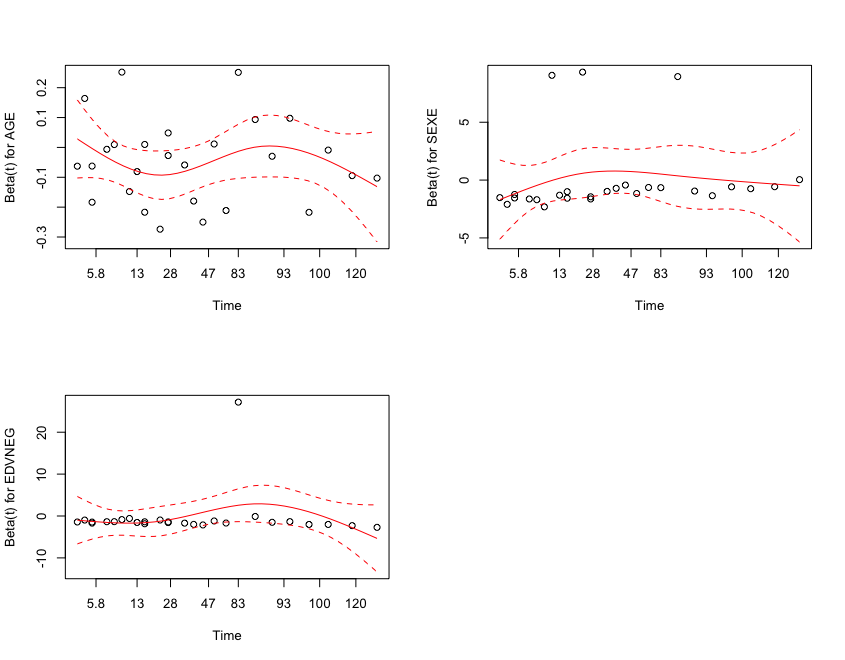
\includegraphics[scale=0.5]{ilu/dsurv5.png}\end{center}\end{figure}

\textbf{Note :} Pour les faire 1 par 1, on utilise la commande suivante : 
\begin{lstlisting}[language=html]
modAge <- coxph(Surv(t,SEVRE)~AGE,data=alc)
par(mfrow=c(1,1))
plot(cox.zph(modAge),col="red")
\end{lstlisting}

\begin{figure}[H]\begin{center}\includegraphics[scale=0.5]{ilu/dsurv6.png}\end{center}\end{figure}

\begin{figure}[H]\begin{center}\includegraphics[scale=0.5]{ilu/dsurv7.png}\end{center}\end{figure}

\begin{figure}[H]\begin{center}\includegraphics[scale=0.5]{ilu/dsurv8.png}\end{center}\end{figure}


Nous obtenons ainsi trois graphiques qui représentent les trois variables \textit{AGE}, \textit{SEXE} et \textit{EDVNEG}. Nous devons obtenir trois courbes en traits pleins le plus horizontal possible ce qui semble être le cas (mais vraiment à peu près) dans sur nos résultats. Donc, nous dirons, en première approximation, que l'hypothèse des risques instantanés proportionnels est vérifiée.\newline 
De plus, comme dans le chapitre sur la régression linéaire multiple et sur la régression logistique, nous pouvons inclure dans ces modèles des variables catégorielles à plus de deux classes qui seront recodées automatiquement en variables binaires et mettre des termes
d'interaction entre des variables pour rechercher les synergies entre variables explicatives.

\newpage
\section{Complément sur les données de survie}
\subsection{Introduction à l'analyse des durées de survie - Philippe SAINT PIERRE, Université Pierre et Marie Curie}
Le terme de durée de survie désigne le temps écoulé jusqu'à la survenue d'un événement précis. L'événement étudié (communément appelé décès) est le passage irréversible entre deux états (communément nommé vivant et décès). L'événement terminal n'est pas forcément la mort : il peut s'agir de l'apparition d'une maladie (par exemple, le temps avant une rechute ou un rejet de greffe), d'une guérison (temps entre le diagnostic et la guérison),la panne d'une machine (durée de fonctionnement d'une machine, en fiabilité) ou la survenue d'un sinistre (temps entre deux sinistres, en actuariat). [\dots]\newline
\\
Quelques définitions sont couramment utilisées dans les études de survie.
\begin{itemize}
\item Date d'origine : elle correspond à l'origine de la durée étudiée. Elle peut être la date
de naissance, le début d'une exposition à un facteur de risque, la date d'une opération
chirurgicale, la date de début d'une maladie ou la date d'entrée dans l'étude. Chaque
individu peut donc avoir une date d'origine différente (pas important car c'est la durée
qui nous intéresse).
\item Date de point : c'est la date au-delà de laquelle on arrêtera l'étude et on ne tiendra
plus compte des informations sur les sujets.
\item Date des dernières nouvelles : c'est la date la plus récente où des informations sur un
sujet ont été recueillies.
\end{itemize}
\textbf{Distributions de la durée de survie}\newline
Supposons que la durée de survie $X$ soit une variable positive ou nulle et absolument continue; alors sa loi de probabilité peut être définie par l'une des cinq fonctions équivalentes suivantes :\newline
\textit{Fonction de survie $S$} : La fonction de survie est, pour $t$ fixé, la probabilité de survivre jusqu'à l'instant $t$, c'est-à-dire : 
$$S(t) = \mathbb{P}(X > t), \textrm{ avec } t \geq 0$$
\textit{Fonction de répartition $S$} : La fonction de répartition (ou c.d.f. pour "cumulative distribution function") représente, pour $t$ fixé, la probabilité de mourir avant l'instant $t$, c'est-à-dire :
$$F(t) = \mathbb{P}(X \leq t) = 1 - S(t)$$
\underline{Remarque : } Il est arbitraire de décider que $S(t) = \mathbb{P}(X \geq t)$ ou $S(t) = \mathbb{P}(X > t)$. Cela n'a aucune importance quand la loi de X est continue car $\mathbb{P}(X > t) = P(X \geq t)$ : Dans les cas où $F$ a des sauts (quand le temps est discret, par exemple, compté en mois ou semaine), on utilise les notations suivantes :
$$F^{-}(t) = P(X < t) \textrm{ et } F^{+}(t) = P(X \leq t)$$
où $F^{-}$ est la limite à gauche et $F^{+}$ la limite à droite de $F$ (définitions et notations sont identiques pour la fonction $S$) : Remarquons que $F^{-} \leq F^{+}$ et $S^{-} \geq S^{+}$.\newline
\textbf{Densité de probabilité $f$} : C'est la fonction $f(t) \geq 0$ telle que pour tout $t > 0$ :
$$F(t) = \int_{0}^{t} f(u)\textrm{du}$$
Si la fonction de répartition $F$ admet une dérivée au point $f$ alors 
$$f(t) = \lim\limits_{h \rightarrow 0} \frac{\mathbb{P}(t\leq X < t+h)}{h} = F^{'}(t) = - S^{'}(t)$$
Pour $t$ fixé, la densité de probabilité représente la probabilité de mourir dans un petit intervalle de temps après l'instant $t$.\newline
\textit{Risque instantané $\lambda$ (ou taux de hasard)}\newline
Le risque instantané (ou taux d'incidence), pour $t$ fixé caractérise la probabilité de mourir dans un petit intervalle de temps après $t$, conditionnellement au fait d'avoir survécu jusqu'au temps $t$ (c'est-à-dire le risque de mort instantané pour ceux qui ont survécu) :
$$\lambda(t) = \lim\limits_{h \rightarrow 0} \frac{\mathbb{P}(t\leq X < t+h| X \geq t)}{h}  = \frac{f(t)}{S(t)} = - \ln(S(t))^{'}$$
\textit{Taux de hasard cumulé $\Lambda$} : Le taux de hasard cumulé est l'intégrale du risque instantané $\lambda$ :
$$ \Lambda(t) = \int_{0}^{t}\lambda(u)\textrm{du } = -\ln(S(t))$$
On peut déduire de cette équation une expression de la fonction de survie en fonction du taux de hasard cumulé (ou du risque instantané) :
$$S(t) = e^{-\Lambda(t)} = e^{\left( -\int_{0}^{t} \lambda(u)\textrm{du} \right)}$$
On en déduit que 
$$f(t) = \lambda(t)e^{\left( -\int_{0}^{t} \lambda(u)\textrm{du} \right)}$$
\textbf{Moyenne et variance de la durée de survie} : Le temps moyen de survie $\mathbb{E}(X)$ et la variance de la durée de survie $\mathbb{V}(X)$ sont définis par les quantités suivantes (en utilisant des IPP\footnote{Intégration par parties}) :
$$\mathbb{E}(X) = \int_{0}^{\infty} S(t)\textrm{ dt}$$
$$\mathbb{V}(X) = 2\int_{0}^{\infty} tS(t)\textrm{ dt} - (\mathbb{E}(X))^{2}$$
Ainsi on peut déduire l'espérance et la variance à partir de n'importe laquelle des fonctions $F, S, f, \lambda, \Lambda$ (mais pas l'inverse).\newline
\textbf{Estimateur de Kaplan-Meier de la survie} : L'estimateur de Kaplan-Meier découle de l'idée suivante : survivre après un temps $t$ c'est
être en vie juste avant $t$ et ne pas mourir au temps $t$; c'est-à-dire, si $t^{''} < t^{'} < t$ : 
$$\begin{aligned}
P(X > t) &= P(X>t', X > t) \\
        &= P(X > t | X > t')\times P(X > t') \\
        &= P(X > t | X > t') \times P(X > t' | X > t'') \times P(X > t'')
\end{aligned}$$
En considérant les temps d'événements (décès et censure) distincts $T_{(i)}$ avec  $(i = 1,  \dots , n)$ rangés par ordre croissant, on obtient :
$$P(X > T_{(j)}) = \prod_{k=1}^{j} P(X>T_{(k)} | X>T_{(k-1)})$$
avec $T_{(0)} = 0$, Considérons les notations suivantes :
\begin{itemize}
\item $Y_{i}$, le nombre d'individus à risque de subir l'événement juste avant le temps $T_{(i)}$.
\item $d_{i}$, le nombre de décès en $T_{(i)}$
\end{itemize}
Alors la probabilité pi de mourir dans l'intervalle $]T_{(i-1)},T_{(i)}$sachant que l'on était vivant en $T_{(i-1)}$, i:e: $p_{i} = P(X \leq T_{(i)}| X > T_{(i-1)})$, peut être estimée par
$$\widehat{p}_{i} = \frac{d_{i}}{Y_{i}}$$\footnote{$\widehat{p}$ ou $p$ chapeau est l'estimation de la probabilité $p$ par une certaine méthode d'approximation algébrique qui peut être le maximum de vraisemblance ou les moindres carrés utilisées en statistique. En pratique on donne une distribution statistique (ensemble de données chiffrées) et on essaie d'ajuster une fonction $\widehat{p}$ sur cette distribution.}
Comme les temps d'événements sont supposés distincts, on a :
\begin{itemize}
\item $d_{i} = 0 $en cas de censure en $T_{(i)}$, i.e. quand $\delta_{i} = 0$\footnote{$\delta_{i}$ est un indicateur tel que $\delta_{i} = \mathbb{1}_{\{X_{i}\leq C_{i}\}}$.\begin{itemize}\item $\delta_{i}=1$ si l'événement est observé (d'où $T_{i} = X_{i}$). On observe les "vraies" durées ou les durées complètes.\item $\delta_{i}=0$ si l'individu est censuré (d'où $T_{i} = C_{i}$). On observe des durées incomplètes (censurées).\end{itemize}};
\item $d_{i} = 1 $ en cas de décès en $T_{(i)}$, i.e. quand $\delta_{i} = 1$;
\end{itemize}
On obtient alors l'estimateur\footnote{un estimateur est une statistique permettant d'évaluer un paramètre inconnu relatif à une loi de probabilité (comme son espérance ou sa variance). Il peut par exemple servir à estimer certaines caractéristiques d'une population totale à partir de données obtenues sur un échantillon comme lors d'un sondage. La définition et l'utilisation de tels estimateurs constitue la statistique inférentielle.} de Kaplan-Meier :


$$\widehat{S}(t) = \prod_{i = 1,\dots,n\\T_{(i)}\leq t} \left( 1 - \frac{\delta_{i}}{Y_{i}} \right) = \prod_{i = 1,\dots,n\\T_{(i)}\leq t} \left( 1 - \frac{\delta_{i}}{n-(i-1)} \right) = \prod_{i = 1,\dots,n\\T_{(i)}\leq t} \left( \frac{n-i}{n-(i-1)} \right)^{\delta_{i}}$$

L'estimateur $\widehat{S}(t)$ est également appelé Produit Limite car il s'obtient comme la limite d'un produit. On montre que l'estimateur de Kaplan-Meier est un estimateur du maximum de vraisemblance. $\widehat{S}(t)$ est une fonction en escalier décroissante, continue à droite. On peut également obtenir un estimateur de Kaplan-Meier dans le cas de données tronquées mais pas dans le cas de données censurées par intervalles (car les temps de décès ne sont pas connus).\newline
\textbf{Type de censure}
La censure aléatoire est la plus courante. Par exemple, lors d'un essai thérapeutique, elle peut être engendrée par
\begin{itemize}
\item la perte de vue : le patient quitte l'étude en cours et on ne le revoit plus (à cause d'un déménagement, le patient décide de se faire soigner ailleurs). Ce sont des patients "perdus de vue".
\item l'arrêt ou le changement du traitement : les effets secondaires ou l'inefficacité du traitement peuvent entraîner un changement ou un arrêt du traitement. Ces patients sont exclus de l'étude.
\item la finn de l'étude : l'étude se termine alors que certains patients sont toujours vivants (ils n'ont pas subi l'événement). Ce sont des patients "exclus-vivants". Les "perdus de vue" (et les exclusions) et les "exclus-vivants" correspondent à des observations censurées mais les deux mécanismes sont de nature différente (la censure peut être informative chez les "perdus de vue").
\end{itemize}
\subsection{Institut de l'élevage - Séminaire d'épidémiologie animale - 28-30/09/2011}
\textbf{Terminologie}
\begin{itemize}
\item \textbf{Date d'origine (do)} : date d'entrée dans l'étude (peut être spécifique à l'individu)
\item \textbf{Date de point (dp)} : Date de fin de la période d'étude 
\item \textbf{Date des dernières nouvelles (ddn)} : Date la plus récente de recueil d'information sur un individu $i$
\item \textbf{Durée de surveillance (ds)} : délai écoulé entre la date d'origine et la date des dernières nouvelles
\item \textbf{Temps de participation (tp)} : 
\begin{itemize}
\item Si ddn $\leq$ dp, alors tp = ddn - do
\item Si dp $<$ ddn; alors tp = dp - do
\end{itemize}
\item \textbf{Censures} : 
\begin{itemize}
\item \textit{Perdu de vue} : Individu dont on ne connait pas l'état à la date de point
\item \textit{Exclu-vivant} : Individu vivant à la date de point
\end{itemize}
\end{itemize}
\textbf{Les différents types de censures}\newline
\textit{Les censures par intervalle : } Observation périodique des individus pendant toute la durée de l'étude. Exemple : Examen des animaux dans les élevages périodiques, passage tous les six mois.
La seule information disponible est que les événements se sont produits entre deux passages $t_{i}$ et $t_{i+1}$.\newline
\textit{Censure à gauche :} L'évenement s'est déja produit avant la premiere observation. L'individu est généralement exclu de l'analyse.\newline
\textit{Troncature : } Des "trous" dans le suivi des individus pendant lesquels on ne dispose d'aucune information, ni sur l'événement considéré ni sur les facteurs de risque potentiels. Impossible avec des événements "définitifs" (la mort).Trous en début de période : "Troncature a gauche" ; "troncature a droite" = censure à droite.\newline
\\
\textbf{Deux types de censures}\newline
\textit{Les censures non aléatoires} : Exemple, expérience carcinogène\footnote{Qui peut provoquer un cancer.} chimique :
\begin{itemize}
\item Suivi pendant quatre mois de n portées de rats traités.
\item Traitement d'une portée de rats parjour
\item Sacrifice des survivants au bout de quatre mois (censure à droite)
\item \textbf{Pas de perdus de vue}
\end{itemize}
\textit{Les censures aléatoires} Entrée aléatoire des individus dans l'étude. Exemple : Enquêtes sur population ouvertes, essai cliniques, \dots.
\textbf{La variable analysée}\newline
\begin{itemize}
\item $T_{i}$ : Temps au bout duquel apparaît l'évènement (échec, décès) pour un individu $i$. C'est le \underline{Temps de survie}.
\item $tp$ : \underline{Temps de participation}; Délai entre la date d'origine $\inf$(Date de dernière nouvelle, Date de point).
\end{itemize}
On peut représenter les observations pour un individu $i$ par le couple $(t_{i},\delta_{i})$ avec : 
\begin{itemize}
\item $t_{i} = \min(T_{i}, tp_{i})$
\item $\delta_{i} = 1$ si $T_{i}\leq tp_{i}$ (évènement "mort"); $\delta_{i} = 0$ si $T_{i} > tp_{i}$ (censure)
\end{itemize}
Le temps $T_{i}$ est considéré a priori comme continu.\newline
\\
\textbf{Une hypothèse fondamentale sur les censures (cas de censures aléatoires)}\newline
Il faut supposer que la durée de surveillance $ds$ et le temps au bout duquel se produit l'événement $T$ sont des variables indépendantes.\newline
\textit{Censure non informative"} Cela signifie que les perdus de vus ne le sont pas pour des raisons liées à l'événement étudié. C'est une condition nécessaire pour que les censures ne biaisent pas les résultats (et aussi pour que la vraisemblance ne soit pas fonction des temps de censure).\newline
Les censures non aléatoires ne posent pas de problèmes
\textbf{Les fonctions de survie }\newline
$T$ : \underline{Temps de survie}, est le temps au bout duquel se produit un certain évènement. Pour $t$ donné, la survie à $t$ est la probabilité que le temps de survie $T$ soit supérieur à $t$.
$$S(t) = \mathbb{P}(X > t), \textrm{ avec } t \geq 0$$
On désigne par $f(t)$, la densité de probabilité que l'évènement se produise à $t$ : 
$$f(t) = \lim\limits_{h \rightarrow 0} \frac{\mathbb{P}(t\leq X < t+h)}{h}$$
\underline{Le risque instantané} : Probabilité de mourir entre $t$ et $t+textrm{dt}$ sachant que l'individu est vivant avant $t$. On diminue l'intervalle jusqu'à le rendre infiniment petit $textrm{dt} \rightarrow 0$. On obtient alors le risque instantané de mort à $t$ : $h(t)$.\newline
\underline{Force de mortalité} $h(t)$ aussi appelée hazard\footnote{Hazard signifie risque en anglais et non hasard} function ou fonction de risque.
\underline{La fonction de risque cumulée} $H(t)$ (Cumulative Hazard Function) est le cumul des risques instantanés $h(t)$ sur une période données. 
$$H(t) = \int_{0}^{t} h(u)\textrm{ du}$$
$$S(t) = e^{-H(t)}$$
La probabilité de mourir dans l'intervalle $[0,t]$ est donc : 
$$P(t) = 1 - e^{-H(t)}$$
\textbf{L'estimation de la fonction de survie }
Il existe deux méthodes simples. Ce sont des méthodes non-paramétriques\footnote{Les tests paramétriques se basent sur des distributions statistiques supposées dans les données. Par conséquent, certaines conditions de validité doivent être vérifiées pour que le résultat d'un test paramétrique soit fiable. Par exemple, le test t de Student pour échantillons indépendants n'est fiable que si les données associées à chaque échantillon suivent une distribution normale et si les variances des échantillons sont homogènes.\newline
Les tests non-paramétriques ne se basent pas sur des distributions statistiques. Ils peuvent donc être utilisés même si les conditions de validité des tests paramétriques ne sont pas vérifiées.}
\begin{enumerate}
\item La méthode actuarielle (Bohmer, 1912)
\begin{itemize}
\item Les temps sont discrétisés\footnote{Discrétiser une variable quantitative c'est, mathématiquement, transformer un vecteur de nombres réels en un vecteur de nombres entiers nommés "indices de classe". C'est pourquoi cette effectuer cette transformation se dit en langage courant "réaliser un découpage en classes". En statistiques, discrétiser c'est à la fois réaliser cette transformation mathématique, nommer et justifier les classes. } en intervalles (en général des intervalles égaux).
\item Calcul de la survie au milieu de l'intervalle de chaque classe
\item Les perdus de vue sont comptés à risque pour la moitié de l'intervalle.
\end{itemize}
\item La méthode de Kaplan-Meier (1958), 'Product-Iimit estimates'
\begin{itemize}
\item calcul de la survie à chaque mort
\item Les perdus de vue entre deux morts sont comptabilisés à risque pour le
premier des deux morts.
\end{itemize}
\end{enumerate}
L'idée : 
\begin{center}
\textit{Être en vie après l'instant $t$, c'est être en vie juste avant $t$ et ne pas mourir à l'instant $t$}
\end{center}
Si $(t_{1},t_{2},\dots,t_{k})$ désigne une série de temps d'exposition à quelque chose, alors Probabilité de survivre au temps $t_{1}$ : 
$$S(t_{1}) = P(T > t_{1}) = 1 ? P(T \leq t_{1})$$
Probabilité de survivre au temps t2 : 
$$S(t_{2}) = P(T > t_{1}) .P(T>t_{2} | T > t_{1}) = S(t_{1})[1 ? P(T\leq t_{2}| T>t_{1})]$$
$P(T \leq t_{2}| T>t_{1})$ est la probabilité de mourir entre l'intervalle $]t_{1} ; t_{2}]$ sachant que l'on est vivant jusqu'à $t_{1}$. C'est un \underline{taux d'incidence}.
On peut généraliser cette formule : 
$$ S(t_{i}) = S(t_{i-1})[1 ? P(T\leq t_{i}| T>t_{i-1})]$$
\textbf{Gestion des censures} 
\begin{enumerate}
\item Méthode actuarielle :
\begin{itemize}
\item Calcul par intervalles $[t_{i} ; t_{i+1}[$ fixés a priori
\item On compte pour moitié les perdus de vue dans l'intervalle.
\end{itemize}
\item Méthode de Kaplan-Meier:
\begin{itemize}
\item Calcul par intervalles $[t_{i} ; t_{i+1}[$ à chaque fois que se produit un événement $t_{i}$ et avant que ne s'en produise un autre à une date ultérieure $t_{i+1}$
\item Les perdus de vue entre $t_{i}$ et $t_{i+1}$ sont comptés à risque à $t_{i}$ mais pas à $t_{i+1}$
\end{itemize}
\end{enumerate}
\textbf{L'estimation des risques}
Le risque instantané $h(t)$ (force de mortalité)/ Lorsque les tables de survies sont calculées selon la méthode actuarielle, La fonction de risque $h(t)$ peut être estimée à l'aide de la formule suivante (Kimball, 1960)
$$\widehat{h}(t) = \frac{m_{i}}{(t_{i}-t_{i-1})\times r_{i} \times \left(1 - \frac{m_{i}}{2r_{i}}\right)}$$
$\widehat{h}(t)$ est l'estimation du risque instantané au milieu de l'intervalle $[t_{i-1} ; t_{i}[$, $m_{i}$ est le nombre de morts observés en $t_{i}$ et $r_{i}$ est le nombre d'individus à risque à $t_{i}$.\newline
Le risque cumulé $H(t)$ est estimé par le cumul des taux d'incidence par intervalle $[t_{i-1} ; t_{i}[$
$$\widehat{H}(t_{k}) = \sum_{i = t_{1}}^{t_{k}} \widehat{h}(t)\times (t_{i}-t_{i-1}) = \sum_{i = t_{1}}^{t_{k}} \frac{m_{i}}{\left( r_{i} - \frac{1}{2}m_{i}\right)}$$
\textbf{Exemple : } Estimation des risques instantanés de pneumonie\newline
Le taux d'incidence instantané moyen pendant la période :

$$\bar{h}(t) = \frac{\sum_{t=1}^{k} \widehat{h}(t)}{k} = 0,0058$$
Avec $k = 9$ et $k$, correspondant au nombre d'intervalles.\newline
$\bar{h}(t) = 0,58$ cas pour $100$ animaux par jours.\newline
$\bar{h}(t) = 0,58$ cas pour $24$ animaux sur $150$ jours.\newline
Taux d'incidence moyen observé : 
$$ h_{0}(t) = \frac{m}{\sum_{0}^{150}r(t)} = \frac{12}{2589} = 0,0046$$
\textbf{Compléments sur les formules :}
\begin{itemize}
\item \textbf{Force de mortalité et survie : }\newline
\textit{Fonction de densité :}
$$f(t) = \lim\limits_{h \rightarrow 0} \frac{\mathbb{P}(t\leq X < t+h)}{h}$$
\textit{Fonction de répartition :}
$$F(t) = P(T \leq t)$$
\textit{Fonction de survie :}
$$S(t) = 1 - P(T \leq t) = P(T > t)$$
\item \textbf{La force de mortalité :} \newline
Probabilité de "décéder" entre $[t + dt]$ sachant que l'on était "vivant" à $t$; $h(t)$, la force de mortalité ("Hazard function")
$$f(t) = \lim\limits_{dt \rightarrow 0} \left[\frac{\mathbb{P}(t\leq T \leq t+dt | T \geq t)}{dt}\right]$$
\item \textbf{Relation entre force de mortalité et survie :} 
$$
\begin{aligned}
h(t) & = \lim\limits_{dt \rightarrow 0} \frac{1}{dt}\left[\mathbb{P}(t\leq T \leq t+dt | T \geq t)\right]\\
	 & = \lim\limits_{dt \rightarrow 0} \frac{1}{dt}\left[\frac{\mathbb{P}((t\leq T \leq t+dt) \cap (T \geq t))}{\mathbb{P}(T \geq t)}\right]\\
     & = \lim\limits_{dt \rightarrow 0} \frac{1}{dt} \left[\frac{\mathbb{P}(t\leq T \leq t+dt)}{1 - \mathbb{P}(T \leq t)}\right]\\
     & = \frac{1}{1 - \mathbb{P}(T \leq t)} \lim\limits_{dt \rightarrow 0} \left[\frac{\mathbb{P}(t\leq T \leq t+dt)}{dt}\right]
\end{aligned}
$$
Donc : 
$$h(t) = \frac{f(t)}{S(t)}$$
\item \textbf{Relation entre la fonction de risque cumulé et la survie :}
$$\frac{f(t)}{S(t)} = - \frac{d}{dt} \left(\ln(S(t))\right)$$
$$S(t) = e^{-\int_{0}^{t}h(u)\textrm{du}} =e^{[-H(t)]}$$
$H(t)$, la fonction de risque cumulé (cumulative hazard function).
$$S(t) = e^{-\int_{0}^{t}h(u)\textrm{du}} =e^{[-H(t)]}$$
$$H(t) = - \ln(S(t))$$
\item \textbf{Intervalle de con?ance de la fonction de Survie :}\newline
L'intervalle n'est pas calculé sur la fonction de Survie directement mis sur une
transformation de la Survie en raison d'une distribution non normale de la Survie.\newline
Plusieurs transformations sont possibles :
$$ \arcsin(\sqrt{S(t)})\textrm{, }\log(S(t))\textrm{, }\log[-\log(S(t))]\textrm{, }\log_{it}(S(t)) = \log\left(\frac{S(t)}{1-S(t)}\right)$$
La transformation 
$$ z(t) = \log[-\log(S(t))]$$
est celle qui a été utilisée dans les calculs.\newline
La variance $z(t)$ s'écrit : 
$$\textrm{Var}(z(t)) = S_{z}^{2} = \frac{\textrm{Var}(S(t))}{(S(t)\times \ln(S(t)))^{2}}$$
L'intervalle de confiance au seuil de $95\%$ est alors défini par les bornes 
$$\widehat{S}(t)_{\inf} = \left[\widehat{S}(t)\right]^{\exp(-1,96\times S_{z})} \textrm{ ; }\widehat{S}(t)_{\sup} = \left[\widehat{S}(t)\right]^{\exp(+1,96\times S_{z})}$$
\end{itemize}
%%%%%%%%%%%%%%%%%%%%%%%%%%%%%%%%%%%%%%%%ICI LES MATHS%%%%%%%%%%%%%%%%%%ICI LES MATHS%%%%%%%%%%%%%%%%%%%%%%%%%%%%%%%%%%%%%%%%%%%%%%%%%%%%%%%%%%%%%%%%%%%%@@@@@@@@@@@@@@@@@@@@@@@@@@@@
%%%%%%%%%%%%%%%%%%%%%%%%%%%%%%%%%%%%%%%%%%%%%%%%%%%%%%%%%%%%%%%%%%%%%%%%%%%%%%%%%%%%%%%ICI LES MATHS%%%%%%%%%%%%%%%%%%%%%%%%%%%%%%%%%%%%ICI LES MATHS%%%%%%%%%%%%%%%%%%%%%%%%%%%%%%%%%%%%%%%%%%%%%%%%%%%%%%%%%%%%%%%%%%%%%%%%%%%%%%ICI LES MATHS%%%%%%%%%%%%%%%%%ICI LES MATHS%%%%%%%%%%%%%%%%%%%%%%%%%%%%%%%%%%%%%%%%%%%%%%%%%%%%%%%%%%%%%%%%%%%%%%%%%%%%%%%%%%%%%%%%%%%%%%%%%%%%%%%%%%%%%%%%%%%%%%%%%%%ICI LES MATHS%%%%%%%%%@@@@@@@@@@@@@@
%%%%%%%%%%%%%%%%%%%%%%%%%%%%%%%%%%%%%%%%%%%%%%%%%%%%%%%%%%%%%%%%%%%ICI LES MATHS%%%%%%%%%%%%%%%%%%%%%%%%%%%ICI LES MATHS%%%%%%%%%%%%%%%%%%%%%%%%%%%%%%%%ICI LES MATHS%%%%%%%%%%%%%%%%%%%%%%%%%%%%%%%%%%%%%%%%%%%%%%%%%%%%%%%%%%%%%%%%%%%%%%%%%%%%%%%%%%%%%%%%%%%%%%%%%%ICI LES MATHS%%%%%%%%%%%%%%%%%%%%%%%%%%%%%%%%%%%%%%%%%%%%%%%%%%%%%%%%%%%%%%%%%%%%%%%%%%%%%%%%%%%%%%%%%%%%%%%%%%%%%%%%%%%%%%%%%%%%%%%%%%%%%%%%%%%%%%%%%%%%%%%%%%%%%%%%%%@@@@@@@@@@@@@@@@@@@@@@@@@@@@@@@@@@@@@@@@@@@@@@@

\newpage

%%%%%%%%%%%%%%%%%%%%%%%%%%%%%%%%%%%%%%%%%%%%%%%%%%%%%%%%%%%%%%%%%%%%%%%%%%%%%%%%%%%%%%%%%%%%%%%%%%%%%%%%%%%%%%%%%%%%%%%%%%%%%%
\section{Introduction à la statistique exploratoire multidimensionnelle}
Nous observons actuellement une augmentation régulière et parfois considérable du volume des jeux de données à analyser. En météorologie, sur internet, en génomique, il n'est pas rare d'avoir à analyser des millions d'observations mesurées. On parler alors de \textit{Big Data}\footnote{Le big data, littéralement « grosses données », ou mégadonnées (recommandé), parfois appelées données massives, désignent des ensembles de données qui deviennent tellement volumineux qu'ils en deviennent difficiles à travailler avec des outils classiques de gestion de base de données ou de gestion de l'information.} ou en français de data masse ou encore de données massives.\newline
Les méthodes statistiques que nous avons jusqu'à présent étudiées pour l'instant sont peu appropriées pour ce type de données. De nouvelles méthodes ont été proposées, on parle de méthodes de \textit{data mining}\footnote{L?exploration de données, connue aussi sous l'expression de fouille de données, forage de données, prospection de données, data mining, ou encore extraction de connaissances à partir de données, a pour objet l?extraction d'un savoir ou d'une connaissance à partir de grandes quantités de données, par des méthodes automatiques ou semi-automatiques.\newline Elle se propose d'utiliser un ensemble d'algorithmes issus de disciplines scientifiques diverses telles que les statistiques, l'intelligence artificielle ou l'informatique, pour construire des modèles à partir des données, c'est-à-dire trouver des structures intéressantes ou des motifs selon des critères fixés au préalable, et d'en extraire un maximum de connaissances.} ou en français, de fouille de données ou encore d'exploration de données. Mais en réalité, ces méthodes de data mining sont assez anciennes et les statisticiens les appelaient alors \textit{méthodes exploratoires multidimensionnelles}.\newline
Nous allons à présent étudier deux méthodes de statiques exploratoires multidimensionnelles qui peuvent s'averer utiles, y compris dans l'analyse de jeux de données de taille plus réduites. Nous nous focaliseraons sur un problème bien particulier qui est la représentation graphique d'une matrice de corrélation.

$$\begin{pmatrix} 
1 & 0,41 & -0,15 \\
0,41 & 1 & 0,09 \\
- 0,15 & 0,09 & 1 
\end{pmatrix}$$

Une matrice de corrélation est un tableau qui contient toutes les corrélations que nous pouvons calculer à partir d'une lise de variables quantitatives prises deux à deux. Dans notre exemple, nous avons défini la matrice $3\times 3$ de corrélation pour des variables obtenues dans un ensemble de sujets.


\begin{center}
\begin{tabular}{c|ccc}[H]
& \multicolumn{1}{c}{\textbf{Poids}} & \multicolumn{1}{c}{\textbf{Taille}} & \multicolumn{1}{c}{\textbf{Revenu}} \\ \hline
\multicolumn{1}{c|}{\textbf{Poids}}  & $1$ & $0,41$ & $-0,15$ \\ 
\multicolumn{1}{c|}{\textbf{Taille}} & $0,41$ & $1$ & $0,09$ \\ 
\multicolumn{1}{c|}{\textbf{Revenu}} & $-0,15$ & $0,09$ & $1$ \\ 
\end{tabular}
\end{center}

La corrélation d'une variable avec elle même est naturellement égale à $1$ (ce qui explique que les éléments de la diagonales de la matrice sont tous égaux à 1). Cette matrice est également symétrique. \newline
A partir cette matrice, on peut en déduire que la corrélation entre le poids et la taille est égale à $0,41$ (il en est de même pour la corrélation entre la taille et le poids).\newline
\\
Nous pouvons alors nous poser quelques questions sur les matrices de corrélations. \newline
Tout d'abord sur la nature des variables que l'on peut inclure dans le calcul. Il est possible d'introduire dans les matrices de corrélation, des variables quantitatives normales. Cependant, il n'est pas possible de d'introduire des variables catégorielles car cette dernière est une variable non numérique; il n'est donc pas possible d'effectuer des calculs ce type de variables. \newline
On peut dès lors se poser la question pour des variables quantitatives non normales, en particulier des variables binaires et des variables ordonnées. A ce stade, il ne faut pas confondre le calcul de la corrélation et son interprétation \textbf{avec} les conditions de validité du test de nullité d'une corrélation. Nous avons vu précédemment que l'une des conditions de validité était qu'au moins une des deux variables suive une loi Normale. Mais dans le cas présent, c'est à dire le calcul d'une matrice de corrélation, nous n'envisageons pas d'effectuer des tests. Et donc, nous pouvons ainsi inclure dans ces matrices, toutes les types variables quantitatives, quelles soient normales, binaires, ordonnées ou autre \dots\newline
Maintenant que nous savons qu'il est possible d'intégrer tout type de variable quantitative, on peut se demander si cela présente un intérêt. \textit{Est il possible d'interpréter une corrélation entre deux variables binaires comme une corrélation entre deux variables quantitatives ?} En première approximation, la réponse serait Oui. Si une corrélation est nulle, alors cela signifie l'indépendance de deux variables et quand la corrélation prend une valeur proche de $1$, cela signifie que les variables sont fortement correlées.\newline
Il existe cependant des nuances théoriques. Il est vrai qu'une corrélation entre variables binaires ne possède pas de propriétés statistiques optimal et donc, qu'elle doit être utilisée avec prudence. L'interprétation fine de la corrélation entre deux variables binaires n'est pas la même que l'interprétation d'une corrélation entre deux variables quantitatives normales. Mais ce ne sont que des questions de finesses statistiques.\newline
Il est donc possible de calculer une matrice de corrélation dès que l'on souhaite connaitre toutes les relations qu'il existe entre des variables quantitatives quelles soient binaires, ordonnées ou bien normales.\newline
\\
Le second problème que l'on peut rencontrer lorsque l'on manipule des matrices de corrélation est la gestion des données manquantes. Dans le cas où nous nous devons calculer une matrice à partir de $10$, $20$ ou $30$ variables, il est possible qu'il y aura une ou plusieurs données manquantes et ceci pour au moins une des variables. Nous allons à présent voir comment remedier à ce problème.\newline
L'approche la plus classique est de supprimer un sujet dès que ce dernier présente une donnée manquante pour au moins une des variables. Il est alors possible de calculer les corrélations entre toutes les paires de variables sur le même échantillons, ce qui présente des propriétés statistiques particulièrement importante. Cela présente néanmoins un inconvénient de taille; En effet, si l'on possède un échantillons avec 30 variables et que chacune d'entre elles comportent environs $10\%$ de données manquantes, il est alors tout à fait possible qu'aucun sujet n'ait aucune donnée manquante sur les calculs par paires et dans ces là, il sera impossible de calculer des corrélations.\newline 

%% L'approche la plus simple et la plus classique, c'est que dès qu'un sujet a au moins une donnée manquante pour au moins une des variables, on enlève le sujet. De la sorte, vous avez un tableau de données tout propre. Vous pouvez calculer les corrélations entre toutes les paires de variables sur le même échantillon et ça a des propriétés statistiques particulièrement importantes. Ca a néanmoins un inconvénient de taille : c'est que si vous avez 30 variables et que chacune a à peu près 10% de données manquantes et bien il est tout à fait possible qu'aucun des sujets n'ait aucune donnée manquante et dans ce cas là, vous ne pouvez pas calculer de corrélation.

Il existe également une solution alternative, moins rigoureuse d'un point de vu statistique. Lorsque l'on calcul la corrélation entre une variable \textit{A} et une variable \textit{B}, il s'agit de n'enlever que les sujets qui ont données manquantes pour \textit{A} ou pour \textit{B}. Si le sujet présente des données manquantes pour des variables \textit{C}, \textit{D} ou \textit{E}, cela nous est égal puisque l'on effectue le calcul de la corrélation seulement sur les variables \textit{A} et \textit{B}. Cette méthode présente un avantage immédiat à savoir celui d'avoir plus de sujets pour effectuer les calculs de corrélations. Cependant, on peut noter un certain inconvénient à savoir que le nombre de sujet que l'on prend en compte pour effecctuer le calcul pour les variables \textit{A} et \textit{B} ne sera pas nécessairement le même pour calculer les corrélations d'autres variables (par exemple entre \textit{C} et \textit{D}); Cela induit des propriétés algèbriques qui ne sont pas \textit{terribles} pour la matrice de corrélation.\newline
Nous serons donc amené à choisir l'une des deux solutions en fonction de notre jeu de données et du nombre de données manquantes. Avec \textbf{R}, nous avons deux option possibles :
\begin{itemize}
\item \textit{use="complete.obs"} lorsque l'on souhaite que tous les sujets qui ont au moins une donnée manquante soient retirés de l'étude 
\item \textit{use="pairwise.complete.obs"}, méthode plus laxiste correspondant au calcul par pair sans tenir compte des autres variables aléaatoires.
\item
\end{itemize}
Nous allons à présent réaliser une matrice de corrélation avec \textbf{R}.\newline
Dans un premier temps, nous sélectionnons les variables à inclure dans la matrice de
corrélation, variables qui doivent être, comme nous l'avons vu, quantitatives, binaires ou
ordonnées. Nous stockons ces variables dans un vecteur que nous appelons \textit{var}. Ici nous allons utiliser en plus la fonction \textit{round()} qui nous permet d'arrondir les corrélations que nous allons obtenir.

\begin{lstlisting}[language=html]
> smp <- read.csv2("DONNEES/smp2.csv")
## On met juste le nom des variables (dans le dataframe) qui nous intéressent.
> var <- c("age","n.enfant","scz.cons","dep.cons","grav.cons","rs","ed","dr")
> round(cor(smp[,var],use="complete.obs"),digits = 2)
            age n.enfant scz.cons dep.cons grav.cons    rs    ed    dr
age        1.00     0.44    -0.04    -0.11     -0.14 -0.22 -0.04  0.00
n.enfant   0.44     1.00     0.00     0.00     -0.06 -0.13  0.01  0.01
scz.cons  -0.04     0.00     1.00     0.06      0.29  0.02  0.08 -0.01
dep.cons  -0.11     0.00     0.06     1.00      0.44  0.11  0.26  0.09
grav.cons -0.14    -0.06     0.29     0.44      1.00  0.15  0.23  0.00
rs        -0.22    -0.13     0.02     0.11      0.15  1.00  0.09  0.09
ed        -0.04     0.01     0.08     0.26      0.23  0.09  1.00  0.12
dr         0.00     0.01    -0.01     0.09      0.00  0.09  0.12  1.00
\end{lstlisting}
Nous avons donc ainsi généré la matrice de corrélation qui est bien symétrique et possède des $1$ sur tous les éléments de la diagonale. Nous pouvons observer dans la matrice qu'il existe une corrélation entre l'âge et le nombre d'enfant égale à $0.44$ ainsi qu'une autre entre l'âge et l'évitement du danger égale à $-0.04$.\newline
\\
Cette représentation est certes très précise mais ne permet pas d'avoir une vision globale de l'ensemble des corrélations. Il existe des méthodes graphiques qui peuvent nous permettre d'obtenir un meilleur rendu visuel.\newline
En effet, nous pouvons utiliser la fonction \textit{corrplot()} issue de la librairie du même nom.
\begin{lstlisting}[language=html]
library(corrplot)
corrplot(cor(smp[,var],use="complete.obs"),method = "circle")
## ?circle?, ?square?, ?ellipse?, ?number?, ?shade?, ?color?, ?pie?
\end{lstlisting}

\begin{figure}[H]\begin{center}\includegraphics[scale=0.5]{ilu/corgraph.png}\end{center}\end{figure}

Nous obtenons ainsi un schéma ou chaque corrélation de la matrice de corrélation est représentée par un disque dont la couleur et la taille sont directement liées à la corrélation représentée. Nous avons sur la droite, les couleurs correspondant à chaque corrélation et nous pouvons voir de la sorte que pour l'ensemble de ces 8 variables, les corrélations les plus saillantes sont entre l'âge et le nombre d'enfants, entre le diagnostic de schizophrénie et de dépression et le score de gravité et entre la variable évitement du danger et le diagnostic de dépression et le score de gravité.\newline
\\
Alors bien sûr tout cela est assez approximatif, cela nous permet cependant d'obtenir un panorama global des corrélations au sein de notre liste de variables. Il existe
d'autres techniques de ce type. Certaines sont plus sophistiquées et nous les verrons dans les
cours suivants.


\newpage

%%%%%%%%%%%%%%%%%%%%%%%%%%%%%%%%%%%%%%%%%%%%%%%%%%%%%%%%%%%%%%%%%%%%%%%%%%%%%%%%%%%%%%%%%%%%%%%%%%%%%%%%%%%%%%%%%%%%%%%%%%%%%%

\section{Analyse en composantes principales - ACP}

Dans ce chapitre, nous allons étudier la méthode d'\textbf{Analyse en composante principale}. Cette méthode fait partie de la grande famille des méthodes exploratoires multidimensionnelles permettant d'étudier une matrice de corrélation.\newline
L'analyse en composante principale est très simple à utiliser en pratique mais est assez délicate à présenter sur un plan théorique.\newline
\\
Le principe de l'analyse en composante principale est le suivant : les variables d'une matrice de corrélation peuvent être considérées comme des points sur une sphère\footnote{En géométrie dans l'espace, une sphère est une surface constituée de tous les points situés à une même distance d'un point appelé centre. La valeur de cette distance au centre est appelée le rayon de la sphère. En géométrie cartésienne, une sphère de centre $(x_{0},y_{0},z_{0})$ et de rayon $r$ est l'ensemble des points $(x,y,z)$ tels que : $(x-x_{0})^{2}+(y-y_{0})^{2}+(z-z_{0})^{2} = r^{2}$. Les points de la sphère de rayon $r$ et de centre l'origine du repère peuvent être paramétrés par :
$$\left\{
\begin{matrix}
x & = & r \cos\theta \; \cos\phi \\
y & = & r \cos\theta \; \sin\phi \\
z & = & r \sin\theta
\end{matrix}
\right.
\qquad\left(\frac{-\pi}{2} \le\theta\le \frac{\pi}{2} \textrm{ et } -\pi \le \phi \le \pi\right)$$
On peut voir $\theta$ comme la latitude et $\phi$ comme la longitude.} et, plus les variables sont corrélées, plus les points sont proches sur la sphère.\newline

\begin{figure}[H]\begin{center}\includegraphics[scale=0.35]{ilu/sphere.png}\caption{Sphère dans un espace euclidien.}\end{center}\end{figure}

Dès lors que la matrice de corrélation comprend plus de 3 ou 4 variables, nous ne pouvons plus représenter ces dernières sur une sphère mais nous devons réaliser la représentation sur une hypersphère\footnote{En géométrie, l'hypersphère est une généralisation de la sphère à un espace euclidien de dimension quelconque. Elle constitue un des exemples les plus simples de variété et la sphère de dimension $n$, ou $n$-sphère, est plus précisément une hypersurface de l'espace euclidien $\mathbb{R}^{n + 1}$, notée en général ${\mathbb S}^{n}$. Soient $E$ un espace euclidien de dimension $n+1$, $A$ un point de $E$, et $R$ un nombre réel strictement positif. On appelle hypersphère de centre $A$ et de rayon $R$ l'ensemble des points $M$ dont la distance à $A$ vaut $R$. Étant donné un repère affine orthonormé, quitte à effectuer une translation, ce qui ne change rien aux propriétés géométriques, il est possible de se ramener à une hypersphère centrée en l'origine, dont l'équation s'écrit alors : $$\sum_{i=1}^{n+1} x_i^2=R^2$$}, c'est à dire une sphère dans une dimension supérieure à 3.\newline

\begin{figure}[H]\begin{center}\includegraphics[scale=0.35]{ilu/sphere.png}\caption{Hypersphère dans l'espace euclidien de dimension 3 - c'est la sphère au sens usuel.}\end{center}\end{figure}

\begin{figure}[H]\begin{center}\includegraphics[scale=0.35]{ilu/hypersphere45.png}\caption{Hypersphère dans l'espace euclidien de dimension 4 et 5 - c'est la sphère au sens usuel.}\end{center}\end{figure}

En supposant cette propriété et pour représenter géométriquement une matrice de corrélation, il suffirait de dessiner les points de sur la sphère et ensuite, analyser le graphique obtenu. Cependant, d'un point de vu mathématiques, cela est impossible. En effet, on ne peut représenter sans déformation sur un plan, des points situés sur une hypersphère (par exemple, on ne peut pas représenter la sphère terrestre sans déformation sur une carte plane).\newline
La solution que nous allons mettre en place va consisiter à cartographier l'hypersphère. Nous allons effectuer des projections de points sur un plan; l'analyse du plan nous permettra alors d'analyser les corrélations mais au prix d'une certaine perte d'information due à la distortion qu'il y a lorsque nous allons réaliser les projeté orthogonaux des points sur le plan.\newline
Il existe une infinité de projections possibles, il va donc falloir trouver quelles sont les projections qui conduisent à une représentation la plus fiable c'est à dire, celle qui conduit à un minimum de distortions par rapport aux positions relatives des points sur l'hypersphère.\newline
La représentation optimale est obtenue à partir de la projection sur le plan principal et c'est l'analyse en composante principale qui permet précisement de l'obtenir.\newline
\\
$$C = \begin{pmatrix} 
1 & 0,9 & 0,1 & - 0,2 & -0,7 \\
0,9 & 1 & 0,1 & -0,1 &-0,6 \\
0,1 & 0,1 & 1 & 0,2 & -0,8\\
-0,2 & -0,1 & 0,2 & 1 & -0,4 \\
-0,7 & -0,6 & -0,8 & -0,4 & 1
\end{pmatrix}$$
En posant la matrice de corrélation C ci dessus, il existe transformation très simple, qui permet de passer de ces corrélations, qui correspondent à des niveaux de similitude entre lesvariables, à des distances. 

$$d_{(i,j)} = \sqrt{2(1-r_{(i,j)})}$$
Avec $d_{(i,j)}  \in D(i,j)$, $r_{(i,j)}  \in C(i,j)$ et $(i,j)\in [1,5]\times[1,5]$

$$D = \begin{pmatrix} 
0.0 & 0.4 & 1.3 & 1.5 & 1.8 \\
0.4 & 0.0 & 1.3 & 1.5 & 1.8 \\
1.3 & 1.3 & 0.0 & 1.3 & 1.9 \\
1.5 & 1.5 & 1.3 & 0.0 & 1.7 \\
1.8 & 1.8 & 1.9 & 1.7 & 0.0
\end{pmatrix}$$

On peut obtenir les mêmes résultats avec \textbf{R} (Notons que \textbf{R} effectue les calculs en accédant directement aux composantes de la matrice).
\begin{lstlisting}[language=html]
> r <- c(1,0.9,0.1,-0.2,-0.7)
> r <- c(r,0.9,1,0.1,-0.1,-0.6)
> r <- c(r,0.1,0.1,1,0.2,-0.8)
> r <- c(r,-0.2,-0.1,0.2,1,-0.4)
> r <- c(r,-0.7,-0.6,-0.8,-0.4,1)
> r
 [1]  1.0  0.9  0.1 -0.2 -0.7  0.9  1.0  0.1 -0.1 -0.6  0.1  0.1  1.0  0.2 -0.8 -0.2 -0.1  0.2  1.0 -0.4
[21] -0.7 -0.6 -0.8 -0.4  1.0
> C <- matrix(r,5,5,byrow = TRUE)
> C
     [,1] [,2] [,3] [,4] [,5]
[1,]  1.0  0.9  0.1 -0.2 -0.7
[2,]  0.9  1.0  0.1 -0.1 -0.6
[3,]  0.1  0.1  1.0  0.2 -0.8
[4,] -0.2 -0.1  0.2  1.0 -0.4
[5,] -0.7 -0.6 -0.8 -0.4  1.0
> D <- round(sqrt(2*(1-C)),digits = 1)
> D
     [,1] [,2] [,3] [,4] [,5]
[1,]  0.0  0.4  1.3  1.5  1.8
[2,]  0.4  0.0  1.3  1.5  1.8
[3,]  1.3  1.3  0.0  1.3  1.9
[4,]  1.5  1.5  1.3  0.0  1.7
[5,]  1.8  1.8  1.9  1.7  0.0
\end{lstlisting}
Effectivement, quand la corrélation r vaut 1 et bien la distance vaut 0 et a l'opposé, quand la corrélation vaut $-1$, la distance = $\sqrt{2\times 2} = \sqrt{4} = 2$. Nous obtenons donc une matrice de distance qui varie de 0 à 2. Quand la distance entre les 2 variables est proche de 0, les variables sont très corrélées. Quand la distance est proche de 2, les
variables sont très fortement négativement corrélées.
\begin{lstlisting}[language=html]
> (D <2 & D >0)
      [,1]  [,2]  [,3]  [,4]  [,5]
[1,] FALSE  TRUE  TRUE  TRUE  TRUE
[2,]  TRUE FALSE  TRUE  TRUE  TRUE
[3,]  TRUE  TRUE FALSE  TRUE  TRUE
[4,]  TRUE  TRUE  TRUE FALSE  TRUE
[5,]  TRUE  TRUE  TRUE  TRUE FALSE

## Logique car les éléments de la diag sont égaux et je ne teste que l'inégalité stricte
\end{lstlisting}

Nous allons voir que la matrice des distance obtenue par cette transformation possède des propriétés mathématiques très intéressantes.\newline
En effet, les 5 points dont les distances sont données par la matrice de distance ne sont pas pas des points placés au hasard dans l'espace mais positionés sur une sphère et plus précisément, sur une hypersphère d'un espace de dimension supérieure à trois. Dans notre exemple, nous pouvons voir les distances des points de l'hypersphère par rapport au point $B$ (les vecteurs colonnes sont composés des distances par rapport au point dont la distance est égale à $0$ dans ce même vecteur). Par exemple, pour le point \textit{B} (seconde colonne de la matrice) : 

$$
D = \begin{pmatrix} 
0.0 & \color{red}{0.4} & 1.3 & 1.5 & 1.8 \\
0.4 & \mathbf{0.0} & 1.3 & 1.5 & 1.8 \\
1.3 & \color{blue}{1.3} & 0.0 & 1.3 & 1.9 \\
1.5 & \color{green}{1.5} & 1.3 & 0.0 & 1.7 \\
1.8 & \color{orange}{1.8} & 1.9 & 1.7 & 0.0
\end{pmatrix}
$$
Et la représentation graphique de cette matrice de distance pour la colonne \textit{B} est : 

\begin{figure}[H]\begin{center}\includegraphics[scale=0.45]{ilu/hyperB.png}\end{center}\end{figure}

Par la transformation mathématique décrite précédemment, $d_{(i,j)} = \sqrt{2(1-r_{(i,j)})}$, nous obtenons alors une équivalence entre une matrice de corrélation et des points situés sur une hypersphère. 
$$C = \begin{pmatrix} 
1 & 0,9 & 0,1 & - 0,2 & -0,7 \\
0,9 & 1 & 0,1 & -0,1 &-0,6 \\
0,1 & 0,1 & 1 & 0,2 & -0,8\\
-0,2 & -0,1 & 0,2 & 1 & -0,4 \\
-0,7 & -0,6 & -0,8 & -0,4 & 1
\end{pmatrix}$$
La matrice $C$ est devenue : 
\begin{figure}[H]\begin{center}\includegraphics[scale=0.35]{ilu/hyperNB.png}\end{center}\end{figure}

Il existe alors une conséquence assez importante de cette transformation : \textit{Si l'on peut graphiquement et géométriquement représenter des points sur une hypersphère, alors il serait possible de d'analyser graphiquement et de manière intuitive, la matrice des corrélations}. Malheureusement, il est impossible sur un dessin de dimension 2, voire même sur espace de dimension 3, de représenter de façon fiable des points sur une hyper-sphère.\newline
La solution que l'on peut mettre en place pour résoudre ce problème est de projeter les points de l'hypersphère sur un plan. Il va falloir trouver la projection qui distorde le moins possible, les distances relative entre les points puisque ce sont ces distances qui représentent les coefficients de corrélation. L'ACP (Analyse en composante principale) consiste en cette projection de l'hypersphère sur un plan en minimisant les pertes d'information. 

\begin{figure}[H]\begin{center}\includegraphics[scale=0.35]{ilu/hyperProj.png}\end{center}\end{figure}

Dans quelle situation sommes nous sûr que les distances entre les points projetés vont être similaires aux distances qui existent entre les points situés sur l'hypersphère ? Cette information est très importante à connaître car ce sont les distances entre les points projetés qui vont nous permettre d'interpréter les coefficients de corrélation. Il va donc falloir être sûr qu'il n'y a pas de distortion entre ces distances.\newline
Il existe au minimum une situation où les points situés sur l'hypersphère sont très proches des points projetés. Dans un tel cas de figure, il n'y a que peu de changement entre les points sur la sphère et les distances qui existent entre les points projetés.\newline
Une façon de savoir que les points sur la sphère sont très proches des points projetés dans le plan est d'avoir les points projetés proches du cercle qui correspond à l'intersection de l'hypersphère et du premier plan principal (plan en 2 dimensions $(x,y,0)$). Lorsque sur le plan issu de l'analyse en composant principal, des points sont très proches du cercle qui est l'intersection de l'hypersphère et du plan principal, alors nous pouvons en déduire des interprétations fiables sur les coefficients de corrélation sous-jacents.\newline

\begin{figure}[H]\begin{center}\includegraphics[scale=0.5]{ilu/hyperProjPlan.png}\end{center}\end{figure}

Lorsque deux points correspondants à deux variables sont proches du cercles tout en étant proches l'un de l'autre, alors on peut dire d'une part que les distances entre les points sont une représentation fiable de la corrélation entre les variables et d'autre part, que la corrélation entre les variables est importante. \newline
\textbf{Note : } On rappelle que la distance est égale à $d = \sqrt{2\times(1-r)}$ ce qui signifie qu'une distance faible implique une corrélation forte : \textit{Si $d$ est voisin de $0$, alors $r$ est voisin de $1$}.

\begin{figure}[H]\begin{center}\includegraphics[scale=0.5]{ilu/hyperProjd.png}\end{center}\end{figure}

Le cercle issu de notre analyse en composante principal possible un rayon égal à $1$. Ainsi, si nous avons $2$ points, tous les deux proches du cercle issu de l'intersection entre l'hypersphère et le plan, mais diamétralement opposés, alors leur distance est à peu près égale à $2$ fois le rayon, c'est à dire $d\approx 2$ et compte tenu de la formule $d = \sqrt{2\times(1-r)}$, on peut en déduire alors que $r$ est approximativement égal à $-1$.  \newline
\textbf{Note : } On rappelle que la distance est égale à $d = \sqrt{2\times(1-r)}$ ce qui signifie qu'une distance forte implique une corrélation forte mais négative : \textit{Si $d$ est voisin de $2$, alors $r$ est voisin de $-1$}.

\begin{figure}[H]\begin{center}\includegraphics[scale=0.5]{ilu/hyperProjdn.png}\end{center}\end{figure}

Nous pouvons donc dire que lorsque que deux points proches du cercles et diamétralement opposés, alors les variables sous-jacentes sont corrélées négativement.\newline

Nous pouvons également imaginer que deux points soient proches du cercle mais soient séparés d'un angle de $\frac{\pi}{2}$ par rapport à l'origine. La distance qui les sépare est alors une application simple du théorème de \textit{Pythagote} et vaut $d = \sqrt{2}$. Nous retrouvons le même résultat en supposant $r\approx 0$ dans la formule de conversion des corrélations en distances.\newline

\textbf{Note : } On rappelle que la distance est égale à $d = \sqrt{2\times(1-r)}$. \textit{Si $d$ est voisin de $\sqrt{2} = 1.414$, alors $r$ est voisin de $0$}.

\begin{figure}[H]\begin{center}\includegraphics[scale=0.5]{ilu/hyperProjdPi.png}\end{center}\end{figure}

Nous pouvons donc en déduire que si $2$ points sont proches du cercle et établissent un angle droit par rapport à l'origine du cercle, alors les variables sous-jacentes ne sont pas corrélées en première approximation indépendante.\newline
\\
Nous devons cependant faire attention aux abus d'interprétations. En effet, il suffit qu'un des deux $2$ points ne soit pas proche du bord du cercle (et donc a fortiori, proche de l'origine) pour que l'on ne puisse plus interpréter la distance qui relie les deux points. En particuler, $2$ points proches et proches du centre du cercle ne sont pas forcément des variables corrélées. Nous devons donc faire attention dès lors que des points sont éloignés de la circonférence du cercle car nous ne pouvons plus interpréter les résultats d'une analyse en composante principale.

\begin{figure}[H]\begin{center}\includegraphics[scale=0.5]{ilu/hyperProjdNi.png}\end{center}\end{figure}

Nous allons à présent effectuer une analyse en composante principale à l'aide de \textbf{R}.\newline
Nous devons d'abord définir un vecteur de variables quantitatives \textit{var}. Ensuite, on utilise la librairie \textit{psy} et sa fonction \textit{mdspca()}\footnote{Graphical representation of a correlation matrix using a Principal Component Analysis - the interest is in the possible representation of both variables and subjects (and by the way categorical variables) with active and supplementary points. Développée par Bruno Falissard} avec le tableau de données qui nous intéresse.\newline

\begin{lstlisting}[language=html]
smp <- read.csv2("DONNEES/smp2.csv")
var <- c("age","n.enfant","scz.cons","dep.cons","grav.cons","rs","ed","dr");var
library(psy)
mdspca(smp[,var])
\end{lstlisting}
On obtient immédiatement la représentation graphique qui correspond à ce que nous avons précedemment.

\begin{figure}[H]\begin{center}\includegraphics[scale=0.5]{ilu/ACPvierge.png}\end{center}\end{figure}

Nous pouvons voir en particulier les variables \textit{gravité} et \textit{dépression} sont proches du bord du cercles mais également très proches l'une de l'autre; on peut donc en déduire que les variables sous-jacentes sont corrélées. De la même manière, les variables \textit{âge} et \textit{nombre d'enfants} sont deux points proches du bord du cercle et les deux points sont proches l'un de l'autre; on en déduit également que les deux variables sous-jacentes sont également corrélées.

\begin{figure}[H]\begin{center}\includegraphics[scale=0.5]{ilu/ACPgroupe.png}\end{center}\end{figure}

Nous pouvons observer que le groupe de variables \textit{(âge et nombre d'enfants)} est orthogonal (angle de $\pi/2$) par rapport à l'origine au groupe \textit{(gravité et dépression)}. On peut donc en déduire que les deux groupes de variables sont donc globalement indépendants.\newline
Intéressons nous aux abus d'interprétations. Comme nous pouvons le voir sur le graphique ci dessus, les deux variables \textit{dépendance à la récompense} et \textit{schizophrénie} sont proches l'une de l'autre mais elles sont égalements proches du centre du cercle; On ne peut donc faire aucune interprétation sur les corrélations sur ces variables.\newline
Bien entendu, cette analyse peut être un peu biaisée. En effet, jusqu'à quel point peut-on dire que deux points (variables sous-jacentes) sont proches ou éloignées. De la même manière, jusqu'à quel point peut on dire que deux points sont proches du bord du cercle ? Dans cette méthode, il existe toujours une marge d'interprétation mais comme l'ACP est une méthode exploratoire multidimensionnelle, il ne s'agit pas de réaliser des inférences\footnote{L'inférence statistique consiste à induire les caractéristiques inconnues d'une population à partir d'un échantillon issu de cette population. Les caractéristiques de l'échantillon, une fois connues, reflètent avec une certaine marge d'erreur possible celles de la population. Strictement, l'inférence s'applique à l'ensemble des membres (pris comme un tout) de la population représentée par l'échantillon, et non pas à tel ou tel membre particulier de cette population. Par exemple, les intentions de vote indiquées par l'échantillon, ne peuvent révéler l'intention de vote qu'a tel ou tel membre particulier de la population des électeurs de la circonscription électorale. L'inférence statistique est donc un ensemble de méthodes permettant de tirer des conclusions fiables à partir de données d'échantillons statistiques.} comme nous l'avons fait avec des tests d'hypothèses.\newline
Sur ce même graphique, nous pouvons observer en haut à droite, des pourcentages relatifs aux axe $x$ ($23\%$) et $y$ ($17\%$. La somme de ces deux pourcentages donne $23\% + 17\% = 40 \%$. Cette valeur correspond au pourcentage de variance qui était contenu dans la matrice de corrélation et qui est représenté sur ce graphique.\newline
On interprète souvent cette valeur comme le pourcentage d'information que l'on a pu extraire lors de l'analyse en composante principale. Cela donne en fait un ordre de grandeur de ce que l'on a pu perdre lors de la projection de l'hypersphère sur le plan bien que cela ne reste qu'un ordre de grandeur.\newline
Nous pouvons à présent nous poser la question concernant le nombre de variables que nous pouvons introduire dans une ACP. En théorie, il est possible de mettre autant de variable que l'on souhaite ce que nous aurions tendance à faire puisque l'intérêt est d'avoir une représentation globale des corrélations entre les variables. Malheureusement, plus nous mettons de variables dans une analyse, plus les points vont se rassembler autour de l'origin et donc, nous serons moins en mesure d'interpréter les résultats. Ce phénomène s'appelle \textit{la malédiction dimensionnelle}. L'analyse en composante principale est censée être une méthode exploratoire multidimensionnelle mais lorsqu'il y a beaucoup trop de dimension, les représentations graphiques ne sont plus utilisables.\newline
Une règle tacite pour définir la pertinence d'une ACP consiste à dire qu'en desous de $10/12$ variable, l'analyse est pertinente et qu'au-delà de $12/15$ variables, les points sont trop proches du centre et donc, nous aurons du mal à avoir des interprétations fiables.\newline
\\
Il existe cependant des méthodes dérivées de l'analyse en composante principale qui permettent d'obtenir des représentations des matrices de corrélation de meilleure qualité. Il s'agit par exemple de la méthode dite de \textit{représentation sphérique d'une matrice de corrélation}.\newline
Toujours à l'aide de la librairie \textit{psy}, nous allons utiliser la fonction \textit{sphpca()} pour obtenir la représentation sphérique de notre vecteur de variable \textit{var}.

\begin{lstlisting}[language=html]
var <- c("age","n.enfant","scz.cons","dep.cons","grav.cons","rs","ed","dr");var
library(psy)
sphpca(smp[,var])
\end{lstlisting}

\begin{figure}[H]\begin{center}\includegraphics[scale=0.5]{ilu/ACPsphere.png}\end{center}\end{figure}

Dans cette représentation, au lieu de projeter les points de l'hypersphère sur un plan, nous les avons projetés sur une sphère de dimension 3, représentée sur un plan de dimension 2. Les résultats s'interprètent de la même manière que pour une analyse en composante principale.\newline
Dans le graphique que nous avons obtenu, nous avons des points en face de nous et des points par projection sur la face arrière de la sphère. Pour obtenir une sphère plus facilement interprétable, il est possible de faire pivoter la sphère sur un axe vertical de $55$ degrès.

\begin{lstlisting}[language=html]
var <- c("age","n.enfant","scz.cons","dep.cons","grav.cons","rs","ed","dr");var
library(psy)
sphpca(smp[,var],v=55)
## et h=55 pour pivoter de 55 degrès à l'horizontale
\end{lstlisting}

\begin{figure}[H]\begin{center}\includegraphics[scale=0.5]{ilu/ACPsphereV.png}\end{center}\end{figure}

Ainsi, nous obtenons une sphère avec tous les points faces à nous.\newline

\begin{figure}[H]\begin{center}\includegraphics[scale=0.5]{ilu/ACPsphereVgroupe.png}\end{center}\end{figure}

Nous pouvons voir que les variables \textit{âge} et \textit{nombre d'enfants} sont fortement corrélées et qu'il en est de même pour les variables \textit{gravité} et \textit{dépression}. On constate également que les groupes de variables \textit{(âge et nombre d'enfants)} et \textit{(gravité et dépression)} forment un angle de $90$ degrés par rapport à l'origine de la sphère ce qui corrobore le fait que les deux groupes de variables sont à peu près indépendants. De plus, nous pouvons observer que la variable \textit{recherche de sensations} est à l'opposée du groupe de variables  \textit{(âge et nombre d'enfants)}; ces deux groupes sont à priori corrélés négativement.\newline
\\
La qualité de la représentation sphérique d'une matrice de corrélation est meilleur que celle d'une analyse en composante principale simple et cela à été prouvé mathématiquement à l'aide de simulations. Néanmoins, ici, il nous manque une information : il s'agit de la qualité de représentation de chacun des points. En effet, on ne sait pas si ces derniers sont proches du bord du cercle ou si ils en sont éloignés. Pour pallier à ce problème, nous pouvons recourir à une autre méthode qui s'appelle \textit{l'analyse en composante principale  focalisée}. Cette méthode est en outre particulièrement adaptée aux situatons où nous avons une variable à expliquer avec plusieurs variables explicatives.\newline
Dans \textit{R}, nous pouvons utiliser cette méthode à l'aide de la fonction \textit{fpca()} présente dans la libraire \textit{psy}. Il suffit alors de spécifier la variable que nous souhaitons expliquer ainsi que le vecteur de variables explicatives.\newline
Nous allons utiliser l'instruction \textit{partial = "No"} car les résultats seront plus facilement interprétables.

\begin{lstlisting}[language=html]
##Il faut bien faire attention au dataframe utilisé
smp <- read.csv2("DONNEES/smp1.csv")
library(psy)
## R avait pris pour standard de mettre deux sphère côte à côte. Il faut donc reformater la fenêtre 
par(mfrow=c(1,1))
expliquer <- "grav.cons"
explicatives <- c("age","n.enfant","dep.cons","scz.cons","rs","ed","dr")
fpca(data = smp, y=expliquer, x=explicatives, partial = "No")
## fpca(data = smp, y=expliquer, x=explicatives, partial = "Yes")
\end{lstlisting}

\begin{figure}[H]\begin{center}\includegraphics[scale=0.5]{ilu/ACPFNo.png}\end{center}\end{figure}

Si nous mettons \textit{partial = "Yes"}, nous obtenons la figure suivante : 

\begin{figure}[H]\begin{center}\includegraphics[scale=0.5]{ilu/ACPFYes.png}\end{center}\end{figure}

Pour la suite, nous analyserons le graphique avec l'argument \textit{partial = "No"}.\newline
Nous retrouvons un cercle mais cette fois ci, le centre du cercle est la variable que nous tentons d'expliquer à savoir, la gravité de la symptomatologie psychiatrique du détenu.\newline
Avec ce type d'analyse, nous pouvons interpréter très précisement les relations qui existent entre les variables explicatives et la variables à expliquer. Par exemple, entre la variable \textit{dépression} et la variable \textit{gravité}, la corrélation est égale à $0.4$ car elle ce situe sur le cercle de rayon $r=0.4$. On peut dire par ailleurs que cette corrélation est statistiquement significative au seuil de $5\%$ puisque la variable dépression est à l'intérieur du cercle rouge qui correspond à la limite de significativité des corrélations au seuil de $5\%$.\newline
De plus, la variable dépression est symbolisée par un point vert, ce qui correspond à une corrélation positive entre \textit{gravité} et \textit{dépression}. Si le point avait été de couleur orange (jaune), alors la corrélation serait négative.\newline
Grâce à la méthode d'analyse en composante principale focalisée, nous venons de voir qu'il est possible d'interpréter très précisement les relations et les corrélations entre les variables explicatives et la variable à expliquer. Par ailleurs, il est possible d'interpréter avec une certaine marge d'erreur, les relations et les corrélations entre les variables explicatives.

\begin{figure}[H]\begin{center}\includegraphics[scale=0.5]{ilu/ACPFNoGroupe.png}\end{center}\end{figure}

Par exemple, nous pouvons voir que les variables sous-jacentes \textit{dépression, schizophrénie, évitement du danger, dépendance à la récompense} sont proches les unes des autres sur le cercle; On peut donc supposer que ces variables explicatives sont vraisemblalement corrélées les unes avec les autres.\newline
De la même manière, les variables \textit{âge} et \textit{nombre d'enfants} sont proches les unes des autres, elles sont donc corrélées. On peut également remarquer que la variable \textit{âge} est à l'intérieur du cercle rouge ce qui signifie que l'âge doit être statistiquement significativiment associé à la gravité, alors que la variable \textit{nombre d'enfants}, qui est en dehors du cercle rouge signifie que le nombre d'enfants par détenu est vraisemblalement non statistiquement corrélé à la gravité de la symptomatologie psychiatrique d'un détenu.\newline
A partir du graphique obtenu, nous pouvons répartir les variables explicatives en deux groupes \textit{(âge et nombre d'enfants)} d'un côté et \textit{(dépression, schizophrénien évitement du danger et dépendance à la récompense)} de l'autre. Ces deux groupes de variables forme un angle d'environ $90$ degrès; On peut donc en déduire que les deux groupes de variables sont statistiquement indépendants.\newline
De la même manière, la variable \textit{recherche de sensations} est (quasiment) diamétralement opposée au groupe de variables \textit{(âge et nombre d'enfants)}; ces deux groupes de variables sont donc négativement corréles.\newline
Ce type de représentation est particulièrement adapaté au cas où nous souhaitons réaliser une régression linéaire multiple ou une régression logistique.\newline
On retrouve d'un côté la variable à expliquer et de l'autre, les variables explicatives. Nous avez de plus, une estimation assez précise de la relation entre la variable à expliquer et les variables explicatives avec en plus, l'existence d'une relation significative au seuil de $5\%$. Ajoutons à cela, une représentation approximative des patterns\footnote{Modèle spécifique représentant d'une façon schématique la structure d'un comportement individuel ou collectif.} entre les variables explicatives.\newline
\\
Dans ce chapitre, nous avons aborder plusieurs méthodes graphiques permettant de représenter une matrice de corrélation. Ces méthodes dérivées de l'analyse en composante principale ont pour intérêt de proposer des représentations graphiques très simples à lire. Elles ont cependant comme inconvénient une certaine marge d'incertitude dans la qualité de cette représentation. Il peut y avoir des erreurs d'interprétation qui nécessitent une certaine prudence dans la manipulation de cette famille de méthodes.

\newpage


%%%%%%%%%%%%%%%%%%%%%%%%%%%%%%%%%%%%%%%%%%%%%%%%%%%%%%%%%%%%%%%%%%%%%%%%%%%%%%%%%%%%%%%%%%%%%%%%%%%%%%%%%%%%%%%%%%%%%%%%%%%%%%

\section{Classification ascendante hiérarchique}
Nous allons maintenant aborder les techniques dites de classification hiérarchique. Ces techniques appartiennent au groupe plus général des méthodes d'analyse en cluster\footnote{Le partitionnement de données (ou data clustering en anglais) est une des méthodes d'analyse des données. Elle vise à diviser un ensemble de données en différents « paquets » homogènes, en ce sens que les données de chaque sous-ensemble partagent des caractéristiques communes, qui correspondent le plus souvent à des critères de proximité (similarité informatique) que l'on définit en introduisant des mesures et classes de distance entre objets.\newline Pour obtenir un bon partitionnement, il convient d'à la fois :\begin{itemize}\item \textbf{minimiser l'inertie intra-classe} pour obtenir des grappes (cluster en anglais) les plus homogènes possibles ;\item \textbf{maximiser l'inertie inter-classe} afin d'obtenir des sous-ensembles bien différenciés.\end{itemize}} ou partitionnement de données. Ces méthodes ont pour vocation de déterminer de manière plus ou moins automatique, des groupes homogènes de sujets ou de variables plus fortement corrélées les unes avec les autres.\newline

\begin{figure}[H]\begin{center}\includegraphics[scale=0.5]{ilu/ClassHierarpts.png}\end{center}\end{figure}

Voici la représentation de $5$ points sur un plan. On peut voir qu'ils sont répartis en deux groupes, un de $3$ éléments, un de $2$ éléments. Nous allons cependant utiliser une autre méthode afin de procéder au regroupement.\newline
Dans un premier temps, nous allons constater que les points $2$ et $3$ sont les plus proches et nous allons les regrouper en y affectant une distance $d_{1}$.
\begin{figure}[H]\begin{center}\includegraphics[scale=0.5]{ilu/ClassHierarpts23.png}\end{center}\end{figure}
Ensuite, nous allons voir que ce sont les points $4$ et $5$ qui sont les plus proches et nous allons à leur tour les regrouper en y affectant une distance $d_{2}$.
\begin{figure}[H]\begin{center}\includegraphics[scale=0.5]{ilu/ClassHierarpts45.png}\end{center}\end{figure}
Enfin, dans un troisième temps, nous constaterons que le point $1$, le point isolé, est proche du regroupement de $2$ et de $3$.\newline
Nous aurons ainsi deux groupes : $(1)$ avec $(2$ et $3)$ et un troisième groupe $(4$ et $5)$.\newline
La prochaine étape de la méthode est dde représenter ce processus à l'aide d'un arbre.
\begin{figure}[H]\begin{center}\includegraphics[scale=0.5]{ilu/ClassHierarArb.png}\end{center}\end{figure}
Les points $2$ et $3$ sont regroupés dans un premier temps. Ils sont regroupés à une hauteur qui correspond à la distance qui était la leur sur le plan sur lequel ils étaient représentés ($d_{1}$).
\begin{figure}[H]\begin{center}\includegraphics[scale=0.5]{ilu/ClassHierarArb23.png}\end{center}\end{figure}
Ensuite, ce sont les points $4$ et $5$ qui seront regroupés à la distance qui était la leur sur le plan sur lequel ils étaient représentés ($d_{2}$).
\begin{figure}[H]\begin{center}\includegraphics[scale=0.5]{ilu/ClassHierarArb45.png}\end{center}\end{figure}
Enfin, le point $1$ est associé au regroupement de $2$ et $3$, \dots
\begin{figure}[H]\begin{center}\includegraphics[scale=0.5]{ilu/ClassHierarArb123.png}\end{center}\end{figure}
Ainsi, nous obtenons un partitionnement hiérarchique possible de notre ensemble de données.\newline
En coupant l'arbre à une lattitude, nous obtenons deux groupes de variables, un de $3$ variables et un de $2$ variables.
\begin{figure}[H]\begin{center}\includegraphics[scale=0.5]{ilu/ClassHierarArbgroupehaut.png}\end{center}\end{figure}
On peut également éffectuer une coupe de l'arbre à une lattitude inférieur pour obtenir cette fois ci, trois groupes de variables, les groupes $(2,3)$, $(4,5)$ et la variable seule $(1)$.\newline
\\
Nous allons effectuer le même processus d'analyse et de rapprochement des points afin de reconstruire progressivement une classification ascendante similaire.\newline
Sur le graphique, les points $2$ et $3$ sont les plus proches de toutes les paires de points; nous pouvons donc commencer à les rapprocher et les représenter sur un repère à une hauteur $d_{1}$ qui correspond à la distance qui les sépare sur le graphique.

\begin{figure}[H]\begin{center}\includegraphics[scale=0.5]{ilu/ClassHierarConstruc1.png}\end{center}\end{figure}

Une fois les points $2$ et $3$ représentés sur l'axe, nous fusionnons ces derniers en un point que nous appellerons le point $6$. Il existe plusieurs manières d'agréger les points $2$ et $3$ en fonction de la position où l'on met ce nouveau point c'est à dire, la masse qu'on lui attribut. Par la suite, nous appliquerons la \textit{méthode de Ward}\footnote{la méthode de Ward est un algorithme permettant de regrouper deux classes d'une partition pour obtenir une partition plus agrégée. La méthode de Ward consiste à regrouper les classes de façon que l'augmentation de l'inertie interclasse soit maximum, ou ce qui revient au même, de façon que l'augmentation de l'inertie intraclasse soit minimum.\newline
Si $G = \{ e_{i} : i = \{1:n\} \}$ est un groupe d'individus, de centre de gravité $g$, partitionné en $k$ classes d'effectifs $n_{1},n_{2}, \dots, ~ n_{k}$ qu'on appellera $G_{1}, G_{2}, \dots,G_{k}$ qui ont pour centres de gravité $g_{1},g_{2}, \dots,g_{k}$ alors l'inertie totale du nuage est égale à :
$$I_{t} = \frac{1}{n}\sum_{i=1}^{n} d^{2}(e_{i},g)\textrm{ où d est une distance}$$
L'inertie interclasse est égale à : $$I_{e} = \frac{1}{n}\sum_{i=1}^{k} n_{i} \times d^{2}(g_{i},g)$$
L'inertie intraclasse est égale à : $$I_{a} = \frac{1}{n}\sum_{i=1}^{k} \sum_{j=1}^{n_i} d^{2}(e_{j},g_{i})$$} dans les applications pratiques suivantes.

\begin{figure}[H]\begin{center}\includegraphics[scale=0.5]{ilu/ClassHierarConstruc2.png}\end{center}\end{figure}

Dans un second temps, ce sont les points $4$ et $5$ qui sont les plus proches. Nous les regroupons alors à une hauteur qui correspond à leur distance $d_{2}$.

\begin{figure}[H]\begin{center}\includegraphics[scale=0.5]{ilu/ClassHierarConstruc3.png}\end{center}\end{figure}

De la même manière, nous agrégeons les points $4$ et $5$ en un nouveau point $7$.\newline
Maintenant, ce sont les points $1$ et $6$ qui sont proches et que nous allons représenter sur le repère à la distance $d_{3}$.

\begin{figure}[H]\begin{center}\includegraphics[scale=0.5]{ilu/ClassHierarConstruc4.png}\end{center}\end{figure}

Nous agrégeons à présents les points $1$ et $6$ en un nouveau point $8$.\newline
Enfin, par aggrégation successive des points, il ne nous reste que deux points, les points $7$ et $8$ à fusionner et représenter sur le repère à une distance $d_{4}$.

\begin{figure}[H]\begin{center}\includegraphics[scale=0.5]{ilu/ClassHierarConstruc5.png}\end{center}\end{figure}

En pratique, les points que nous devrons partitionner peuvent être des variables ou encore des sujets.\newline
Lorsque ce sont des variables, les coordonnées des points correspondent aux mesures réalisées chez les individus. Nous pouvons par exemple, prendre un échantillons de $100$ individus avec $3$ variables, nous aurions alors $3$ points dans un espace à $100$ dimensions.

\begin{figure}[H]\begin{center}\includegraphics[scale=0.5]{ilu/ClassHierarConstrucTAB1.png}\end{center}\end{figure}

Au constraire, si l'on souhaite représenter des points relatifs à des sujets, alors les coordonnées seronts chacune des variables mesurées sur ce sujets. Toujours avec le même exemple, nous aurions alors $100$ points dans un espace de dimensions $3$.

\begin{figure}[H]\begin{center}\includegraphics[scale=0.5]{ilu/ClassHierarConstrucTAB2.png}\end{center}\end{figure}

Nous allons à présent réaliser la classification hiérarchique ascendante avec \textbf{R}.\newline
Dans un premier temps, nous sélectionnons les variables d'intérêt depuis le data frame \textit{smp1.csv} qui porteront l'information et nous stockons ces dernières dans un vecteur que nous appelerons \textit{var}. \newline
Ensuite, nous appelons la fonction \textbf{R} qui permet de réaliser une classification hiérarchique : \textit{hclust()}\footnote{Hierarchical cluster analysis on a set of dissimilarities and methods for analyzing it. The agglomeration method to be used "ward.D", "ward.D2", "single", "complete", "average" (= UPGMA), "mcquitty" (= WPGMA), "median" (= WPGMC) or "centroid" (= UPGMC).}. Nous allons également devoir utiliser les fonctions \textit{dist()}\footnote{This function computes and returns the distance matrix computed by using the specified distance measure to compute the distances between the rows of a data matrix.}, \textit{t()}\footnote{Given a matrix or data.frame x, t returns the transpose of x.} et \textit{scale()}\footnote{scale is generic function whose default method centers and/or scales the columns of a numeric matrix.}.\newline
Nous appliquons l'instruction \textit{scale()} qui permet de centrer et de diviser par l'écart-type toutes les variables. Cela va permettre d'éliminer les problèmes liés à une trop imporante hétérogénéité dans les unités des variables mesurées ce qui déstabiliserait la représentation graphique.\newline
Par la suite, nous allons utiliser la fonction \textit{t()} qui va permettre de déterminer si il s'agit d'une classification qui portera sur des variables ou des sujets; Si l'on utilise la fonction \textit{t()}, alors la classification hiérarchique portera sur des variables et non des sujets; Si nous n'utilisons pas la fonction \textit{t()}, alors la classification portera sur des sujets et non des variables.\newline
Nous utilisons ensuite la fonction \textit{dist()} qui permet de calculer la matrice de distance entre les différents points "variables".\newline
Enfin, nous utilisons la méthode de Ward que nous avons expliqué précédemment grâce à la commande \textit{method = "ward"} qui va permettre de déterminer comment agréger les différents points les uns avec les autres et enfin, nous utilisons l'instruction \textit{plot()} qui permet d'obtenir une représentation graphique.\newline


\begin{lstlisting}[language=html]
> smp <- read.csv2("DONNEES/smp1.csv")
> var <- c("age","n.enfant","scz.cons","dep.cons","grav.cons","rs","ed","dr")
> cah <- hclust(dist(t(scale(smp[,var]))),method = "ward.D")
> cah

Call:
hclust(d = dist(t(scale(smp[, var]))), method = "ward.D")

Cluster method   : ward.D 
Distance         : euclidean 
Number of objects: 8 

> plot(cah,xlab="",ylab="",main="Classification hiérarchique")
\end{lstlisting}

Nous obtenons ainsi le graphique suivant : 

\begin{figure}[H]\begin{center}\includegraphics[scale=0.5]{ilu/ClassGraph.png}\end{center}\end{figure}

Nous obtenons bien un arbre classant regroupant nos différentes variables avec :
\begin{itemize}

\item A droite, un groupe de $6$ variables cliniques au sein desquelles, plus particulièrement une branche deux variables de tempérament (recheche de sensations et dépendance à la récompense) puis, une seconde branche comportant $4$ variables parmi lesquelles, regroupées de façon plus forte, les deux variables cliniques score de dépression et score de gravité.
\item A gauche, un groupe de deux variables non cliniques à savoir, l'âge du détenu et son nombre d'enfants.
\end{itemize}

\begin{figure}[H]\begin{center}\includegraphics[scale=0.5]{ilu/ClassGraphColor.png}\end{center}\end{figure}

La classification hiérarchique permet de représenter ainsi et de manière assez synthétique les patterns de proximité qu'il peut y avoir entre des variables. L'un des principaux avantage que cette méthode possède par rapport à l'analyse en composante principale est que la classification peut être réalisée sur un grand nombre de variables alors que, on le rappelle, l'ACP ne peut être réalisée que sur $12$ variables grand maximum. On peut donc effectuer dans un premier temps une classification hiérarchique pour ensuite en déduire certaines variables proches et ainsi, se focaliser sur elles pour effectuer une analyse en composante principale.\newline
Les arbres de classification sont fréquemment associés à d'autres techniques de représentation de regroupement de variables et notamment, dans le cas des matrices de corrélation.\newline
Dans l'exemple suivant, nous utilisons la fonction \textit{heatmap()}\footnote{A heat map is a false color image (basically image(t(x))) with a dendrogram added to the left side and to the top.} qui permet d'obtenir une telle représentation en association avec la fonction \textit{cor()}\footnote{var, cov and cor compute the variance of x and the covariance or correlation of x and y if these are vectors. If x and y are matrices then the covariances (or correlations) between the columns of x and the columns of y are computed.}.
\begin{lstlisting}[language=html]
> smp <- read.csv2("DONNEES/smp1.csv")
> var <- c("age","n.enfant","scz.cons","dep.cons","grav.cons","rs","ed","dr")
> obj <- cor(smp[,var],use = "pairwise.complete.obs")
> obj
                   age     n.enfant
age        1.000000000  0.432603896
n.enfant   0.432603896  1.000000000
scz.cons  -0.027912822 -0.005359690
dep.cons  -0.097961406  0.004026015
grav.cons -0.132107369 -0.049365865
rs        -0.222774352 -0.126844004
ed        -0.027506240  0.002531703
dr         0.001052867  0.012553586
              scz.cons     dep.cons
age       -0.027912822 -0.097961406
n.enfant  -0.005359690  0.004026015
scz.cons   1.000000000  0.081918234
dep.cons   0.081918234  1.000000000
grav.cons  0.313802353  0.447204007
rs         0.014486070  0.100942860
ed         0.081252608  0.253689092
dr        -0.006152465  0.095158696
             grav.cons          rs
age       -0.132107369 -0.22277435
n.enfant  -0.049365865 -0.12684400
scz.cons   0.313802353  0.01448607
dep.cons   0.447204007  0.10094286
grav.cons  1.000000000  0.14708182
rs         0.147081823  1.00000000
ed         0.235839485  0.07903549
dr         0.009415886  0.07691378
                    ed           dr
age       -0.027506240  0.001052867
n.enfant   0.002531703  0.012553586
scz.cons   0.081252608 -0.006152465
dep.cons   0.253689092  0.095158696
grav.cons  0.235839485  0.009415886
rs         0.079035491  0.076913780
ed         1.000000000  0.115386923
dr         0.115386923  1.000000000
> heatmap(obj,col=gray(seq(1,0,length = 16)))
\end{lstlisting}

\begin{figure}[H]\begin{center}\includegraphics[scale=0.5]{ilu/ClassGraphMatCor.png}\end{center}\end{figure}

Nous obtenons alors une matrice de corrélation où les corrélations sont symbolisées par des couleurs avec un gradient de noir et de blanc; Le noir est d'autant plus foncé que la corrélation est élevée et que les variables sont rapprochées les unes des autres en fonction des résultats obtenus à la classification hiérarchique; Nous retrouvons sur cette matrice graphique que l'âge est fortement corrélié au nombre d'enfants, que la variable dépression et le score de gravité sont également fortement corrélés et ces dernières étant corrélées dans une moindre demesure avec la variable évitement du danger.\newline
On a ainsi une représentation synthétique de la matrice de corrélation.

\newpage
%%%%%%%%%%%%%%%%%%%%%%%%%%%%%%%%%%%%%%%%%%%%%%%%%%%%%%%%%%%%%%%%%%%%%%%%%%%%%%%%%%%%%%%%%%%%%%%%%%%%%%%%%%%%%%%%%%%%%%%%%%%%%%



\newpage\newpage
\newpage\newpage\newpage\newpage

%%%%%%%%%%%%%%%%%%%%%%%%%%%%%%%%%%%%%%%%%%%%%%%%%%%%%%%%%%%%%%%%%%%%%%%%%%%%%%%%%%%%%%%%%%%%%%%%%%%%%%%%%%%%%%%%%%%%%%%%%%%%%%
%%%%%%%%%%%%%%%%%%%%%%%%%%%%%%%%%%%%%%%%%%%%%%%%%%%%%%%%%%%%%%%%%%%%%%%%%%%%%%%%%%%%%%%%%%%%%%%%%%%%%%%%%%%%%%%%%%%%%%%%%%%%%%%%%%%%%%%%%%%%%%%%%%%%%%%%%%%%%%%%%%%%%%%%%%%%%%%%%%%%%%%%%%%%%%%%%%%%%%%%%%%%%%%%%%%%%%%%%%%%%%%%%%%%%%%%%%%%%%%%%%%%%%%%%%%%%%%%%%%%%%%%%%%%%%%%%%%%%%%%%%%%%%%%%%%%%%%%%%%%%%%%%%%%%%%%%%%%%%%%%%%%%%%%%%%%%%%%%%%%%%%%%%%%%%%%%%%%%%%%%%%%%%%%%%%%%%%%%%


\part{Les Labs}

\section{Lab 1 : Gestion des données, DATA FRAME, Variable numériques et catégorielles}

Dans cette première session, on va s?intéresser au langage de base donc :
\begin{itemize}
\item comment importer des données enregistrées, par exemple, dans un fichier Excel ?
\item comment manipuler des variables de type numérique et des variables de type catégoriel ?
\end{itemize}

\begin{lstlisting}[language=html]
> ##Import du fichier de données smp2.csv
> smp <- read.csv2("/comptes/E131729J/XX_Université_fun/univfunR/TP/smp2.csv")
> ##Définition de l'espace de travail par défaut
> setwd("~/XX_Université_fun/univfunR/TP")
> ##Affichage des données :
> View(smp)
> View(smp)
\end{lstlisting}

\begin{figure}[H]\begin{center}\includegraphics[scale=0.35]{ilu/lab1smp.png}\caption{Affichage des données contenues dans le data frame smp.csv}\end{center}\end{figure}

\begin{lstlisting}[language=html]
> ##Listing du nom des variables présentes dans le fichier :
> names(smp)
 [1] "age" "prof" "duree" "discip" "n.enfant" "n.fratrie" "ecole" "separation" "juge.enfant"  "place" "abus"        
[12] "grav.cons" "dep.cons" "ago.cons" "ptsd.cons" "alc.cons" "subst.cons" "scz.cons" "char" "rs" "ed" "dr"          
[23] "suicide.s" "suicide.hr" "suicide.past" "dur.interv"  
> ##Affichage des données V2
> str(smp)
'data.frame':	799 obs. of  26 variables:
 $ age         : int  31 49 50 47 23 34 24 52 42 45 ...
 $ prof        : Factor w/ 8 levels "agriculteur",..: 3 NA 7 6 8 6 3 2 6 6 ...
 $ duree       : int  4 NA 5 NA 4 NA NA 5 4 NA ...
 $ discip      : int  0 0 0 0 1 0 0 0 1 0 ...
 $ n.enfant    : int  2 7 2 0 1 3 5 2 1 2 ...
 $ n.fratrie   : int  4 3 2 6 6 2 3 9 12 5 ...
 $ ecole       : int  1 2 2 1 1 2 1 2 1 2 ...
 $ separation  : int  0 1 0 1 1 0 1 0 1 0 ...
 $ juge.enfant : int  0 0 0 0 NA 0 1 0 1 0 ...
 $ place       : int  0 0 0 1 1 0 1 0 0 0 ...
 $ abus        : int  0 0 0 0 0 0 0 0 1 1 ...
 $ grav.cons   : int  1 2 2 1 2 1 5 1 5 5 ...
 $ dep.cons    : int  0 0 0 0 1 0 1 0 1 0 ...
 $ ago.cons    : int  1 0 0 0 0 0 0 0 0 0 ...
 $ ptsd.cons   : int  0 0 0 0 0 0 0 0 0 0 ...
 $ alc.cons    : int  0 0 0 0 0 0 0 0 1 1 ...
 $ subst.cons  : int  0 0 0 0 0 0 1 0 1 0 ...
 $ scz.cons    : int  0 0 0 0 0 0 0 0 0 0 ...
 $ char        : int  1 1 1 1 1 1 1 1 4 1 ...
 $ rs          : int  2 2 2 2 2 1 3 2 3 2 ...
 $ ed          : int  1 2 3 2 2 2 3 2 3 2 ...
 $ dr          : int  1 1 2 2 2 1 2 2 1 2 ...
 $ suicide.s   : int  0 0 0 1 0 0 3 0 4 0 ...
 $ suicide.hr  : int  0 0 0 0 0 0 1 0 1 0 ...
 $ suicide.past: int  0 0 0 0 1 0 1 0 1 0 ...
 $ dur.interv  : int  NA 70 NA 105 NA NA 105 84 78 60 ...
> ### int -> Variable quantitative
> ### factor -> Variable qualitative (level)
> ## Résumé numérique des données :
> summary(smp)

      age   		
 Min.   :19.0 	 
 1st Qu.:28.0 
 Median :37.0
 Mean   :38.9
 3rd Qu.:48.0 
 Max.   :83.0 
 NA's   :2  
 
 prof     
 ouvrier   		        :227 
 sans emploi          :222
 employ<e9>           :135 
 artisan              : 90
 prof.interm<e9>diaire: 58 
 (Other)              : 61 
 NA's                 :  6 
 
                           duree           discip         n.enfant        n.fratrie          ecole         separation      juge.enfant         place       
   Min.   :1.000   Min.   :0.000   Min.   : 0.000   Min.   : 0.000   Min.   :1.000   Min.   :0.0000   Min.   :0.0000   Min.   :0.0000  
   1st Qu.:4.000   1st Qu.:0.000   1st Qu.: 0.000   1st Qu.: 2.000   1st Qu.:1.000   1st Qu.:0.0000   1st Qu.:0.0000   1st Qu.:0.0000  
  Median :5.000   Median :0.000   Median : 1.000   Median : 3.000   Median :2.000   Median :0.0000   Median :0.0000   Median :0.0000  
   Mean   :4.302   Mean   :0.232   Mean   : 1.755   Mean   : 4.287   Mean   :1.866   Mean   :0.4226   Mean   :0.2771   Mean   :0.2285  
   3rd Qu.:5.000   3rd Qu.:0.000   3rd Qu.: 3.000   3rd Qu.: 6.000   3rd Qu.:2.000   3rd Qu.:1.0000   3rd Qu.:1.0000   3rd Qu.:0.0000  
    Max.   :5.000   Max.   :1.000   Max.   :13.000   Max.   :21.000   Max.   :5.000   Max.   :1.0000   Max.   :1.0000   Max.   :1.0000  
  NA's   :223     NA's   :6       NA's   :26                        NA's   :5       NA's   :11       NA's   :5        NA's   :7       
 
      abus          grav.cons        dep.cons         ago.cons        ptsd.cons         alc.cons        subst.cons        scz.cons           char             rs       
 Min.   :0.0000   Min.   :1.000   Min.   :0.0000   Min.   :0.0000   Min.   :0.0000   Min.   :0.0000   Min.   :0.0000   Min.   :0.0000   Min.   :1.000   Min.   :1.000  
 1st Qu.:0.0000   1st Qu.:2.000   1st Qu.:0.0000   1st Qu.:0.0000   1st Qu.:0.0000   1st Qu.:0.0000   1st Qu.:0.0000   1st Qu.:0.0000   1st Qu.:1.000   1st Qu.:1.000  
 Median :0.0000   Median :4.000   Median :0.0000   Median :0.0000   Median :0.0000   Median :0.0000   Median :0.0000   Median :0.0000   Median :1.000   Median :2.000  
 Mean   :0.2778   Mean   :3.643   Mean   :0.3967   Mean   :0.1665   Mean   :0.2165   Mean   :0.1865   Mean   :0.2653   Mean   :0.0826   Mean   :1.512   Mean   :2.057  
 3rd Qu.:1.0000   3rd Qu.:5.000   3rd Qu.:1.0000   3rd Qu.:0.0000   3rd Qu.:0.0000   3rd Qu.:0.0000   3rd Qu.:1.0000   3rd Qu.:0.0000   3rd Qu.:2.000   3rd Qu.:3.000  
 Max.   :1.0000   Max.   :7.000   Max.   :1.0000   Max.   :1.0000   Max.   :1.0000   Max.   :1.0000   Max.   :1.0000   Max.   :1.0000   Max.   :4.000   Max.   :3.000  
 NA's   :7        NA's   :4        
                                                                                                      NA's   :96      NA's   :103    
       ed              dr          suicide.s        suicide.hr      suicide.past      dur.interv    
 Min.   :1.000   Min.   :1.000   Min.   :0.0000   Min.   :0.0000   Min.   :0.0000   Min.   :  0.00  
 1st Qu.:1.000   1st Qu.:1.000   1st Qu.:0.0000   1st Qu.:0.0000   1st Qu.:0.0000   1st Qu.: 48.00  
 Median :2.000   Median :2.000   Median :0.0000   Median :0.0000   Median :0.0000   Median : 60.00  
 Mean   :1.866   Mean   :2.153   Mean   :0.7942   Mean   :0.2013   Mean   :0.2841   Mean   : 61.89  
 3rd Qu.:3.000   3rd Qu.:3.000   3rd Qu.:1.0000   3rd Qu.:0.0000   3rd Qu.:1.0000   3rd Qu.: 75.00  
 Max.   :3.000   Max.   :3.000   Max.   :5.0000   Max.   :1.0000   Max.   :1.0000   Max.   :120.00  
 NA's   :107     NA's   :111     NA's   :41       NA's   :39       NA's   :14       NA's   :50      
 
> ###La commande summuray fonctionne également pour des variables seules (pas seulement pour les data frames)
> ###Pour isoler une variable dans un data frame, xxx$yyy (x: nom du data frame, y : nom de la variable)
> summary(smp$age)
   Min. 1st Qu.  Median    Mean 3rd Qu.    Max.    NA's 
   19.0    28.0    37.0    38.9    48.0    83.0       2 
> ## On peut toujours écrire smp$age mais dans ce cas, R va nous renvoyer l'ensemble des observations
> smp$age
  [1] 31 49 50 47 23 34 24 52 42 45 31 NA 21 40 64 67 60 63 NA 28 20 30 32 31 26 42 32 40 41 27 24 38 39 36 29 41 36 41 21 21 46 22 21 35 45 38 19 21 27 40 39 47 24 36 39 22 38 37
 [59] 29 23 36 42 56 28 36 38 43 29 64 25 51 35 30 37 26 36 58 32 30 26 27 23 24 39 43 39 26 44 37 40 24 46 26 38 37 30 39 36 39 28 27 51 48 47 41 35 25 31 44 40 29 34 49 57 33 35
[117] 32 34 46 45 31 42 48 34 34 64 50 53 49 53 37 42 55 32 33 40 29 32 23 61 39 30 37 30 39 49 44 40 56 43 27 21 44 50 50 20 37 42 27 22 25 20 21 19 25 24 49 24 26 35 22 24 23 46
[175] 26 41 51 20 30 37 49 28 28 51 40 33 25 29 40 43 35 50 44 35 24 43 26 45 42 45 48 45 34 31 40 22 42 38 38 40 46 26 29 25 40 43 28 29 32 28 57 31 71 33 24 22 25 26 52 33 38 39
[233] 41 52 33 39 59 33 50 58 23 41 43 42 22 57 41 30 66 49 46 28 59 35 44 83 34 49 60 56 46 62 41 27 53 48 66 66 55 61 43 54 38 51 51 50 56 53 49 41 44 64 42 52 72 43 30 32 43 25
[291] 27 25 52 39 42 59 46 62 50 24 43 32 67 28 44 19 20 23 26 28 31 42 57 30 36 53 33 25 22 42 25 32 23 45 48 35 37 38 24 47 61 38 27 27 26 30 47 37 30 41 29 37 28 47 26 50 23 60
[349] 37 48 41 28 54 61 33 31 25 66 26 29 29 53 24 48 40 47 40 41 54 25 36 44 32 27 31 34 34 71 20 54 39 50 36 37 43 28 21 35 36 53 36 38 66 62 38 24 49 21 34 29 36 29 33 34 57 65
[407] 25 36 31 54 49 42 30 20 23 21 23 39 45 29 21 54 77 23 32 58 49 26 40 51 62 45 41 30 52 20 36 34 35 30 46 79 66 19 41 51 26 56 33 39 72 45 59 21 41 43 55 26 49 29 26 28 77 61
[465] 63 30 49 48 45 32 56 48 64 73 33 74 54 27 49 45 27 53 62 54 37 56 60 33 34 32 44 49 46 67 39 59 63 81 38 58 42 73 48 41 28 44 45 46 50 27 56 46 42 25 23 26 19 24 24 32 23 24
[523] 33 21 33 41 24 31 19 25 51 39 22 20 30 34 28 20 20 33 24 32 37 25 24 29 19 37 56 49 60 29 22 20 49 33 30 29 25 62 41 33 44 60 24 24 33 27 45 33 44 23 23 35 36 28 24 27 27 28
[581] 27 40 52 19 31 21 33 23 30 23 31 48 24 24 26 32 29 38 23 50 26 47 38 24 24 19 25 31 33 26 38 23 37 19 49 33 30 38 30 26 27 21 31 19 26 28 49 35 25 32 27 20 30 25 21 54 27 22
[639] 39 21 54 49 23 36 59 50 24 47 42 41 33 46 23 19 39 38 40 39 40 44 26 48 47 23 25 20 45 44 57 39 55 19 34 28 33 19 33 27 46 47 22 27 26 52 56 44 63 34 41 38 37 58 37 24 60 26
[697] 21 52 20 37 32 32 58 49 32 37 46 50 44 47 37 38 50 56 30 34 43 55 43 31 55 41 68 45 48 42 71 38 46 65 51 57 57 71 40 43 71 48 34 69 43 35 62 34 51 48 36 44 49 74 19 56 57 65
[755] 52 77 29 37 45 40 72 27 56 35 30 37 30 40 54 26 48 83 32 22 48 67 58 37 24 34 39 38 39 56 35 26 70 68 42 41 40 26 50 27 28 44 31 38 71
> ## On peut cependant afficher une observation précise grâce au crochets.
> smp$age[1]
[1] 31
> ## On peut également demander à R d'afficher une suite de données (par exemple les dix premières)
> smp$age[1:10]
 [1] 31 49 50 47 23 34 24 52 42 45
> ## Calcul d'une min pour la valeur de l'a?e (Il faut préciser le second paramètre sinon il n'enlève pas les valeurs manquante et nous renvoi NA)
> min(smp$age, na.rm =TRUE)
[1] 19
> max(smp$age, na.rm = TRUE)
[1] 83
> mean(smp$age, na.rm = TRUE)
[1] 38.89962
> ## Dans le cadre des variable binaire :
> smp$abus[1:10]
 [1] 0 0 0 0 0 0 0 0 1 1
> ### OU
> head(smp$abus, n=10)
 [1] 0 0 0 0 0 0 0 0 1 1
> ## Renvoyer les modalité de cette variable binaire :
> unique(smp$abus)
[1]  0  1 NA
> ## Nombre total d'observation :
> length(smp$abus)
[1] 799
> ## Nombre de ligne du tableau smp
> nrow(smp)
[1] 799
> ##Tableau d'effectif associé à chaque modalités (On remarque que la somme des effectifs n'est pas égales à 799, cela provient du fait que les variables NA ne sont pas affichées)
> table(smp$abus)

  0   1 
572 220 
> ## Pour les afficher :
> table(smp$abus, useNA = "always")

   0    1 <NA> 
 572  220    7 
> summary(smp$abus)
   Min. 1st Qu.  Median    Mean 3rd Qu.    Max.    NA's 
 0.0000  0.0000  0.0000  0.2778  1.0000  1.0000       7 
> ##On remarque que la variable abus est traités comme une variable numérique. Si l'on souhaite la traiter comme une variable qualitative :
> head(smp$abus)
[1] 0 0 0 0 0 0
> ##Renvoie les modes possibles.
> head(factor(smp$abus))
[1] 0 0 0 0 0 0
Levels: 0 1
> ##NOus allons créer une nouvelle variable pour traiter ABUS comme un variable qualitative
> abus <- factor(smp$abus)
> table(abus, useNA="always")
abus
   0    1 <NA> 
 572  220    7 
> abus <- factor(smp$abus, levels =c(0,1), labels=c("Non","Oui"))
> ##Afficher les données de Abus sans les valeurs non renseignées
> table(abus)
abus
Non Oui 
572 220 
> #Affichier les valeurs de Abus avec les valeurs non renseignées
> table(abus, useNA="always")
abus
 Non  Oui <NA> 
 572  220    7 
> names(smp)
 [1] "age"          "prof"         "duree"        "discip"       "n.enfant"     "n.fratrie"    "ecole"        "separation"   "juge.enfant"  "place"        "abus"        
[12] "grav.cons"    "dep.cons"     "ago.cons"     "ptsd.cons"    "alc.cons"     "subst.cons"   "scz.cons"     "char"         "rs"           "ed"           "dr"          
[23] "suicide.s"    "suicide.hr"   "suicide.past" "dur.interv"  
> ## On choisit d'étudier le nombre d'enfant
> head(smp$n.enfant)
[1] 2 7 2 0 1 3
> ##Renvoie les modes possibles
> summary(smp$n.enfant)
   Min. 1st Qu.  Median    Mean 3rd Qu.    Max.    NA's 
  0.000   0.000   1.000   1.755   3.000  13.000      26 
> gauss <- smp$n.enfant
> head(gauss)
[1] 2 7 2 0 1 3
> summary(gauss)
   Min. 1st Qu.  Median    Mean 3rd Qu.    Max.    NA's 
  0.000   0.000   1.000   1.755   3.000  13.000      26 
> table(gauss)
gauss
  0   1   2   3   4   5   6   7   8   9  10  11  13 
214 220 125 101  55  31   7   7   7   2   2   1   1 
> ##On souhaite retourner le nombre d'enfant dont l'âge est supérieur à 4 ans.
> table(gauss > 4)

FALSE  TRUE 
  715    58 
> ## Autre test
> table(gauss <=4)

FALSE  TRUE 
   58   715 
> ##Définition de l'age des enfants dans une variable sous forme de facteurs (et non plus de nombres)
> smp$n.enfant.cat <-factor(smp$n.enfant)
> table(smp$n.enfant.cat)

  0   1   2   3   4   5   6   7   8   9  10  11  13 
214 220 125 101  55  31   7   7   7   2   2   1   1 
> ##On souhaite retourner le nombre de niveau/mode de cette variable
> levels(smp$n.enfant.cat)
 [1] "0"  "1"  "2"  "3"  "4"  "5"  "6"  "7"  "8"  "9"  "10" "11" "13"
> nlevels(smp$n.enfant.cat)
[1] 13
> ##On souhaite a présent rassembler (agréger) les derniers niveau
> ##On considère que les niveau 6 à 13 représentent une modalité unique - On redéfinit donc un nouveau mode :
> levels(smp$n.enfant.cat)[6:13]<-"+5"
> table(smp$n.enfant.cat)

  0   1   2   3   4  +5 
214 220 125 101  55  58 
> ##Nous allons maintenant sauvegarder notre fichier smp au format R
> save(smp, file="smp_v1.rda")
> ##SAUVEGARDE DE L'HISTORIQUE DE COMMANDE
> savehistory("commande.R")
\end{lstlisting}
\newpage

\section{LAB 2 : Indexation critériée d'observations, sélection de variables, graphiques univariés}

Dans cette deuxième session, nous allons nous intéresser à la sélection indexée d?observations ou à la restriction d?un tableau de données à un certain nombre de variables, ce qui est souvent plus pratique, soit pour faire des analyses statistiques, soit pour faire des représentations graphiques.
\subsection*{Récupération du code épuré du précédent lab}
\textbf{Note : } il existe deux possibilités pour chargé un fichier : 
\begin{enumerate}
\item Appuyer sur le bouton source sachant que le script est déjà écrit dans le workspace
\item Utiliser la fonction load pour charger des données : ex : \textit{load("smp\_lab2.rda")}
\end{enumerate}

\begin{lstlisting}[language=html]
> smp <- read.csv2("../DONNEES/smp2.csv")
> ##Affichage des variables
> names(smp)
 [1] "age"          "prof"         "duree"        "discip"       "n.enfant"     "n.fratrie"    "ecole"       
 [8] "separation"   "juge.enfant"  "place"        "abus"         "grav.cons"    "dep.cons"     "ago.cons"    
[15] "ptsd.cons"    "alc.cons"     "subst.cons"   "scz.cons"     "char"         "rs"           "ed"          
[22] "dr"           "suicide.s"    "suicide.hr"   "suicide.past" "dur.interv"  
> ##Synthèse des variables
> str(smp)
'data.frame': 799 obs. of  26 variables:
 $ age         : int  31 49 50 47 23 34 24 52 42 45 ...
 $ prof        : Factor w/ 8 levels "agriculteur",..: 3 NA 7 6 8 6 3 2 6 6 ...
 $ duree       : int  4 NA 5 NA 4 NA NA 5 4 NA ...
 $ discip      : int  0 0 0 0 1 0 0 0 1 0 ...
 $ n.enfant    : int  2 7 2 0 1 3 5 2 1 2 ...
 $ n.fratrie   : int  4 3 2 6 6 2 3 9 12 5 ...
 $ ecole       : int  1 2 2 1 1 2 1 2 1 2 ...
 $ separation  : int  0 1 0 1 1 0 1 0 1 0 ...
 $ juge.enfant : int  0 0 0 0 NA 0 1 0 1 0 ...
 $ place       : int  0 0 0 1 1 0 1 0 0 0 ...
 $ abus        : int  0 0 0 0 0 0 0 0 1 1 ...
 $ grav.cons   : int  1 2 2 1 2 1 5 1 5 5 ...
 $ dep.cons    : int  0 0 0 0 1 0 1 0 1 0 ...
 $ ago.cons    : int  1 0 0 0 0 0 0 0 0 0 ...
 $ ptsd.cons   : int  0 0 0 0 0 0 0 0 0 0 ...
 $ alc.cons    : int  0 0 0 0 0 0 0 0 1 1 ...
 $ subst.cons  : int  0 0 0 0 0 0 1 0 1 0 ...
 $ scz.cons    : int  0 0 0 0 0 0 0 0 0 0 ...
 $ char        : int  1 1 1 1 1 1 1 1 4 1 ...
 $ rs          : int  2 2 2 2 2 1 3 2 3 2 ...
 $ ed          : int  1 2 3 2 2 2 3 2 3 2 ...
 $ dr          : int  1 1 2 2 2 1 2 2 1 2 ...
 $ suicide.s   : int  0 0 0 1 0 0 3 0 4 0 ...
 $ suicide.hr  : int  0 0 0 0 0 0 1 0 1 0 ...
 $ suicide.past: int  0 0 0 0 1 0 1 0 1 0 ...
 $ dur.interv  : int  NA 70 NA 105 NA NA 105 84 78 60 ...
> ##Résumé des principaux indicateurs statistique sur les variables.
> summary(smp)
      age                       prof         duree           discip         n.enfant        n.fratrie     
 Min.   :19.0   ouvrier           :227   Min.   :1.000   Min.   :0.000   Min.   : 0.000   Min.   : 0.000  
 1st Qu.:28.0   sans emploi       :222   1st Qu.:4.000   1st Qu.:0.000   1st Qu.: 0.000   1st Qu.: 2.000  
 Median :37.0   employe           :135   Median :5.000   Median :0.000   Median : 1.000   Median : 3.000  
 Mean   :38.9   artisan           : 90   Mean   :4.302   Mean   :0.232   Mean   : 1.755   Mean   : 4.287  
 3rd Qu.:48.0   prof.intermediaire: 58   3rd Qu.:5.000   3rd Qu.:0.000   3rd Qu.: 3.000   3rd Qu.: 6.000  
 Max.   :83.0   (Other)           : 61   Max.   :5.000   Max.   :1.000   Max.   :13.000   Max.   :21.000  
 NA's   :2      NA's              :  6   NA's   :223     NA's   :6       NA's   :26                       
     ecole         separation      juge.enfant         place             abus          grav.cons    
 Min.   :1.000   Min.   :0.0000   Min.   :0.0000   Min.   :0.0000   Min.   :0.0000   Min.   :1.000  
 1st Qu.:1.000   1st Qu.:0.0000   1st Qu.:0.0000   1st Qu.:0.0000   1st Qu.:0.0000   1st Qu.:2.000  
 Median :2.000   Median :0.0000   Median :0.0000   Median :0.0000   Median :0.0000   Median :4.000  
 Mean   :1.866   Mean   :0.4226   Mean   :0.2771   Mean   :0.2285   Mean   :0.2778   Mean   :3.643  
 3rd Qu.:2.000   3rd Qu.:1.0000   3rd Qu.:1.0000   3rd Qu.:0.0000   3rd Qu.:1.0000   3rd Qu.:5.000  
 Max.   :5.000   Max.   :1.0000   Max.   :1.0000   Max.   :1.0000   Max.   :1.0000   Max.   :7.000  
 NA's   :5       NA's   :11       NA's   :5        NA's   :7        NA's   :7        NA's   :4      
    dep.cons         ago.cons        ptsd.cons         alc.cons        subst.cons        scz.cons     
 Min.   :0.0000   Min.   :0.0000   Min.   :0.0000   Min.   :0.0000   Min.   :0.0000   Min.   :0.0000  
 1st Qu.:0.0000   1st Qu.:0.0000   1st Qu.:0.0000   1st Qu.:0.0000   1st Qu.:0.0000   1st Qu.:0.0000  
 Median :0.0000   Median :0.0000   Median :0.0000   Median :0.0000   Median :0.0000   Median :0.0000  
 Mean   :0.3967   Mean   :0.1665   Mean   :0.2165   Mean   :0.1865   Mean   :0.2653   Mean   :0.0826  
 3rd Qu.:1.0000   3rd Qu.:0.0000   3rd Qu.:0.0000   3rd Qu.:0.0000   3rd Qu.:1.0000   3rd Qu.:0.0000  
 Max.   :1.0000   Max.   :1.0000   Max.   :1.0000   Max.   :1.0000   Max.   :1.0000   Max.   :1.0000  
                                                                                                      
      char             rs              ed              dr          suicide.s        suicide.hr      suicide.past   
 Min.   :1.000   Min.   :1.000   Min.   :1.000   Min.   :1.000   Min.   :0.0000   Min.   :0.0000   Min.   :0.0000  
 1st Qu.:1.000   1st Qu.:1.000   1st Qu.:1.000   1st Qu.:1.000   1st Qu.:0.0000   1st Qu.:0.0000   1st Qu.:0.0000  
 Median :1.000   Median :2.000   Median :2.000   Median :2.000   Median :0.0000   Median :0.0000   Median :0.0000  
 Mean   :1.512   Mean   :2.057   Mean   :1.866   Mean   :2.153   Mean   :0.7942   Mean   :0.2013   Mean   :0.2841  
 3rd Qu.:2.000   3rd Qu.:3.000   3rd Qu.:3.000   3rd Qu.:3.000   3rd Qu.:1.0000   3rd Qu.:0.0000   3rd Qu.:1.0000  
 Max.   :4.000   Max.   :3.000   Max.   :3.000   Max.   :3.000   Max.   :5.0000   Max.   :1.0000   Max.   :1.0000  
 NA's   :96      NA's   :103     NA's   :107     NA's   :111     NA's   :41       NA's   :39       NA's   :14      
   dur.interv    
 Min.   :  0.00  
 1st Qu.: 48.00  
 Median : 60.00  
 Mean   : 61.89  
 3rd Qu.: 75.00  
 Max.   :120.00  
 NA's   :50     

> ##Création d'une variable qualitative
> gauss <- factor(smp$n.enfant)
> levels(gauss)
 [1] "0"  "1"  "2"  "3"  "4"  "5"  "6"  "7"  "8"  "9"  "10" "11" "13"
> ##Concaténation de plusieurs mode
> levels(gauss)[6:13]<-"5+"
> levels(gauss)
[1] "0"  "1"  "2"  "3"  "4"  "5+"
> table(gauss)
gauss
  0   1   2   3   4  5+ 
214 220 125 101  55  58 

> #POUR LES VARIABLES NUMERIQUES
> ##Accès direct à des données dans une variable
> smp$age[1]
[1] 31
> ##Accès direct à des données dans un dataframe
> ### Accès à l'observation 1 de la variable 1
> names(smp)
 [1] "age"          "prof"         "duree"        "discip"       "n.enfant"     "n.fratrie"    "ecole"       
 [8] "separation"   "juge.enfant"  "place"        "abus"         "grav.cons"    "dep.cons"     "ago.cons"    
[15] "ptsd.cons"    "alc.cons"     "subst.cons"   "scz.cons"     "char"         "rs"           "ed"          
[22] "dr"           "suicide.s"    "suicide.hr"   "suicide.past" "dur.interv"  
> smp[1,1]
[1] 31
> ###OU
> smp[1,"age"]
[1] 31

> #POUR LES VARIABLES CATEGORIELLES
> table(smp$prof)

       agriculteur            artisan              autre              cadre            employe            ouvrier 
                 6                 90                 31                 24                135                227 
prof.intermediaire        sans emploi 
                58                222 
> head(smp$prof)
[1] autre              <NA>               prof.intermediaire ouvrier            sans emploi       
[6] ouvrier           
Levels: agriculteur artisan autre cadre employe ouvrier prof.intermediaire sans emploi
> ###Restriction d'une variable à une seule modalité
> table(smp$prof == "agriculteur")

FALSE  TRUE 
  787     6 
> ###Affichage des valeurs qui remplissent la condition :
> which(smp$prof =="agriculteur")
[1]  15 312 384 391 439 442
> ###Ce principe d'indexation associe à une valeur particulier, une position donnée.
> ###Ainsi, il nous est facile d'indexer les valeurs d'age pour lequelles la profession du détenu est agriculteur
> smp$age[which(smp$prof =="agriculteur")]
[1] 64 42 37 36 35 79
> ###En fait, on prend la variable age et on lui indique la liste des numéros d'obervations qui nous intéressent
> ####Conclusion : Nous avons l'age des individus dont la profession est agriculteur.

> ##Méthode plus rapide (DATAFRAME,CONDI,VARIABLE qui nous intéresse)
> subset(smp,prof=="agriculteur",age)
    age
15   64
312  42
384  37
391  36
439  35
442  79
> ##Si l'on souhaite étendre la selection à plusieurs variables :
> subset(smp,prof=="agriculteur",1:5)
    age        prof duree discip n.enfant
15   64 agriculteur    NA      0        3
312  42 agriculteur     4      0        3
384  37 agriculteur     5      1        2
391  36 agriculteur     4      1        3
439  35 agriculteur     3      0        0
442  79 agriculteur     5      0        5
> names(smp)[1:5]
[1] "age"      "prof"     "duree"    "discip"   "n.enfant"
> subset(smp,prof=="agriculteur", c(age, duree, discip,n.enfant))
    age duree discip n.enfant
15   64    NA      0        3
312  42     4      0        3
384  37     5      1        2
391  36     4      1        3
439  35     3      0        0
442  79     5      0        5
> ##La profession ne nous intéresse pas puisque nous savons déjà qu'il sont agriculteurs
> ###
> ##Il est possible de rajouter des filtres sur les lignes
> subset(smp,prof=="agriculteur" & n.enfant > 2, c(age, duree, discip,n.enfant))
    age duree discip n.enfant
15   64    NA      0        3
312  42     4      0        3
391  36     4      1        3
442  79     5      0        5
> subset(smp,prof=="agriculteur" & n.enfant > 2 & complete.cases(duree), c(age, duree, discip,n.enfant))
    age duree discip n.enfant
312  42     4      0        3
391  36     4      1        3
442  79     5      0        5
> ###

> table(gauss)
gauss
  0   1   2   3   4  5+ 
214 220 125 101  55  58 
> tab <-table(gauss)
> tab
gauss
  0   1   2   3   4  5+ 
214 220 125 101  55  58 
> sum(tab)
[1] 773
> tab/sum(tab)
gauss
         0          1          2          3          4         5+ 
0.27684347 0.28460543 0.16170763 0.13065977 0.07115136 0.07503234 
> ##R procède mode par mode [0:(214/773)=0.276...],[1:(220/773)=0.284...], ...
> ##Il existe une fonction equivalente à tab/sum(tab)
> prop.table(tab)
gauss
         0          1          2          3          4         5+ 
0.27684347 0.28460543 0.16170763 0.13065977 0.07115136 0.07503234 
> ##Arrondit des résultats :
> round(prop.table(tab),3)
gauss
    0     1     2     3     4    5+ 
0.277 0.285 0.162 0.131 0.071 0.075 
> round(prop.table(tab),2)
gauss
   0    1    2    3    4   5+ 
0.28 0.28 0.16 0.13 0.07 0.08 
> round(prop.table(tab),4)
gauss
     0      1      2      3      4     5+ 
0.2768 0.2846 0.1617 0.1307 0.0712 0.0750 

> freqrelative <- prop.table(tab)*100
> freqrelative
gauss
        0         1         2         3         4        5+ 
27.684347 28.460543 16.170763 13.065977  7.115136  7.503234 

barplot(freqrelative, xlab = "freqrelative")
\end{lstlisting}
\begin{figure}[H]\begin{center}\includegraphics[scale=0.45]{ilu/lab2-1.png}\end{center}\end{figure}

\begin{lstlisting}[language=html]
barplot(freqrelative,ylim = c(0,30), xlab = "freqrelative, ylim = c(0,30)")
\end{lstlisting}
\begin{figure}[H]\begin{center}\includegraphics[scale=0.45]{ilu/lab2-2.png}\end{center}\end{figure}

\begin{lstlisting}[language=html]
barplot(freqrelative,ylim = c(0,30),las=1,xlab = "freqrelative, ylim = c(0,30),las=1,xlab")
\end{lstlisting}
\begin{figure}[H]\begin{center}\includegraphics[scale=0.45]{ilu/lab2-3.png}\end{center}\end{figure}

\begin{lstlisting}[language=html]
> head(smp$age)
[1] 31 49 50 47 23 34
> summary(smp$age)
   Min. 1st Qu.  Median    Mean 3rd Qu.    Max.    NA's 
   19.0    28.0    37.0    38.9    48.0    83.0       2 
> ##Histogramme de Frequence
> hist(smp$age)
\end{lstlisting}

\begin{figure}[H]\begin{center}\includegraphics[scale=0.45]{ilu/lab2-4.png}\end{center}\end{figure}

\begin{lstlisting}[language=html]
lines(density(smp$age, na.rm = TRUE))
\end{lstlisting}

\begin{figure}[H]\begin{center}\includegraphics[scale=0.45]{ilu/lab2-5.png}\end{center}\end{figure}

\begin{lstlisting}[language=html]
> ##Conversion de l'histogramme en histogoramme de densité
> hist(smp$age,nclass = 8,prob=TRUE)
\end{lstlisting}

\begin{figure}[H]\begin{center}\includegraphics[scale=0.45]{ilu/lab2-6.png}\end{center}\end{figure}

\begin{lstlisting}[language=html]
> hist(smp$age,nclass = 8,prob=TRUE,las=1)
\end{lstlisting}

\begin{figure}[H]\begin{center}\includegraphics[scale=0.45]{ilu/lab2-7.png}\end{center}\end{figure}
\begin{lstlisting}[language=html]
lines(density(smp$age, na.rm = TRUE))
\end{lstlisting}

\begin{figure}[H]\begin{center}\includegraphics[scale=0.45]{ilu/lab2-8.png}\end{center}\end{figure}
\begin{lstlisting}[language=html]
##Sauvegarde du fichier de données
save(smp,file="smp_lab2.rda")
\end{lstlisting}

\newpage

\section{LAB 3 : Langage R Markdown - Génération d'un rapport automatique}

Nous avons vu à la session précédente qu'il était possible d'enregistrer toutes les commandes que l?on tape dans la console R dans un fichier de commandes ou fichier de script R, ce qui nous permet évidemment de rejouer l'analyse et facilite la reproductibilité des résultats.\newline
Nous allons voir qu'on peut également utiliser le langage R Markdown qui est un langage de formatage de documents qui permet de générer des rapports automatiques que l'on peut exporter au format HTML, au format PDF ou alors au format Microsoft Word.\newline
Rmarkdown est intégré dans Rstudio depuis les versions les plus récentes et nous n?avons plus besoin d'installer le package pour pouvoir compiler des documents au format HTML.

\begin{lstlisting}[language=html]
> setwd("~/Desktop/DIVERS_TEMPLATES/R/TP/LAB3")
> smp <- read.csv2("../DONNEES/smp2.csv")
> names(smp)
 [1] "age"          "prof"         "duree"        "discip"       "n.enfant"     "n.fratrie"    "ecole"       
 [8] "separation"   "juge.enfant"  "place"        "abus"         "grav.cons"    "dep.cons"     "ago.cons"    
[15] "ptsd.cons"    "alc.cons"     "subst.cons"   "scz.cons"     "char"         "rs"           "ed"          
[22] "dr"           "suicide.s"    "suicide.hr"   "suicide.past" "dur.interv"  
> str(smp)
'data.frame':	799 obs. of  26 variables:
 $ age         : int  31 49 50 47 23 34 24 52 42 45 ...
 $ prof        : Factor w/ 8 levels "agriculteur",..: 3 NA 7 6 8 6 3 2 6 6 ...
 $ duree       : int  4 NA 5 NA 4 NA NA 5 4 NA ...
 $ discip      : int  0 0 0 0 1 0 0 0 1 0 ...
 $ n.enfant    : int  2 7 2 0 1 3 5 2 1 2 ...
 $ n.fratrie   : int  4 3 2 6 6 2 3 9 12 5 ...
 $ ecole       : int  1 2 2 1 1 2 1 2 1 2 ...
 $ separation  : int  0 1 0 1 1 0 1 0 1 0 ...
 $ juge.enfant : int  0 0 0 0 NA 0 1 0 1 0 ...
 $ place       : int  0 0 0 1 1 0 1 0 0 0 ...
 $ abus        : int  0 0 0 0 0 0 0 0 1 1 ...
 $ grav.cons   : int  1 2 2 1 2 1 5 1 5 5 ...
 $ dep.cons    : int  0 0 0 0 1 0 1 0 1 0 ...
 $ ago.cons    : int  1 0 0 0 0 0 0 0 0 0 ...
 $ ptsd.cons   : int  0 0 0 0 0 0 0 0 0 0 ...
 $ alc.cons    : int  0 0 0 0 0 0 0 0 1 1 ...
 $ subst.cons  : int  0 0 0 0 0 0 1 0 1 0 ...
 $ scz.cons    : int  0 0 0 0 0 0 0 0 0 0 ...
 $ char        : int  1 1 1 1 1 1 1 1 4 1 ...
 $ rs          : int  2 2 2 2 2 1 3 2 3 2 ...
 $ ed          : int  1 2 3 2 2 2 3 2 3 2 ...
 $ dr          : int  1 1 2 2 2 1 2 2 1 2 ...
 $ suicide.s   : int  0 0 0 1 0 0 3 0 4 0 ...
 $ suicide.hr  : int  0 0 0 0 0 0 1 0 1 0 ...
 $ suicide.past: int  0 0 0 0 1 0 1 0 1 0 ...
 $ dur.interv  : int  NA 70 NA 105 NA NA 105 84 78 60 ...
> summary(smp)
      age                       prof         duree           discip         n.enfant        n.fratrie     
 Min.   :19.0   ouvrier           :227   Min.   :1.000   Min.   :0.000   Min.   : 0.000   Min.   : 0.000  
 1st Qu.:28.0   sans emploi       :222   1st Qu.:4.000   1st Qu.:0.000   1st Qu.: 0.000   1st Qu.: 2.000  
 Median :37.0   employe           :135   Median :5.000   Median :0.000   Median : 1.000   Median : 3.000  
 Mean   :38.9   artisan           : 90   Mean   :4.302   Mean   :0.232   Mean   : 1.755   Mean   : 4.287  
 3rd Qu.:48.0   prof.intermediaire: 58   3rd Qu.:5.000   3rd Qu.:0.000   3rd Qu.: 3.000   3rd Qu.: 6.000  
 Max.   :83.0   (Other)           : 61   Max.   :5.000   Max.   :1.000   Max.   :13.000   Max.   :21.000  
 NA's   :2      NA's              :  6   NA's   :223     NA's   :6       NA's   :26                       
     ecole         separation      juge.enfant         place             abus          grav.cons    
 Min.   :1.000   Min.   :0.0000   Min.   :0.0000   Min.   :0.0000   Min.   :0.0000   Min.   :1.000  
 1st Qu.:1.000   1st Qu.:0.0000   1st Qu.:0.0000   1st Qu.:0.0000   1st Qu.:0.0000   1st Qu.:2.000  
 Median :2.000   Median :0.0000   Median :0.0000   Median :0.0000   Median :0.0000   Median :4.000  
 Mean   :1.866   Mean   :0.4226   Mean   :0.2771   Mean   :0.2285   Mean   :0.2778   Mean   :3.643  
 3rd Qu.:2.000   3rd Qu.:1.0000   3rd Qu.:1.0000   3rd Qu.:0.0000   3rd Qu.:1.0000   3rd Qu.:5.000  
 Max.   :5.000   Max.   :1.0000   Max.   :1.0000   Max.   :1.0000   Max.   :1.0000   Max.   :7.000  
 NA's   :5       NA's   :11       NA's   :5        NA's   :7        NA's   :7        NA's   :4      
    dep.cons         ago.cons        ptsd.cons         alc.cons        subst.cons        scz.cons     
 Min.   :0.0000   Min.   :0.0000   Min.   :0.0000   Min.   :0.0000   Min.   :0.0000   Min.   :0.0000  
 1st Qu.:0.0000   1st Qu.:0.0000   1st Qu.:0.0000   1st Qu.:0.0000   1st Qu.:0.0000   1st Qu.:0.0000  
 Median :0.0000   Median :0.0000   Median :0.0000   Median :0.0000   Median :0.0000   Median :0.0000  
 Mean   :0.3967   Mean   :0.1665   Mean   :0.2165   Mean   :0.1865   Mean   :0.2653   Mean   :0.0826  
 3rd Qu.:1.0000   3rd Qu.:0.0000   3rd Qu.:0.0000   3rd Qu.:0.0000   3rd Qu.:1.0000   3rd Qu.:0.0000  
 Max.   :1.0000   Max.   :1.0000   Max.   :1.0000   Max.   :1.0000   Max.   :1.0000   Max.   :1.0000  
                                                                                                      
      char             rs              ed              dr          suicide.s        suicide.hr      suicide.past   
 Min.   :1.000   Min.   :1.000   Min.   :1.000   Min.   :1.000   Min.   :0.0000   Min.   :0.0000   Min.   :0.0000  
 1st Qu.:1.000   1st Qu.:1.000   1st Qu.:1.000   1st Qu.:1.000   1st Qu.:0.0000   1st Qu.:0.0000   1st Qu.:0.0000  
 Median :1.000   Median :2.000   Median :2.000   Median :2.000   Median :0.0000   Median :0.0000   Median :0.0000  
 Mean   :1.512   Mean   :2.057   Mean   :1.866   Mean   :2.153   Mean   :0.7942   Mean   :0.2013   Mean   :0.2841  
 3rd Qu.:2.000   3rd Qu.:3.000   3rd Qu.:3.000   3rd Qu.:3.000   3rd Qu.:1.0000   3rd Qu.:0.0000   3rd Qu.:1.0000  
 Max.   :4.000   Max.   :3.000   Max.   :3.000   Max.   :3.000   Max.   :5.0000   Max.   :1.0000   Max.   :1.0000  
 NA's   :96      NA's   :103     NA's   :107     NA's   :111     NA's   :41       NA's   :39       NA's   :14      
   dur.interv    
 Min.   :  0.00  
 1st Qu.: 48.00  
 Median : 60.00  
 Mean   : 61.89  
 3rd Qu.: 75.00  
 Max.   :120.00  
 NA's   :50      
> gauss <- factor(smp$n.enfant)
> table(gauss)
gauss
  0   1   2   3   4   5   6   7   8   9  10  11  13 
214 220 125 101  55  31   7   7   7   2   2   1   1 
> levels(gauss)[6:13]<-"5+"
> table(gauss)
gauss
  0   1   2   3   4  5+ 
214 220 125 101  55  58 
> f <- prop.table(table(gauss))*100
> r<-sum(f)/100
> f
gauss
        0         1         2         3         4        5+ 
27.684347 28.460543 16.170763 13.065977  7.115136  7.503234 
> ##"La somme cumulée des fréquence est :")
> r
[1] 1
> barplot(f, ylim = c(0,30),las=1)
\end{lstlisting}

\begin{figure}[H]\begin{center}\includegraphics[scale=0.45]{ilu/lab2-3.png}\end{center}\end{figure}

Nous allons à présent générer un autre document : le RMarkdown\newline
Il faut donc installer les packages \textit{markdown} et \textit{rmarkdown} sur le site du CRAN ou directement via RSTUDIO.\newline

\begin{figure}[H]\begin{center}\includegraphics[scale=0.5]{ilu/bz.png}\end{center}\end{figure}

Nous pouvons voir (sur la figure ci dessous qu'il existe plusieurs formats possibles). Nous allons choisir le premier : \textit{Document} et la sortie au format \textit{HTML}

Une fois les champs Titres et Auteurs remplies, R va générer un document standard pour la sortie choisie.\newline
Il est toujours possible de modifier de langage pour l'output : 

\begin{figure}[H]\begin{center}\includegraphics[scale=0.5]{ilu/cb.png}\end{center}\end{figure} 

Nous rajoutons un phrase d'introduction et nous cliquons sur \textit{Chunks/Insert Chunks} qui signifie à RSTUDIO qu'il faut évaluer les lignes de codes présent entre les accolades : 
\begin{lstlisting}[language=html]
---
title: "Exemple_d_analse"
author: "LATIF Mehdi"
date: "11/10/2016"
output: html_document
---
#Analyse des données sur la santé mentale en prison : 
```{r}

```
\end{lstlisting}

Nous allons alors compléter le code markdown : 

\begin{lstlisting}[language=html]
---
title: "Exemple d'analyse"
author: "LATIF Mehdi"
date: "11/10/2016"
output: html_document
---
## Description : Analyse des données sur la santé mentale en prison : 

**URL** : http://rmarkdown.rstudio.com/authoring_basics.html

Défintion du workspace par défaut et chargement du dataframe
```{r}
setwd("~/XX_Université_fun/univfunR/TP/LAB3")
smp <- read.csv2("/comptes/E131729J/XX_Université_fun/univfunR/TP/smp2.csv")
```
######TADAH
**Note :**  Si l'on considère que ce n'est pas important à affichier, il suffit d'écrire dans le chunk echo = FALSE
```{r echo=FALSE}
setwd("~/XX_Université_fun/univfunR/TP/LAB3")
smp <- read.csv2("/comptes/E131729J/XX_Université_fun/univfunR/TP/smp2.csv")
```
######Et rien apparait RETADAH

Affichage des variables contenues dans le DATAFRAMES SMP
```{r}
names(smp)
```
Résumé synthétique des différentes variables contenues dans le fichier SMP
```{r}
str(smp)
```
Affichage des principaux paramètres statistiques des différentes variables contenues dans le fichier SMP
variables contenues dans le fichier SMP
```{r}
summary(smp)
```
**Note :** Il est possible de faire un affichage unique de trois commandes dans un même _chunk_ : pour cela, il faut ecrire : 
_{r, eval = c(1,3)}_ (Dans notre cas, les lignes que l'on souhaites évaluer sont les lignes de commandes 1 et 3) :
```{r, eval = c(1,3)}
names(smp)
str(smp)
summary(smp)
```
Définition d'une nouvelle variable _gauss_, variable catégorielle (on dit aussi qualitative) ou **l'âge des enfants est une modalité**
```{r}
gauss <- factor(smp$n.enfant)
table(gauss)
```
Redéfinition d'une modalité dans la variable catégoricielle _gauss_. On concatène les âges supérieurs à 6 ans et on les rassemble dans une même modalité : 
```{r}
levels(gauss)[6:13]<-"5+"
table(gauss)
```
Affichage des pourcentage de chaque modalité de la variable : 
```{r}
prop.table(table(gauss))
```
Modification des pourcentage (x100) pour avoir des résultats plus _lisibles_ : 
```{r}
f <- prop.table(table(gauss))*100
f
```
**Vérification :** La somme des fréquences cumulée est bien égale à 1 :
```{r}
r<-sum(f)/100
r
```
**Représentation graphique** sous forme d'histogramme de la variable qualitative _gauss_
```{r}
barplot(f, ylim = c(0,30),las=1,xlab="catégorie d'âge", ylab="Population")
```
\end{lstlisting}

Compilons ce code dans un fichier markdown et c'est magique.
%\input{first_markdown.html}
\newpage

\section{LAB 4 : Tests d'associations et graphiques bivariés}

Dans la session précédente, nous avons vu comment manipuler un dataframe, les variables contenues dans ce dernier et que l'on pouvait produire des résumés numériques pour des variables numériques ou qualitatives ainsi que des graphiques élémentaires à l'aide du langage RMarkdown.\newline
Nous allons cette fois ci nous intéresser au croisement de deux variables, soit qualitatives, c'est à dire un \textbf{tableau de contigence}, soit une variable qualitative et une numérique ce qui donnera lieu à la comparaison de deux moyennes.\newline

On rappelle que l'on peut charger directement un fichier de données à l'aide de la commande \textit{load()}.

\begin{lstlisting}[language=html]
> setwd("~/Desktop/DIVERS_TEMPLATES/R/TP/LAB4")
> load("~/Desktop/DIVERS_TEMPLATES/R/TP/smp_v1.rda")
\end{lstlisting}
Nous retrouvons bien notre dataframe avec 799 observations et 27 variables.

\begin{figure}[H]\begin{center}\includegraphics[scale=0.6]{ilu/cf.png}\\\includegraphics[scale=0.6]{ilu/cg.png}\end{center}\end{figure}
Nous pouvons afficher un tableau d'effectif simple pour la variable consommation de substance : 
\begin{lstlisting}[language=html]
> table(smp$subst.cons)

  0   1 
587 212 
> table(smp$subst.cons,useNA = "always")

   0    1 <NA> 
 587  212    0 
\end{lstlisting}

On peut également croisé cette dernière avec la variable abus qui est une variable binaire :
\begin{lstlisting}[language=html]
> table(smp$subst.cons, smp$abus)
   
      0   1
  0 441 140
  1 131  80
> tab <- table(smp$subst.cons, smp$abus)
> tab
   
      0   1
  0 441 140
  1 131  80
\end{lstlisting}

On obtient donc un tableau de contingence avec les modalités de la première variables qui apparaissent en ligne et celles de la seconde variable qui apparaissent en colonne (ici, 0 ou 1).\newline
\\ 
On peut également calculer les fréquence grâce à la fonction \textit{prop.table()}. Il nous est également possible de spécifier sur quelle ligne ou colonne nous souhaitons calculer les fréquence avec :
\begin{itemize}
\item \textit{margin = 1} tous les effectifs vont être rapportés aux totaux lignes, donc ici $0.76$ correspondra à 441 rapporté à l'ensemble des individus qui remplissent la modalité $0$ de la variable \textit{subst.cons}, donc l'effectif ligne
\item \textit{margin = 2} tous les effectifs vont être rapportés aux totaux colonnes, donc ici 0.77 correspond ici à 441 rapporté à l'effectif total pour cette première colonne. 
\end{itemize}
\begin{lstlisting}[language=html]
> ##margin = 1 -> tous les effectifs vont être rapportés aux totaux lignes
> prop.table(tab, margin = 1)
   
            0         1
  0 0.7590361 0.2409639
  1 0.6208531 0.3791469
> ##margin = 2 -> tous les effectifs vont être rapportés aux totaux colonnes
> prop.table(tab, margin = 2)
   
            0         1
  0 0.7709790 0.6363636
  1 0.2290210 0.3636364
\end{lstlisting}
Plutôt que d'utiliser \textit{table()}, nous pouvons également utiliser la commande \textit{xtabs()} et qui présente l'avantage de fonctionner avec des formules dont on fera un plus large usage lorsque nous effectuerons des tests et pour les modèles.\newline
Nous utilisons tilde ($\sim$) pour dénoter la relation entre deux variables. Ici c'est une relation qui est complètement symétrique donc les deux variables jouent le même rôle.
\begin{lstlisting}[language=html]
> xtabs(~subst.cons + abus, smp )
          abus
subst.cons   0   1
         0 441 140
         1 131  80
\end{lstlisting}
Il est possible de représenter graphiquement les tableaux de contingence, La seule différence est qu'ici, par défaut, \textbf{R} va superposer les modalités : 

\begin{lstlisting}[language=html]
tob<-xtabs(~subst.cons + abus, smp )
barplot(tob)
\end{lstlisting}
\begin{figure}[H]\begin{center}\includegraphics[scale=0.5]{ilu/ch.png}\end{center}\end{figure}
Pour afficher les modalités côte à côte, on utilise l'attribut \textit{beside = TRUE} :
\begin{lstlisting}[language=html]
barplot(tob,beside = TRUE, xlab="Modalités : Consommation de substance et Abus", ylab = "Effectifs")
\end{lstlisting}
\begin{figure}[H]\begin{center}\includegraphics[scale=0.5]{ilu/ci.png}\end{center}\end{figure}
Pour réaliser un test du $\chi^{2}$, on utilise la méthode \textit{chisq.test()} qui par défaut, inclut une correction de continuité: 
\begin{lstlisting}[language=html]
> tab
   
      0   1
  0 441 140
  1 131  80
> chisq.test(tab)

	Pearson's Chi-squared test with Yates' continuity correction

data:  tab
X-squared = 14.052, df = 1, p-value = 0.0001779

> res <- chisq.test(tab)
> res

	Pearson's Chi-squared test with Yates' continuity correction

data:  tab
X-squared = 14.052, df = 1, p-value = 0.0001779

> ##Retourne le nom de la variable étudiée
> res$data.name
[1] "tab"
> ##Retourne la méthode utilisée pour le test
> res$method
[1] "Pearson's Chi-squared test with Yates' continuity correction"
> ##Retourne le résultat statistique du test
> res$statistic
X-squared 
  14.0517 
> ##Retourne le degré de liberté
> res$parameter
df 
 1 
> ##Retourne le résultat du test p-value
> res$p.value
[1] 0.0001778528
> ##Retourne le tableau de contingence sur lequel nous avons effectuée le test
> res$observed
   
      0   1
  0 441 140
  1 131  80
> ##Retourne le tableau de contingence théorique que nous devrions obtenir
> ###Effectifs attendus sous l'hypothèse d'indépendance
> res$expected
   
           0         1
  0 419.6111 161.38889
  1 152.3889  58.61111
\end{lstlisting}

Si l'on souhaite réaliser un test de \textbf{Fisher}, on utilisera la fonction \textit{fisher.test()}

\begin{lstlisting}[language=html]
> tab
   
      0   1
  0 441 140
  1 131  80
> fisher.test(tab)

	Fisher's Exact Test for Count Data

data:  tab
p-value = 0.0002193
alternative hypothesis: true odds ratio is not equal to 1
95 percent confidence interval:
 1.351339 2.728231
sample estimates:
odds ratio 
  1.921985 
\end{lstlisting}

Considérons maintenant la variable âge et nous allons chercher à décrire l'âge en fonction de la variable correspondant à la consommation de substance (subst.cons)\newline
Premièrement, nous allons afficher les modalités de la variable d'âge et le tableau d'effectif de subst.cons (ne pas oublier d'afficher au cas où, les valeurs non renseignées) :

\begin{lstlisting}[language=html]
 > head(smp$age)
[1] 31 49 50 47 23 34
> table(smp$subst.cons)

  0   1 
587 212 
> table(smp$subst.cons, useNA = "always")

   0    1 <NA> 
 587  212    0 
\end{lstlisting}

Ce qui va nous intéresser maintenant, c'est de décrire la variable âge en fonction des deux modalité de la variable consommation de substance,  0 ou 1, c'est-à-dire oui il y a consommation ou non il n'y a pas consommation; Cela revient à calculer des moyennes conditionnelles.\newline
Pour se faire, nous allons pouvoir utiliser la fonction \textit{tapply()}. Nous allons indiquer en paramètre le nom de la variable numérique que l'on souhaite caractériser (age), le nom de la variable catégorielle (subst.cons), ou critère de classification, et la commande que l'on souhaite utiliser.
\begin{lstlisting}[language=html]
> tapply(smp$age, smp$subst.cons, mean)
 0  1 
NA NA 
\end{lstlisting}
On voit ici que \textbf{R} nous renvoi les valeurs manquantes; Cela signifie qu'il existe des valeurs manquantes pour la variable age. On doit donc dire au logiciel de supprimer ces valeurs à l'aide de la fonction \textit{na.rm = TRUE}
\begin{lstlisting}[language=html]
> tapply(smp$age, smp$subst.cons, mean,na.rm = TRUE)
       0        1 
41.97099 30.36967 
\end{lstlisting}
On obtient donc la moyenne de l'âge pour les détenus ne consommant pas de substance ($41,97099$) et celle pour ceux qui en consomment ($30,36967$).\newline
\\
Pour réaliser un test de Student, nous allons utiliser la commande \textit{t.test()} en y indiquant les deux échantillons que l'on souhaite comparer. Dans notre cas, on souhaite étudier les âges pour lesquels il y a consommation de substance (\textit{smp\$age[smp\$subst.cons == 0]}) et ceux pour lesquels il n'y a pas de consommation de substance (\textit{smp\$age[smp\$subst.cons == 1]}).

\begin{lstlisting}[language=html]
> t.test(smp$age[smp$subst.cons == 0],smp$age[smp$subst.cons == 1])

	Welch Two Sample t-test

data:  smp$age[smp$subst.cons == 0] and smp$age[smp$subst.cons == 1]
t = 15.24, df = 666.83, p-value < 2.2e-16
alternative hypothesis: true difference in means is not equal to 0
95 percent confidence interval:
 10.10664 13.09600
sample estimates:
mean of x mean of y 
 41.97099  30.36967 
\end{lstlisting}

On remarque que \textbf{R} n'effectue pas directement le test de Student mais une variante de ce dernier, le test de Welsh, qui comme nous l'avons expliquer dans le cours, ne nécessite pas l'égalité des variances comme condition de validité.\newline 
Si nous souhaitons réaliser un vrai test de Student, nous devons spécifier l'égalité des variances de la manière suivante : 
\begin{lstlisting}[language=html]
> t.test(smp$age[smp$subst.cons == 0],smp$age[smp$subst.cons == 1],var.equal = TRUE)

	Two Sample t-test

data:  smp$age[smp$subst.cons == 0] and smp$age[smp$subst.cons == 1]
t = 11.785, df = 795, p-value < 2.2e-16
alternative hypothesis: true difference in means is not equal to 0
95 percent confidence interval:
  9.668959 13.533684
sample estimates:
mean of x mean of y 
 41.97099  30.36967 
\end{lstlisting}

Précédemment, nous avons vu que la fonction \textit{xtabs()} nous permettait d'utiliser une notation par formule ce qui est assez pratique puisque cela nous permet de décrire la relation entre plusieurs variables à l'aide d'une formule :

\begin{lstlisting}[language=html]
> xtabs(age~subst.cons,smp)
subst.cons
    0     1 
24595  6408 
\end{lstlisting}

Dans notre cas, les variables jouent un rôle \textbf{asymétrique} : Nous avons une \textit{variable réponse}, c'est à dire une variable dépendante : l'âge et une \textit{variable explicative} : la consommation de substances.\newline
L'objectif est donc d'écrire une relation permettant d'\textit{expliquer l'âge en fonction de la consommation de substances}.\newline
\textbf{Note :} On rappelle que le paramètre smp dans un test permet d'indiquer le data frame dans lequel se trouvent les variables.

\begin{lstlisting}[language=html]
> ##L'âge expliqué par la variable subst.cons
> t.test(age~subst.cons,smp)

	Welch Two Sample t-test

data:  age by subst.cons
t = 15.24, df = 666.83, p-value < 2.2e-16
alternative hypothesis: true difference in means is not equal to 0
95 percent confidence interval:
 10.10664 13.09600
sample estimates:
mean in group 0 mean in group 1 
       41.97099        30.36967 

> xtabs(age~subst.cons,smp)
subst.cons
    0     1 
24595  6408 
\end{lstlisting}

Nous pouvons donc remarquer que nous obtenons les mêmes résultats qu'avec le test de Student réalisé plus haut, moyennant le fait que nous ne sommes plus obligés de préfixer les variables par le nom du dataframe.\newline
\\
Nous avons vu qu'il nous était possible de calculer des moyennes conditionnelles à l'aide de la commande \textit{t.apply()}. Si l'on souhaite effectuer ce calcul tout en conservant un attribut sous forme d'une formule, nous pouvons utiliser la commande \textit{aggregate()} avec comme paramètre, la formule que l'on a définit précédemment pour les variables asymétriques. On doit cependant spécifier en attribut, la valeur que l'on souhaite calculer : ici, la moyenne (\textit{mean}).

\begin{lstlisting}[language=html]
> aggregate(age ~ subst.cons, smp, mean)
  subst.cons      age
1          0 41.97099
2          1 30.36967
\end{lstlisting}

\textbf{Note : } Contrairement à la fonction \textit{t.apply()}, dans \textit{aggregate()}, nous n'avons pas besoin pas besoin de spécifier que l'on souhaite supprimer les valeurs manquantes (\textit{na.rm = TRUE}) car cette commande est activée par défaut.\newline\\
Enfin, un autre avantage de la fonction \textit{aggregate()} est qu'elle nous renvoie directement un dataframe que l'on peut réutiliser pour réaliser des graphiques :

\begin{lstlisting}[language=html]
> ag <- aggregate(age ~ subst.cons, smp, mean)
> boxplot(ag) 
\end{lstlisting}

\begin{figure}[H]\begin{center}\includegraphics[scale=0.5]{ilu/cj.png}\end{center}\end{figure}

Si l'on souhaite générer une représentation graphique des distributions conditionnelles, il est encore une fois possible d'utiliser la notation par formule dans la fonction \textit{boxplot()} : 
\begin{lstlisting}[language=html]
> boxplot(age~subst.cons,smp)
\end{lstlisting}

\begin{figure}[H]\begin{center}\includegraphics[scale=0.5]{ilu/ck.png}\end{center}\end{figure}

Cette fois-ci, nous obtenons une représentation en forme de boites à moustaches pour chacune des modalités de la variable \textit{subst.cons} avec en ordonnée, les valeurs prises par la variable \textit{age}.\newline
\\
\textbf{Note : } Il existe beaucoup d'autres commandes qui peuvent nous permettre de réaliser des graphiques plus élaborer. Nous les présenterons plus tard dans le cadre de la retranscription du \textit{MEETUP R}.


\newpage

\section{LAB 5 : ANOVA, Régression linéaire et logistique}
\begin{lstlisting}[language=html]
> ##Défintion du des Workspaces
> setwd("~/Desktop/DIVERS_TEMPLATES/R/TP/LAB5")
> ##Chargement des données du fichier smp
> smp <- read.csv2("../DONNEES/smpc.csv")
> ### Autre possiblité pour charger directement un fichier avec l'historique des modification :
> #load("~/Desktop/DIVERS_TEMPLATES/R/TP/smp_v1.rda")
> ##Affichage des données du Data Frame
> str(smp)
'data.frame': 799 obs. of  9 variables:
 $ age      : int  31 49 50 47 23 34 24 52 42 45 ...
 $ prof     : Factor w/ 8 levels "agriculteur",..: 3 NA 7 6 8 6 3 2 6 6 ...
 $ dep.cons : int  0 0 0 0 1 0 1 0 1 0 ...
 $ scz.cons : int  0 0 0 0 0 0 0 0 0 0 ...
 $ grav.cons: int  1 2 2 1 2 1 5 1 5 5 ...
 $ n.enfant : int  2 7 2 0 1 3 5 2 1 2 ...
 $ rs       : int  2 2 2 2 2 1 3 2 3 2 ...
 $ ed       : int  1 2 3 2 2 2 3 2 3 2 ...
 $ dr       : int  1 1 2 2 2 1 2 2 1 2 ...
> ##Affichage du résumé des données du Data Frame
> summary(smp)
      age                       prof        dep.cons         scz.cons        grav.cons        n.enfant     
 Min.   :19.0   ouvrier           :227   Min.   :0.0000   Min.   :0.0000   Min.   :1.000   Min.   : 0.000  
 1st Qu.:28.0   sans emploi       :222   1st Qu.:0.0000   1st Qu.:0.0000   1st Qu.:2.000   1st Qu.: 0.000  
 Median :37.0   employe           :135   Median :0.0000   Median :0.0000   Median :4.000   Median : 1.000  
 Mean   :38.9   artisan           : 90   Mean   :0.3967   Mean   :0.0826   Mean   :3.643   Mean   : 1.755  
 3rd Qu.:48.0   prof.intermediaire: 58   3rd Qu.:1.0000   3rd Qu.:0.0000   3rd Qu.:5.000   3rd Qu.: 3.000  
 Max.   :83.0   (Other)           : 61   Max.   :1.0000   Max.   :1.0000   Max.   :7.000   Max.   :13.000  
 NA's   :2      NA's              :  6                                     NA's   :4       NA's   :26      
       rs              ed              dr       
 Min.   :1.000   Min.   :1.000   Min.   :1.000  
 1st Qu.:1.000   1st Qu.:1.000   1st Qu.:1.000  
 Median :2.000   Median :2.000   Median :2.000  
 Mean   :2.057   Mean   :1.866   Mean   :2.153  
 3rd Qu.:3.000   3rd Qu.:3.000   3rd Qu.:3.000  
 Max.   :3.000   Max.   :3.000   Max.   :3.000  
 NA's   :103     NA's   :107     NA's   :111    
> ###############################################
> ##Nous allons nous intéresser à un sous ensemble du Data Frame smp
> ##Nous allons regarder pour les individus dont la profession est [ss-emploi & cadre & profession intermédiaire], l'âge et le nombre d'enfant :
> ###Note : | est le OU logique dans R
> ##Les Premières lignes
> head(subset(smp, prof == "sans emploi" | prof == "prof.intermediaire" | prof == "cadre", c(age,n.enfant,prof)))
   age n.enfant               prof
3   50        2 prof.intermediaire
5   23        1        sans emploi
11  31        0 prof.intermediaire
17  60        2 prof.intermediaire
23  32        0        sans emploi
27  32        1        sans emploi
> ##Autre écriture
> head(subset(smp, prof %in% c("sans emploi", "prof.intermediaire", "cadre"), c(age, n.enfant, prof)))
   age n.enfant               prof
3   50        2 prof.intermediaire
5   23        1        sans emploi
11  31        0 prof.intermediaire
17  60        2 prof.intermediaire
23  32        0        sans emploi
27  32        1        sans emploi
> ##L'ensemble des observations :
> subset(smp, prof == "sans emploi" | prof == "prof.intermediaire" | prof == "cadre", c(age,n.enfant,prof))
    age n.enfant               prof
3    50        2 prof.intermediaire
5    23        1        sans emploi
[...]
784  56        2        sans emploi
788  68        7        sans emploi
789  42        2        sans emploi
792  26        1        sans emploi
794  27        2 prof.intermediaire
795  28        1        sans emploi
797  31        3              cadre
> ## Sauvegarde dans un objet :
> smpb <- subset(smp, prof == "sans emploi" | prof == "prof.intermediaire" | prof == "cadre", c(age,n.enfant,prof))
> ## On a maintenant : smp (799 obs. of 27 variables) et smpb (246 obs. of 3 variables)
> summary(smpb)
      age           n.enfant                      prof    
 Min.   :19.00   Min.   : 0.000   sans emploi       :222  
 1st Qu.:27.00   1st Qu.: 0.000   prof.intermediaire: 58  
 Median :36.00   Median : 1.000   cadre             : 24  
 Mean   :38.42   Mean   : 1.648   agriculteur       :  0  
 3rd Qu.:47.25   3rd Qu.: 3.000   artisan           :  0  
 Max.   :83.00   Max.   :13.000   autre             :  0  
                 NA's   :11       (Other)           :  0  
> ##On remarque que pour la variable smpb.prof, R à conservé les anciens niveaux qui n'ont plus lieu d'être ici
> ## On va donc appliquer la fonction factor pour que R recalcule les niveaux de la variable
> smpb$prof <- factor(smpb$prof)
> summary(smpb)
      age           n.enfant                      prof    
 Min.   :19.00   Min.   : 0.000   cadre             : 24  
 1st Qu.:27.00   1st Qu.: 0.000   prof.intermediaire: 58  
 Median :36.00   Median : 1.000   sans emploi       :222  
 Mean   :38.42   Mean   : 1.648                           
 3rd Qu.:47.25   3rd Qu.: 3.000                           
 Max.   :83.00   Max.   :13.000                           
                 NA's   :11                               
> ##NE PAS CALCULER CE FACTEUR CAR CELA TRANSFORME UNE VARIABLE QUANTITATIVE EN VARIABLE QUALITATIVEsmpb$age <- factor(smpb$age)
> ##NE PAS CALCULER CE FACTEUR CAR CELA TRANSFORME UNE VARIABLE QUANTITATIVE EN VARIABLE QUALITATIVE smpb$n.enfant <- factor(smpb$n.enfant)
> ##On a donc :
> summary(smpb)
      age           n.enfant                      prof    
 Min.   :19.00   Min.   : 0.000   cadre             : 24  
 1st Qu.:27.00   1st Qu.: 0.000   prof.intermediaire: 58  
 Median :36.00   Median : 1.000   sans emploi       :222  
 Mean   :38.42   Mean   : 1.648                           
 3rd Qu.:47.25   3rd Qu.: 3.000                           
 Max.   :83.00   Max.   :13.000                           
                 NA's   :11                               
> ##Représentation soous forme de tableau
> ###Variable d'origine :
> table(smp$prof)

       agriculteur            artisan              autre              cadre            employe            ouvrier 
                 6                 90                 31                 24                135                227 
prof.intermediaire        sans emploi 
                58                222 
> ###Variable restreinte :
> table(smpb$prof)

             cadre prof.intermediaire        sans emploi 
                24                 58                222 
> ##Resumer le nombre d'enfant moyen en fonction de la profession :
> ###Dans le tableau restreint
> agg<-aggregate(smpb$n.enfant ~ smpb$prof, data=smpb, mean)
> agg
           smpb$prof smpb$n.enfant
1              cadre      2.166667
2 prof.intermediaire      2.107143
3        sans emploi      1.469484
> ##Représentation graphique :
> boxplot(smpb$n.enfant ~ smpb$prof, data=smpb)
> agg<-aggregate(n.enfant ~ prof, data=smpb, mean)
> agg
                prof n.enfant
1              cadre 2.166667
2 prof.intermediaire 2.107143
3        sans emploi 1.469484
> ##\begin{figure}[H]\begin{center}\includegraphics[scale=0.5]{ilu/lab5-1.png}\end{center}\end{figure}
> boxplot(n.enfant ~ prof, data=smpb,xlab="Profession", ylab="Nombre d'enfants",col="cornflowerblue", border="cornflowerblue")
> ##\begin{figure}[H]\begin{center}\includegraphics[scale=0.5]{ilu/lab5-2.png}\end{center}\end{figure}
> #############
> ##Nous allons a présent réaliser une ANOVA
> ###Recherche des informations sur la fonction Linear Model
> help(lm)
> lm(n.enfant ~ prof, data=smpb)

Call:
lm(formula = n.enfant ~ prof, data = smpb)

Coefficients:
           (Intercept)  profprof.intermediaire         profsans emploi  
               2.16667                -0.05952                -0.69718  

> ##Nous allons stocker le résultat de notre modèle de régression dans la variable m :
> m <- lm(n.enfant ~ prof, data=smpb)
> m

Call:
lm(formula = n.enfant ~ prof, data = smpb)

Coefficients:
           (Intercept)  profprof.intermediaire         profsans emploi  
               2.16667                -0.05952                -0.69718  

> ## Dans le cadre d'une ANOVA, nous allons utiliser la fonction qui en donnant le nom d?une variable et en spécifiant un test de Fisher Snedecor, de fournir un tableau d?analyse de variance,
> drop1(m,test = "F")
Single term deletions

Model:
n.enfant ~ prof
       Df Sum of Sq    RSS    AIC F value  Pr(>F)  
<none>              947.74 349.96                  
prof    2     25.05 972.79 353.60  3.8325 0.02276 *
---
Signif. codes:  0 ?***? 0.001 ?**? 0.01 ?*? 0.05 ?.? 0.1 ? ? 1
> ###Prof est la variable explicative
> ###2, le degré de liberté
> ### F value, correspondant à la valeur au test d'analyse de variance.
> ###=>la statistique de test 3.83 et ici le degré de significativité 0.02.
> ###Pour deux variables numériques :
> n <- lm(n.enfant ~ age, data=smpb)
> n

Call:
lm(formula = n.enfant ~ age, data = smpb)

Coefficients:
(Intercept)          age  
   -1.00902      0.06849  

> ##Intercept = ordonnée à l'origine
> ##age coef directeur
> ##Pour avoir les tests associés on tapera simplement summary(m) et on aura un tableau avec les coefficients de régression et les tests t associés ici pour la pente 10.77 et le degré de significativité.
> summary(n)

Call:
lm(formula = n.enfant ~ age, data = smpb)

Residuals:
    Min      1Q  Median      3Q     Max 
-4.2646 -0.9087 -0.2511  0.5708  9.0094 

Coefficients:
             Estimate Std. Error t value Pr(>|t|)    
(Intercept) -1.009022   0.262696  -3.841  0.00015 ***
age          0.068488   0.006357  10.773  < 2e-16 ***
---
Signif. codes:  0 ?***? 0.001 ?**? 0.01 ?*? 0.05 ?.? 0.1 ? ? 1

Residual standard error: 1.546 on 291 degrees of freedom
  (11 observations deleted due to missingness)
Multiple R-squared:  0.2851,  Adjusted R-squared:  0.2827 
F-statistic: 116.1 on 1 and 291 DF,  p-value: < 2.2e-16

> ##########################
> ##Depuis le début, nous travaillons sur un Data Frame Restreint que l'on a obtenu avec la fonction subset. La fonction lm() permet de réduire directement le Data Frame :
> ##On a donc juste à travailler avec le tableau d'origine et de définir les options de filtre que l'on souhaite appliquer :
> m<-lm(n.enfant ~ age,smp, subset =prof == "sans emploi" | prof == "prof.intermediaire" | prof == "cadre")
> summary(m)

Call:
lm(formula = n.enfant ~ age, data = smp, subset = prof == "sans emploi" | 
    prof == "prof.intermediaire" | prof == "cadre")

Residuals:
    Min      1Q  Median      3Q     Max 
-4.2646 -0.9087 -0.2511  0.5708  9.0094 

Coefficients:
             Estimate Std. Error t value Pr(>|t|)    
(Intercept) -1.009022   0.262696  -3.841  0.00015 ***
age          0.068488   0.006357  10.773  < 2e-16 ***
---
Signif. codes:  0 ?***? 0.001 ?**? 0.01 ?*? 0.05 ?.? 0.1 ? ? 1

Residual standard error: 1.546 on 291 degrees of freedom
  (17 observations deleted due to missingness)
Multiple R-squared:  0.2851,  Adjusted R-squared:  0.2827 
F-statistic: 116.1 on 1 and 291 DF,  p-value: < 2.2e-16

> ##On obtient donc les même valeurs
> ## l?intérêt ici, c?est que l?on peut utiliser à la fois une notation par formule, on décrit la relation entre le nombre d?enfants qui est la variable de réponse et l?âge qui est la variable explicative, ces variables se trouvent dans le data-frame qui s?appelle smp. Par contre ce data-frame-là va être filtré selon les critères qui sont indiqués (dans la commande) dans l?option subset.
> ############################################@
> ##On ne va s?intéresser qu?aux individus qui remplissent les conditions profession égal soit sans emploi, soit profession intermédiaire, soit cadre.
> ##Dès lors que l'on a un modèle de regression, on peut utiliser la commande coef pour afficher ces derniers :
> coef(m)
(Intercept)         age 
-1.00902159  0.06848829 
> coef(m)[1]
(Intercept) 
  -1.009022 
> coef(m)[2]
       age 
0.06848829 
> ##On peut utiliser pour obtenir les intervalles de confiance :
> confint(m)
                  2.5 %      97.5 %
(Intercept) -1.52604619 -0.49199700
age          0.05597581  0.08100076
> ##un tableau d?analyse de variance associé à la régression à l?aide de la commande anova() :
> anova(m)
Analysis of Variance Table

Response: n.enfant
           Df Sum Sq Mean Sq F value    Pr(>F)    
age         1 277.35  277.35  116.05 < 2.2e-16 ***
Residuals 291 695.44    2.39                      
---
Signif. codes:  0 ?***? 0.001 ?**? 0.01 ?*? 0.05 ?.? 0.1 ? ? 1
> ############################################
> ##Lorsque l?on souhaite réaliser des prédictions sur des valeurs non nécessairement observées on peut utiliser la commande predict().
> ###Dans ces cas-là on va lui donner le nom de la variable dans laquelle on a stocké notre modèle de régression et un data-frame dans lequel on va indiquer pour la variable qui sert de variable explicative les valeurs pour lesquelles on souhaite effectuer la prédiction.
> predict(m,data.frame(age=c(20,30,40)))
        1         2         3 
0.3607441 1.0456270 1.7305099 
> ##Si l'on souhaite déterminer en même temps les intervalles de confiances :
> predict(m,data.frame(age=c(20,30,40)),interval ="confidence" )
        fit        lwr       upr
1 0.3607441 0.06588459 0.6556037
2 1.0456270 0.83652266 1.2547313
3 1.7305099 1.55212966 1.9088901
> ##« fit » les valeurs prédites et « lwr », « upr » représentent les bornes inférieures et supérieures des intervalles de confiance à 95% pour la prévision.
> ############################################
> ##On peut également s'intéresser à la régression logisitique :
> ### On prend une varaible binaire (que l'on va construire) On va s?intéresser au nombre d?enfants supérieur à 2. Dans ces cas-là on codera 1 sinon on code 0
> smp$n.enfant.bin <- ifelse(smp$n.enfant > 2,1,0)
> table(smp$n.enfant)

  0   1   2   3   4   5   6   7   8   9  10  11  13 
214 220 125 101  55  31   7   7   7   2   2   1   1 
> table(smp$n.enfant.bin)

  0   1 
559 214 
> ##Pour effectuer une regression logisitique : c'est la commande glm() : Generalized Linear Models
> help(glm)
> m <- glm(n.enfant.bin ~ age , smp , family =binomial("logit"))
> summary(m)

Call:
glm(formula = n.enfant.bin ~ age, family = binomial("logit"), 
    data = smp)

Deviance Residuals: 
    Min       1Q   Median       3Q      Max  
-1.8551  -0.7525  -0.5326   0.8763   2.1301  

Coefficients:
             Estimate Std. Error z value Pr(>|z|)    
(Intercept) -3.827089   0.312803 -12.235   <2e-16 ***
age          0.069487   0.007016   9.904   <2e-16 ***
---
Signif. codes:  0 ?***? 0.001 ?**? 0.01 ?*? 0.05 ?.? 0.1 ? ? 1

(Dispersion parameter for binomial family taken to be 1)

    Null deviance: 912.06  on 772  degrees of freedom
Residual deviance: 794.16  on 771  degrees of freedom
  (26 observations deleted due to missingness)
AIC: 798.16

Number of Fisher Scoring iterations: 4

> ##cette fois-ci on a la variable explicative avec la valeur du coefficient de régression sur l?échelle du log odds.
> 
\end{lstlisting}

\newpage



\part{Les exercices}

\section{Sujet : Satisfaction Hopital}
Il s'agit d'une étude évaluant la qualité de relation et la quantité d'information reçue par le patient lors de son séjour à l'hôpital. $534$ patients ont été recrutés sur plusieurs hôpitaux de la région parisienne.\newline
\textbf{Contenu du fichier :}
\begin{itemize}
\item \textit{service :} code (de 1 à 8) du service ayant accueilli le patient
\item \textit{sexe :} sexe du patient (0 homme, 1 femme)
\item \textit{age :} âge en années
\item \textit{profession :}
\begin{enumerate}
\item agriculteur exploitant
\item artisan, commerçant, chef d'entreprise
\item cadre, profession intellectuelle ou artistique, profession libérale
\item profession intermédiaire de l'enseignement, de la santé, du travail social ou de la fonction publique, technicien, contremaître, agent de maîtrise, clergé
\item employé
\item ouvrier
\item étudiant, militaire, chômeur sans avoir jamais travaillé
\item autre
\end{enumerate}
\item \textit{amelioration.sante :} impression d'amélioration de la santé du fait du séjour à l'hôpital (codé de 0 : aggravée, à 3 : nettement améliorée)
\item \textit{amelioration.moral :} impression d'amélioration du moral du fait du séjour à l'hôpital (codé de 0 : aggravé, à 3 : nettement amélioré)
\item \textit{recommander :} recommander le service à son entourage (codé 0 : non, 1 : oui, probablement, 2 : oui, sûrement)
\item \textit{score.information :} score relatif à la qualité de l'information reçue pendant le séjour (score variant de 10 à 40)
\item \textit{score.relation :} score relatif à la qualité des relations avec le personnel soignant pendant le séjour (score variant de 10 à 40)
\end{itemize}

\section{Devoir 1 : Satisfaction Hopital - Travaux sur variables, mise en relation et histogrammes}
\textbf{Définition du répertoire et import des données.}

\begin{lstlisting}[language=html]
##Définition du répertoire de travail 
> setwd("~/Desktop/DIVERS_TEMPLATES/R/DEVOIR/Dev_1")
## Import des données 
> X <- read.csv2("satisfaction_hopital.csv")
### Alternative : read.csv2(file="satisfaction_hopital.csv")
## Affichage de la structure du data frame
> str(X)
'data.frame': 534 obs. of  9 variables:
 $ service           : int  3 3 3 3 3 3 3 3 3 3 ...
 $ sexe              : int  0 1 1 0 1 0 0 0 0 1 ...
 $ age               : int  41 29 83 66 84 84 60 85 28 35 ...
 $ profession        : int  4 8 2 3 NA 6 3 3 3 3 ...
 $ amelioration.sante: int  1 2 2 2 NA 3 2 3 3 3 ...
 $ amelioration.moral: int  0 3 1 0 NA 3 1 1 1 2 ...
 $ recommander       : int  1 2 2 2 NA 2 1 2 1 NA ...
 $ score.relation    : int  36 33 40 32 NA 39 31 NA 36 NA ...
 $ score.information : int  22 36 37 35 NA 28 30 NA 29 NA ...
\end{lstlisting}

\textbf{Pour les trois variables catégorielles du fichier, présentez les pourcentages de
sujets relevant de chacune des modalités.}\newline
\textbf{Fonction utilisée : }
\begin{itemize}
\item \textit{table()} permet de calculer les effectifs de chaque modalité d'une variable catégorielle
\item \textit{prop.table()} permet de calculer les proportion suite à un appel de la fonction table()
\item \textit{round()} permet d'arrondir à un certain nombre de chiffres après la virgule
\item \textit{factor()} permet de recoder une variable catégoricielle en facteur (mode, catégories) - Les niveaux sont passés en paramètres sous forme d'un vecteur.
\end{itemize}

\begin{lstlisting}[language=html]
## Recodage des variables catégoricielles profession
> X$profession <- factor(X$profession,label=c("agriculteur","artisan","cadre","intermédiaire","employé","ouvrier","sans emploi","autre"))
## Affichage des résultats 
> table(X$profession)

  agriculteur       artisan         cadre intermédiaire 
            1            38           124            88 
      employé       ouvrier   sans emploi         autre 
           69            44            22            41 

## Calcul de la table des proportions pour la variable (en %)           
> tabProf <- prop.table(table(X$profession,useNA = "always"))
> tabProf

  agriculteur       artisan         cadre intermédiaire 
  0.001872659   0.071161049   0.232209738   0.164794007 
      employé       ouvrier   sans emploi         autre 
  0.129213483   0.082397004   0.041198502   0.076779026 
         <NA> 
  0.200374532 
## Modification de l'intitulé <NA>
> names(tabProf)[9] <- "non déclarée"
## Affichage des résultats 
> tabProf
  agriculteur       artisan         cadre intermédiaire 
  0.001872659   0.071161049   0.232209738   0.164794007 
      employé       ouvrier   sans emploi         autre 
  0.129213483   0.082397004   0.041198502   0.076779026 
 non déclarée 
  0.200374532 
## Affichage des pourcentages de sujets relevant de chacune des modalités
### Deux chiffres significatifs 
> print(round(tabProf*100,2),)
  agriculteur       artisan         cadre intermédiaire 
         0.19          7.12         23.22         16.48 
      employé       ouvrier   sans emploi         autre 
        12.92          8.24          4.12          7.68 
 non déclarée 
        20.04 

## Idem pour la variable sexe
> X$sexe <- factor(X$sexe,label=c("homme","femme"))
> table(X$sexe)

homme femme 
  268   266 
> tabSexe <- prop.table(table(X$sexe,useNA = "always"))
> tabSexe

    homme     femme      <NA> 
0.5018727 0.4981273 0.0000000 
> print(round(tabSexe*100,2))

homme femme  <NA> 
50.19 49.81  0.00 
> tabSexe <- prop.table(table(X$sexe))
> tabSex

    homme     femme      <NA> 
0.5018727 0.4981273 0.0000000 
> print(round(tabSexe*100,2))

homme femme 
50.19 49.81 

## Idem pour la variable service
> X$service <- factor(X$service,label=c("Radiologie","Oncologie","Psychiatrie","Urgences","Neurologie","Pneumologie","Chirurgie","Cardiologie"))
> table(X$service)

 Radiologie   Oncologie Psychiatrie    Urgences 
         65          59          70          69 
 Neurologie Pneumologie   Chirurgie Cardiologie 
         71          64          67          69 
> tabService <- prop.table(table(X$service))
> tabService

 Radiologie   Oncologie Psychiatrie    Urgences 
  0.1217228   0.1104869   0.1310861   0.1292135 
 Neurologie Pneumologie   Chirurgie Cardiologie 
  0.1329588   0.1198502   0.1254682   0.1292135 
\end{lstlisting}

\textbf{Pour les autres variables, donnez de façon synthétique : moyenne, médiane,
écart-type, minimum, maximum, nombre de données disponibles (non manquantes)}
\textbf{Fonction utilisée : }
\begin{itemize}
\item \textit{Package prettyR}
\item \textit{describ()}
\end{itemize}

\begin{lstlisting}[language=html]

# chargement du package prettyR : on peut utiliser la la fonction require()
## install.packages("prettyR")
> library(prettyR)
## Ou require(prettyR)

## Affichage de la structure du data frame
> str(X)
'data.frame': 534 obs. of  9 variables:
 $ service           : Factor w/ 8 levels "Radiologie","Oncologie",..: 3 3 3 3 3 3 3 3 3 3 ...
 $ sexe              : Factor w/ 2 levels "homme","femme": 1 2 2 1 2 1 1 1 1 2 ...
 $ age               : int  41 29 83 66 84 84 60 85 28 35 ...
 $ profession        : Factor w/ 8 levels "agriculteur",..: 4 8 2 3 NA 6 3 3 3 3 ...
 $ amelioration.sante: int  1 2 2 2 NA 3 2 3 3 3 ...
 $ amelioration.moral: int  0 3 1 0 NA 3 1 1 1 2 ...
 $ recommander       : int  1 2 2 2 NA 2 1 2 1 NA ...
 $ score.relation    : int  36 33 40 32 NA 39 31 NA 36 NA ...
 $ score.information : int  22 36 37 35 NA 28 30 NA 29 NA ...

# Les variables non catégoricielles sont donc les variables [3,8]
> describe(X[,c(3,5,6,7,8,9)], num.desc=c("mean","median","sd","min","max","valid.n"))
Description of X[, c(3, 5, 6, 7, 8, 9)] 

 Numeric 
                    mean median    sd min max valid.n
age                58.21     60 17.81  18  97     528
amelioration.sante  2.23      2  0.77   0   3     376
amelioration.moral  1.68      1  0.95   0   3     383
recommander         1.62      2  0.56   0   2     405
score.relation     35.22     36  4.62  13  40     349
score.information  31.91     33  6.79  13  40     358

\end{lstlisting}

\textbf{Histogramme du score de relation (score.relation)}\newline
\textbf{Fonction utilisée : }
\begin{itemize}
\item \textit{hist()}
\end{itemize}
\begin{lstlisting}[language=html]
> hist(X$score.relation, 
+      main="Histogramme de la variable score.relation",
+      xlab="score.relation",
+      ylab="Nombre de sujets",
+      col=rgb(223,27,203,maxColorValue=255))
## Ou col=blues9 : je l'aime bien celui là
\end{lstlisting}

\begin{figure}[H]\begin{center}\includegraphics[scale=0.5]{ilu/Dev11.png}\end{center}\end{figure}

\textbf{À l'aide de deux « boxplots », représentez côte à côte la distribution du score
de relation chez les hommes et les femmes.}\newline
\textbf{Fonction utilisée : }
\begin{itemize}
\item \textit{boxplot()}
\item \textit{which()}
\end{itemize}

\begin{lstlisting}[language=html]
# La correction de l'université FUN
# which() permet de d'extraire les individus qui vérifient une certaine condition
> scorehomme <- X[which(X$sexe=="homme"),"score.relation"]
> scorefemme <- X[which(X$sexe=="femme"),"score.relation"]
> table(scorefemme)
scorefemme
21 23 25 26 27 28 29 30 31 32 33 34 35 36 37 38 39 40 
 2  1  4  4  2  7  5  8  4 10 12 10  8 11 10 18 16 34 
> table(scorehomme)
scorehomme
13 21 22 24 25 26 27 28 29 30 31 32 33 34 35 36 37 38 39 40 
 1  2  1  2  3  1  1  4  2  6  6  5 16  9 15 13 15 27 24 30 
> list(homme = scorehomme, femme = scorefemme)
$homme
  [1] 36 32 39 31 NA 36 NA 38 37 NA 34 39 NA 40 39 39 22 35 38 37 33 33
 [23] NA 40 39 40 37 34 NA 24 NA 38 36 32 NA NA 37 NA NA 39 33 40 38 37
 [45] 35 30 40 37 35 38 40 38 NA 36 33 NA 35 39 NA 38 40 NA 40 NA NA 30
 [67] NA 37 39 40 40 NA 39 NA 35 35 40 39 40 33 NA 38 34 37 40 25 33 33
 [89] NA 39 40 38 NA NA 33 NA 37 39 28 39 39 30 NA NA 35 38 NA NA 30 40
[111] 36 31 NA 31 40 40 NA 32 NA 39 NA 33 38 36 38 38 NA 37 39 36 34 40
[133] 29 NA NA NA 40 NA 33 35 38 35 NA 30 35 33 NA 38 40 35 36 NA 35 25
[155] 37 39 21 28 40 34 NA 13 34 NA NA 40 40 38 NA 31 38 NA 35 33 34 NA
[177] NA 38 28 NA NA 38 33 37 35 NA NA 40 NA 39 36 NA 32 36 38 39 NA 34
[199] 36 40 NA NA 21 30 24 NA 38 38 NA 37 39 NA NA NA 25 31 32 NA 34 31
[221] NA 40 NA 38 NA NA NA NA 38 NA NA 27 37 33 40 NA 40 28 NA NA 39 NA
[243] 38 36 NA 39 NA 35 NA 37 26 NA 29 NA NA 33 38 40 NA 38 39 39 36 33
[265] 40 NA NA NA

$femme
  [1] 33 40 NA NA NA 40 NA 40 40 28 38 NA NA 31 40 40 NA 34 40 36 40 38
 [23] 36 40 26 32 NA 30 27 30 31 NA 28 40 25 31 NA 23 40 34 33 40 40 34
 [45] 29 38 34 40 NA NA 34 33 21 38 NA NA 38 NA 36 NA 38 33 40 NA NA 38
 [67] 30 33 36 39 39 40 39 27 30 39 NA NA 37 NA NA NA NA NA NA 37 NA NA
 [89] 28 30 39 NA 25 NA 38 38 NA NA 28 33 40 28 NA 32 28 39 37 NA NA 38
[111] NA 35 40 31 34 37 NA 35 36 38 NA NA NA NA 39 39 NA NA 29 39 32 NA
[133] 37 34 32 36 NA 40 32 34 38 NA NA 29 NA 38 39 35 34 NA 38 35 35 40
[155] 32 36 NA NA 35 32 NA NA NA 40 NA NA 39 NA NA NA NA NA 33 NA NA NA
[177] NA 30 NA NA 38 40 NA NA NA NA 26 NA 25 NA NA NA NA 26 30 NA NA NA
[199] 36 NA NA 37 36 32 37 29 21 40 39 37 35 33 NA 39 36 NA NA NA 38 NA
[221] NA 37 40 35 NA 40 NA 39 38 NA 40 40 28 33 40 33 34 NA NA 40 NA NA
[243] 26 NA NA 40 33 29 39 40 NA NA 25 40 32 36 40 39 37 33 40 38 NA NA
[265] 32 30
## Génération des boxplots
> boxplot(list(homme = scorehomme, femme = scorefemme),
+         range = 0.3, varwidth = TRUE, names = c("homme", "femme"),
+         boxwex = 0.5, border = "blue", col = "pink",
+         horizontal = TRUE, ylab = "sexe", main = "score relation en fonction du sexe")

# Ma correction
> colors <- c("blue","pink")
> boxplot(X$score.relation~X$sexe,col=colors,xlab="",ylab="Score de relation", main ="Distribution du score de relation en fonction du sexe.")
\end{lstlisting}


\begin{figure}[H]\begin{center}\includegraphics[scale=0.5]{ilu/Dev12.png}\end{center}\end{figure}
\begin{figure}[H]\begin{center}\includegraphics[scale=0.5]{ilu/Dev13.png}\end{center}\end{figure}

\newpage

\section{Devoir 2 : Satisfaction Hopital - Analyse de corrélation et OR entre variables}

\textbf{Définition du répertoire et import des données.}

\begin{lstlisting}[language=html]
##Définition du répertoire de travail 
> setwd("~/Desktop/DIVERS_TEMPLATES/R/DEVOIR/Dev_1")
## Import des données 
> X <- read.csv2("satisfaction_hopital.csv")
### Alternative : read.csv2(file="satisfaction_hopital.csv")
## Affichage de la structure du data frame
> str(X)
'data.frame': 534 obs. of  9 variables:
 $ service           : int  3 3 3 3 3 3 3 3 3 3 ...
 $ sexe              : int  0 1 1 0 1 0 0 0 0 1 ...
 $ age               : int  41 29 83 66 84 84 60 85 28 35 ...
 $ profession        : int  4 8 2 3 NA 6 3 3 3 3 ...
 $ amelioration.sante: int  1 2 2 2 NA 3 2 3 3 3 ...
 $ amelioration.moral: int  0 3 1 0 NA 3 1 1 1 2 ...
 $ recommander       : int  1 2 2 2 NA 2 1 2 1 NA ...
 $ score.relation    : int  36 33 40 32 NA 39 31 NA 36 NA ...
 $ score.information : int  22 36 37 35 NA 28 30 NA 29 NA ...
\end{lstlisting}

\textbf{Transformation de la variable recommander en variable binaire}
Transformez la variable « recommander » en une variable binaire « recommander.b » :
\begin{itemize}
\item « recommander.b » vaut 0 si « recommander » vaut 0 ou 1 ;
\item « recommander.b » vaut 1 si « recommander » vaut 2.
\end{itemize}
\textbf{Fonction utilisée : }
\begin{itemize}
\item \textit{ifelse()}
\end{itemize}
\begin{lstlisting}[language=html]
# Affichage des donnés de X$recommander
> table(X$recommander,useNA = "always")

   0    1    2 <NA> 
  16  120  269  129 
# Recodage de la variable 
## Si X est supérieur strictement à 1, alors X = 1
## Sinon X = 0
> X$recommanderBIN <- ifelse(X$recommander > 1, 1, 0)
# Affichage des donnés de X$recommanderBIN
> table(X$recommanderBIN, useNA = "always")

   0    1 <NA> 
 136  269  129 
## Vérification 
> table(X$recommander, X$recommanderBIN, deparse.level=2, useNA="always")
             X$recommanderBIN
X$recommander   0   1 <NA>
         0     16   0    0
         1    120   0    0
         2      0 269    0
         <NA>   0   0  129

\end{lstlisting}
\textbf{A l'aide d'un odds-ratio, estimez la force de l'association entre « recommander.b » et « sexe ». Estimez un intervalle de confiance de cet odds-ratio.}\newline
\textbf{Fonctions utilisées}
\begin{itemize}
\item \textit{Package EPI}
\item \textit{twoby2}
\end{itemize}

\begin{lstlisting}[language=html]
##install.packages("Epi")
> library(Epi)
##ou require(Epi)

# Attention au recodage des variables 
#  x est transformée en 1-x, cf. cours
> twoby2(1-X$recommanderBIN, 1-X$sexe)
2 by 2 table analysis: 
------------------------------------------------------ 
Outcome   : 0 
Comparing : 0 vs. 1 

    0   1    P(0) 95% conf. interval
0 130 139  0.4833    0.4241   0.5429
1  63  73  0.4632    0.3812   0.5473

                                   95% conf.
             Relative Risk: 1.0433    0.8380
         Sample Odds Ratio: 1.0837    0.7169
Conditional MLE Odds Ratio: 1.0835    0.7021
    Probability difference: 0.0200   -0.0824
                            interval
             Relative Risk:   1.2988
         Sample Odds Ratio:   1.6383
Conditional MLE Odds Ratio:   1.6745
    Probability difference:   0.1211

             Exact P-value: 0.7523 
        Asymptotic P-value: 0.703 
------------------------------------------------------
\end{lstlisting}
On peut donc en déduire que le L'odds-ratio est à  $1.0837$ et qie l'intervalle de confiance est $[0.7169,1.6383]$\newline
\\
\textbf{Calculez la corrélation (de Pearson) entre « score.relation » et « age ». Testez statistiquement cette corrélation (le script doit inclure la vérification éventuelle des conditions de validité de la méthode utilisée).}\newline
\textbf{Fonctions utilisées}
\begin{itemize}
\item \textit{hist()}
\item \textit{cor()}
\item \textit{cor.test()}
\end{itemize}

On commence tout d'abord par tester la Normalité de la distribution de l'âge
\begin{lstlisting}[language=html]
hist(X$age, main="histogramme de l'âge", xlab="âge", ylab="fréquences",freq=F,col="blue")
\end{lstlisting}
\begin{figure}[H]\begin{center}\includegraphics[scale=0.5]{ilu/DEV21.png}\end{center}\end{figure}
La distribution semble suivre une loi Normale. On peut donc effectuer les tests et calculs de corrélations
\begin{lstlisting}[language=html]
# Estimation de la corrélation entre les deux variables 
> cor(X$score.relation, X$age, use="complete.obs")
[1] 0.09596955

# Test de la corrélation avec l'approche de Pearson
> cor.test(X$score.relation, X$age)

  Pearson's product-moment correlation

data:  X$score.relation and X$age
t = 1.796, df = 347, p-value = 0.07336
alternative hypothesis: true correlation is not equal to 0
95 percent confidence interval:
 -0.009102243  0.198945290
sample estimates:
       cor 
0.09596955 
\end{lstlisting}
La valeur de $p$ pour le test de corrélation est d'environ $7\%$. On peut en déduire que les variables ne sont pas corrélées au risque de $5\%$.\newline
\\
\textbf{La moyenne du score de relation est-il significativement différent chez les hommes et chez les femmes ? (le script doit inclure la vérification éventuelle des conditions de validité de la méthode utilisée)}


\begin{lstlisting}[language=html]
# Vérification des hypothèses du test t
# Vérification des effectifs par groupe
> table(X$sexe[!is.na(X$score.relation)])

  0   1 
183 166 

# Vérification de l'égalité des écart-types
### Pour les hommes
> sd(X$score.relation[X$sexe==0],na.rm=TRUE)
[1] 4.552311

### Pour les femmes
> sd(X$score.relation[X$sexe==1],na.rm=TRUE)
[1] 4.697603
> t.test(X$score.relation~X$sexe, var.equal=TRUE)

  Two Sample t-test

data:  X$score.relation by X$sexe
t = 1.1166, df = 347, p-value = 0.2649
alternative hypothesis: true difference in means is not equal to 0
95 percent confidence interval:
 -0.4212101  1.5275370
sample estimates:
mean in group 0 mean in group 1 
       35.48087        34.92771 

\end{lstlisting}

La valeur de $p$ étant de $26,5\%$, on ne peut conclure sur une différence significative de la moyenne du score de relation entre les hommes et les femmes.


\newpage

\section{Devoir 3 : Satisfaction Hopital - Régressions linéaires et logistiques}

\textbf{Définition du répertoire et import des données.}

\begin{lstlisting}[language=html]
##Définition du répertoire de travail 
> setwd("~/Desktop/DIVERS_TEMPLATES/R/DEVOIR/Dev_1")
## Import des données 
> X <- read.csv2("satisfaction_hopital.csv")
### Alternative : read.csv2(file="satisfaction_hopital.csv")
## Affichage de la structure du data frame
> str(X)
'data.frame': 534 obs. of  9 variables:
 $ service           : int  3 3 3 3 3 3 3 3 3 3 ...
 $ sexe              : int  0 1 1 0 1 0 0 0 0 1 ...
 $ age               : int  41 29 83 66 84 84 60 85 28 35 ...
 $ profession        : int  4 8 2 3 NA 6 3 3 3 3 ...
 $ amelioration.sante: int  1 2 2 2 NA 3 2 3 3 3 ...
 $ amelioration.moral: int  0 3 1 0 NA 3 1 1 1 2 ...
 $ recommander       : int  1 2 2 2 NA 2 1 2 1 NA ...
 $ score.relation    : int  36 33 40 32 NA 39 31 NA 36 NA ...
 $ score.information : int  22 36 37 35 NA 28 30 NA 29 NA ...
\end{lstlisting}


\textbf{Estimez le modèle de régression linéaire expliquant la variable « score.relation » par les variables « age », « sexe », « score.information », « amelioration.sante », « amelioration.moral », « profession »,  « service ». (le script doit inclure la vérification éventuelle des conditions de validité de la méthode utilisée)}

\begin{lstlisting}[language=html]
# Recodage des variables catégoricielle : profession
> X$profession.recod <- factor(X$profession, labels = c("agriculteur","artisan","cadre","intermédiaire","employé","ouvrier","sans emploi","autre"))
# Affichage après recodage
> table(X$profession.recod)

  agriculteur       artisan         cadre intermédiaire       employé       ouvrier   sans emploi 
            1            38           124            88            69            44            22 
        autre 
           41 

# Recodage des variables catégoricielle : service 
> X$service.recod <- factor(X$service, labels = c("1","2","3","4","5","6","7","8"))
# Affichage après recodage
> table(X$service.recod)

 1  2  3  4  5  6  7  8 
65 59 70 69 71 64 67 69 

# Création du modèle linéaire
> mod <- lm(score.relation~age+score.information+amelioration.sante+amelioration.moral+profession.recod+service.recod,data=X)
> mod

Call:
lm(formula = score.relation ~ age + score.information + amelioration.sante + 
    amelioration.moral + profession.recod + service.recod, data = X)

Coefficients:
                  (Intercept)                            age              score.information  
                     21.01636                        0.04017                        0.28004  
           amelioration.sante             amelioration.moral        profession.recodartisan  
                      0.66630                        0.81897                        0.66002  
        profession.recodcadre  profession.recodintermédiaire        profession.recodemployé  
                     -0.48161                       -0.50178                        1.09986  
      profession.recodouvrier    profession.recodsans emploi          profession.recodautre  
                     -0.08707                       -0.93961                        0.52937  
               service.recod2                 service.recod3                 service.recod4  
                     -1.52197                        0.36776                        0.59523  
               service.recod5                 service.recod6                 service.recod7  
                      0.31512                       -1.38984                        0.58465  
               service.recod8  
                      1.53860  

> drop1(mod,.~.,test="F")
Single term deletions

Model:
score.relation ~ age + score.information + amelioration.sante + 
    amelioration.moral + profession.recod + service.recod
                   Df Sum of Sq    RSS    AIC F value    Pr(>F)    
<none>                          4444.9 827.86                      
age                 1    100.98 4545.9 832.35  6.1341  0.013873 *  
score.information   1    882.98 5327.9 878.23 53.6357 2.786e-12 ***
amelioration.sante  1     60.71 4505.6 829.78  3.6878  0.055864 .  
amelioration.moral  1    134.93 4579.8 834.50  8.1960  0.004527 ** 
profession.recod    7    113.69 4558.6 821.16  0.9866  0.441257    
service.recod       7    224.54 4669.4 828.10  1.9485  0.062335 .  
---
Signif. codes:  0 ?***? 0.001 ?**? 0.01 ?*? 0.05 ?.? 0.1 ? ? 1

# Condition de validité du test
# normalité du terme de bruit (résidus du modèle)

> hist(resid(mod), col="red")
\end{lstlisting}

\begin{figure}[H]\begin{center}\includegraphics[scale=0.5]{ilu/Dev31.png}\end{center}\end{figure}

L'histogramme montre que les termes de bruit semblent suivre une loi normale. On peut donc considérer que le modèle est valide.\newline
\\
\textbf{Estimez le modèle de régression logistique expliquant la variable « recommander.b » par les variables « age », « sexe », « score.information », « amelioration.sante », « amelioration.moral », « profession »,  « service ».  Notons que la variable « recommander.b » est une transformation de la variable « recommander» en une variable binaire où « recommander.b » vaut 0 si « recommander» vaut 0 ou 1, et 1 si « recommander» vaut 2. (le script doit inclure la vérification éventuelle des conditions de validité de la méthode utilisée)}

\begin{lstlisting}[language=html]
# Recodage des variables catégoricielle 
> X$profession.recod <- factor(X$profession, labels = c("agriculteur","artisan","cadre","intermédiaire","employé","ouvrier","sans emploi","autre"))
> table(X$profession.recod)

  agriculteur       artisan         cadre intermédiaire       employé       ouvrier   sans emploi 
            1            38           124            88            69            44            22 
        autre 
           41 
> X$service.recod <- factor(X$service, labels = c("1","2","3","4","5","6","7","8"))
> table(X$service.recod)

 1  2  3  4  5  6  7  8 
65 59 70 69 71 64 67 69 

# Recodage de recommander(catégoricielle) en variable binaire 
> table(X$recommander,useNA = "always")

   0    1    2 <NA> 
  16  120  269  129 

> X$recommander.recod <- ifelse(X$recommander > 1, 1,0)
> table(X$recommander.recod, useNA = "always")

   0    1 <NA> 
 136  269  129 
 # Verification croisée
> table(X$recommander, X$recommander.recod, deparse.level=2, useNA="always")
             X$recommander.recod
X$recommander   0   1 <NA>
         0     16   0    0
         1    120   0    0
         2      0 269    0
         <NA>   0   0  129


# Création du modèle de régression logistique :
> mod2 <- glm(recommander.recod~ age+sexe+score.information+amelioration.sante
+             + amelioration.moral + profession.recod + service.recod,
+             data=X, family="binomial")
> mod2

Call:  glm(formula = recommander.recod ~ age + sexe + score.information + 
    amelioration.sante + amelioration.moral + profession.recod + 
    service.recod, family = "binomial", data = X)

Coefficients:
                  (Intercept)                            age                           sexe  
                   -19.271546                       0.008511                       0.513048  
            score.information             amelioration.sante             amelioration.moral  
                     0.107257                       0.450785                       0.248822  
      profession.recodartisan          profession.recodcadre  profession.recodintermédiaire  
                    15.646968                      14.868910                      14.569908  
      profession.recodemployé        profession.recodouvrier    profession.recodsans emploi  
                    15.337213                      15.221098                      14.499228  
        profession.recodautre                 service.recod2                 service.recod3  
                    14.503114                      -0.548695                      -0.581140  
               service.recod4                 service.recod5                 service.recod6  
                     0.446193                      -0.646415                      -0.221565  
               service.recod7                 service.recod8  
                    -0.644356                       0.002451  

Degrees of Freedom: 313 Total (i.e. Null);  294 Residual
  (220 observations deleted due to missingness)
Null Deviance:      391.4 
Residual Deviance: 326.1  AIC: 366.1


> drop1(mod2,.~.,test="Chisq")
Single term deletions

Model:
recommander.recod ~ age + sexe + score.information + amelioration.sante + 
    amelioration.moral + profession.recod + service.recod
                   Df Deviance    AIC     LRT Pr(>Chi)    
<none>                  326.08 366.08                     
age                 1   327.00 365.00  0.9193  0.33766    
sexe                1   328.75 366.75  2.6692  0.10231    
score.information   1   351.83 389.83 25.7529 3.88e-07 ***
amelioration.sante  1   331.50 369.50  5.4255  0.01985 *  
amelioration.moral  1   328.39 366.39  2.3101  0.12854    
profession.recod    7   334.49 360.49  8.4100  0.29783    
service.recod       7   333.27 359.27  7.1933  0.40903    
---
Signif. codes:  0 ?***? 0.001 ?**? 0.01 ?*? 0.05 ?.? 0.1 ? ? 1


> summary(mod2)

Call:
glm(formula = recommander.recod ~ age + sexe + score.information + 
    amelioration.sante + amelioration.moral + profession.recod + 
    service.recod, family = "binomial", data = X)

Deviance Residuals: 
    Min       1Q   Median       3Q      Max  
-2.2915  -0.9368   0.5172   0.8152   1.6933  

Coefficients:
                                Estimate Std. Error z value Pr(>|z|)    
(Intercept)                   -19.271546 882.743928  -0.022   0.9826    
age                             0.008511   0.008896   0.957   0.3387    
sexe                            0.513048   0.315676   1.625   0.1041    
score.information               0.107257   0.022063   4.861 1.17e-06 ***
amelioration.sante              0.450785   0.194624   2.316   0.0205 *  
amelioration.moral              0.248822   0.164503   1.513   0.1304    
profession.recodartisan        15.646968 882.743616   0.018   0.9859    
profession.recodcadre          14.868910 882.743509   0.017   0.9866    
profession.recodintermédiaire  14.569908 882.743506   0.017   0.9868    
profession.recodemployé        15.337213 882.743531   0.017   0.9861    
profession.recodouvrier        15.221098 882.743563   0.017   0.9862    
profession.recodsans emploi    14.499228 882.743684   0.016   0.9869    
profession.recodautre          14.503114 882.743605   0.016   0.9869    
service.recod2                 -0.548695   0.591080  -0.928   0.3533    
service.recod3                 -0.581140   0.519131  -1.119   0.2629    
service.recod4                  0.446193   0.606642   0.736   0.4620    
service.recod5                 -0.646415   0.501467  -1.289   0.1974    
service.recod6                 -0.221565   0.540690  -0.410   0.6820    
service.recod7                 -0.644356   0.561683  -1.147   0.2513    
service.recod8                  0.002451   0.545805   0.004   0.9964    
---
Signif. codes:  0 ?***? 0.001 ?**? 0.01 ?*? 0.05 ?.? 0.1 ? ? 1

(Dispersion parameter for binomial family taken to be 1)

    Null deviance: 391.41  on 313  degrees of freedom
Residual deviance: 326.08  on 294  degrees of freedom
  (220 observations deleted due to missingness)
AIC: 366.08

Number of Fisher Scoring iterations: 13
\end{lstlisting}

La conditions de validité est qu'il y a au moins  5 à 10 évenements par variable explicative.
$$1+1+1+1+1+7+7 \textrm{ variables explicatives : } 19\times 10 = 190 < 269$$
On peut donc considérer que le modèle est valide.
 \newpage
 
\section{Résumé des principales commandes utilisées dans le Mooc}
\subsection{Comparaison de moyennes} 
\subsection{Tableaux de contingence}
\subsection{Corrélation et régression linéaire}
\subsection{Régression logistique}
\subsection{Données de survie}
 
%%%%%%%%%%%%%%%%%%%%%%%%%%%%%%%%%%%%%%%%%%
%%%%%%%%%%%%%%%%%%%%%%%%%%%%%%%%%%%%%%%%%%
%%%%%%%%%%%%%%%%%%%%%%%%%%%%%%%%%%%%%%%%%%
%%%%%%%%%%%%%%%%%%%%%%%%%%%%%%%%%%%%%%%%%%
\newpage


\part{R à l'université de Nantes}

\textcolor{white}{.}\newline
Cours de Probabilités discrètes - \href{http://www.math.sciences.univ-nantes.fr/~paturel/index.php}{\underline{Eric PATUREL}}. \newline
Travaux pratiques 2016/2017 assurés par \href{http://www.math.sciences.univ-nantes.fr/fr/membres/259}{\underline{Abderemane MORAME}}. 
\section{Manipulation des répertoires - DECOUVERTE de R }
\textcolor{white}{.}\newline
Donne la localisation du dossier  de travail de R
\begin{lstlisting}[language=html]
getwd()
[1] "/Users/mehdilatif/Desktop/ÉTUDES/FAC/S4/2016_2017/PROBA/R/INTRO_R_PROF"
\end{lstlisting}
Pour aller chez vous en TP sous WINDOWS
\begin{lstlisting}[language=html]
setwd("/Users/mehdilatif/Desktop/ÉTUDES/FAC/S4/2016_2017/PROBA/R/INTRO_R_PROF")
getwd()
\end{lstlisting}
Création de dossier
\begin{lstlisting}[language=html]
dir.create("TP_R_tmp")
\end{lstlisting}
Définition du répertoire de travail avec le nouveau dossier créé
\begin{lstlisting}[language=html]
> getwd() ## avant
[1] "/Users/mehdilatif/Desktop/ÉTUDES/FAC/S4/2016_2017/PROBA/R/INTRO_R_PROF"
> setwd("TP_R_tmp")
> getwd() ## après 
[1] "/Users/mehdilatif/Desktop/ÉTUDES/FAC/S4/2016_2017/PROBA/R/INTRO_R_PROF/TP_R_tmp"
\end{lstlisting}
Lister les fichiers et les dossiers 
\begin{lstlisting}[language=html]
> dir()
character(0) ## Oui le répertoire est vide 
\end{lstlisting}
Création d'une variable contenant l'adresse du répertoire dans lequel nous travaillons
\begin{lstlisting}[language=html]
> mot = getwd()
> mot
[1] "/Users/mehdilatif/Desktop/ÉTUDES/FAC/S4/2016_2017/PROBA/R/INTRO_R_PROF/TP_R_tmp"
\end{lstlisting}
Ajout à la variable mot, d'une extension. Cette dernière est un fichier R nommé : \textit{"/R\_demo0.R"} avec la fonction \textit{paste()}\footnote{Concatenate vectors after converting to character.}
\begin{lstlisting}[language=html]
> Adresse = paste(mot,"/R_demo0.R", sep="")
> Adresse
[1] "/Users/mehdilatif/Desktop/ÉTUDES/FAC/S4/2016_2017/PROBA/R/INTRO_R_PROF/TP_R_tmp/R_demo0.R"
\end{lstlisting}
Chargement du contenu d'un fichier R contenu à une adresse donnée dans la variable adresse :
\begin{lstlisting}[language=html]
> download.file("http://www.math.sciences.univ-nantes.fr/~morame/donnees/R_demo0.R", destfile=Adresse)
> dir()
[1] "R_demo0.R"
\end{lstlisting}

\textit{system()}? permet d'executer des commandes du système UNIX. Par exemple on va demander de cater le fichier R\_demo
\begin{lstlisting}[language=html]
> system("cat R_demo0.R")
a = -3
b = 2
s = 0.25
x = runif(50) # 50 reels aleatoirs dans ]0, 1[
y = b + a*x + rnorm(50, sd = sqrt(s)) # Ajout de "bruits" de loi normale 
mean(x) # Valeur theorique: 0.5
mean(y) # Valeur theorique: 2 - 3*0.5 = 0.5
###########
M = matrix(c(x, y),  nrow = 50, byrow = T)
write.table(M, file="M_datas.txt", row.names=F, col.names=c("x", "y"))
# row.names=F ou row.names=FALSE
plot(x, y, col = "blue")
abline(b, a, col = "red") # Ajoute la droite y = a*x + b
###########
dev.print(pdf, "M_dataPlot.pdf")
\end{lstlisting}
Execute le fichier \textit{R\_démo0} depuis un autre script que l'on affiche ici 
\begin{lstlisting}[language=html]
source("R_demo0.R")
\end{lstlisting}
Le code \textit{R\_demo0} à générer deux fichiers supplémentaires
\begin{lstlisting}[language=html]
> dir()
[1] "M_dataPlot.pdf" "M_datas.txt"   
[3] "R_demo0.R"
\end{lstlisting}
On peut les ouvrir depuis le terminal de \textbf{R} :
\begin{lstlisting}[language=html]
> system("cat M_datas.txt")
"x" "y"
0.105837354436517 0.485165714286268
0.0695429055485874 0.974302545888349
0.285385127412155 0.0164711575489491
0.376083172857761 0.849727632943541
[...]
-0.473873033219746 1.07903785208372
0.169027904058912 2.15773647250456
1.82967005190671 1.84356180951002
0.0274540750623853 0.0955194067097488
1.70837398051715 1.06995668783105

> system("open M_dataPlot.pdf")
\end{lstlisting}


\begin{figure}[H]\begin{center}\includegraphics[scale=0.5]{ilu/MoramePlot.png}\end{center}\end{figure}

\section{Opérations sur les objets}
\subsection{Vecteurs}
\textbf{Note :} Les "=" et les "$<-$" sont équivalents et interchangeable.\newline
\\
Création d'un vecteur d'entier nom x avec l'opérateur = et \textit{c()}, l'opérateur de concaténation.
\begin{lstlisting}[language=html]
> x = c(1,5,7,3)
\end{lstlisting}
Affichage de la variable
\begin{lstlisting}[language=html]
> x
[1] 1 5 7 3
\end{lstlisting}
Autre type d'affichage avec la fonction \textit{print} 
\begin{lstlisting}[language=html]
> print(x)
[1] 1 5 7 3
\end{lstlisting}
Autre type d'affichage avec la fonction \textit{paste}; cette fois ci, les composantes du vecteur sont transformées en chaines de caractères.
\begin{lstlisting}[language=html]
> paste(x)
[1] "1" "5" "7" "3" 
\end{lstlisting}
Création d'un vecteur d'entier nom y avec l'opérateur $<-$.
\begin{lstlisting}[language=html]
> y <- c(2,3,5,7,11,13)
> y
[1]  2  3  5  7 11 13
> z <- c(4,-1)
> z
[1]  4 -1
\end{lstlisting}
Création d'un vecteur de booléen b avec l'opérateur $<-$. (\textbf{True} (1) si la valeur de y à la position donnée est inférieure à 5,\textbf{False} (0) sinon)
\begin{lstlisting}[language=html]
> b <- y <5
> b
[1]  TRUE  TRUE FALSE FALSE FALSE FALSE
> length(b)
[1] 6
> cbind(y,b)
      y b
[1,]  2 1
[2,]  3 1
[3,]  5 0
[4,]  7 0
[5,] 11 0
[6,] 13 0
\end{lstlisting}
\subsection{Opérations sur vecteurs}
\textcolor{white}{.}\newline
Division 
\begin{lstlisting}[language=html]
> 47 / 8
[1] 5.875
\end{lstlisting}
Quotien de la division Euclidienne de 47 par 8
\begin{lstlisting}[language=html]
> 47 %/% 8
[1] 5
\end{lstlisting}
Reste de la division Euclidienne de 47 par 8 - Fonction MODULO
\begin{lstlisting}[language=html]
> 47 %% 8
[1] 7
\end{lstlisting}
Ajoute 2 à chaque composantes du vecteur x
\begin{lstlisting}[language=html]
> x
[1] 1 5 7 3
> x+2
[1] 3 7 9 5
\end{lstlisting}
Multiplie par 3 chaque composantes du vecteur x
\begin{lstlisting}[language=html]
> y
[1]  2  3  5  7 11 13
> y*3
[1]  6  9 15 21 33 39
\end{lstlisting}
Retourne la longueur du vecteur x
\begin{lstlisting}[language=html]
> x
[1] 1 5 7 3
> length(x)
[1] 4
\end{lstlisting}
Affiche simplement le vecteur z
\begin{lstlisting}[language=html]
> z
[1]  4 -1
\end{lstlisting}
\textbf{Opérateur de concaténation : \textit{c()}}\newline
Affiche z car z est déjà un vecteur 
\begin{lstlisting}[language=html]
> c(z)
[1]  4 -1
\end{lstlisting}
Créait u un vecteur composé des composantes du vecteur z et ceci deux fois 
\begin{lstlisting}[language=html]
> u <- c(z,z)
> u
[1]  4 -1  4 -1
\end{lstlisting}
Créait w un vecteur composé des composantes des vecteurs x et y 
\begin{lstlisting}[language=html]
> w = c(x,y)
> w
 [1]  1  5  7  3  2  3  5  7 11 13
\end{lstlisting}
Créait w un vecteur composé des composantes des vecteurs x et y et l'affiche directement
\begin{lstlisting}[language=html]
> (w = c(x,y))
 [1]  1  5  7  3  2  3  5  7 11 13
\end{lstlisting}
\textbf{Somme de vecteur composantes par composante}\newline
Fonctionne car la taille de x est supérieure à la taille de z
\begin{lstlisting}[language=html]
> x
[1] 1 5 7 3
> length(x)
[1] 4
> z
[1]  4 -1
> length(z)
[1] 2
> x+z

[1]  5  4 11  2
\end{lstlisting}

Fonctionne mais \textbf{\textcolor{red}{warning msg}} car la taille de x est inférieur à la taille de y
\begin{lstlisting}[language=html]
> x
[1] 1 5 7 3
> length(x)
[1] 4
> y
[1]  2  3  5  7 11 13
> length(y)
[1] 6
> x+y
[1]  3  8 12 10 12 18
Warning message:
In x + y :
  la taille d'un objet plus long n'est pas multiple de la taille d'un objet plus court
> y+x
[1]  3  8 12 10 12 18
Warning message:
In y + x :
  la taille d'un objet plus long n'est pas multiple de la taille d'un objet plus court
\end{lstlisting}
On rappelle que b est : \textit{b <- y < 5}. Ici, \textit{y = (2,3,5,7,11,13)}.
\begin{lstlisting}[language=html]
> b
[1]  TRUE  TRUE FALSE FALSE FALSE FALSE
> y
[1]  2  3  5  7 11 13
\end{lstlisting}
Affiche simplement le vecteur b (vecteur de booléen)
\begin{lstlisting}[language=html]
> b
[1]  TRUE  TRUE FALSE FALSE FALSE FALSE
\end{lstlisting}
Retourne l'inverse du vecteur b (non(b)) (Renvoi \textbf{TRUE} si les composantes du vecteur Y sont supérieures à 7, Sinon \textbf{FALSE}.)
\begin{lstlisting}[language=html]
> b
[1]  TRUE  TRUE FALSE FALSE FALSE FALSE
> !b
[1] FALSE FALSE  TRUE  TRUE  TRUE  TRUE
\end{lstlisting}
Retourne l'évaluation de l'expression booléene (y>7)
\begin{lstlisting}[language=html]
> y
[1]  2  3  5  7 11 13
> y>7
[1] FALSE FALSE FALSE FALSE  TRUE  TRUE
\end{lstlisting}
Retourne les composantes du vecteur y qui sont supérieure à 7
\begin{lstlisting}[language=html]
> y
[1]  2  3  5  7 11 13
> y[y>7]
[1] 11 13
\end{lstlisting}
Retoune les composantes du vecteur y pour lesquelles, les valeurs du vecteur b aux mêmes indices sont TRUE
\begin{lstlisting}[language=html]
> b
[1]  TRUE  TRUE FALSE FALSE FALSE FALSE
> y
[1]  2  3  5  7 11 13
> y[b]
[1] 2 3
\end{lstlisting}
Retoune les composantes du vecteur y pour lesquelles, les valeurs du vecteur non(b) aux mêmes indices sont TRUE
\begin{lstlisting}[language=html]
> b
[1]  TRUE  TRUE FALSE FALSE FALSE FALSE
> y
[1]  2  3  5  7 11 13
> y[!b]
[1]  5  7 11 13
\end{lstlisting}
On peut également écrire : 
\begin{lstlisting}[language=html]
> y[b==FALSE]
[1]  5  7 11 13
> y[b==TRUE]
[1] 2 3
\end{lstlisting}
Retoune les composantes du vecteur x pour lesquelles, les valeurs du vecteur b aux mêmes indices sont TRUE\newline
\textbf{Note :} On peut voir qu'ici, y n'est plus un vecteur dans l'inéquation mais une variable vectorielle qui prend pour valeur le vecteur x pour appliquer le test b.
\begin{lstlisting}[language=html]
> b
[1]  TRUE  TRUE FALSE FALSE FALSE FALSE
> x
[1] 1 5 7 3
> x[b]
[1] 1 5
\end{lstlisting}
Retourne le nombre de composantes du vecteur x qui satisfont l'inéquation x>5
\begin{lstlisting}[language=html]
> x
[1] 1 5 7 3
> sum(x>5)
[1] 1
\end{lstlisting}
Retourne la valeur de la composante du vecteur x qui satisfait l'inéquation x>5
\begin{lstlisting}[language=html]
> x[x>5]
[1] 7
\end{lstlisting}
Retourne le nombre de composantes du vecteur x qui satisfont l'inéquation x>5 OU x<3
\begin{lstlisting}[language=html]
> x
[1] 1 5 7 3
> sum( x>5 | x<3)
[1] 2
\end{lstlisting}
Retourne les valeurs des composantes du vecteur x qui satisfont l'inéquation x>5 OU x<3
\begin{lstlisting}[language=html]
> x
[1] 1 5 7 3
> x[x>5 | x<3]
[1] 1 7
\end{lstlisting}
Retourne TRUE si la composante de x à un indice donnée satisfait l'inéquation x>5 ET x<3  
\begin{lstlisting}[language=html]
> x
[1] 1 5 7 3
> x>5 & x<3
[1] FALSE FALSE FALSE FALSE
\end{lstlisting}
Retourne le nombre de composantes du vecteur x qui satisfont l'inéquation x>5 ET x<3
\begin{lstlisting}[language=html]
> x
[1] 1 5 7 3
> sum(x>5&x<3)
[1] 0
\end{lstlisting}
Retourne la composante du vecteur y d'indice 3
\begin{lstlisting}[language=html]
> y
[1]  2  3  5  7 11 13
> y[3]
[1] 5
\end{lstlisting}
On peut faire de même pour toutes les composantes :) 
\begin{lstlisting}[language=html]
> y
[1]  2  3  5  7 11 13
> length(y)
[1] 6
> y[1]
[1] 2
> y[2]
[1] 3
> y[4]
[1] 7
> y[5]
[1] 11
> y[6]
[1] 13
\end{lstlisting}
Retourner les composantes du vecteur y qui ne sont pas d'indice 3
\begin{lstlisting}[language=html]
> y
[1]  2  3  5  7 11 13
> y[-3]
[1]  2  3  7 11 13
\end{lstlisting}
On peut faire de même pour toutes les non composantes :) 
\begin{lstlisting}[language=html]
> y
[1]  2  3  5  7 11 13
> length(y)
[1] 6
> y[-1]
[1]  3  5  7 11 13
> y[-2]
[1]  2  5  7 11 13
> y[-4]
[1]  2  3  5 11 13
> y[-5]
[1]  2  3  5  7 13
> y[-6]
[1]  2  3  5  7 11
\end{lstlisting}
Renvoi les valeurs des composantes du vecteur Y dont l'indice est défini par les composantes du vecteur X. (Bah oui, il n'y a que 6 composantes dans le vecteur Y)
\begin{lstlisting}[language=html]
> y
[1]  2  3  5  7 11 13
> length(y)
[1] 6
> x
[1] 1 5 7 3
> length(x)
[1] 4
> x[1]
[1] 1
> y[x[1]]
[1] 2
> x[2]
[1] 5
> y[x[2]]
[1] 11
> x[3]
[1] 7
> y[x[3]]
[1] NA
> x[4]
[1] 3
> y[x[4]]
[1] 5
> x[5]
[1] NA
> y[x[5]]
[1] NA
> x[6]
[1] NA
> y[x[6]]
[1] NA
> x
[1] 1 5 7 3
> length(x)
[1] 4
> y
[1]  2  3  5  7 11 13
> length(y)
[1] 6
> y[x]
[1]  2 11 NA  5
\end{lstlisting}
Renvoi le type des composantes de x (ici, x est un vecteur de nombre)\newline
\textbf{Note :} Types supportés par R : real, integer, complexe, numeric, vector, matrix, character, ...
\begin{lstlisting}[language=html]
> x
[1] 1 5 7 3
> class(x)
[1] "numeric"
> y
[1]  2  3  5  7 11 13
> class(y)
[1] "numeric"
\end{lstlisting}
Renvoi le type des composantes de b 
\begin{lstlisting}[language=html]
> b
[1]  TRUE  TRUE FALSE FALSE FALSE FALSE
> class(b)
[1] "logical"
\end{lstlisting}
Plusieurs exemples supplémentaires
\begin{lstlisting}[language=html]
> c <- c(2i,4i,7+5i)
> c
[1] 0+2i 0+4i 7+5i
> class(c)
[1] "complex"
> ch <- c('a','b')
> class(ch)
[1] "character"
> v <- c(a = 1, b = 2)
> v
a b 
1 2 
> class(v)
[1] "numeric"
> d <- vector(mode = "logical", length = 7)
> d
[1] FALSE FALSE FALSE FALSE FALSE FALSE FALSE
> class(d)
[1] "logical"
> mdat <- matrix(c(1,2,3, 11,12,13), nrow = 2, ncol = 3, byrow = TRUE, dimnames = list(c("row1", "row2"),c("C.1", "C.2", "C.3")))
> mdat
     C.1 C.2 C.3
row1   1   2   3
row2  11  12  13
> class(mdat)
[1] "matrix"
> mlet <- matrix(c('m','e','h', 'd','i','l','a','t','i','f'), nrow = 2, ncol = 5, byrow = TRUE, dimnames = list(c("row1", "row2"),c("C.1", "C.2", "C.3","C.4","C.5")))
> mlet
     C.1 C.2 C.3 C.4 C.5
row1 "m" "e" "h" "d" "i"
row2 "l" "a" "t" "i" "f"
> class(mlet)
[1] "matrix"
\end{lstlisting}
Contraint l'objet b à être traduit en entier (TRUE = 1, FALSE = 0)
\begin{lstlisting}[language=html]
> b
[1]  TRUE  TRUE FALSE FALSE FALSE FALSE
> tradb <- as.integer(b)
> tradb
[1] 1 1 0 0 0 0
\end{lstlisting}
Contraint l'objet b à être traduit en complexe (a+bi)
\begin{lstlisting}[language=html]
> x
[1] 1 5 7 3
> tradx <- as.complex(x)
> tradx
[1] 1+0i 5+0i 7+0i 3+0i
\end{lstlisting}
Contraint l'objet b à être traduit en real (a+bi)
\begin{lstlisting}[language=html]
> o = 7.9
> r <- 8.6
> o
[1] 7.9
> r
[1] 8.6
> or <- c(o,r)
> or
[1] 7.9 8.6
> class(or)
[1] "numeric"
> trador <- as.logical(or)
> trador
[1] TRUE TRUE
> class(trador)
[1] "logical"
\end{lstlisting}
Test si x est un objet de type numeric. Renvoi TRUE si vrai, sinon FALSE.
\begin{lstlisting}[language=html]
> x
[1] 1 5 7 3
> is.numeric(x)
[1] TRUE
> y
[1]  2  3  5  7 11 13
> is.logical(y)
[1] FALSE
> b
[1]  TRUE  TRUE FALSE FALSE FALSE FALSE
> is.logical(b)
[1] TRUE
> is.complex(b)
[1] FALSE
> c
[1] 0+2i 0+4i 7+5i
> is.complex(c)
[1] TRUE
> is.double(c)
[1] FALSE
\end{lstlisting}

\subsection{Seq et Rep}
\textcolor{white}{.}\newline
Créer les vecteurs suivants avec rep et seq.\newline
\textbf{Explication :} rep(binf\textcolor{red}{\textbf{:}}bsup,nb\_de\_répetition) \begin{lstlisting}[language=html]
> rep(1:4,1)
[1] 1 2 3 4

> rep(1:4,2)
[1] 1 2 3 4 1 2 3 4

> rep(1:18, each = 1, len = 20)
 [1]  1  2  3  4  5  6  7  8  9 10 11 12 13 14 15
[16] 16 17 18  1  2

> rep(1:4, each = 2, times = 3)
 [1] 1 1 2 2 3 3 4 4 1 1 2 2 3 3 4 4 1 1 2 2 3 3 4
[24] 4
\end{lstlisting}
\textbf{Explication :} seq(binf\textcolor{red}{\textbf{:}}bsup,pas\_d\_itération)
\begin{lstlisting}[language=html]
> seq(1,4,1)
[1] 1 2 3 4

> seq(1,4,2)
[1] 1 3

> seq(1, 9, by = 2)
[1] 1 3 5 7 9

> seq(1, 6, by = 3)
[1] 1 4

> seq(1.575, 5.125, by = 0.05)
 [1] 1.575 1.625 1.675 1.725 1.775 1.825 1.875
 [8] 1.925 1.975 2.025 2.075 2.125 2.175 2.225
[15] 2.275 2.325 2.375 2.425 2.475 2.525 2.575
[22] 2.625 2.675 2.725 2.775 2.825 2.875 2.925
[29] 2.975 3.025 3.075 3.125 3.175 3.225 3.275
[36] 3.325 3.375 3.425 3.475 3.525 3.575 3.625
[43] 3.675 3.725 3.775 3.825 3.875 3.925 3.975
[50] 4.025 4.075 4.125 4.175 4.225 4.275 4.325
[57] 4.375 4.425 4.475 4.525 4.575 4.625 4.675
[64] 4.725 4.775 4.825 4.875 4.925 4.975 5.025
[71] 5.075 5.125

> seq(17)
 [1]  1  2  3  4  5  6  7  8  9 10 11 12 13 14 15
[16] 16 17

> seq(0, 1, length.out = 11)
 [1] 0.0 0.1 0.2 0.3 0.4 0.5 0.6 0.7 0.8 0.9 1.0
\end{lstlisting}
Création de $y_{0}$ constituée de la suite des entiers de $-3$ à $20$ par pas de $1$.\newline
Avec rep :
\begin{lstlisting}[language=html]
> y0r <- rep(-3:20, 1)
> y0r
 [1] -3 -2 -1  0  1  2  3  4  5  6  7  8  9 10 11
[16] 12 13 14 15 16 17 18 19 20
> length(y0r)
[1] 24
\end{lstlisting}
Avec seq : 
\begin{lstlisting}[language=html]
> y0s <- seq(-3,20,1)
> y0s
 [1] -3 -2 -1  0  1  2  3  4  5  6  7  8  9 10 11
[16] 12 13 14 15 16 17 18 19 20
> length(y0s)
[1] 24
\end{lstlisting}
Création de $y_{1}$ contient tout les entiers pairs entre $2$ et $18$
\begin{lstlisting}[language=html]
> y1s <- seq(2,18,2)
> y1s
[1]  2  4  6  8 10 12 14 16 18
> length(y1s)
[1] 9
\end{lstlisting}
Création de $y_{2}$ est constitué de $8$ fois de suite la valeur $4$.
\begin{lstlisting}[language=html]
> y2r <- rep(4,8)
> y2r
[1] 4 4 4 4 4 4 4 4
> length(y2r)
[1] 8
\end{lstlisting}
Création de $y_{3}$ contient $8$ nombres entre $0$ et $16$, par pas égaux.
\begin{lstlisting}[language=html]
> pas <- 16/8; pas
[1] 2
> y3_bad <-seq(0, 16, by = pas)
> y3_bad
[1]  0  2  4  6  8 10 12 14 16
> length(y3_bad)
[1] 9
\end{lstlisting}
\textbf{Attention : } Cette méthode est mauvaise. $16/8 = 2$, en principe c'est logique qu'on utilise un pas de $2$ mais on obtient 9 éléments la répétition avec un pas de $2$ n'est donc pas conseillée. Pour résoudre se problème, il faut crée une séquence de dont les bornes sont 0 et 16 en forçant la séquence à contenir 8 termes. Le pas sera calculé automatiquement.
\begin{lstlisting}[language=html]
> y3_good <- seq(0,16,length.out = 8)
> y3_good
[1]  0.000000  2.285714  4.571429  6.857143
[5]  9.142857 11.428571 13.714286 16.000000
> length(y3_good)
[1] 8
\end{lstlisting}
Petite vérification : 
\begin{lstlisting}[language=html]
> y3 <-seq(0, 16, by = 16/8)
> if(length(y3) == 8){
+   paste('Correct car il possède ', length(y3), 'composantes')
+ } else {
+   paste('Mauvais car il possède ', length(y3), 'composantes')
+ }
[1] "Mauvais car il possède  9 composantes"
> y3 <- seq(0,16,length.out = 8)
> if(length(y3) == 8){
+   paste('Correct car il possède ', length(y3), 'composantes')
+ } else {
+   paste('Mauvais car il possède ', length(y3), 'composantes')
+ }
[1] "Correct car il possède  8 composantes"
\end{lstlisting}
Extraire de $y_{3}$,  un vecteur composé du 4ème puis le 7ème élément.
\begin{lstlisting}[language=html]
> y3_good
[1]  0.000000  2.285714  4.571429  6.857143
[5]  9.142857 11.428571 13.714286 16.000000
> length(y3_good)
[1] 8
> paste('Composante de y3 position 4 : ', y3_good[4])
[1] "Composante de y3 position 4 :  6.85714285714286"
> paste('Composante de y3 position 7 : ', y3_good[7])
[1] "Composante de y3 position 7 :  13.7142857142857"
> y3_ss1 <- c(y3_good[4],y3_good[7])
> y3_ss1
[1]  6.857143 13.714286
> length(y3_ss1)
[1] 2
\end{lstlisting}
Extraire de $y_{3}$, tous les élements sauf le 7ème.
\begin{lstlisting}[language=html]
> y3_good
[1]  0.000000  2.285714  4.571429  6.857143
[5]  9.142857 11.428571 13.714286 16.000000
> length(y3_good)
[1] 8
> paste("7ème composante de y3 ", y3_good[7])
[1] "7ème composante de y3  13.7142857142857"
> y3_ss2 <- c(y3_good[-7])
> y3_ss2
[1]  0.000000  2.285714  4.571429  6.857143
[5]  9.142857 11.428571 16.000000
> length(y3_ss2)
[1] 7
\end{lstlisting}
\subsection{Matrices}
Posons le vecteur $y_{0}$ tel que : 
\begin{lstlisting}[language=html]
> y0 <- seq(-3,20,1);y0
 [1] -3 -2 -1  0  1  2  3  4  5  6  7  8  9 10 11
[16] 12 13 14 15 16 17 18 19 20
> length(y0)
[1] 24
\end{lstlisting}
Création de la matrice (3x8) constituée des composantes du vecteur $y_{0}$. \textcolor{blue}{Remplissage par colonne (méthode standard)}.
\begin{lstlisting}[language=html]
> m_c <- matrix(y0, 3, 8)
> m_c
     [,1] [,2] [,3] [,4] [,5] [,6] [,7] [,8]
[1,]   -3    0    3    6    9   12   15   18
[2,]   -2    1    4    7   10   13   16   19
[3,]   -1    2    5    8   11   14   17   20
> length(m_c)
[1] 24
> paste('Nombre de ligne de m_c =', nrow(m_c))
[1] "Nombre de ligne de m_c = 3"
> paste('Nombre de colonne de m_c = ', ncol(m_c))
[1] "Nombre de colonne de m_c =  8"
\end{lstlisting}
Création de la matrice (3x8) constituée des composantes du vecteur $y_{0}$. \textcolor{blue}{Remplissage par ligne (byrow = par ligne).}
\begin{lstlisting}[language=html]
> m_l <- matrix(y0, 3, 8, byrow=TRUE)
> m_l
     [,1] [,2] [,3] [,4] [,5] [,6] [,7] [,8]
[1,]   -3   -2   -1    0    1    2    3    4
[2,]    5    6    7    8    9   10   11   12
[3,]   13   14   15   16   17   18   19   20
> length(m_l)
[1] 24
> paste('Nombre de ligne de m_l =', nrow(m_l))
[1] "Nombre de ligne de m_l = 3"
> paste('Nombre de colonne de m_l = ', ncol(m_l))
[1] "Nombre de colonne de m_l =  8"
\end{lstlisting}
Création de la matrice m de \textbf{4 lignes} et constituée des composantes de $y_{0}$. \textcolor{blue}{Remplissage par colonne (méthode standard)}.\newline
Le nombre de ligne fixé, il fait le reste : 
\begin{lstlisting}[language=html]
> m=matrix(y0, nrow = 4);m
     [,1] [,2] [,3] [,4] [,5] [,6]
[1,]   -3    1    5    9   13   17
[2,]   -2    2    6   10   14   18
[3,]   -1    3    7   11   15   19
[4,]    0    4    8   12   16   20
> length(m)
[1] 24
> paste('Nombre de ligne de m =', nrow(m))
[1] "Nombre de ligne de m = 4"
> paste('Nombre de colonne de m = ', ncol(m))
[1] "Nombre de colonne de m =  6"
\end{lstlisting}
Création de la matrice m\_prime de \textbf{8 lignes} et constituée des composantes de $y_{0}$. \textcolor{blue}{Remplissage par colonne (méthode standard)}.
\begin{lstlisting}[language=html]
> m_prime=matrix(y0, nrow = 8);m_prime
     [,1] [,2] [,3]
[1,]   -3    5   13
[2,]   -2    6   14
[3,]   -1    7   15
[4,]    0    8   16
[5,]    1    9   17
[6,]    2   10   18
[7,]    3   11   19
[8,]    4   12   20
> length(m_prime)
[1] 24
> paste('Nombre de ligne de m =', nrow(m_prime))
[1] "Nombre de ligne de m = 8"
> paste('Nombre de colonne de m = ', ncol(m_prime))
[1] "Nombre de colonne de m =  3"
\end{lstlisting}
Renvoi la composante de la matrice m présente à la position (3,3).
\begin{lstlisting}[language=html]
> m[3,3]
[1] 7
> m_prime[3,3]
[1] 15
\end{lstlisting}
Balayage de la matrice m par colonne puis par ligne
\begin{lstlisting}[language=html]
> m
     [,1] [,2] [,3] [,4] [,5] [,6]
[1,]   -3    1    5    9   13   17
[2,]   -2    2    6   10   14   18
[3,]   -1    3    7   11   15   19
[4,]    0    4    8   12   16   20
> for(i in 1:nrow(m)){
+   for(j in 1:ncol(m)){
+     print(m[i,j])
+   }
+ }
[1] -3
[1] 1
[1] 5
[1] 9
[1] 13
[1] 17
[1] -2
[1] 2
[1] 6
[1] 10
[1] 14
[1] 18
[1] -1
[1] 3
[1] 7
[1] 11
[1] 15
[1] 19
[1] 0
[1] 4
[1] 8
[1] 12
[1] 16
[1] 20
\end{lstlisting}
Balayage de la matrice par colonne puis par ligne
\begin{lstlisting}[language=html]
> m
     [,1] [,2] [,3] [,4] [,5] [,6]
[1,]   -3    1    5    9   13   17
[2,]   -2    2    6   10   14   18
[3,]   -1    3    7   11   15   19
[4,]    0    4    8   12   16   20
> for(i in 1:ncol(m)){
+   for(j in 1:nrow(m)){
+     print(m[j,i])
+   }
+ }
[1] -3
[1] -2
[1] -1
[1] 0
[1] 1
[1] 2
[1] 3
[1] 4
[1] 5
[1] 6
[1] 7
[1] 8
[1] 9
[1] 10
[1] 11
[1] 12
[1] 13
[1] 14
[1] 15
[1] 16
[1] 17
[1] 18
[1] 19
[1] 20
\end{lstlisting}
\textbf{Explications : } \textbf{[}lignes\textcolor{red}{,}colonnes\textbf{]}\newline
Retourne les composantes de la 1er et 3eme ligne pour tous les indices de colonne (de 1 à 6).
\begin{lstlisting}[language=html]
> vec_mat_1 <- m[c(1,3),]
> vec_mat_1
     [,1] [,2] [,3] [,4] [,5] [,6]
[1,]   -3    1    5    9   13   17
[2,]   -1    3    7   11   15   19
\end{lstlisting}
Idem pour les lignes 2 et 4
\begin{lstlisting}[language=html]
> vec_mat_12 <- m[c(2,4),]
> vec_mat_12
     [,1] [,2] [,3] [,4] [,5] [,6]
[1,]   -2    2    6   10   14   18
[2,]    0    4    8   12   16   20
\end{lstlisting}
Retourne les composantes de la 1er et 3eme colonne pour tous les indices de ligne (de 1 à 6).
\begin{lstlisting}[language=html]
> vec_mat_2 <- m[,c(1,3)]
> vec_mat_2
     [,1] [,2]
[1,]   -3    5
[2,]   -2    6
[3,]   -1    7
[4,]    0    8
\end{lstlisting}
idem pour les colonnes 2 et 4
\begin{lstlisting}[language=html]
> vec_mat_22 <- m[,c(2,4)]
> vec_mat_22
     [,1] [,2]
[1,]    1    9
[2,]    2   10
[3,]    3   11
[4,]    4   12
\end{lstlisting}
Renvoi les composantes de la première et troisième ligne pour la colonne d'indice 1. 
\begin{lstlisting}[language=html]
> m
     [,1] [,2] [,3] [,4] [,5] [,6]
[1,]   -3    1    5    9   13   17
[2,]   -2    2    6   10   14   18
[3,]   -1    3    7   11   15   19
[4,]    0    4    8   12   16   20
> m[c(1,3),1]
[1] -3 -1
\end{lstlisting}
Renvoi les composantes de la première et troisième ligne pour la colonne d'indice 3.
\begin{lstlisting}[language=html]
> m
     [,1] [,2] [,3] [,4] [,5] [,6]
[1,]   -3    1    5    9   13   17
[2,]   -2    2    6   10   14   18
[3,]   -1    3    7   11   15   19
[4,]    0    4    8   12   16   20
> m[c(1,3),3]
[1] 5 7
\end{lstlisting}
Renvoi les composantes de la première et troisième ligne pour la colonne d'indice 6.
\begin{lstlisting}[language=html]
> m
     [,1] [,2] [,3] [,4] [,5] [,6]
[1,]   -3    1    5    9   13   17
[2,]   -2    2    6   10   14   18
[3,]   -1    3    7   11   15   19
[4,]    0    4    8   12   16   20
> m[c(1,3),6]
[1] 17 19
\end{lstlisting}
Renvoi les composantes de la deuxième et quatrième ligne pour la colonne d'indice 2.
\begin{lstlisting}[language=html]
> m
     [,1] [,2] [,3] [,4] [,5] [,6]
[1,]   -3    1    5    9   13   17
[2,]   -2    2    6   10   14   18
[3,]   -1    3    7   11   15   19
[4,]    0    4    8   12   16   20
> m[c(2,4),2]
[1] 2 4
\end{lstlisting}
Renvoi les composantes de la deuxième et quatrième ligne pour la colonne d'indice 4.
\begin{lstlisting}[language=html]
> m
     [,1] [,2] [,3] [,4] [,5] [,6]
[1,]   -3    1    5    9   13   17
[2,]   -2    2    6   10   14   18
[3,]   -1    3    7   11   15   19
[4,]    0    4    8   12   16   20
> m[c(2,4),4]
[1] 10 12
\end{lstlisting}
Renvoi les composantes de la deuxième et quatrième ligne pour la colonne d'indice 5.
\begin{lstlisting}[language=html]
> m
     [,1] [,2] [,3] [,4] [,5] [,6]
[1,]   -3    1    5    9   13   17
[2,]   -2    2    6   10   14   18
[3,]   -1    3    7   11   15   19
[4,]    0    4    8   12   16   20
> m[c(2,4),5]
[1] 14 16
\end{lstlisting}
Renvoi les composantes de la deuxième et quatrième ligne pour la colonne d'indice 1 et 3.
\begin{lstlisting}[language=html]
> m
     [,1] [,2] [,3] [,4] [,5] [,6]
[1,]   -3    1    5    9   13   17
[2,]   -2    2    6   10   14   18
[3,]   -1    3    7   11   15   19
[4,]    0    4    8   12   16   20
> m[c(2,1),c(1,3)]
     [,1] [,2]
[1,]   -2    6
[2,]   -3    5
\end{lstlisting}
Renvoi les composantes de la deuxième et cinquième ligne pour la colonne d'indice 1 et 5.

\begin{lstlisting}[language=html]
> m
     [,1] [,2] [,3] [,4] [,5] [,6]
[1,]   -3    1    5    9   13   17
[2,]   -2    2    6   10   14   18
[3,]   -1    3    7   11   15   19
[4,]    0    4    8   12   16   20
> m[c(2,5),c(1,5)]
Error in m[c(2, 5), c(1, 5)] : indice hors limites
\end{lstlisting}
\textcolor{red}{Et oui, la matrice m est de dimension (4x6)}\newline
\\
Calcul des dimension de la matrices 
\begin{lstlisting}[language=html]
> nrow(m)
[1] 4
> ncol(m)
[1] 6
\end{lstlisting}
Posons les vecteurs suivants : 
\begin{lstlisting}[language=html]
> y1 <- seq(2,18,2);y1;length(y1)
[1]  2  4  6  8 10 12 14 16 18
[1] 9
> y2 <- rep(4,8);y2;length(y2)
[1] 4 4 4 4 4 4 4 4
[1] 8
> y3 <- seq(0,16,length.out = 8);y3;length(y3)
[1]  0.000000  2.285714  4.571429  6.857143
[5]  9.142857 11.428571 13.714286 16.000000
\end{lstlisting}

Concatène les vecteurs y2 et y3 sous forme d'une matrice 2 lignes
\begin{lstlisting}[language=html]
> m_2_3 <- rbind(y2, y3);m_2_3;length(m_2_3)
   [,1]     [,2]     [,3]     [,4]     [,5]     [,6]     [,7] [,8]
y2    4 4.000000 4.000000 4.000000 4.000000  4.00000  4.00000    4
y3    0 2.285714 4.571429 6.857143 9.142857 11.42857 13.71429   16
[1] 16
> m_1_2 <- rbind(y1, y2);m_1_2;length(m_1_2)
Warning message:
In rbind(y1, y2) :
  number of columns of result is not a multiple of vector length (arg 2)
   [,1] [,2] [,3] [,4] [,5] [,6] [,7] [,8] [,9]
y1    2    4    6    8   10   12   14   16   18
y2    4    4    4    4    4    4    4    4    4
[1] 18
\end{lstlisting}
\textbf{Note :} Si les vecteurs que l'on tente de concaténer avec la fonction rbind ne sont pas de la même dimension, alors le logiciel recopie le nombre de composante à partir du début. Exemple : y2 est constitué de 8 composantes, y1 de 9 ; l'élément d'indice (1,9) est le premier élément du vecteur y2 (1,1).
\begin{lstlisting}[language=html]
> m_1_2
   [,1] [,2] [,3] [,4] [,5] [,6] [,7] [,8] [,9]
y1    2    4    6    8   10   12   14   16   18
y2    4    4    4    4    4    4    4    4    4
> m_1_2[2,9]
y2 
 4 
> m_1_2[2,1]
y2 
 4 
\end{lstlisting}
Concatène les vecteurs y2 et y3 sous forme d'une matrice 2 colonnes
\begin{lstlisting}[language=html]
> m_c_2_3 <- cbind(y2, y3); m_c_2_3
     y2        y3
[1,]  4  0.000000
[2,]  4  2.285714
[3,]  4  4.571429
[4,]  4  6.857143
[5,]  4  9.142857
[6,]  4 11.428571
[7,]  4 13.714286
[8,]  4 16.000000
> ncol(m_c_2_3);nrow(m_c_2_3)
[1] 2
[1] 8
> length(y1);length(y2)
[1] 9
[1] 8
> m_c_1_2 <- cbind(y1, y2); m_c_1_2;m_c_1_2[1,2];m_c_1_2[9,2]
Warning message:
In cbind(y1, y2) :
  number of rows of result is not a multiple of vector length (arg 2)
      y1 y2
 [1,]  2  4
 [2,]  4  4
 [3,]  6  4
 [4,]  8  4
 [5,] 10  4
 [6,] 12  4
 [7,] 14  4
 [8,] 16  4
 [9,] 18  4
y2 
 4 
y2 
 4 
> ncol(m_c_1_2);nrow(m_c_1_2)
[1] 2
[1] 9
\end{lstlisting}
\textbf{Exercice}\newline
\\
\begin{enumerate}
\item Créer un vecteur x qui contient les réels compris entre $0$ et $1$ par pas de $0,1$.
\begin{lstlisting}[language=html]
> x <- seq(0,1,0.1);x
 [1] 0.0 0.1 0.2 0.3 0.4 0.5 0.6 0.7 0.8 0.9 1.0
\end{lstlisting}
\item Calculer n la longueur de $x$
\begin{lstlisting}[language=html]
> n <- length(x);n
[1] 11
\end{lstlisting}
\item Créer un vecteur $y = 4x(1 ? x)$
\begin{lstlisting}[language=html]
> y <- 4*x*(1-x);y
 [1] 0.00 0.36 0.64 0.84 0.96 1.00 0.96 0.84 0.64
[10] 0.36 0.00
> length(y)
[1] 11
\end{lstlisting}
\item Tracer la courbe rejoignant les points $(x_{i},y_{i})$
\begin{lstlisting}[language=html]
plot(x,y,main="Graphe des couples (x,y)")
\end{lstlisting}
\begin{figure}[H]\begin{center}\includegraphics[scale=0.5]{ilu/ExoPlot1.png}\end{center}\end{figure}
\item Calculer le maximum des $y_{i}$
 \begin{lstlisting}[language=html]
> max(y)
[1] 1
> min(y)
[1] 0
\end{lstlisting}
\item En quel point le maximum est-il atteint? même question pour le point de minimum.
\begin{lstlisting}[language=html]
> which.max(y)
[1] 6
> y[which.max(y)]
[1] 1
> paste('Le maximum est atteint au point numéro ', which.max(y), ' et a pour valeur ', y[which.max(y)])
[1] "Le maximum est atteint au point numéro  6  et a pour valeur  1"
> paste('Le minimum est atteint au point numéro ', which.min(y), ' et a pour valeur ', y[which.min(y)])
[1] "Le minimum est atteint au point numéro  1  et a pour valeur  0"
\end{lstlisting}
\item Tracer la courbe de la fonction $f(x) = 4x^{2}\times(1-x)$ sur l?intervalle $[-2, 1]$, en rouge avec  le logiciel.
\begin{lstlisting}[language=html]
> y = 4*x*x*(1-x);y
 [1] 0.000 0.036 0.128 0.252 0.384 0.500 0.576 0.588 0.512 0.324
[11] 0.000
> plot(x,y,main = "f(x) = 4x^{2} (1-x)",xlab = "échelle des x", ylab = "échelle des y",xlim=c(- 2,1),ylim=c(-1,1),col="red")
\end{lstlisting}
\begin{figure}[H]\begin{center}\includegraphics[scale=0.5]{ilu/ExoPlot1.png}\end{center}\end{figure}
\end{enumerate}
\textbf{Exercice :} \newline
Programmer l'approximation de $\pi$ de \href{https://www.craig-wood.com/nick/}{\underline{Nick Craig-Wood's}} 
\begin{lstlisting}[language=html]
> pi= function(n)
+ {
+   a <- 1.0
+   sa <- 1.0
+   sb <- 0.0
+   
+   for (i in 1:n)
+     {
+     a = a*((4*i-3)*(4*i-2)*(4*i-1))
+     sa =sa + (a = a/(6147814464.0*i*i*i))
+     sb = sb + a*i
+   }
+   res <- 9801.0/sqrt(8.0)/(1103.0*sa + 26390.0*sb)
+   return (res)
+ }
> paste(pi(1))
[1] "3.14159265358979"
\end{lstlisting}

\subsection{Notions supplémentaires Algèbre matriciel et R}
Initialisation d'un vecteur colonne avec row bind (association de lignes) 
\begin{lstlisting}[language=html]
> rbind(1 ,2 ,3)
     [,1]
[1,]    1
[2,]    2
[3,]    3
\end{lstlisting}
Initialisation d'un vecteur ligne avec col bind (association de colonnes) 
\begin{lstlisting}[language=html]
> cbind(1, 2, 3)
     [,1] [,2] [,3]
[1,]    1    2    3
\end{lstlisting}
Initialisation d'une matrice avec fonction rep : \newline
\textbf{Attention : } rep inverse les commandes (pour obtenir des lignes faire cbind/pour obtenir des colonnes faire rbind)
\begin{lstlisting}[language=html]
> rbind(rep(0, 3))
     [,1] [,2] [,3]
[1,]    0    0    0
> cbind(rep(0, 3))
     [,1]
[1,]    0
[2,]    0
[3,]    0
\end{lstlisting}
Autre méthode pour initialiser (matrix(data = NA, nrow = 1, ncol = 1, byrow = FALSE,dimnames = NULL))
\begin{lstlisting}[language=html]
> matrix(data = 1:12, nrow = 3, ncol = 4)
     [,1] [,2] [,3] [,4]
[1,]    1    4    7   10
[2,]    2    5    8   11
[3,]    3    6    9   12
## Version factorisée de la ligne de commande : 
> matrix(1:12, 3, 4)
     [,1] [,2] [,3] [,4]
[1,]    1    4    7   10
[2,]    2    5    8   11
[3,]    3    6    9   12
\end{lstlisting}
Une matrice carrée à partir d'un vecteur : 
\begin{lstlisting}[language=html]
> a <- matrix (c(1,2,3,4), 2, 2, byrow=TRUE);a
     [,1] [,2]
[1,]    1    2
[2,]    3    4
> n1 <- 3;n2 <- 3;a <- matrix (rep(0, n1*n2), n1, n2);a
     [,1] [,2] [,3]
[1,]    0    0    0
[2,]    0    0    0
[3,]    0    0    0
\end{lstlisting}

Accès aux éléments d'une matrice par contrainte : 
\begin{lstlisting}[language=html] 
> a <- matrix (c(1,2,3,4,5,6,7,8,9,10,11,12), 2, byrow=TRUE)
> a
     [,1] [,2] [,3] [,4] [,5] [,6]
[1,]    1    2    3    4    5    6
[2,]    7    8    9   10   11   12
> indices <- a>5 & a<9
> indices
      [,1]  [,2]  [,3]  [,4]  [,5]  [,6]
[1,] FALSE FALSE FALSE FALSE FALSE  TRUE
[2,]  TRUE  TRUE FALSE FALSE FALSE FALSE
> a[indices]
[1] 7 8 6
\end{lstlisting}
Le rapport entre l'indice \textbf{unique} et la paire d'indices (i, j) est :
\begin{lstlisting}[language=html]
> a <- matrix (c(1,2,3,4,5,6,7,8,9,10,11,12), 2, byrow=TRUE);a
     [,1] [,2] [,3] [,4] [,5] [,6]
[1,]    1    2    3    4    5    6
[2,]    7    8    9   10   11   12
> i <- 2
> j <- 3
> k = (j - 1)*nrow(a) + i
> paste("L'élément de coordonnées ","(",i,",",j,")", "dans la matrice a est ", k )
[1] "L'élément de coordonnées  ( 2 , 3 ) dans la matrice a est  6"
> i <- 0
> j <- 4
> k = (j - 1)*nrow(a) + i
> paste("L'élément de coordonnées ","(",i,",",j,")", "dans la matrice a est ", k )
[1] "L'élément de coordonnées  ( 0 , 4 ) dans la matrice a est  6"
> k <- 9
> i <- k%%nrow(a)
> j <- k%/%nrow(a)
> paste ("Les coordonnées de l'indice ",k,"dans la matrice a est", "(",i,",",j,")")
[1] "Les coordonnées de l'indice  9 dans la matrice a est ( 1 , 4 )"
> k <- 7
> i <- k%%nrow(a)
> j <- k%/%nrow(a)
> paste ("Les coordonnées de l'élément ",k,"dans la matrice a est ", "(",i,",",j,")")
[1] "Les coordonnées de l'élément  7 dans la matrice a est  ( 1 , 3 )"
\end{lstlisting}
\textbf{Opérations de bases sur matrices :}
\begin{lstlisting}[language=html]
> a = matrix (c(1,2,3,4,5,6), 2, 3);a
     [,1] [,2] [,3]
[1,]    1    3    5
[2,]    2    4    6
> b = matrix (c(5,1,3,4,1,0), 2, 3);b
     [,1] [,2] [,3]
[1,]    5    3    1
[2,]    1    4    0
\end{lstlisting}
Addition terme à terme
\begin{lstlisting}[language=html]
> a+b
     [,1] [,2] [,3]
[1,]    6    6    6
[2,]    3    8    6
\end{lstlisting}
Soustraction terme à terme 
\begin{lstlisting}[language=html]
> a-b
     [,1] [,2] [,3]
[1,]   -4    0    4
[2,]    1    0    6
\end{lstlisting}
Multiplication terme à terme
\begin{lstlisting}[language=html]
> a*b
     [,1] [,2] [,3]
[1,]    5    9    5
[2,]    2   16    0
\end{lstlisting}
Division terme à terme
\begin{lstlisting}[language=html]
> a/b
     [,1] [,2] [,3]
[1,]  0.2    1    5
[2,]  2.0    1  Inf
\end{lstlisting}
Multiplication matricielle

\begin{lstlisting}[language=html]
> a = matrix (c(1,2,3,4,5,6,8,9,0), 3, 3);a
     [,1] [,2] [,3]
[1,]    1    4    8
[2,]    2    5    9
[3,]    3    6    0
> b = matrix (c(5,1,3,4,1,0,2,1,8), 3, 3);b
     [,1] [,2] [,3]
[1,]    5    4    2
[2,]    1    1    1
[3,]    3    0    8
> a % * % b
     [,1] [,2] [,3]
[1,]   33    8   70
[2,]   42   13   81
[3,]   21   18   12
\end{lstlisting}

Déterminant 
\begin{lstlisting}[language=html]
> a
     [,1] [,2] [,3]
[1,]    1    4    8
[2,]    2    5    9
[3,]    3    6    0
> det(a)
[1] 30
\end{lstlisting}
Elements de diagonale d'une matrice 
\begin{lstlisting}[language=html]
> a
     [,1] [,2] [,3]
[1,]    1    4    8
[2,]    2    5    9
[3,]    3    6    0
> diag(a)
[1] 1 5 0
\end{lstlisting}
Trace 
\begin{lstlisting}[language=html]
> a
     [,1] [,2] [,3]
[1,]    1    4    8
[2,]    2    5    9
[3,]    3    6    0
> diag(a)
[1] 1 5 0
> sum(diag(a))
[1] 6
\end{lstlisting}
Transposée d'une matrice
\begin{lstlisting}[language=html]
> a
     [,1] [,2] [,3]
[1,]    1    4    8
[2,]    2    5    9
[3,]    3    6    0
> aperm(a)
     [,1] [,2] [,3]
[1,]    1    2    3
[2,]    4    5    6
[3,]    8    9    0
\end{lstlisting}
Produit scalaire
\begin{lstlisting}[language=html]
> a
     [,1] [,2] [,3]
[1,]    1    4    8
[2,]    2    5    9
[3,]    3    6    0
> b
     [,1] [,2] [,3]
[1,]    5    4    2
[2,]    1    1    1
[3,]    3    0    8
> a % * % aperm(b)
     [,1] [,2] [,3]
[1,]   37   13   67
[2,]   48   16   78
[3,]   39    9    9
\end{lstlisting}
Norme 
\begin{lstlisting}[language=html]
> a
     [,1] [,2] [,3]
[1,]    1    4    8
[2,]    2    5    9
[3,]    3    6    0
> sqrt(a % * % aperm(a))
         [,1]     [,2]     [,3]
[1,] 9.000000  9.69536 5.196152
[2,] 9.695360 10.48809 6.000000
[3,] 5.196152  6.00000 6.708204
> sqrt(aperm(a) % * % a)
         [,1]     [,2]      [,3]
[1,] 3.741657 5.656854  5.099020
[2,] 5.656854 8.774964  8.774964
[3,] 5.099020 8.774964 12.041595
\end{lstlisting}
Inversion 
\begin{lstlisting}[language=html]
> a
     [,1] [,2] [,3]
[1,]    1    4    8
[2,]    2    5    9
[3,]    3    6    0
> solve(a)
     [,1] [,2]       [,3]
[1,] -1.8  1.6 -0.1333333
[2,]  0.9 -0.8  0.2333333
[3,] -0.1  0.2 -0.1000000
\end{lstlisting}
Etudes du spectre d'une matrice :
\begin{lstlisting}[language=html]
> x = eigen(a)
> x
$values
[1] 12.611389 -6.229530 -0.381859

$vectors
           [,1]       [,2]        [,3]
[1,] -0.5559877 -0.5213880 -0.89035011
[2,] -0.6914763 -0.4751874  0.44969731
[3,] -0.4612355  0.7087675 -0.07105636

> x$values # valeurs propres
[1] 12.611389 -6.229530 -0.381859

> x$vectors # vecteurs propres
           [,1]       [,2]        [,3]
[1,] -0.5559877 -0.5213880 -0.89035011
[2,] -0.6914763 -0.4751874  0.44969731
[3,] -0.4612355  0.7087675 -0.07105636
\end{lstlisting}

\subsection{Opération et fonction de base en R}
Longueur d'un vecteur 
\begin{lstlisting}[language=html]
> v<-seq(10,60, by=10);v
[1] 10 20 30 40 50 60
> length(v)
[1] 6
\end{lstlisting}
Dimension d'une matrice (ligne $\times$ colonnes )
\begin{lstlisting}[language=html]
> m = matrix(1,3,6);m
     [,1] [,2] [,3] [,4] [,5] [,6]
[1,]    1    1    1    1    1    1
[2,]    1    1    1    1    1    1
[3,]    1    1    1    1    1    1
> dim(m)
[1] 3 6
\end{lstlisting}
Somme
\begin{lstlisting}[language=html]
> v<-seq(10,60, by=10);v
[1] 10 20 30 40 50 60
> sum(v)
[1] 210
\end{lstlisting}
Moyenne
\begin{lstlisting}[language=html]
> v<-seq(10,60, by=10);v
[1] 10 20 30 40 50 60
> mean(v)
[1] 35
\end{lstlisting}
Min
\begin{lstlisting}[language=html]
> v<-seq(10,60, by=10);v
[1] 10 20 30 40 50 60
> min(v)
[1] 10
\end{lstlisting}
Max
\begin{lstlisting}[language=html]
> v<-seq(10,60, by=10);v
[1] 10 20 30 40 50 60
> max(v)
[1] 60
\end{lstlisting}
Min et Max du vector dans un vecteur en 2 dimensions
\begin{lstlisting}[language=html]
> v<-seq(10,60, by=10);v
[1] 10 20 30 40 50 60
> range(v)
[1] 10 60
\end{lstlisting}
Écart-type
\begin{lstlisting}[language=html]
> v<-seq(10,60, by=10);v
[1] 10 20 30 40 50 60
> sd(v)
[1] 18.70829
\end{lstlisting}
Médiane
\begin{lstlisting}[language=html]
> v<-seq(10,60, by=10);v
[1] 10 20 30 40 50 60
> median(v)
[1] 35
\end{lstlisting}
Affichage simple
\begin{lstlisting}[language=html]
> v<-seq(10,60, by=10);v
[1] 10 20 30 40 50 60
> str(v)
 num [1:6] 10 20 30 40 50 60
\end{lstlisting}
Affichage des informations sur le vecteur : min - Q1 - mediane - moyenne - Q3 - max
\begin{lstlisting}[language=html]
> v<-seq(10,60, by=10);v
[1] 10 20 30 40 50 60
> summary(v)
   Min. 1st Qu.  Median    Mean 3rd Qu.    Max. 
   10.0    22.5    35.0    35.0    47.5    60.0 
\end{lstlisting}
Affichage du vecteur sous forme de modalité : 
\begin{lstlisting}[language=html]
> v<-seq(10,60, by=10);v
[1] 10 20 30 40 50 60
> table(v)
v
10 20 30 40 50 60 
 1  1  1  1  1  1 
\end{lstlisting}
Indique si il y a des valeurs manquantes
\begin{lstlisting}[language=html]
> v<-seq(10,60, by=10);v
[1] 10 20 30 40 50 60
> is.na(v)
[1] FALSE FALSE FALSE FALSE FALSE FALSE
\end{lstlisting}
Ajout de NA (Not Available)
\begin{lstlisting}[language=html]
> v<-seq(10,60, by=10);v
[1] 10 20 30 40 50 60
> vbis<- c(NA,v,NA,NA);vbis
[1] NA 10 20 30 40 50 60 NA NA
> sum(is.na(vbis))
[1] 3
\end{lstlisting}
\textbf{Note :} l'option na.rm = TRUE signifie que l'on ne tient pas compte des NA. L'inverse est obtenu avec na.rm = FALSE.
Min et Max du vector dans un vecteur en 2 dimensions
\begin{lstlisting}[language=html]
> vbis<- c(NA,v,NA,NA);vbis
[1] NA 10 20 30 40 50 60 NA NA
> range(vbis,na.rm = TRUE)
[1] 10 60
> vbis<- c(NA,v,NA,NA);vbis
[1] NA 10 20 30 40 50 60 NA NA
> range(vbis,na.rm = FALSE)
[1] NA NA
\end{lstlisting}


\subsection{Statistiques simples sur les vecteurs}
Quartiles , 4 paquets d'effectifs égaux 
\begin{lstlisting}[language=html]
> v<-seq(10,60, by=10);v
[1] 10 20 30 40 50 60
> quantile(v)
  0%  25%  50%  75% 100% 
10.0 22.5 35.0 47.5 60.0
\end{lstlisting}
Quantiles à valeurs redéfinies
\begin{lstlisting}[language=html]
> v<-seq(10,60, by=10);v
[1] 10 20 30 40 50 60
> quantile(v, probs = c(0,0.1,0.9,1))
  0%  10%  90% 100% 
  10   15   55   60 
\end{lstlisting}

Resumé des différentes données importantes du vecteur
\begin{lstlisting}[language=html]
> v<-seq(10,60, by=10);v
[1] 10 20 30 40 50 60
> summary(v)
   Min. 1st Qu.  Median    Mean 3rd Qu.    Max. 
   10.0    22.5    35.0    35.0    47.5    60.0 
\end{lstlisting}
Correlation linaire entre 2 vecteurs
\begin{lstlisting}[language=html]
> v<-seq(10,60, by=10);v
[1] 10 20 30 40 50 60
> w<-c(20,10,31,31,61,51);w
[1] 20 10 31 31 61 51
> cor(v,w)
[1] 0.8657699
\end{lstlisting}
Tri 
\begin{lstlisting}[language=html]
> w<-c(20,10,31,31,61,51);w
[1] 20 10 31 31 61 51
> sort(w)
[1] 10 20 31 31 51 61
> w<-c(20,10,31,31,61,51);w
[1] 20 10 31 31 61 51
> sort(w, decreasing = T)
[1] 61 51 31 31 20 10
\end{lstlisting}
Ordre : designe l'ordre des éléments dans le vecteurs sans les trier
\begin{lstlisting}[language=html]
> w<-c(20,10,31,31,61,51);w
[1] 20 10 31 31 61 51
> order(w)
[1] 2 1 3 4 6 5
\end{lstlisting}
Rank : permet de définir le même numéro d'ordre pour des valeurs égales 
\begin{lstlisting}[language=html]
> w<-c(20,10,31,31,61,51);w
[1] 20 10 31 31 61 51
> rank(w, ties.method = "min")
[1] 2 1 3 3 6 5
\end{lstlisting}

Valeurs maximale (minimale) membre à membre
\begin{lstlisting}[language=html]
> v<-seq(10,60, by=10);v
[1] 10 20 30 40 50 60
> w<-c(20,10,31,31,61,51);w
[1] 20 10 31 31 61 51
> u<-c(5,5,5,32,62,49);u
[1]  5  5  5 32 62 49
> pmax(w,v,u)
[1] 20 20 31 40 62 60
> pmin(w,v,u)
\end{lstlisting}

Sommes cummulées du vecteur : $u[n] = u[n]+u[n-1]$
\begin{lstlisting}[language=html]
> v<-seq(10,60, by=10);v
[1] 10 20 30 40 50 60
> cumsum(v)
[1]  10  30  60 100 150 210
\end{lstlisting}
Produits cummulées du vecteur : $u[n]=u[n] \times u[n-1]$
\begin{lstlisting}[language=html]
> v<-seq(10,60, by=10);v
[1] 10 20 30 40 50 60
> cumprod(v)
[1] 1.0e+01 2.0e+02 6.0e+03 2.4e+05 1.2e+07 7.2e+08
\end{lstlisting}

Max (min) succésifs $u[n] = \max(v[n],v[n-1])$
\begin{lstlisting}[language=html]
> u<-c(5,5,5,32,62,49);u
[1]  5  5  5 32 62 49
> cummax(u)
[1]  5  5  5 32 62 62
> cummin(u)
[1] 5 5 5 5 5 5
\end{lstlisting}

\subsection{Factorielle et Coefficient binomial}
\textbf{Fonction factorielle :}
$$n! = n \times (n-1) \times (n-2) \times ... \times 1$$
\begin{lstlisting}[language=html]
> factorial(0)
[1] 1
> factorial(1)
[1] 1
> factorial(2)
[1] 2
> factorial(5)
[1] 120
> factorial(10)
[1] 3628800
> factorial(100)
[1] 9.332622e+157
\end{lstlisting}
\textbf{Coefficient binomial}
$$C_{n}^{k} \textrm{ ou } \binom{n}{k} $$
est le nombre de façon de choisir $k$ éléments parmi $n$ éléments avec $n\geq k$.
\begin{lstlisting}[language=html]
> n <- 1
> k <- 1
> com <- choose(n, k)
> paste('Nombre de façon de choisir', k ,' élément(s) parmi ', n ,' : ', com)
[1] "Nombre de façon de choisir 1  élément(s) parmi  1  :  1"
> n <- 1
> k <- 2
> com <- choose(n, k)
> paste('Nombre de façon de choisir', k ,' élément(s) parmi ', n ,' : ', com)
[1] "Nombre de façon de choisir 2  élément(s) parmi  1  :  0"
> n <- 2
> k <- 1
> com <- choose(n, k)
> paste('Nombre de façon de choisir', k ,' élément(s) parmi ', n ,' : ', com)
[1] "Nombre de façon de choisir 1  élément(s) parmi  2  :  2"
> n <- 10
> k <- 3
> com <- choose(n, k)
> paste('Nombre de façon de choisir', k ,' élément(s) parmi ', n ,' : ', com)
[1] "Nombre de façon de choisir 3  élément(s) parmi  10  :  120"
\end{lstlisting}
\textbf{Petit truc drôle :} le triangle de Pascal
\begin{lstlisting}[language=html]
> for (n in 0:10) print(choose(n, k = 0:n))
[1] 1
[1] 1 1
[1] 1 2 1
[1] 1 3 3 1
[1] 1 4 6 4 1
[1]  1  5 10 10  5  1
[1]  1  6 15 20 15  6  1
[1]  1  7 21 35 35 21  7  1
[1]  1  8 28 56 70 56 28  8  1
[1]   1   9  36  84 126 126  84  36   9   1
[1]   1  10  45 120 210 252 210 120  45  10   1
\end{lstlisting}
\textbf{Autre petit truc drôle : } calcul de $2^{n}$
\begin{lstlisting}[language=html]
> n <- 10
> for (k in 1:n){
+   print(sum(choose(k,0:k)))
+ }
[1] 2
[1] 4
[1] 8
[1] 16
[1] 32
[1] 64
[1] 128
[1] 256
[1] 512
[1] 1024
\end{lstlisting}
\textbf{Exercice :} Programmer la suite de Fibonnacci
\begin{lstlisting}[language=html]
> x <- seq(1,30,1)
> x
 [1]  1  2  3  4  5  6  7  8  9 10 11 12 13 14 15 16 17 18 19 20
[21] 21 22 23 24 25 26 27 28 29 30
> length(x)
[1] 30
> y <- rep(1,30)
> length(x)
[1] 30
> for(i in 1:(length(x)-2)){y[i+2] <- (y[i+1] + y[i])}
> length(y)
[1] 30
> y
 [1]      1      1      2      3      5      8     13     21
 [9]     34     55     89    144    233    377    610    987
[17]   1597   2584   4181   6765  10946  17711  28657  46368
[25]  75025 121393 196418 317811 514229 832040
\end{lstlisting}

\subsection{Logique et opérations sur booléens}

Définition de vecteurs de booléens
\begin{lstlisting}[language=html]
> A <- c(F,T,F,T);A
[1] FALSE  TRUE FALSE  TRUE
> B<- c(F,F,T,T);B
[1] FALSE FALSE  TRUE  TRUE
\end{lstlisting}

\textbf{Table de vérités :}\newline
$A\land B$
\begin{lstlisting}[language=html]
> A
[1] FALSE  TRUE FALSE  TRUE
> B
[1] FALSE FALSE  TRUE  TRUE
> Et <- A & B;Et
[1] FALSE FALSE FALSE  TRUE
> cbind(A,B,Et)
         A     B    Et
[1,] FALSE FALSE FALSE
[2,]  TRUE FALSE FALSE
[3,] FALSE  TRUE FALSE
[4,]  TRUE  TRUE  TRUE
\end{lstlisting}
$A \lor B$
\begin{lstlisting}[language=html]
> A
[1] FALSE  TRUE FALSE  TRUE
> B
[1] FALSE FALSE  TRUE  TRUE
> Ou <- A | B;Ou
[1] FALSE  TRUE  TRUE  TRUE
> cbind(A,B,Ou)
         A     B    Ou
[1,] FALSE FALSE FALSE
[2,]  TRUE FALSE  TRUE
[3,] FALSE  TRUE  TRUE
[4,]  TRUE  TRUE  TRUE
\end{lstlisting}
$\lnot A$
\begin{lstlisting}[language=html]
> A
[1] FALSE  TRUE FALSE  TRUE
> nonA <- !(A)
> cbind(A,nonA)
         A  nonA
[1,] FALSE  TRUE
[2,]  TRUE FALSE
[3,] FALSE  TRUE
[4,]  TRUE FALSE
\end{lstlisting}
$A \oplus B$\footnote{Ou exclusif : \textit{Le résultat est VRAI si un et un seul des opérandes A et B est VRAI} ou \textit{Le résultat est VRAI si les deux opérandes A et B ont des valeurs distinctes} ou \textit{Le résultat est VRAI si un nombre impair d'entrées est vrai (ceci est surtout applicable lorsque deux ou plusieurs opérateurs logiques XOR se cascadent } \newline
$ p \oplus q \equiv (p\lor q )\land \lnot (p\land q) \equiv (p\land \lnot q)\lor(\lnot p \land q)$
\begin{center}
\begin{tabular}{|l|l|l|}
\hline
A & B & A $\oplus$ B \\ \hline
0 & 0 & 0          \\ \hline
0 & 1 & 1          \\ \hline
1 & 0 & 1          \\ \hline
1 & 1 & 0          \\ \hline
\end{tabular}
\end{center}
}

\begin{lstlisting}[language=html]
> A
[1] FALSE  TRUE FALSE  TRUE
> B
[1] FALSE FALSE  TRUE  TRUE
> OuEx <- xor(A,B)
> cbind(A,B,OuEx)
         A     B  OuEx
[1,] FALSE FALSE FALSE
[2,]  TRUE FALSE  TRUE
[3,] FALSE  TRUE  TRUE
[4,]  TRUE  TRUE FALSE
\end{lstlisting}
Implication : $A \Rightarrow B \equiv  \lnot A \lor B$
\begin{lstlisting}[language=html]
> A
[1] FALSE  TRUE FALSE  TRUE
> B
[1] FALSE FALSE  TRUE  TRUE
> imp <- !A|B;imp
[1]  TRUE FALSE  TRUE  TRUE
> cbind(A,B,imp)
         A     B   imp
[1,] FALSE FALSE  TRUE
[2,]  TRUE FALSE FALSE
[3,] FALSE  TRUE  TRUE
[4,]  TRUE  TRUE  TRUE
\end{lstlisting}
Equivalence : $A \Leftrightarrow B \equiv (\lnot A \lor B)\land (\lnot B \lor A)$
\begin{lstlisting}[language=html]
> A
[1] FALSE  TRUE FALSE  TRUE
> B
[1] FALSE FALSE  TRUE  TRUE
> equi <- (!A|B) & (!B|A);equi
[1]  TRUE FALSE FALSE  TRUE
> cbind(A,B,equi)
         A     B  equi
[1,] FALSE FALSE  TRUE
[2,]  TRUE FALSE FALSE
[3,] FALSE  TRUE FALSE
[4,]  TRUE  TRUE  TRUE
\end{lstlisting}
On peut effectuer un "filtre booléen" sur les membres d'un vecteur. \newline
Soit $t$, un vecteur qui contient tout les membres de $v$ > 30 On ne garde que les membres où TRUE a été obtenu :
\begin{lstlisting}[language=html]
> v<-seq(10,60, by=10);v
[1] 10 20 30 40 50 60
> t <- (v>30) ;v;t
[1] 10 20 30 40 50 60
[1] FALSE FALSE FALSE  TRUE  TRUE  TRUE
> v <- v[(v>30)];v
[1] 40 50 60
\end{lstlisting}
which : retourne les indices du vecteurs qui satisfont la condition : 
\begin{lstlisting}[language=html]
 > v<-seq(10,60, by=10);v
[1] 10 20 30 40 50 60
> which(v == 40) #trouve les indices pour lesquels le membre est égal à 30
[1] 4
> v[which(v == 40)] #logique
[1] 40
> which(v == 30)
[1] 3
> v[which(v == 30)]#logique
[1] 30
> which.max(v) #indice du max
[1] 6
> v[which.max(v)]
[1] 60
> which.min(v) #indice du min
[1] 1
> v[which.min(v)]
[1] 10
\end{lstlisting}
Transformation d'un vecteur de booléens en vecteur d'entier
\begin{lstlisting}[language=html]
> A
[1] FALSE  TRUE FALSE  TRUE
> A <- as.integer(A);A
[1] 0 1 0 1
\end{lstlisting}
all : vrai si toutes les valeurs satisfont la condition.
\begin{lstlisting}[language=html]
> v<-seq(10,60, by=10);v
[1] 10 20 30 40 50 60
> all(v > 3)
[1] TRUE
> all (v < 20)
[1] FALSE
\end{lstlisting}
\begin{lstlisting}[language=html]
any : vrai si au moins une valeur satisfait la condition
> v<-seq(10,60, by=10);v
[1] 10 20 30 40 50 60
> any(v < 3)
[1] FALSE
> any(v < 20)
[1] TRUE
\end{lstlisting}
\subsection{Opérations sur les ensembles}
\begin{lstlisting}[language=html]
unique : supprime les redondances dans un vecteur
> H<-unique(c("e","f","g","h","h","h"))
> H
[1] "e" "f" "g" "h"
\end{lstlisting}
Soient deux ensembles $P$ et $Q$
\begin{lstlisting}[language=html]
> P<-c("e","f","g","h");P
[1] "e" "f" "g" "h"
> Q<-c("g","h","i","j");Q
[1] "g" "h" "i" "j"
\end{lstlisting}
Union : $P\cup Q$
\begin{lstlisting}[language=html]
> union(P,Q)
[1] "e" "f" "g" "h" "i" "j"
\end{lstlisting}
Intersection : $P\cap Q$
\begin{lstlisting}[language=html]
> intersect(P,Q)
[1] "g" "h"
\end{lstlisting}
Différence non symétrique
\begin{lstlisting}[language=html]
> P<-c("e","f","g","h");P
[1] "e" "f" "g" "h"
> Q<-c("g","h","i","j");Q
[1] "g" "h" "i" "j"
> setdiff(P,Q)
[1] "e" "f"
> setdiff(Q,P)
[1] "i" "j"
\end{lstlisting}
Différence symétrique
\begin{lstlisting}[language=html]
> P<-c("e","f","g","h");P
[1] "e" "f" "g" "h"
> Q<-c("g","h","i","j");Q
[1] "g" "h" "i" "j"
> union(setdiff(P,Q),setdiff(Q,P))
[1] "e" "f" "i" "j"
\end{lstlisting}
Appartenance, membre à membre, d'un premier ensemble à un autre. Retourne un vecteur de booléen réprésentant si le i-ème membre de l'ensemble P appartient à l'ensemble Q
\begin{lstlisting}[language=html]
> P<-c("e","f","g","h");P
[1] "e" "f" "g" "h"
> H<-unique(c("e","f","g","h","h","h","a","z"));H
[1] "e" "f" "g" "h" "a" "z"
> H %in% P
[1]  TRUE  TRUE  TRUE  TRUE FALSE FALSE
> P %in% H
[1] TRUE TRUE TRUE TRUE
\end{lstlisting}

\subsection{Les listes}
D'après \href{http://www.r-tutor.com/r-introduction/list}{\underline{R-Tutor.com}}\newline
\\
A list is a generic vector containing other objects.\newline
For example, the following variable x is a list containing copies of three vectors n, s, b, and a numeric value 3. 
\begin{lstlisting}[language=html]
> n = c(2, 3, 5)
> s = c("aa", "bb", "cc", "dd", "ee")
> b = c(TRUE, FALSE, TRUE, FALSE, FALSE)
> x = list(n, s, b, 3);x
[[1]]
[1] 2 3 5

[[2]]
[1] "aa" "bb" "cc" "dd" "ee"

[[3]]
[1]  TRUE FALSE  TRUE FALSE FALSE

[[4]]
[1] 3
\end{lstlisting}
\textbf{List Slicing}\newline
We retrieve a list slice with the single square bracket "[]" operator. The following is a slice containing the second member of x, which is a copy of s. 
\begin{lstlisting}[language=html]
> x[2]
[[1]]
[1] "aa" "bb" "cc" "dd" "ee"
\end{lstlisting}

With an index vector, we can retrieve a slice with multiple members. Here a slice containing the second and fourth members of x. 
\begin{lstlisting}[language=html]
> x[c(2, 4)]
[[1]]
[1] "aa" "bb" "cc" "dd" "ee"

[[2]]
[1] 3
\end{lstlisting}
\textbf{Member Reference}\newline
In order to reference a list member directly, we have to use the double square bracket "[[]]" operator. The following object x[[2]] is the second member of x. In other words, x[[2]] is a copy of s, but is not a slice containing s or its copy. 
\begin{lstlisting}[language=html]
> x[[2]]
[1] "aa" "bb" "cc" "dd" "ee"
\end{lstlisting}
We can modify its content directly. 
\begin{lstlisting}[language=html]
> x[[2]]
[1] "aa" "bb" "cc" "dd" "ee"
> x[[2]]
[1] "aa" "bb" "cc" "dd" "ee"
> x[[2]][1] = "ta"
> x[[2]]
[1] "ta" "bb" "cc" "dd" "ee"
\end{lstlisting}
\textbf{Named List }\newline
We can assign names to list members, and reference them by names instead of numeric indexes.
For example, in the following, v is a list of two members, named "bob" and "john".
\begin{lstlisting}[language=html] 
> v = list(bob=c(2, 3, 5), john=c("aa", "bb"))
> v
$bob
[1] 2 3 5

$john
[1] "aa" "bb"
\end{lstlisting}
\textbf{List Slicing}\newline
We retrieve a list slice with the single square bracket "[]" operator. Here is a list slice containing a member of v named "bob". 
\begin{lstlisting}[language=html]
> v["bob"]
$bob
[1] 2 3 5

> v$bob
[1] 2 3 5
\end{lstlisting}
With an index vector, we can retrieve a slice with multiple members. Here is a list slice with both members of v. Notice how they are reversed from their original positions in v. 
\begin{lstlisting}[language=html]
> v[c("john", "bob")]
$john
[1] "aa" "bb"

$bob
[1] 2 3 5
\end{lstlisting}
\textbf{Member Reference}\newline
In order to reference a list member directly, we have to use the double square bracket "[[]]" operator. The following references a member of v by name. 
\begin{lstlisting}[language=html]
> v[["bob"]]
[1] 2 3 5
\end{lstlisting}

A named list member can also be referenced directly with the "\$" operator in lieu of the double square bracket operator. 
\begin{lstlisting}[language=html]
> v$john
[1] "aa" "bb"
\end{lstlisting}
\textbf{Search Path Attachment}\newline
We can attach a list to the R search path and access its members without explicitly mentioning the list. It should to be detached for cleanup. 
\begin{lstlisting}[language=html]
> attach(v)
> bob
[1] 2 3 5
> john
[1] "aa" "bb"
> detach(v)
> bob
Erreur : objet 'bob' introuvable
\end{lstlisting}
\newpage

\section{Statistiques Descriptives - L3 Université de Nantes}
\textbf{Enseignant en charge du cours : }\href{http://www.math.sciences.univ-nantes.fr/~lavancie/}{\underline{Frédéric Lavancier}}
\subsection{Vocabulaire de base : }
Le vocabulaire est issu de la démographie, domaine d'application initial des statistiques.\newline
\begin{itemize}
\item \textbf{Population :} ensemble étudié.\newline
\textit{Exemples} : la population franc?aise, l'ensemble des entreprises d'une région, un ensemble de sites géographiques, un ensemble de dates,\dots
\item \textbf{Individus :} les éléments composant la population\newline
\textit{Exemples} : une personne, une entreprise, un site géographique, une date,\dots
\item \textbf{Variables :} les caractéristiques observées sur chaque individu\newline
\textit{Exemples} :
\begin{itemize}
\item pour des personnes : sexe, CSP, âge, salaire,\dots
\item pour des entreprises : nombre de salariés, secteur d'activité,\dots
\item pour des sites géographiques : altitude, type de végétation,\dots
\item pour des dates : cours d'une action, température, ventes journalières,\dots
\end{itemize}
Lorsqu'on on observe une seule variable au cours du temps (par exemple la température journalière), on parle d'une \textbf{série temporelle}.\newline
Un \textbf{jeu de données} est composé de l'observation des variables sur les individus issus de la population. Il se présente généralement sous forme d'un tableau dont les lignes sont les individus et les colonnes les variables.
\end{itemize}

\textbf{Exemple de jeu de données :} 
\begin{enumerate}
\item Cours d'indices boursiers nationaux.
\begin{figure}[H]\begin{center}\includegraphics[scale=0.5]{ilu/ccm1.png}\end{center}\end{figure}
\begin{itemize}
\item Les individus : les 1860 jours ouvrés du 01/01/1991 au 31/12/1998
\item Les variables : les indices allemands (DAX), suisses (SMI), franc?ais (CAC) et anglais (FTSE).
\end{itemize}
\item Composition chimique de poteries trouvées sur différents sites archéologiques au Royaume Uni.
\begin{figure}[H]\begin{center}\includegraphics[scale=0.5]{ilu/ccm2.png}\end{center}\end{figure}
\begin{itemize}
\item Les individus : les poteries numérotées de 1 à 13
\item Les variables : le site archéologique et différents composés chimiques
\end{itemize}
\end{enumerate}


Deux grandes catégories déclinées en deux types.
\begin{itemize}
\item \textbf{Variable quantitative} : son observation est une quantité mesurée.\newline
\textit{Exemples} : âge, salaire, nombre d'infractions,\dots
On distingue les variables \textbf{quantitatives discrètes} dont les valeurs possibles sont finies ou dénombrables (\textit{Exemples} : nombre d'enfants, nombre d'infractions,\dots) et les variables \textbf{quantitatives continues} qui peuvent prendre toutes les valeurs possibles d'un intervalle (\textit{Exemples} : taille, salaire,\dots)
\item \textbf{Variable qualitative (ou facteur)} : son observation se traduit par une catégorie ou un code. Les observations possibles sont appelées les modalités de la variable qualitative.\newline
\textit{Exemples} : sexe, CSP, nationalité, mention au BAC,\dots
Lorsqu'un ordre naturel apparaît dans les modalités, on parle de variable \textbf{qualitative ordinale} (\textit{Exemples} : mention au BAC,\dots). Dans le cas contraire on parle de variable \textbf{qualitative nominale} (\textit{Exemples} : sexe, CSP,\dots).
\end{itemize}

\textbf{Quelques exemples :}
\begin{itemize}
\item Le "reporting": résumer de fac?on efficace un jeu de données afin de rendre l'information lisible facilement et rapidement.
Outils : résumés numériques, représentations graphiques.
\item L'inférence : les observations sont souvent recueillies auprès d'un échantillon et non de toute la population d'intérêt. L'inférence statistique vise à induire certaines caractéristiques de la population à partir de leur observation sur un échantillon.\newline
\textit{Outils :} estimation, tests statistiques.
L'étude du lien entre des variables : quantifier le lien, voire le modéliser. \newline
\textit{Outils :} analyse bivariée, analyse multivariée, modèles de régression,\dots
\item La classification des individus : chercher des regroupements entre individus selon leurs profils.\newline
\textit{Outils :} analyse multivariée, analyse discriminante,\dots
\item La prévision : prédire des valeurs futures (pour une série temporelle) ou la valeur manquante d'une variable pour un individu.\newline
\textit{Outils :} modélisation temporelle, modèles de régression,\dots
\end{itemize}

\subsection{Analyse univariée}
\subsubsection{Variable qualitative (ou facteur)}
\paragraph{Résumés numériques}
Soit une variable qualitative $A$ ayant $k$ modalités notées $A_{1}, \dots , A_{k}$ . L'observation de la variable $A$ sur $n$ individus peut se résumer par un \textbf{tableau des fréquences}.

\begin{center}
\begin{tabular}{|l|l|l|l|l|}
\hline
\textbf{Modalités de A}       & $A_{1}$ & $A_{2}$ & \dots & $A_{n}$ \\ \hline
\textbf{Effectifs observés}   & $m_{1}$ & $m_{2}$ & \dots & $m_{n}$ \\ \hline
\textbf{Fréquences observées} & $f_{1}$ & $f_{2}$ & \dots  & $f_{n}$ \\ \hline
\end{tabular}
\end{center}

où $n_{i}$ est l'effectif dans la modalité $A_{i}$ et $f_{i} = \frac{n_{i}}{n}$, pour tout $i = 1,\dots,k$.\newline
\textbf{Propriétés}
$$ \sum_{i=1}^{k} n_{i} = n \textrm{ et } \sum_{i=1}^{k} f_{i} = 1$$
Le \textbf{mode} est la modalité la plus fréquente dans l'échantillon.

\paragraph{Représentations graphiques} 
Les fréquences de chaque modalité peuvent être résumées par :
\begin{itemize}
\item un graphe en barres : chaque modalité en abscisse est représentée par une barre dont la hauteur est proportionnelle à la fréquence de la modalité. Les barres ne sont pas collées les unes aux autres.
\item un diagramme circulaire (ou camembert) : chaque modalité est représentée par un secteur dont l'aire est proportionnelle à la fréquence.
\end{itemize}
\textbf{Ordre des modalités} . Si la variable est ordinale, les modalités sont présentées dans leur ordre naturel. Sinon, les modalités sont classées par ordre décroissant de leur fréquence d'apparition.\newline
\\
\textit{Exemples : }
Distribution de la CSP des clients d'une banque (variable qualitative nominale) :
\begin{figure}[H]\begin{center}\includegraphics[scale=0.7]{ilu/ccm3.png}\end{center}\end{figure}
Distribution de la classe d'âge des clients d'une banque (variable qualitative ordinale) :
\begin{figure}[H]\begin{center}\includegraphics[scale=0.7]{ilu/ccm4.png}\end{center}\end{figure}
\subsubsection{Variable quantitative}
\paragraph{Résumés numériques}
On note $x_{1},\dots,x_{n}$ l'échantillon des $n$ valeurs numériques.
\subparagraph{Les mesures de position d'un échantillon}
\begin{itemize}
\item Le \textbf{mode} est la valeur la plus fréquente dans l'échantillon.
\item La \textbf{moyenne}, notée $\bar{x_{n}}$, est
$$\bar{x_{n}} = \frac{1}{n} \sum_{i = 1}^{n} x_{i}$$
\textbf{Propriétés} :
$$ \bar{x_{n}} \underset{y}{\arg\min} \sum_{i=1}^{n} (x_{i}-y)^{2}$$
\item La \textbf{médiane} est le nombre $m$ séparant l'échantillon ordonné en 2 parties égales. Plus précisément, $m$ vérifie :
$$ \frac{1}{n} \sum_{i=1}^{n} \mathbf{1}_{\{x_{i}\leq m\}} \geq \frac{1}{2} \textrm{ et }\frac{1}{n} \sum_{i=1}^{n} \mathbf{1}_{\{x_{i}\geq m\}} \leq \frac{1}{2} $$
\textbf{Propriétés} :
On note $x_{(1)},\dots,x_{(n)}$ l'échantillon ordonné.
\begin{enumerate}
\item 
$$ m \in \underset{y}{\arg\min} \sum_{i=1}^{n} |x_{i}-y|$$
\item Si $n = 2k+1$, alors $m$ est unique et vaut $m=x_{(k+1)}$. Si $n = 2k$, alors $m$ n'est pas unique, l'ensemble des solutions est $[x_{(k)},x_{(k+1)}]$ et on choisit en pratique : 
$$ m = \frac{1}{2}(x_{(k)} + x_{(k+1)})$$
\end{enumerate}
\textbf{Remarque} : la médiane est plus robuste aux valeurs extrêmes que la moyenne

\item Les \textbf{quantiles} : Soit $p \in [0, 1]$, le quantile d'ordre $p$, noté $Q(p)$, sépare l'échantillon ordonné en deux parties de taille respective $np$ et $n(1 ? p)$ approximativement.
Plus précisément, $Q(p)$ vérifie : 
$$\frac{1}{n} \sum_{i=1}^{n} \mathbf{1}_{\{x_{i}\leq Q(p)\}} \geq p \textrm{ et }\frac{1}{n} \sum_{i=1}^{n} \mathbf{1}_{\{x_{i}\geq Q(p)\}} \geq 1-p$$
On note $\lfloor . \rfloor$ la partie entière inférieure et $\lceil . \rceil$ la partie entière supérieure.\newline
\textbf{Propriétés} : $Q(p)$ n'est pas nécessairement unique, l'ensemble des solutions étant $[x_{(\lceil np\rceil)}, x_{(\lfloor np \rfloor+1)}]$. Pour $p = 0.5$, on retrouve la définition de la médiane.\newline
\textbf{Calcul en pratique :}
\begin{enumerate}
\item $Q(p) = x_{(\lceil np\rceil)}$ : choix qui respecte la définition mais n'est pas cohérent avec la convention adoptée pour la médiane (lorsque $p = 0.5$).
\item $Q(p) = x_{(\lfloor np\rfloor)}$ si $np$ n'est pas un entier, et $Q(p) = \frac{1}{2}(x_{(np)} + x_{(np+1)})$ sinon. Ce choix respecte la définition et est cohérent avec la convention adoptée pour la médiane.
\end{enumerate}
Pour $p = 0.25, 0.5, 0.75$, les quantiles sont appelés \textbf{quartiles}.\newline
Pour $p = 0.1, \dots , 0.9$, ce sont les \textbf{déciles}.\newline
\\
Représentation de $Q(p)$ en fonction de $p$, selon le choix de sa définition. \textit{Exemple} pour $n = 4$
\begin{figure}[H]\begin{center}\includegraphics[scale=0.7]{ilu/ccm5.png}\end{center}\end{figure}
\textbf{Autres choix possibles pour $Q(p)$ : } \textbf{R} en propose 9 (voir l'aide de la fonction \textit{quantile}).
\begin{enumerate}
\item Les deux premiers sont les 2 choix précédents.
\item Le troisième est un autre choix conduisant à Q(p) discontinu.
\item Les six autres sont des choix rendant $Q(p)$ continu mais dans ce cas la propriété initiale n'est plus vérifiée.\newline
L'idée est d'interpoler\footnote{une interpolation est une opération mathématique permettant de construire une courbe à partir des données d'un nombre fini de points, ou une fonction à partir de la donnée d'un nombre fini de valeurs ;} linéairement les points $(p_{k} , x_{(k)})$ où $k = 1, \dots, n$ et où le choix de $p_{k}$ diffère selon les versions:
\begin{itemize}
\item Le choix $p_{k} = k/n$ correspond à une interpolation linéaire du choix 1 ci-dessus et correspond au choix 4 dans R.
\item Pour les autres choix, la motivation est inférentielle. En supposant que $X_{1},\dots,X_{n}$ est unéchantillon dont la loi est de fonction de répartition $F$, le but est d'estimer au mieux le quantile théorique de la loi.\newline
En notant $F_{n}$ la fonction de répartition empirique, on a $k/n = F_{n}(X_{(k)})$. Ainsi au lieu de choisir $p_{k} = k/n = F_{n}(X_{(k)})$ on considère $F(X_{(k)})$. Quelle que soit $F$, $F(X_{(k)})$ est distribué comme la kème statistique d'ordre d'un échantillon i.i.d suivant la loi uniforme sur $[0, 1]$, qui est une loi $\beta(k,n+1?k)$\footnote{Dans la théorie des probabilités et en statistiques, la loi bêta est une famille de lois de probabilités continues, définies sur $[0,1]$, paramétrée par deux paramètres de forme, typiquement notés $\alpha$ et $\beta$.\newline
Un paramètre $X$ est distribué suivant une loi Beta $X \sim Be (\alpha,\beta)$ si sa densité de probabilité suit :
$$ \mathbb{P}(X) = \frac{1}{Be(\alpha,\beta)} X^{\alpha-1} (1-X)^{\beta - 1}$$ 
où la fonction Beta est définie par :
$$Be(\alpha;\beta) = \frac{\Gamma(\alpha)\Gamma(\beta)}{\Gamma(\alpha + \beta)}$$ 
Les paramètres de la loi Beta : $\alpha$ et $\beta$ avec : 
\begin{itemize}
\item $\alpha$ : nombre de succès dans une série de $\alpha + \beta$ épreuves binaires
\item $\beta$ : nombre d'échecs dans une série de $\alpha + \beta$ épreuves binaires
\end{itemize}
Principales propriétés de la loi Beta :
\begin{itemize}
\item Moyenne d'une loi Beta : 
$$\frac{\alpha}{\alpha + \beta}$$
\item Variance d'une loi Beta : 
$$ \frac{\alpha\beta}{(\alpha + \beta)^{2}(\alpha + \beta+1)}$$
\item Mode d'une loi Beta : 
$$\frac{\alpha-1}{\alpha + \beta-2}$$
\item Avec 
$$\Gamma : z \mapsto \int_{0}^{+\infty} t^{z-1}e^{t}\textrm{dt, et } \Gamma(n+1) = n! $$
\end{itemize}
}. On peut alors choisir par exemple :
$$p_{k} = \mathbb{E}(F(X_{(k)})) \textrm{ ou } p_{k} = \textrm{mode}(F(X_{(k)}))\textrm{ ou } p_{k} = \textrm{mediane}(F(X_{(k)})). $$
Le choix par défaut sous \textrm{R} correspond à 
$$p_{k} = \textrm{mode}(F(X_{(k)})) = \frac{k-1}{n-1}$$
Si le but n'est pas inférentiel mais descriptif, le choix 2 semble plus approprié.
\end{itemize}
\end{enumerate} 
\end{itemize}
\subparagraph{Les mesures de dispersion d'un échantillon}
\begin{itemize}

\item \textbf{L'étendue }vaut $\max ? \min$, c'est à dire $x_{(n)} ? x_{(1)}$.
\item La \textbf{variance} est
$$V = \frac{1}{n} \sum_{i=1}^{n} (x_{i} - \bar{x}_{n})^{2}$$
On a 
$$V = \frac{1}{n} \sum_{i=1}^{n} x_{i}^{2} - \bar{x}_{n}^{2}$$
\item La \textbf{variance corrigée} est
$$S^{2} = \frac{1}{n-1}\sum_{i=1}^{n} (x_{i}-\bar{x}_{n})^{2}$$
\item \textbf{L'écart-type} est $\sigma = \sqrt{V}$
\item \textbf{L'écart-type corrigé} est $S=\sqrt{S^{2}}$
\item \textbf{L'écart moyen absolu} est 
$$\textrm{EMA} = \frac{1}{n}\sum_{i=1}^{n}|x_{i}-m|$$
où $m$ est la médiane.
\item \textbf{L'écart inter-quartile} est $Q(0.75) - Q(0.25)$\newline
La mesure la plus utilisée est l'écart-type, qui peut être interprétée comme suit :\newline
Soit $\alpha \geq 1$ et $\mathit{I} =  [\bar{x}-\alpha\sigma,\bar{x}+\alpha\sigma]$, alors 
$$\frac{1}{n}\sum_{i=1}^{n}\mathbf{1}_{x_{i}\in\mathit{I}} \geq 1 - \frac{1}{\alpha^{2}}$$
En particulier (pour $\alpha = 2)$, au moins $3/4$ des observations appartiennent à l'intervalle $[\bar{x}-2\sigma,\bar{x}+2\sigma]$.\newline
\textbf{Attention :} La variance et l'écart-type calculés dans R correspondent à leur
version "corrigée" $S^{2}$ et $S$.
\end{itemize}
\subparagraph{Mesures d'asymétrie }
Pour mesurer l'asymétrie de la répartition des valeurs, on utilise le \textbf{coefficient d'asymétrie} ou \textbf{skewness} en anglais.
$$\gamma_{1} = \frac{m_{3}}{m_{2}^{3/2}}$$
où $m_{k}=\frac{1}{n} \sum_{i=1}^{n} (x_{i} - \bar{x}_{n})^{k}$  est le moment centré d'ordre $k$ (la variance si $k = 2$).
\begin{figure}[H]\begin{center}\includegraphics[scale=0.5]{ilu/ccm6.png}\end{center}\end{figure}
\subparagraph{Mesures d'aplatissement} Pour mesurer l'aplatissement de la répartition des valeurs, on utilise \textbf{l'excès d'aplatissement} ou \textbf{kurtosis normalisé } :
$$\gamma_{2} = \frac{m_{4}}{m_{2}^{2}} - 3$$
où $m_{k}=\frac{1}{n} \sum_{i=1}^{n} (x_{i} - \bar{x}_{n})^{k}$  est le moment centré d'ordre $k$.
le "$-3$" correspond au kurtosis (non normalisé) théorique d'une $mathit{N}(0,\sigma^{2})$. $\gamma_{2}$ compare donc l'aplatissement de la distribution à celui d'une loi normale.
\begin{itemize}
\item $\gamma_{2}>0$ : distribution \textbf{leptokurtique} (en noir). Profil plus "pointue"qu'une normale de même
variance (en rouge). C'est le cas en présence de nombreuses valeurs extrêmes. Le kurtosis est utilisé en finance pour repérer ce phénomène.
\begin{figure}[H]\begin{center}\includegraphics[scale=0.7]{ilu/ccm7.png}\end{center}\end{figure}
\item distribution \textbf{platikurtique} (en noir). Profil plus "plat" qu'une normale de même variance (en rouge).
\begin{figure}[H]\begin{center}\includegraphics[scale=0.7]{ilu/ccm8.png}\end{center}\end{figure}
\end{itemize}
\paragraph{Représentations graphiques} 
\subparagraph{Variable quantitative discrète}\textcolor{white}{.}\newline
\textbf{Le diagramme en bâtons (pour une variable quantitative discrète).}
Les bâtons sont placés en abscisse au niveau de chaque valeur possible de la variable discrète et leur hauteur est proportionnelle à la fréquence observée.\newline
\textit{Exemple : } répartition du nombre d'enfants par femme dans un  échantillon de femmes actives am éricaines. Dans R : en ligne de commandes, il faut d'abord calculer les fréquences avec la fonction table puis représenter le résultat avec plot.
\begin{figure}[H]\begin{center}\includegraphics[scale=0.7]{ilu/ccm9.png}\end{center}\end{figure}
\subparagraph{Variable quantitative continue}\textcolor{white}{.}\newline
\textbf{L'histogramme (pour une variable quantitative continue).}\newline
L'ensemble des valeurs possibles est découpé en intervalles disjoints appelés classes. Au niveau de chaque classe s'élève un rectangle dont l'aire est égale à la fréquence observée de la classe.\newline
\textit{Exemple :} répartition du salaire annuel des femmes actives américaines (en milliers de dollars)
\begin{figure}[H]\begin{center}\includegraphics[scale=0.7]{ilu/ccm10.png}\end{center}\end{figure}
\textbf{Le boxplot ou boîte à moustaches ou boite de dispersion.}\newline
Le rectangle central est délimité par le premier et le troisième quartile et la médiane y est symbolisée par un trait.
Les "moustaches" partent de chaque côté jusqu'à la valeur minimale et maximale de l'échantillon, sous réserve que leur longueur ne dépasse pas $1.5(Q(0.75) - Q(0.25))$, soit $1.5$ fois la hauteur de la boîte. Sinon, les moustaches s'arrêtent à la dernière valeur avant cette limite et les valeurs restantes sont représentées par des points isolés.\newline
\textit{Exemple :} répartition du salaire des femmes actives américaines.
\begin{figure}[H]\begin{center}\includegraphics[scale=0.7]{ilu/ccm11.png}\end{center}\end{figure}
\subsection{Analyse bivariée}
\subsubsection{Variable quantitative/Variable qualitative}
\paragraph{mesure d'association}
On suppose que le facteur admet $I$ modalités contenant chacune $n_{i}$ individus ($i = 1,\dots,I)$.\newline
On a donc :

$$\sum_{i=1}^{I} n_{i} = n$$

On note $x_{ij}$ la valeur de la variable quantitative pour l'individu $j$ se trouvant dans la modalité i du facteur $(i = 1,\dots,I \cap j =1,\dots,n_{i})$.\newline
On note $\bar{x}_{i}$ la moyenne dans la modalité $i$ et $\bar{x}$ la moyenne totale, i.e\footnote{C'est-à-dire} : 
$$\bar{x}_{i} = \frac{1}{n_{i}}\sum_{j=1}^{n_{i}} x_{ij}$$
Et 
$$\bar{x} = \frac{1}{n}\sum_{i=1}^{I}\sum_{j=1}^{n_{i}} x_{ij} = \frac{1}{n}\sum_{i=1}^{I}n_{i}\bar{x}_{i}$$
Le lien entre la variable et le facteur est parfois mesuré par le \textit{rapport de corrélation eta}\footnote{La force d'une relation est évaluée par la statistique $\textrm{eta}^{2}$ (Eta carré) : $\eta^{2}$.\newline
$\textrm{Eta}^{2}$ mesure l'effet global de la variable, $\eta^{2}$ partiel ne mesure que l'effet net, une fois l'effet des autres variables enlevé. Ces indicateurs sont reliés à la puissance du test: plus l'association entre les variables dépendante et indépendantes est forte, plus l'effet est fort, plus le test est puissant (probabilité de rejeter H0 alors que H0 est faux).\newline
L'$\textrm{eta}^{2}$représente donc la proportion de variance de la variable dépendante (la variable testée) expliquée par la variable indépendante (la variable groupe). Cet indice varie entre 0 et 1 et les balises suivantes ont été élaborées par Cohen (1988) pour guider son interprétation. L'analyse des résultats se fait grâce à ces indicateurs :
\begin{itemize}
\item Autour de $0.01$ : Effet de petite taille 
\item Autour de $0.06$ : Effet de moyenne taille 
\item Autour de $0.14$ et plus : Effet de grande taille
\end{itemize}
} 
$$\eta^{2} = \frac{\sum_{i=1}^{I} n_{i} (\bar{x}_{i}-\bar{x})^{2}}{\sum_{i=1}^{I}\sum_{j=1}^{n_{i}}(x_{ij}-\bar{x})^{2}}$$
\textbf{Propriétés : } Formule de décomposition de la variance : La variance totale est la somme de la variance inter-modalités et de la variance intra-modalités.
$$\sum_{i=1}^{I}\sum_{j=1}^{n_{i}} (x_{ij}-\bar{x})^{2} = \sum_{i=1}^{I}n_{i}(\bar{x}_{i} - \bar{x})^{2} + \sum_{i=1}^{I}\sum_{j=1}^{n_{i}} (x_{ij}-\bar{x}_{i})^{2}$$
Et on a ainsi $0\leq \eta 1$
\paragraph{résumés numériques}
Ce cours utilise \textbf{R Commander} pour afficher des résultats et effectuer des calculs\footnote{je pars du principe que R commander c'est nul, donc je mets les scripts en R directement}.\newline
L'option \textit{Résumer par groupe \dots de Statistiques/Résumés/Statistiques descriptives...} permet de résumer différentes statistiques d'une variable quantitative selon les modalités d'un facteur.\newline
\textit{Exemple : } quelques statistiques descriptives du taux de NO2 dans les véhicules
en fonction de la fluidité du trafic (\underline{\href{http://www.math.sciences.univ-nantes.fr/~lavancie/enseignement.html}{jeu de données vu en TP}}).
\begin{lstlisting}[language=html]
setwd("~/[...]/StatDesR/TP")
##library(Rcmdr)
> tauxNO <- read.table("/Users[...]/StatDesR/TP/NO2.txt",header=TRUE, sep="", na.strings="NA", dec=".", strip.white=TRUE)
> str(tauxNO)
'data.frame': 286 obs. of  3 variables:
 $ NO2     : num  379 807 635 673 590 ...
 $ type    : Factor w/ 5 levels "A","P","T","U",..: 2 3 1 3 2 5 1 4 4 2 ...
 $ fluidite: Factor w/ 4 levels "A","B","C","D": 1 4 4 3 1 4 4 4 4 1 ...
 > table(tauxNO$fluidite)

 A  B  C  D 
79 68 65 74 
> table(tauxNO$type)

 A  P  T  U  V 
69 78 33 75 31 
> summary(tauxNO$NO2)
   Min. 1st Qu.  Median    Mean 3rd Qu.    Max. 
   13.4   147.1   206.6   245.3   319.5   844.4
> library(abind, pos=15)
> library(e1071, pos=16)
> numSummary(tauxNO[,"NO2"], groups=tauxNO$fluidite, statistics=c("mean", "sd", "IQR", "quantiles"), quantiles=c(0,.25,.5,.75,1))
      mean       sd      IQR       0%      25%      50%      75%     100% data:n
A 244.1691 143.9747 181.5894 16.53659 140.3315 203.6442 321.9210 844.3919     79
B 232.5729 123.3186 155.8541 53.64617 143.6053 199.0793 299.4594 573.0764     68
C 235.1250 136.0099 176.2739 52.36647 126.5375 202.1544 302.8114 673.3514     65
D 266.9988 149.9037 165.4900 13.40037 171.7825 220.6241 337.2726 806.6694     74
\end{lstlisting}
Avec les notations précédentes, nous avons : $I = 4$, $n_{1} = 79$, $n_{2} = 68$, $n_{3} = 65$, $n_{4} = 74$, $\bar{x_{1}} = 244$, $\bar{x_{2}} = 233$, $\bar{x_{3}} = 235$, $\bar{x_{4}} = 267$. De la même manière, on peut obtenir : 
\begin{lstlisting}[language=html]
numSummary(tauxNO[,"NO2"], groups=tauxNO$type, statistics=c("mean", "sd", "IQR", "quantiles"), quantiles=c(0,.25,.5,.75,1))
      mean       sd      IQR       0%      25%      50%      75%     100% data:n
A 215.5343 126.6993 135.7991 52.36647 121.8790 190.2742 257.6781 646.7451     69
P 246.9322 126.2990 194.2088 55.69369 151.0428 213.5476 345.2516 589.7507     78
T 348.7938 209.7387 296.4244 74.49000 185.5641 286.7483 481.9885 844.3919     33
U 233.7392 115.6702 171.9220 13.40037 144.7656 206.0508 316.6875 573.0764     75
V 224.9077 109.1470 136.1649 16.53659 142.2749 206.5283 278.4398 511.3834     31
\end{lstlisting}
Avec les notations précédentes, nous avons : $I = 5$, $n_{1} = 69$, $n_{2} = 78$, $n_{3} = 33$, $n_{4} = 75$,$n_{5} = 31$, $\bar{x_{1}} = 216$, $\bar{x_{2}} = 247$, $\bar{x_{3}} = 349$, $\bar{x_{4}} = 234$,$\bar{x_{5}} = 225$.

Pour calculer $\eta$, on peut utiliser le menu \textit{Statistiques/Moyennes/ANOVA à un facteur...} : $\eta^{2}$ correspond au rapport des "Sum Sq" (somme des carrés) pour le facteur sur ceux des "Residuals" (résidus).\newline
Pour l'exemple ci-dessus, la sortie de l'ANOVA donne:
\begin{lstlisting}[language=html]
> library(mvtnorm, pos=17)
> library(survival, pos=17)
> library(MASS, pos=17)
> library(TH.data, pos=17)
> library(multcomp, pos=17)

> AnovaModel.2 <- aov(NO2 ~ fluidite, data=tauxNO)
> summary(AnovaModel.2)
             Df  Sum Sq Mean Sq F value Pr(>F)
fluidite      3   52687   17562   0.907  0.438
Residuals   282 5460050   19362

> 52687/5460050
[1] 0.009649545
\end{lstlisting}
Ainsi :
$$\eta^{2} = \frac{52687}{5460050} \approx 0.1$$
\paragraph{Graphes}
L'option \textit{Graphe par groupe\dots} de \textit{Graphes/Boite de dispersion\dots} permet une comparaison rapide de la répartition d'une série selon les modalités d'un facteur.\newline
\textit{Exemple : } Pour la série NO2 précédente, classée selon la fluidité du trafic, de fluide ("A") à congestionné ("D").
\begin{lstlisting}[language=html]
boxplot(NO2~fluidite, data=tauxNO, id.method="y")
\end{lstlisting}
\begin{figure}[H]\begin{center}\includegraphics[scale=0.4]{ilu/ccm12.png}\end{center}\end{figure}
\textit{Exemple : } Pour la série NO2 précédente, classée selon le type de véhicule :
\begin{lstlisting}[language=html]
boxplot(NO2~type, data=tauxNO, id.method="y")
\end{lstlisting}
\begin{figure}[H]\begin{center}\includegraphics[scale=0.4]{ilu/ccm13.png}\end{center}\end{figure}
\subsubsection{Variable qualitative/ Variable qualitative}
\paragraph{Résumés numériques}\textcolor{white}{.}\newline
On suppose que le premier facteur admet $I$ modalités et le second $J$ modalités.
\begin{itemize}
\item $n_{ij}$ : nombre d'individus ayant la modalité $i$ pour le premier facteur et $j$ pour le second.
\item $n_{i}$ : nombre d'individus ayant la modalité $i$ pour le premier facteur
\item $n_{j}$ : nombre d'individus ayant la modalité $j$ pour le second facteur
\end{itemize}
$$n_{i} = \sum_{j=1}^{J} n_{ij}\textrm{ , } n_{j} = \sum_{i=1}^{I} n_{ij}\\
n = \sum_{i=1}^{I} n_{i} = \sum_{j=1}^{J} n_{j} = \sum_{i=1}^{I}\sum_{j=1}^{J} n_{ij}$$
Les effectifs $n_{ij}$ sont résumés dans un \textbf{tableau de contingence}.\newline
Sous R Commander, on peut le construire automatiquement à l'aide du menu \textit{Statistiques/Tables de contingence/Tri croisé\dots}\newline
\textit{Exemple : } Pour les variables "type" et "fluidite" du jeu de données NO2trafic, le tableau de contingence (avec l'option par défaut "Pas de pourcentages") est :
\begin{lstlisting}[language=html]
library(abind, pos=15)
local({
  .Table <- xtabs(~fluidite+type, data=tauxNO)
  cat("\nFrequency table:\n")
  print(.Table)
  .Test <- chisq.test(.Table, correct=FALSE)
  print(.Test)
})


Frequency table:
        type
fluidite  A  P  T  U  V
       A 19 21  9 21  9
       B 16 20  8 17  7
       C 16 17  8 17  7
       D 18 20  8 20  8

  Pearson's Chi-squared test

data:  .Table
X-squared = 0.35134, df = 12, p-value = 1
\end{lstlisting}
Ou plus simplement sans R Commander : 
\begin{lstlisting}[language=html]
> tab <- table(tauxNO$fluidite,tauxNO$type, deparse.level = 2);tab
               tauxNO$type
tauxNO$fluidite  A  P  T  U  V
              A 19 21  9 21  9
              B 16 20  8 17  7
              C 16 17  8 17  7
              D 18 20  8 20  8
\end{lstlisting}
\textbf{Remarque :} On peut remplacer les effectifs $n_{ij}$ par les fréquences $n_{ij}/n$ en choisissant l'option "Pourcentages du total" dans l'onglet "Statistiques".
Ou plus simplement sans R Commander : 
\begin{lstlisting}[language=html]
> round(prop.table(table(tauxNO$fluidite,tauxNO$type)),2)
   
       A    P    T    U    V
  A 0.07 0.07 0.03 0.07 0.03
  B 0.06 0.07 0.03 0.06 0.02
  C 0.06 0.06 0.03 0.06 0.02
  D 0.06 0.07 0.03 0.07 0.03
\end{lstlisting}
\paragraph{Distributions conditionnelles}\textcolor{white}{.}\newline
La \textbf{distribution conditionnelle} du second facteur sachant la modalité $i$ du premier facteur est donnée par les fréquences:
$$\frac{n_{ij}}{n_{i}} \textrm{, }\forall j \in 1,\dots,J$$
Pour chaque i, on a évidemment :
$$\sum_{j=1}^{J}\frac{n_{ij}}{n_{i}} = 1$$
Les profils lignes correspondent à l'ensemble de ces distributions
conditionnelles pour $i=1,\dots,I$.\newline
L'intérêt des profils lignes est de comparer la distribution du second facteur selon les modalités du premier facteur. S'il y a indépendance entre les deux facteurs, les profils lignes doivent être similaires.
De même on peut s'intéresser aux profils colonnes qui sont les distributions conditionnelles du premier facteur sachant le second. Elles sont données par les fréquences
$$\frac{n_{ij}}{n_{j}} \textrm{, }\forall i \in 1,\dots,I$$
Dans R Commander, on obtient les profils lignes en choisissant l'option
"Pourcentages des lignes" dans l'onglet "Statistiques" du menu
\textit{Statistiques/Tables de contingence/Tri croisé\dots}\newline
\textit{Exemple : } Les profils lignes du tableau précédent sont :
\begin{lstlisting}[language=html]
Row percentages:
        type
fluidite    A    P    T    U    V Total Count
       A 24.1 26.6 11.4 26.6 11.4 100.1    79
       B 23.5 29.4 11.8 25.0 10.3 100.0    68
       C 24.6 26.2 12.3 26.2 10.8 100.1    65
       D 24.3 27.0 10.8 27.0 10.8  99.9    74
## OU
> tabligne=cbind(addmargins(prop.table(addmargins(x,1),1),2), c(margin.table(x,1),sum(x)))
> colnames(tabligne)<-c(colnames(x),"TOTAL","EFFECTIF")
> round(tabligne,2)
       A    P    T    U    V TOTAL EFFECTIF
A   0.24 0.27 0.11 0.27 0.11     1       79
B   0.24 0.29 0.12 0.25 0.10     1       68
C   0.25 0.26 0.12 0.26 0.11     1       65
D   0.24 0.27 0.11 0.27 0.11     1       74
Sum 0.24 0.27 0.12 0.26 0.11     1      286
\end{lstlisting}
Les profils colonnes sont :
\begin{lstlisting}[language=html]
Column percentages:
        type
fluidite     A    P    T     U     V
   A      27.5 26.9 27.3  28.0  29.0
   B      23.2 25.6 24.2  22.7  22.6
   C      23.2 21.8 24.2  22.7  22.6
   D      26.1 25.6 24.2  26.7  25.8
   Total 100.0 99.9 99.9 100.1 100.0
   Count  69.0 78.0 33.0  75.0  31.0
## OU
> tabcol=rbind(addmargins(prop.table(addmargins(x,2),2),1)*100, c(margin.table(x,2),sum(x)))
> rownames(tabcol)<-c(rownames(x),"TOTAL","EFFECTIF")
> round(tabcol,2)
              A      P      T      U      V    Sum
A         27.54  26.92  27.27  28.00  29.03  27.62
B         23.19  25.64  24.24  22.67  22.58  23.78
C         23.19  21.79  24.24  22.67  22.58  22.73
D         26.09  25.64  24.24  26.67  25.81  25.87
TOTAL    100.00 100.00 100.00 100.00 100.00 100.00
EFFECTIF  69.00  78.00  33.00  75.00  31.00 286.00
\end{lstlisting}
On constate peu de différences entre les profils lignes (de même pour les profils
colonnes), il ne semble donc pas y avoir de lien entre les deux facteurs.
\paragraph{Distance du khi-deux}\textcolor{white}{.}\newline
Pour mesurer le lien entre les deux facteurs, on calcule la distance du khi-deux.
$$\chi^{2} = \sum_{i=1}^{I}\sum_{j=1}^{J} \frac{(n_{ij}-\frac{n_{i}\cdot n_{j}}{n})^{2}}{\frac{n_{i}\cdot n_{j}}{n}}
$$

Cette distance mesure la différence entre les effectifs observés $n_{ij}$ et les effectifs théoriques s'il y avait indépendance : dans ce cas la fréquence observée dans $i$ et $j$ , $\frac{n_{ij}}{n}$ vaudrait le produit des fréquences marginales $\frac{n_{i}}{n}\cdot\frac{n_{ij}}{n}$.\newline
\textbf{Propriétés}
$$0 \leq \chi^{2} \leq n\times [\min(I,J)-1]$$
On peut mesurer le lien entre deux variables qualitatives par le \textbf{V de Cramer} :
$$V = \sqrt{\frac{\chi^{2}}{n\times [\min(I,J)-1]}}$$
On a $0\leq V\leq 1$.
Sous R Commander, la distance du  $\chi^{2}$ est donnée dans la sortie du menu \textit{Statistiques/Tables de contingence/Tri croisé...} sous l'appellation "X-squared", en cochant "Test Chi-deux d'indépendance"dans l'onglet "Statistiques".\newline
\textit{Exemple :}
\begin{lstlisting}[language=html]
Frequency table:
        type
fluidite  A  P  T  U  V
       A 19 21  9 21  9
       B 16 20  8 17  7
       C 16 17  8 17  7
       D 18 20  8 20  8

Total percentages:
         A    P    T    U    V Total
A      6.6  7.3  3.1  7.3  3.1  27.6
B      5.6  7.0  2.8  5.9  2.4  23.8
C      5.6  5.9  2.8  5.9  2.4  22.7
D      6.3  7.0  2.8  7.0  2.8  25.9
Total 24.1 27.3 11.5 26.2 10.8 100.0

  Pearson's Chi-squared test

data:  .Table
X-squared = 0.35134, df = 12, p-value = 1
\end{lstlisting}
Ou plus simplement : 
\begin{lstlisting}[language=html]
> chisq.test(tauxNO$type,tauxNO$fluidite,correct = FALSE)

  Pearson's Chi-squared test

data:  tauxNO$type and tauxNO$fluidite
X-squared = 0.35134, df = 12, p-value = 1
\end{lstlisting}
On lit dans R Commander X-squared = 0.3513.\newline
On en déduit $V =\sqrt{0.3513/(283 \times 3)} = 0.02$. L'absence de lien entre les variables "type"et "fluidite"se confirme.\newline
Pour comprendre plus profondément le lien éventuel entre les deux facteurs :
\begin{itemize}
\item L'option "Imprimer les fréquences attendues" donne le tableau des effectifs
(et non fréquences\dots) théoriques $\frac{n_{i}\cdot n_{j}}{n}$ s'il y avait eu indépendance.
\item L'option "Composants de la statistique du chi-deux" donne le tableau des
résidus, c'est à dire chaque terme composant la somme du $\chi^{2}$
\end{itemize}
Un résidu élevé témoigne d'une sur-représentation (ou sous-représentation) de
la modalité croisée par rapport à une situation d'indépendance.
\paragraph{Graphes}\textcolor{white}{.}\newline
On résume le tableau de contingence par des diagrammes en batons "croisés",
soit par empilement (à gauche), soit côte à côte (à droite).\newline
Ces graphes se font en lignes de commande : si le tableau de contingence se
nomme x, il suffit de taper barplot(x) ou barplot(x,beside=TRUE).
\begin{lstlisting}[language=html]
x<-table(tauxNO$fluidite,tauxNO$type)
barplot(x,legend.text = TRUE)
\end{lstlisting}
\begin{figure}[H]\begin{center}\includegraphics[scale=0.5]{ilu/ccm14.png}\end{center}\end{figure}

\begin{lstlisting}[language=html]
x<-table(tauxNO$fluidite,tauxNO$type)
barplot(x,legend.text = TRUE,beside = TRUE)
\end{lstlisting}
\begin{figure}[H]\begin{center}\includegraphics[scale=0.5]{ilu/ccm15.png}\end{center}\end{figure}
\textbf{Remarque : } si on souhaite représenter les fréquences et non les effectifs, il suffit de diviser $x$ par l'effectif total $n$, barplot(x/n).
\begin{lstlisting}[language=html]
x
n = nrow(tauxNO)
barplot(x/n,legend.text = TRUE)
\end{lstlisting}
\begin{figure}[H]\begin{center}\includegraphics[scale=0.5]{ilu/ccm16.png}\end{center}\end{figure}
\subsubsection{Variable quantitative/ Variable quantitative}
\paragraph{Lien entre deux variables quantitatives : nuage de points}
\textcolor{white}{.}\newline
Soit $x_{1},\dots, x_{n}$ les valeurs de la première variable quantitative $X$ et  $y_{1},\dots, y_{n}$ les valeurs de la seconde variable quantitative $Y$.\newline
On visualise le lien entre $X$ et $Y$ grâce au nuage des points $(x_{i},y_{i})$.\newline
Dans R Commander : \textit{Graphe/Nuage de points\dots} ou \textit{Graphe/Matrice de nuages de points\dots} si on en souhaite plusieurs.\newline
\textit{Exemple : }nuage de points entre "Al" et "Ca" des données "Pottery" et matrice des nuages de points entre toutes les variables.
\begin{figure}[H]\begin{center}\includegraphics[scale=0.3]{ilu/ccm17.png}\end{center}\end{figure}
\paragraph{Lien entre deux variables quantitatives : corrélation linéaire}\textcolor{white}{.}\newline
On définit la covariance entre $X$ et $Y$ par :
$$\textrm{cov}(X,Y) = \frac{1}{n}\sum_{i=1}^{n}(x_{i}-\bar{x}_{n})(y_{i}-\bar{y}_{n})=\frac{1}{n}\sum_{i=1}^{n}x_{i}y_{i} - \bar{x}_{n}\bar{y}_{n}$$ 
Où $\bar{x}_{n}$ (resp. $\bar{y}_{n}$) désigne la moyenne de $X$ (resp. $Y$).\newline
Le lien linéaire est quantifié par la \textit{corrélation linéaire de Pearson} :
$$r = \frac{\textrm{cov}(X,Y)}{\sigma_{X}\sigma_{Y}} = \frac{\frac{1}{n}\sum_{i=1}^{n}(x_{i}-\bar{x}_{n})(y_{i}-\bar{y}_{n})}{\sqrt{\frac{1}{n}\sum_{i=1}^{n}(x_{i}-\bar{x}_{n})^{2}\frac{1}{n}\sum_{i=1}^{n}(y_{i}-\bar{y}_{n})^{2}}}$$
où $\sigma_{X}$ (resp. $\sigma_{y}$) désigne l'écart-type de $X$ (resp. $Y$).\newline
\textit{Propriétés} : La corrélation $r$ est toujours comprise entre $?1$ et $1$ :
\begin{itemize}
\item si $r = 1$, il y a un lien linéaire "parfait" positif :\newline
\textit{$r = 1$ ssi il existe $\alpha\geq 0$ et $\beta$ tel que $y_{i} = \alpha x_{i} + \beta$ pour tout $i=1,\dots,n$}
\item si $r = -1$, il y a un lien linéaire "parfait" négatif :\newline
\textit{$r = -1$ ssi il existe $\alpha\leq 0$ et $\beta$ tel que $y_{i} = \alpha x_{i} + \beta$ pour tout $i=1,\dots,n$}
\item si r = 0, il n'y a aucun lien linéaire (mais il peut exister un lien non-linéaire).
\end{itemize}
Quelques exemples de nuages de points avec la corrélation correspondante.
\begin{figure}[H]\begin{center}\includegraphics[scale=0.7]{ilu/ccm18.png}\end{center}\end{figure}
\begin{figure}[H]\begin{center}\includegraphics[scale=0.7]{ilu/ccm19.png}\end{center}\end{figure}
\paragraph{Ajuster la droite des moindres carrés} \textcolor{white}{.}\newline
\textbf{Droite des moindres carrés :} Il s'agit de la droite qui passe "le mieux"au milieu des points $(x_{i},y_{i})$, au sens où la somme des distances en rouge prises au carré est minimale. On dit aussi qu'on effectue la régression linéaire de $Y$ sur $X$.
\begin{figure}[H]\begin{center}\includegraphics[scale=0.5]{ilu/ccm20.png}\end{center}\end{figure}
L'équation de la droite recherchée est donc $y = \hat{a}x + \hat{b}$ où $\hat{a}$\footnote{une estimation, un estimateur} et $\hat{b}$ vérifient\footnote{
  \textbf{Notation} : 
  $$\underset{x}{\operatorname{arg\,max}} \, f(x) = \{x | \forall y : f(y) \leq f(x)\}$$
  $$\underset{x}{\operatorname{arg\,min}} \, f(x) = \{x | \forall y : f(y) \geq f(x)\}$$
} : 
$$(\hat{a},\hat{b}) = \underset{(a,b)}{\arg\max} \sum_{i=1}^{n} (y_{i} = ax_{i} - b)^{2}$$
On trouve, si $\textrm{Var}(X) \neq 0$ : 
$$\hat{a} = \frac{\textrm{cov(X,Y)}}{\textrm{var}(X)} = \frac{\sum_{i=1}^{n}(x_{i}-\bar{x})(y_{i}-\bar{y})}{\sum_{i=1}^{n}(x_{i}-\bar{x})^{2}} \textrm{ et } \hat{b} = \bar{y}-\hat{a}\bar{x}$$
Dans R Commander : \textit{Statistiques/Ajustement de modèles/Régression linéaire}.\newline
La droite des moindres carrés peut servir à prédire une nouvelle valeur de $Y$ : pour $X = x$, $Y$ est prédit par $\hat{y} = \hat{a}\bar{x}+\hat{b}$.\newline
Pour mesurer la qualité d'ajustement de la droite on considère les \textbf{résidus} :
$$e_{i} = y_{i} - (\hat{a}x_{i} + \hat{b})$$ 
(\textit{Il s'agit des segments rouges du graphique précédent.})\newline
Pour l'ajustement de la droite précédente, on a toujours : 
$$ \frac{1}{n} \sum_{i=1}^{n} e_{i} = 0$$
\textbf{Formule de décomposition de la variance:}
$$\sum_{i=1}^{n}(y_{i}-\bar{y})^{2} = \sum_{i=1}^{n}(\hat{y}_{i}-\bar{y})^{2} + \sum_{i=1}^{n} e_{i}^{2}$$
que l'on note généralement $\textrm{SCT} = \textrm{SCE} + \textrm{SCR}$ où \textit{SCT} : "Somme des Carrés Totaux", \textit{SCE} : "SC Expliqués" et \textit{SCR} : "SC Résiduels".\newline
On définit le coe cient de détermination : 
$$R^{2} = \frac{\textrm{SCE}}{\textrm{SCT}}$$
On a : 
\begin{itemize}
\item $0 \leq R^{2} \leq 1$ d'après la formule de décompositon de la variance
\item $R^{2} = r^{2}$ où $r$ est le coefficient de corrélation linéaire entre $X$ et $Y$.
\item L'ajustement par la droite est d'autant meilleur que $R^{2}$ est proche de 1 car dans ce cas : 
$$ \sum_{i=1}^{n} e_{i}^{2} \approx 0$$
\end{itemize}
\subsection{Aspects temporels}
\subsubsection{Représentation graphique}
De nombreuses données sont acquises à intervalles réguliers dans le temps : ce sont des \textbf{séries temporelles}.\newline
Des méthodes spécifiques permettent :
\begin{itemize}
\item de les représenter graphiquement
\item de décrire leurs tendances temporelles et leurs effets périodiques 
\item d'étudier leur dépendance temporelle
\item de les prédire
\end{itemize}
Représentation graphique :
\begin{itemize}
\item \textit{En abscisse :} le temps (secondes, jours, mois, années, etc\dots); 
\item \textit{En ordonnée :} les valeurs des observations.
\end{itemize}
\paragraph{Exemple : }
\begin{itemize}
%% Exemple 1
\item \textit{PIB des Etats-Unis}
\begin{itemize}
\item textit{En ordonnée :} Une observation par an.
\item \textit{En abscisse :} Intervalle d'observation : 1929 - 2012.
\begin{figure}[H]\begin{center}\includegraphics[scale=0.5]{ilu/ccm21.png}\end{center}\end{figure}
\end{itemize}
%% Exemple 2
\item \textit{Consommation d'électricité en Australie.}
\begin{itemize}
\item textit{En ordonnée :} Une donnée par demi-heure.
\item \textit{En abscisse :} Intervalle d'observation : 35 jours en juin-juillet 1991.
\begin{figure}[H]\begin{center}\includegraphics[scale=0.5]{ilu/ccm22.png}\end{center}\end{figure}
\end{itemize}
\item \textit{Trafic aérien.}
\begin{itemize}
\item textit{En ordonnée :} Une donnée par mois
\item \textit{En abscisse :} Intervalle d'observation : 1949 à 1961.
\begin{figure}[H]\begin{center}\includegraphics[scale=0.5]{ilu/ccm23.png}\end{center}\end{figure}
\end{itemize}

%% Exemple 4
\item \textit{Production de bière en Australie.}
\begin{itemize}
\item textit{En ordonnée :} Une donnée par mois
\item \textit{En abscisse :} Intervalle d'observation : 1956 à 1995.
\begin{figure}[H]\begin{center}\includegraphics[scale=0.5]{ilu/ccm24.png}\end{center}\end{figure}
\end{itemize}

%% Exemple 5
\item \textit{Maximum journalier d'ozone à Rennes.}
\begin{itemize}
\item \textit{En ordonnée :} Une donnée par jour
\item \textit{En abscisse :} Intervalle d'observation : de juin à septembre 2006.
\begin{figure}[H]\begin{center}\includegraphics[scale=0.5]{ilu/ccm25.png}\end{center}\end{figure}
\end{itemize}
\end{itemize}

%%%%%%%%%%%%%%%%%%%%%%%%%%%%%%%%%%%%%%%%%%%%%%%%%%%%
%%%%%%%%%%%%%%%%%%%%%%%%%%%%%%%%%%%%%%%%%%%%%%%%%%%%
%%%%%%%%%%%%%%%%%%%%%%%%%%%%%%%%%%%%%%%%%%%%%%%%%%%%
%%%%%%%%%%%%%%%%%%%%%%%%%%%%%%%%%%%%%%%%%%%%%%%%%%%%
\paragraph{Sous R}
L'étude sous R se fait par lignes de commandes.\newline
Supposons que la série temporelle est la variable var du tableau tab.
\begin{enumerate}
\item On commence par définir la série temporelle sous R :
$$x = \textrm{ts}(\textrm{tab}\$\textrm{var}, \textrm{start}=1980, \textrm{freq}=12)$$
\begin{itemize}
\item \textcolor{red}{\textbf{ts}} - "time series"\newline
permet à R de voir la variable comme une série temporelle
\item \textcolor{red}{\textbf{start}} - Optionnel.\newline
permet de préciser la date de début de la série
\item \textcolor{red}{\textbf{freq}} - Optionnel.\newline
précise la période de la série, s'il y en a une (ici on suppose que la période vaut 12, ce qui est typique de données mensuelles). 
\end{itemize}
\item On peut alors travailler avec la série sous R, notamment la représenter avec :
$$\textrm{plot}(x)$$
\item La légende en abscisse se gère en général toute seule. On peut néanmoins imposer une datation personnelle, par exemple comme ceci :
\begin{lstlisting}[language=html]
dates=seq(as.POSIXlt("2006/6/7"),as.POSIXlt("2006/9/25"),"days")
plot(dates, x, type="l", xaxt="n",xlab='Jours')
r = as.POSIXct(round(range(dates), "days"))
axis.POSIXct(1, at=seq(r[1], r[2], by="month"), format="%b-%y")
\end{lstlisting}
\end{enumerate}
\subsubsection{Dépendance temporelle, la fonction d'autocorrélation (ACF) }
\paragraph{La dépendance temporelle}\textcolor{white}{.}\newline
Dans une série temporelle, il est courant d'observer une dépendance entre les différentes valeurs de la série, notamment entre les valeurs voisines.\newline
Cela peut se vérifier en calculant la corrélation ou en représentant le nuage de points entre les valeurs de la série et ses valeurs au pas de temps précédent.
\textit{Exemple : } Pour la série des max d'ozone, on construit la série des valeurs de la veille.
\begin{figure}[H]\begin{center}\includegraphics[scale=0.5]{ilu/ccm26.png}\end{center}\end{figure}
\begin{itemize}
\item Le nuage de points entre la série initiale et la série des valeurs de la veille est donné ci-contre.
\item La corrélation vaut $r = 0.68$.
\item La série est donc corrélée positivement à son passé immédiat.
\end{itemize}
\paragraph{Les ACF}\textcolor{white}{.}\newline
On note $x_{t}$, la valeur de la série à l'instant $t$, observée pour $t=1,\dots,n$.
\begin{itemize}
\item La \textbf{fonction d'autocovariance} est définie pour tout entier $h$ de $0$ à $n$ par :
$$\sigma(h) = \frac{1}{n-h} \sum_{t=1}^{n-h}(x_{t}-\bar{x})(x_{t+h}-\bar{x})$$
où $\bar{x}$ désigne la moyenne empirique de la série\footnote{
En mathématiques, la notion de \textbf{série} permet de généraliser la notion de \textbf{somme finie}.\newline
Étant donnée une suite de terme général $u_{n}$, étudier la série de terme général $u_{n}$, c'est étudier la suite obtenue en prenant la somme des premiers termes de la suite $(u_{n})_{n\in\mathbb{N}}$, autrement dit la suite de terme général $S_{n}$ défini par :
$$S_{n} = u_{0} + u_{1} + \dots + u_{n} = \sum_{k=0}^{n} u_{k}$$} : 
$$\bar{x} = \frac{1}{n} \sum_{t=1}^{n} x_{t}$$
\textbf{Remarque) :}
\begin{itemize}
\item la sommation s'arrête à $n - h$ car au-delà il n'y a plus de valeurs disponibles pour calculer $x_{t+h}$.
\item $\sigma(0)$ correspond à la variance de la série.
\end{itemize}
\item La \textbf{fonction d'autocorrélation} (ACF en anglais) est définie pour tout entier $h$ de $0$ à $n$ par :
$$\rho(h)=\frac{\sigma(h)}{\sigma(0)}$$
\textbf{Remarque) : } $\rho(h)$ calcule la corrélation entre les valeurs de la série et les valeurs \textit{"h plus tard"}.\newline
\\
Sous R : la fonction \textcolor{red}{acf($x$)} calcule et représente les ACF de la série $x$.\newline
\textit{Exemple :} les ACF de la série des max d'ozone.
\begin{figure}[H]\begin{center}\includegraphics[scale=0.5]{ilu/ccm27.png}\end{center}\end{figure}
Chaque baton représente $\rho(h)$ où $h=\textrm{" Lag"}$
\begin{itemize}
\item \textcolor{blue}{Lag=0} corrélation de la série avec elle-même (elle vaut toujours 1).
\item \textcolor{blue}{Lag=1} corrélation de la série avec son passé immédiat (on retrouve r = 0.68).
\item \textcolor{blue}{Lag=2} corrélation de la série avec la série des valeurs de l'avant-veille.
\item \textcolor{blue}{Lag= \dots} etc.
\end{itemize}
\textbf{Remarque : } les batons entre les pointillés peuvent être considérés négligeables.
\end{itemize}
\subsubsection{Tendance et saisonnalité}
On observe généralement dans une série temporelle :
\begin{itemize}
\item Une \textbf{tendance}, déterministe, qui représente le comportement moyen de la série au cours du temps. On la note $m_{t}$. Par exemple, pour une tendance linéaire : 
$$m_{t} = at + b$$
\item Une \textbf{saisonnalité}, déterministe, de période $T$, qui représente un comportement périodique (ou saisonnier) de la série (par exemple des pics de ventes tous les mois de décembre pour une série mensuelle). On la note $s_{t}$ et on a: $s_{t+T} = s_{t}$, pour tout $t$.\newline
La connaissance de $s_{1} ,\dots, s_{T}$ fournit le profil saisonnier.
\item un \textbf{reste aléatoire}, qui contient les variations aléatoires au cours du temps, ces dernières pouvant être liées entre elles dans le temps.
\end{itemize}
La tendance et la saisonnalité (avec sa période $T$) sont généralement visibles sur la représentation graphique de la série. On peut également détecter leur présences sur les ACF. \newline
\\
\paragraph{Exemple : série et ses ACF}
\subparagraph{PIB des USA de 1929 à 2012}
Série avec tendance croissante, non linéaire.
\begin{itemize}
\item tendance croissante visible sur la série.
\item les ACF décroissent lentement et restent non négligeables
\end{itemize}
\begin{figure}[H]\begin{center}\includegraphics[scale=0.7]{ilu/ccm28.png}\end{center}\end{figure}
\subparagraph{Températures moyennes mensuelles à Dubuque, Iowa, de 1964 à 1975}
Série avec saisonnalité de période $T = 12$.
\begin{itemize}
\item aspect saisonnier de période 12 visible sur la série.
\item les ACF ont également un comportement périodique de période 12
\end{itemize}
\begin{figure}[H]\begin{center}\includegraphics[scale=0.7]{ilu/ccm29.png}\end{center}\end{figure}
\subparagraph{Concentration de CO2 mensuelle à Hawaï de 1994 à 2004}
Série avec tendance et saisonnalité de période $T = 12$.
\begin{itemize}
\item tendance linéaire et saisonnalité de période 12 visibles sur la série.
\item les ACF ont un comportement périodique et décroissent faiblement.
\end{itemize}
\begin{figure}[H]\begin{center}\includegraphics[scale=0.7]{ilu/ccm30.png}\end{center}\end{figure}
\subparagraph{Max d'ozone journalier à Rennes l'été 2006}
Série sans tendance ni saisonnalité.
\begin{itemize}
\item aucune structure visible sur la série.
\item les ACF décroissent rapidement pour devenir négligeables.
\end{itemize}
\begin{figure}[H]\begin{center}\includegraphics[scale=0.7]{ilu/ccm31.png}\end{center}\end{figure}

\paragraph{Décomposition additive et multiplicative}
On note $x_{t}$ la valeur de la série à l'instant t, observée pour différents $t$.\newline
La plupart des séries observées peuvent se décomposer :
\begin{itemize}
\item de façon \textbf{additive} (la plus courante) : 
$$x_{t} = m_{t} + s_{t} + r_{t}$$
\begin{figure}[H]\begin{center}\includegraphics[scale=0.7]{ilu/ccm32.png}\end{center}\end{figure}
\item de façon \textbf{multiplicative} : 
$$x_{t} = m_{t} \times s_{t} \times r_{t}$$
\begin{figure}[H]\begin{center}\includegraphics[scale=0.7]{ilu/ccm33.png}\end{center}\end{figure}
\end{itemize}
\subsubsection{Estimation de la tendance}
On peut estimer la tendance $m_{t}$ de deux façons.
\begin{itemize}
\item \textbf{De façon paramétrique.}\newline
On suppose que $m_{t}$ admet une forme paramétrique spécifique, par exemple $m_{t} = at + b$ pour une tendance linéaire, et on estime les paramètres par la méthode des moindres carrés.
\item \textbf{De façon non-paramétrique.}\newline
On effectue des moyennes mobiles de la série, ce qui équivaut à la lisser : le lissage résultant estime la tendance, mais aucune formule exprimant cette tendance n'est fournie.
\end{itemize}
\paragraph{Estimation paramétrique de la tendance : } On considère la série du PIB aux USA.\newline
On décide d'estimer la tendance mt à l'aide de deux modèles paramétriques :
\begin{enumerate}
\item En supposant que $m_{t}$ est \textcolor{red}{linéaire} : $m_{t} = at + b$.\newline
On en déduit une estimation de $a$ et $b$ par les moindres carrés. La droite estimée est représentée en rouge ci-dessous.
\item En supposant que $m_{t}$ est \textcolor{green}{quadratique} : $m_{t} = at^{2} + bt + c$.
On estime de même $a$, $b$ et $c$ par les moindres carrés. La courbe estimée est représentée en vert ci-dessous.
\end{enumerate}
\begin{figure}[H]\begin{center}\includegraphics[scale=0.5]{ilu/ccm34.png}\end{center}\end{figure}
Le code R pour la tendance quadratique est donné ci-dessous.
\begin{lstlisting}[language=html]
temps=as.numeric(time(GDP))
temps2=temps^2
reg=lm(GDP ~ temps + temps2)
plot(GDP)
lines(temps,reg$fitted.values)
\end{lstlisting}

\paragraph{Estimation de la tendance par moyenne mobile}
La \textbf{moyenne mobile} de $x$ associée aux $k_{1} +k_{2} + 1$ coefficient$ a_{k_{1}},\dots,a_{k_{2}}$ est : 
$$M(t) = \sum_{i=-k_{1}}^{k_{2}}a_{i}x_{t+i}\textrm{ ,}\forall t = k_{1} + 1,\dots, n-k_{2}$$
où les poids somment à 1 :
$$\sum_{i=-k_{1}}^{k_{2}}a_{i}=1$$
Chaque valeur xt est donc remplacée par la moyenne pondérée des valeurs autour de $x_{t}$ : $k_{1}$ valeurs avant, $k_{2}$ valeurs après, soit en tout $k_{1} + k_{2} + 1$ valeurs moyennées.\newline
En pratique, $M(t)$ se calcule pour $t = k_{1} + 1$ à $n-k_{2}$ afin que toutes les valeurs à moyenner soient accessibles.
\subparagraph{Quelques moyennes mobiles standards :}
\begin{itemize}
\item  La \textbf{moyenne mobile arithmétique} d'ordre $p$ pour laquelle $k_{1} = p$, $k_{2} = 0$ et $a_{i} = \frac{1}{p+1}$ . Elle n'utilise que le passé de $x_{t}$.
$$\bar{M}_{p}(t)=\frac{1}{p+1}\sum_{i=-p}^{0}x_{t+i} = \frac{1}{p+1}\sum_{i=0}^{p}x_{t-i}\textrm{, }\forall t = p+1,\dots, n$$
Elle est utilisée en finance afin de comparer la valeur présente d'une action $x_{n}$ (à l'instant $t = n$) à sa tendance passée.
\item La \textbf{moyenne mobile centrée d'ordre $p$}, pour laquelle $k_{1} = k_{2}$ et :
\begin{itemize}
\item si $p=2k+1$, $a_{i} = \frac{1}{p}$ pour tout $i= -k,\dots,k$
$$M_{2k+1}(t) = \frac{1}{2k+1}(x_{t-k}+\dots+x_{t+k})$$
\item si $p=2k$, $a_{-k} = a_{k} = \frac{1}{2p}$ et $a_{i} = \frac{1}{p}$ pour tout $i= -(k-1),\dots,(k-1)$
$$M_{2k}(t) = \frac{1}{2k}\left(\frac{x_{t-k}}{2} + x_{t-k+1}+\dots+x_{t+k-1}+\frac{x_{t+k}}{2}\right)$$
\end{itemize}
\end{itemize}
\subparagraph{Exemple :}
\begin{itemize}
\item $M_{3}$ : Moyenne mobile centrée d'ordre 3
\item $M_{4}$ : Moyenne mobile centrée d'ordre 4
\end{itemize}
On considère le lissage par $M_{3}$ et $M_{4}$ de la série des 9 valeurs suivantes.

\begin{center}
\begin{tabular}{|c|c|c|c|c|c|c|c|c|}
\hline
{ \textbf{$x(1)$}} & { \textbf{$x(2)$}} & { \textbf{$x(3)$}} & { \textbf{$x(4)$}} & { \textbf{$x(5)$}} & { \textbf{$x(6)$}} & { \textbf{$x(7)$}} & { \textbf{$x(8)$}} & { \textbf{$x(9)$}} \\ \hline
4                                      & 6                                      & 5                                      & 3                                      & 7                                      & 5                                      & 4                                      & 3                                      & 6                                      \\ \hline
\end{tabular}
\end{center}
On obtient :
\begin{center}
\begin{tabular}{|c|c|c|c|c|c|c|c|c|}
\hline
{ \textbf{$M_{3}(1)$}} & { \textbf{$M_{3}(2)$}} & { \textbf{$M_{3}(3)$}} & { \textbf{$M_{3}(4)$}} & { \textbf{$M_{3}(5)$}} & { \textbf{$M_{3}(6)$}} & { \textbf{$M_{3}(7)$}} & { \textbf{$M_{3}(8)$}} & { \textbf{$M_{3}(9)$}} \\ \hline
-                                          & 5                                          & 4.67                                       & 5                                          & 5                                          & 5.33                                       & 4                                          & 4.33                                       & -                                          \\ \hline
\end{tabular}
\end{center}

\begin{center}
\begin{tabular}{|c|c|c|c|c|c|c|c|c|}
\hline
{ \textbf{$M_{4}(1)$}} & { \textbf{$M_{4}(2)$}} & { \textbf{$M_{4}(3)$}} & { \textbf{$M_{4}(4)$}} & { \textbf{$M_{4}(5)$}} & { \textbf{$M_{4}(6)$}} & { \textbf{$M_{4}(7)$}} & { \textbf{$M_{4}(8)$}} & { \textbf{$M_{4}(9)$}} \\ \hline
- & - & 4.875 & 5.125 & 4.875 & 4.75 & 4.625 & - & - \\ \hline
\end{tabular}
\end{center}
\textbf{Exemples de calcul :}

$$M_{3}(2) = \frac{1}{3}(x(1)+x(2)+x(3)) = \frac{1}{3}(4+6+5) = 5$$
$$M_{4}(3) =  \frac{1}{4}(\frac{x(1)}{2}+x(2)+x(3)+x(4)+\frac{x(5)}{2}) = \frac{1}{4}(\frac{4}{2}+6+5+3+\frac{7}{2}) = 4.875$$

\textit{Application de $M_{p}$ aux données de production de bières en Australie.}\newline
Plus l'ordre est grand, plus le lissage est important.

\begin{figure}[H]\begin{center}\includegraphics[scale=0.8]{ilu/ccm35.png}\end{center}\end{figure}
\begin{figure}[H]\begin{center}\includegraphics[scale=0.8]{ilu/ccm36.png}\end{center}\end{figure}
\subparagraph{Moyenne mobile en présence d'une saisonnalité}
Pour estimer la tendance en présence d'un saisonnalité de période $T$, il est conseillé d'utiliser une moyenne mobile centrée d'\textbf{ordre multiple de $T$}, pour atténuer l'effet saisonnier.\newline
\textit{Exemple : } le lissage de la série précédente (pour laquelle $T = 12$) donne pour $M_{36}$ (à gauche) et $M_{37}$ (à droite) :
\begin{figure}[H]\begin{center}\includegraphics[scale=0.8]{ilu/ccm37.png}\end{center}\end{figure}
Le lissage par $M_{37}$, bien que d'un ordre supérieur à $M_{36}$, est parasité par l'effet saisonnier initial.\newline
\\
Sous \textbf{R}, Pour appliquer la moyenne mobile centrée $M_{p}$ à la série x, on utilise la commande \textcolor{red}{filter}, en précisant les coefficients de la moyenne mobile.\newline
Plus précisément :
\begin{itemize}
\item si $p=2k+1$
$$\textrm{filter(}x, \textrm{rep(}1/(2\ast k+1), 2\ast k+1)) $$
La commande \textit{rep($a,n$)} crée un vecteur contenant $n$ fois la valeur $a$.
\item si $p = 2k$
$$\textrm{filter}(x, \textrm{c}(1/(4\ast k), \textrm{rep}(1/(2\ast k), 2\ast k-1), 1/(4\ast k)))$$
La commande \textit{c()} permet de concaténer dans un même vecteur un ensemble de valeurs, ici les $2k +1$ coefficients : $\frac{1}{4k}$ $(2k-1)$ fois, $\frac{1}{2k}$ et $\frac{1}{4k}$.
\end{itemize}
\subsubsection{Estimation de la saisonnalité}
Pour estimer la saisonnalité, on élimine au préalable la tendance de la série. On travaille donc avec la nouvelle série $\tilde{x}_{t}$ où : 
\begin{itemize}
\item $$\tilde{x}_{t} = x_{t} - \hat{m}_{t}$$
si on a supposé une décomposition additive, avec $\hat{m}_{t}$ une estimation de la tendance.
\item $$\tilde{x}_{t} = \frac{x_{t}}{\hat{m}_{t}}$$
dans le cas d'une décomposition multiplicative.
\end{itemize}
Le profil saisonnier $s_{1} ,\dots, s_{T}$ s'estime à partir de $\tilde{x}_{t}$ 
\begin{itemize}
\item de manière paramétrique :\newline
on suppose généralement que :
$$s_{t} = a + b\cos\left(\frac{2\pi t}{T}\right) + c\sin\left(\frac{2\pi t}{T}\right)$$
 et les coefficients a, b et c sont estimés par moindres carrés.
\item ou de manière non-paramétrique :\newline
Soit $k = 1,\dots, T$ et soit $n_{k}$ le nombre d'instants multiples de $k$ parmi $1, \dots , n$. On estime le profil saisonnier de la manière suivante:
$$\hat{s}_{k} = \frac{1}{n_{k}} \sum_{i=0}^{n_{k}-1} \tilde{x}_{i+kT}$$
La série complète $\hat{s}_{1},\dots,\hat{s}_{n}$ s'obtient par périodicité en répétant $\hat{s}_{1},\dots,\hat{s}_{T}$.\newline
\end{itemize}
\textit{Exemple :} 
\begin{itemize}
\item pour une série mensuelle de période $T = 12$, $\hat{s}_{1}$ correspond à la moyenne des mois de janvier, $\hat{s}_{2}$à la moyenne de mois de février, \dots.
\item Cas d'une décomposition additive
\begin{itemize}
\item La tendance de la série de production de bières a été estimée avec $M_{36}$
\item La série \textbf{moins} sa tendance est représentée à gauche.
\item Le profil saisonnier, à droite, est déduit en moyennant chaque mois.
\end{itemize}
\begin{figure}[H]\begin{center}\includegraphics[scale=0.8]{ilu/ccm38.png}\end{center}\end{figure}
Si x est la série sans tendance : 
$$\textrm{profil}=\textrm{aggregate}(x \sim \textrm{cycle}(x),\textrm{FUN}=\textrm{mean})$$
\item Cas d'une décomposition multiplicative
\begin{itemize}
\item La tendance de la série de trafic aérien a été estimée avec $M_{12}$.
\item La série \textbf{divisée} par sa tendance est représentée à gauche.
\item Le profil saisonnier, à droite, est déduit en moyennant chaque mois.
\end{itemize}
\begin{figure}[H]\begin{center}\includegraphics[scale=0.8]{ilu/ccm39.png}\end{center}\end{figure}
\end{itemize}
\subsubsection{Série ajustée, Série CVS (Corrigée des Variations Saisonnières)}
\paragraph{Décomposition totale d'une série}
En supposant que la série s'écrit $x_{t} = m_{t} + s_{t} + r_{t}$ , on peut estimer chacune des composantes :
\begin{enumerate}
\item On estime $m_{t}$ par $\hat{m}_{t}$ (de façon paramétrique ou par moyennes mobiles)
\item On estime $s_{t}$ à partir de $x_{t} - \hat{m}_{t}$, ce qui donne $\hat{s}_{t}$
\item On en déduit une estimation du reste $\hat{r}_{t} = x_{t}-\hat{m}_{t}-\hat{s}_{t}$
\end{enumerate}
\begin{figure}[H]\begin{center}\includegraphics[scale=0.7]{ilu/ccm40.png}\end{center}\end{figure}
Pour obtenir le graphe ci-contre: \textcolor{red}{plot(decompose(x))}.\newline
Pour récupérer la tendance : \textcolor{red}{decompose(x)\$trend}\newline
Pour récupérer la saisonnalité : \textcolor{red}{decompose(x)\$seasonal}\newline
Pour récupérer le reste : \textcolor{red}{decompose(x)\$random}\newline
Pour récupérer le profil saisonnier :\textcolor{red}{decompose(x)\$figure}\newline
\textbf{Remarque} : le même type de décomposition est possible dans le cas multiplicatif avec : \textcolor{red}{plot(decompose(x,"multiplicative"))}
\paragraph{Série ajustée et série CVS}\textcolor{white}{.}\newline
La série ajustée $\hat{m}_{t}+\hat{s}_{t}$ est un lissage de $x_{t}$ qui respecte la tendance et la saisonnalité.
\begin{figure}[H]\begin{center}\includegraphics[scale=0.7]{ilu/ccm41.png}\end{center}\end{figure}
La série CVS (corrigée des variations saisonnières) correspond à $x_{t} - \hat{s}_{t} = \hat{m}_{t} +\hat{r}_{t}$. Elle permet d'analyser les variations de la série sans être influencé par l'aspect saisonnier. On l'utilise parfois pour
réestimer $m_{t}$ de façon plus fine.
\begin{figure}[H]\begin{center}\includegraphics[scale=0.7]{ilu/ccm42.png}\end{center}\end{figure}
\subsubsection{Pour aller plus loin : prévision et modélisation}

On suppose une décomposition additive : $x_{t} = m_{t} + s_{t} + r_{t}$  , ou` $s_{t}$ est de p ériode $T$.

\begin{itemize}
\item Une prévision de la série est possible grâce à la série ajustée $\hat{m}_{t} + \hat{s}_{t}$ , pourvu que $\hat{m}_{t}$ ait une forme paramétrique.\newline
\textit{Exemple : }  si $\hat{m}_{t} =\hat{a}t+\hat{b}$,alors la prévision de la série en $t=n+1$ est :
$$\hat{x}_{n+1} = \hat{m}_{n+1} + \hat{s}_{n+1} = \hat{a}(n+1) + \hat{b} + \hat{s}_{n+1-T}$$
ou` la dernière égalité est obtenue par périodicité de $\hat{s}_{t}$.\newline
\textit{Exemple : } série de CO2 à Hawaï. En noir : la série initiale, observée de 1994 à 2004. En rouge : la série ajustée $\hat{a}t + \hat{b} + \hat{s}_{t}$ , prolongée en 2005.
\begin{figure}[H]\begin{center}\includegraphics[scale=0.7]{ilu/ccm43.png}\end{center}\end{figure}
\item Pour améliorer la prévision, il convient d'essayer de prédire également le reste aléatoire $r_{t}$ , estimé par $\hat{r}_{t} = x_{t} - \hat{m}_{t} - \hat{s}_{t}$.\newline
\textit{Exemple : } $\hat{r}_{t}$ pour la série précédente (série noire - série rouge) et ses ACF.
\begin{figure}[H]\begin{center}\includegraphics[scale=0.7]{ilu/ccm44.png}\end{center}\end{figure}
Les ACF montre que $\hat{r}_{t}$ est corrélé avec son passé.
\begin{itemize}
\item On souhaite tirer parti de cette dépendance pour prédire $\hat{r}_{t}$ et améliorer la prévision en 2005.
\item Cela se fait en modélisant la dépendance de $\hat{r}_{t}$, par exemple à l'aide de modèles ARMA\footnote{
En statistique, les modèles ARMA (modèles autorégressifs et moyenne mobile), ou aussi modèle de Box-Jenkins, sont les principaux modèles de séries temporelles.\newline
Étant donné une série temporelle $X_{t}$, le modèle ARMA est un outil pour comprendre et prédire, éventuellement, les valeurs futures de cette série.\newline 
Le modèle est composé de deux parties : une part autorégressive (AR) et une part moyenne-mobile (MA). 
Le modèle est généralement noté ARMA($p,q$), où $p$ est l'ordre de la partie AR et $q$ l'ordre de la partie MA.\newline
\\
\textbf{définition :} un modèle autorégressif et moyenne-mobile d'ordres $(p,q)$ (abrégé en ARMA $(p,q)$ est un processus temporel discret ($X_{t}$, $t\in?\mathbb{N}$) vérifiant :
$$X_t = \varepsilon_{t} +  \sum_{i=1}^{p} \varphi_{i} X_{t-i} + \sum_{i=1}^{q} \theta_{i} \varepsilon_{t-i}$$
où les paramètres $\varphi_{i}$ et $\theta_{i}$ sont constants, et les termes d'erreurs $\varepsilon_{i}$ sont indépendants du processus.
Un modèle autorégressif AR($p$) est un ARMA($p,0$). Un modèle moyenne mobile MA($q$) est un ARMA($0,q$).\newline
\textbf{Note : } Un processus aléatoire généralise la notion de variable aléatoire utilisée en statistiques élémentaires. On le définit comme une famille de variables aléatoires $X(t)$ associées à toutes les valeurs $t\in T$. L'ensemble des observations disponibles $x(t)$ constitue une réalisation du processus.\newline
Si l'ensemble  est dénombrable on parle de processus discret ou de série temporelle, si l'ensemble est indénombrable on parle de processus continu.
}.
\end{itemize}
\end{itemize}






\newpage

%%%%%%%%%%%%%%%%%%%%%%%%%%%%%%%%%%%%%%%%%%%%%%%%%%%%
%%%%%%%%%%%%%%%%%%%%%%%%%%%%%%%%%%%%%%%%%%%%%%%%%%%%
%%%%%%%%%%%%%%%%%%%%%%%%%%%%%%%%%%%%%%%%%%%%%%%%%%%%
%%%%%%%%%%%%%%%%%%%%%%%%%%%%%%%%%%%%%%%%%%%%%%%%%%%%

\part{Les graphiques}

\section{Introduction aux graphiques avec R - Christophe Chesneau}
\textbf{Auteur : }\underline{\href{http://www.math.unicaen.fr/~7Echesneau/}{Christophe Chesneau}}
\subsection{Point de départ}
\textbf{Note : } Dans \textbf{Rstudio}, la fonction \textit{colors()} nous affiche la totalité des couleurs disponibles pour réaliser de jolis graphiques.\newline
\\
Pour avoir un aperçu des possibilités graphiques du logiciel R, on fait :
\begin{lstlisting}[language=html]
demo(graphics)
\end{lstlisting}
Taper sur la touche "Entrée" pour faire défiler plusieurs graphiques.\newline
On obtient, entre autre, ceux là :

\begin{figure}[H]
\begin{center}
\begin{tabular}{cc}
\includegraphics[scale=0.25]{ilu/gra1.png} &
\includegraphics[scale=0.25]{ilu/gra2.png} \\
\includegraphics[scale=0.25]{ilu/gra3.png} &
\includegraphics[scale=0.25]{ilu/gra4.png} \\
\end{tabular}
\end{center}
\end{figure}
Une fois que plus rien ne s'affiche, on fait :
\begin{lstlisting}[language=html]
dev.off()
\end{lstlisting}
Ces graphiques sont obtenus à l'aide de commandes. On en distingue trois sortes :
\begin{itemize}
\item celles qui \textcolor{red}{\textbf{créent}} une figure graphique dans une fenêtre,
\item celles qui \textcolor{red}{\textbf{ajoutent}} une figure graphique à la fenêtre existante,
\item celles qui \textcolor{red}{\textbf{modifient}} les paramètres du graphisme.
\end{itemize}
Pour illustrer ces commandes, on considèrera dès que possible le jeu de données "enquete" :
\begin{lstlisting}[language=html]
> enquete = read.table("http://www.math.unicaen.fr/~chesneau/enquete.txt",header = T)
> enquete
   poids couleur nb
1   66.8    Bleu  2
2   50.0   Rouge  1
3   56.8    Noir  0
4   74.0   Blanc  4
5   46.1   Blanc  0
6   55.7    Noir  1
7   53.2    Bleu  2
8   54.4    Noir  2
9   54.4    Bleu  1
10  55.1    Bleu  1
> attach(enquete)
> str(enquete)
'data.frame': 10 obs. of  3 variables:
 $ poids  : num  66.8 50 56.8 74 46.1 55.7 53.2 54.4 54.4 55.1
 $ couleur: Factor w/ 4 levels "Blanc","Bleu",..: 2 4 3 1 1 3 2 3 2 2
 $ nb     : int  2 1 0 4 0 1 2 2 1 1

> enquete$poids
 [1] 66.8 50.0 56.8 74.0 46.1 55.7 53.2 54.4
 [9] 54.4 55.1
> enquete$couleur
 [1] Bleu  Rouge Noir  Blanc Blanc Noir  Bleu 
 [8] Noir  Bleu  Bleu 
Levels: Blanc Bleu Noir Rouge
> enquete$nb
 [1] 2 1 0 4 0 1 2 2 1 1
\end{lstlisting}

\subsection{Créer un ou plusieurs graphiques}
\subsubsection{La commande stripchart}
L'utilisation de base est \textit{stripchart($x$)}, où $x$ désigne un vecteur numérique.\newline
On affiche alors les valeurs ordonnées des éléments de $x$ sur un axe permettant de juger de la dispersion des valeurs.\newline
On fait :
\begin{lstlisting}[language=html]
stripchart(poids)
\end{lstlisting}
Cela renvoie :
\begin{figure}[H]\begin{center}\includegraphics[scale=0.4]{ilu/gra5.png}\end{center}\end{figure}
\subsubsection{La commande dotchart}
L'utilisation de base est \textit{dotchart($x$)}, où $x$ désigne un vecteur numérique.\newline
La valeur de chaque élément de $x$ est affichée sur une ligne différente.Pour faciliter l'étude de la dispersion des valeurs, il convient d'ordonner les valeurs.\newline
On fait :
\begin{lstlisting}[language=html]
dotchart(poids)
\end{lstlisting}
\begin{figure}[H]\begin{center}\includegraphics[scale=0.4]{ilu/gra6.png}\end{center}\end{figure}

\begin{lstlisting}[language=html]
dotchart(sort(poids))
\end{lstlisting}
\begin{figure}[H]\begin{center}\includegraphics[scale=0.4]{ilu/gra7.png}\end{center}\end{figure}
\textcolor{red}{Notons que, si plusieurs graphiques se succèdent, seul le dernier apparait.}
\subsubsection{La commande plot}
\paragraph{Utilisation de base}
L'utilisation de base est \textit{plot($x, y$)}, où $x$ et $y$ sont des vecteurs de même longueur.\newline
On construit alors un nuage de points dont le $i$-ème point est de coordonnées $(x[i], y[i])$.\newline
Si un seul vecteur $y$ est indiqué, on un nuage de points dont le $i$-ème point est de coordonnées $(i, y[i])$.\newline
On fait :
\begin{lstlisting}[language=html]
plot(poids)
\end{lstlisting}
Cela renvoie :
\begin{figure}[H]\begin{center}\includegraphics[scale=0.4]{ilu/gra8.png}\end{center}\end{figure}
On fait :
\begin{lstlisting}[language=html]
plot(c(4, 1, 2, 6, 5, 9, 7, 10, 3, 8), poids)
\end{lstlisting}
Cela renvoie :
\begin{figure}[H]\begin{center}\includegraphics[scale=0.4]{ilu/gra9.png}\end{center}\end{figure}
\paragraph{Options graphiques} 
Il existe des options dans \textit{plot} permettant de changer les paramètres graphiques. On les active en rajoutant une ou plusieurs commandes dans \textit{plot}. Par exemple, on fait :
\begin{lstlisting}[language=html]
plot(poids, type = "l", lty = 2, axes = F, main = "poids des personnes")
\end{lstlisting}
Cela renvoie :
\begin{figure}[H]\begin{center}\includegraphics[scale=0.4]{ilu/gra10.png}\end{center}\end{figure}
Quelques options sont présentées ci-dessous.
\subparagraph{Option : type.} On considère les commandes \textit{type = "c"}
\begin{itemize}
\item si \textit{c = p}, seul le nuage de point est construit (p est l'option par défaut),
\item si \textit{c = n}, seul l'encadrement est tracé,
\item si \textit{c = l}, les points sont reliés par une ligne,
\item si \textit{c = h}, des lignes verticales sont tracées,
\item si \textit{c = o} ou si \textit{c = b}, les points sont marqués et reliés par une ligne.
\end{itemize}
On considère les commandes :
\begin{lstlisting}[language=html]
plot(poids, type = "o")
\end{lstlisting}
Cela renvoie :
\begin{figure}[H]\begin{center}\includegraphics[scale=0.4]{ilu/gra11.png}\end{center}\end{figure}
\subparagraph{Option : xlab.} 
Les commandes \textit{xlab = "string"} et \textit{ylab = "string"}, où string est une chaine de caractères, donnent un nom aux axes des coordonnées. Par défaut, ce sont les noms de $x$ et $y$.\newline
On considère les commandes :
\begin{lstlisting}[language=html]
plot(poids, type = "b", xlab = "numero")
\end{lstlisting}
Cela renvoie :
\begin{figure}[H]\begin{center}\includegraphics[scale=0.4]{ilu/gra12.png}\end{center}\end{figure}
\subparagraph{Option : pch.} 
Les commandes \textit{pch = $n$}, où $n$ est un entier ou un caractère, changent la nature des points du graphique.\newline
On considère les commandes :
\begin{lstlisting}[language=html]
plot(poids, pch = 4, xlab = "numero")
\end{lstlisting}
Cela renvoie :
\begin{figure}[H]\begin{center}\includegraphics[scale=0.4]{ilu/gra13.png}\end{center}\end{figure}

On fait :
\begin{lstlisting}[language=html]
plot(poids, type = "b", pch = "a", xlab = "numero")
\end{lstlisting}
Cela renvoie :
\begin{figure}[H]\begin{center}\includegraphics[scale=0.4]{ilu/gra14.png}\end{center}\end{figure}

\subparagraph{Option : xlim.} 
Les commandes \textit{xlim = c(a, b)} et/ou \textit{ylim = c(a, b)}s, où a et b sont deux nombres réels, imposent des limites aux axes.\newline
On considère les commandes :
\begin{lstlisting}[language=html]
plot(poids, type = "b", xlab = "numero", xlim = c(-10, 20), ylim = c(30,90))
\end{lstlisting}
Cela renvoie :
\begin{figure}[H]\begin{center}\includegraphics[scale=0.4]{ilu/gra15.png}\end{center}\end{figure}
\subparagraph{Option : xaxt.} 
Les commandes \textit{xaxt = "n"} et/ou \textit{yaxt = "n"} effacent à la fois les tirets qui marquent les axes et les valeurs qui correspondent à ces tirets.\newline
On fait :
\begin{lstlisting}[language=html]
plot(poids, type = "b", xlab = "numero", xlim= c(-10, 20), ylim = c(30, 90), xaxt="n",yaxt="n")
\end{lstlisting}
Cela renvoie :
\begin{figure}[H]\begin{center}\includegraphics[scale=0.4]{ilu/gra16.png}\end{center}\end{figure}
\subparagraph{Option : col.} 
Les commandes \textit{col = "string"}, où string est une couleur : red, yellow, green, blue. . . ajoutent de la couleur.\newline
On fait :
\begin{lstlisting}[language=html]
plot(poids, type = "b", xlab = "numero", xlim= c(-10, 20), ylim = c(30, 90), xaxt="n",yaxt="n")
\end{lstlisting}
Cela renvoie :
\begin{figure}[H]\begin{center}\includegraphics[scale=0.4]{ilu/gra17.png}\end{center}\end{figure}
On peut aussi utiliser :
\begin{itemize}
\item des fonctions générant des couleurs par les commandes \textit{col = rainbow($n$), col = heat.color($n$),col = terrain.colors($n$), col = topo.colors($n$), col = cm.colors($n$)}, où $n$ désigne un entier.
\begin{lstlisting}[language=html]
plot(poids, pch = 19, xlab = "numero", col = rainbow(10))
\end{lstlisting}
Cela renvoie :
\begin{figure}[H]\begin{center}\includegraphics[scale=0.4]{ilu/gra18.png}\end{center}\end{figure}
\item des codes hexadécimaux avec les 2 premières uintés pour le rouge, les deux suivantes pour le vert et les deux dernières pour le bleu : \textit{col = "\#120019", col = "\#123418", col = "\#1200FF"}\dots
\begin{lstlisting}[language=html]
plot(poids, pch = 19, xlab = "numero", col = "#1200FF")
\end{lstlisting}
Cela renvoie :
\begin{figure}[H]\begin{center}\includegraphics[scale=0.4]{ilu/gra19.png}\end{center}\end{figure}
\end{itemize}
\subparagraph{Option : cex.} 
Les commandes \textit{cex = $l$}, où $l$ est un réel positif, multiplient la taille des caractères contenus dans la fenêtre par $l$. De même, les commandes \textit{cex.axis = $l$} multiplient la taille des caractères indiquant les étiquettes des axes par $l$.\newline
On fait :
\begin{lstlisting}[language=html]
plot(poids, pch = "a", xlab = "numero", cex = 3)
\end{lstlisting}
Cela renvoie :
\begin{figure}[H]\begin{center}\includegraphics[scale=0.4]{ilu/gra20.png}\end{center}\end{figure}
\subparagraph{Option : lty.} 
Les commandes \textit{lty = $m$}, où $m$ est un entier, changent la nature des lignes qui relient les points.\newline
On considère les commandes :
\begin{lstlisting}[language=html]
plot(poids, type = "l", lty = 2)
\end{lstlisting}
Cela renvoie :
\begin{figure}[H]\begin{center}\includegraphics[scale=0.4]{ilu/gra21.png}\end{center}\end{figure}
\begin{lstlisting}[language=html]
plot(poids, type = "l", lty = 24)
\end{lstlisting}
Cela renvoie :
\begin{figure}[H]\begin{center}\includegraphics[scale=0.4]{ilu/gra22.png}\end{center}\end{figure}
\subparagraph{Option : axes.}
Les commandes \textit{axes = F} effacent l'entourage de la fenêtre.\newline
On fait : 
\begin{lstlisting}[language=html]
plot(poids, type = "l", lty = 2, axes = F)
\end{lstlisting}
Cela renvoie :
\begin{figure}[H]\begin{center}\includegraphics[scale=0.4]{ilu/gra23.png}\end{center}\end{figure}
\subparagraph{Option : main.}
Les commandes \textit{main = "string"}, où string est une chaîne de caractères, mettent un titre au graphe.\newline
On fait :
\begin{lstlisting}[language=html]
plot(poids, type = "l", main = "poids des personnes")
\end{lstlisting}
Cela renvoie :
\begin{figure}[H]\begin{center}\includegraphics[scale=0.4]{ilu/gra24.png}\end{center}\end{figure}
\subparagraph{Option : lwd.}
Les commandes \textit{lwd = $m$}, où $m$ est un entier, changent l'épaisseur des lignes/traits du graphe.\newline
On fait :
\begin{lstlisting}[language=html]
plot(poids, type = "l", lwd = 5)
\end{lstlisting}
Cela renvoie :
\begin{figure}[H]\begin{center}\includegraphics[scale=0.4]{ilu/gra25.png}\end{center}\end{figure}
\textcolor{red}{Pour plus de détails sur les options de plot, faire help("plot"). Cela vaut aussi pour les commandes à venir.}
\subsubsection{La commande curve}
La commande curve sert à confectionner rapidement certaines courbes représentatives de fonctions. On peut notamment l'utiliser pour représenter la densité et la fonction de répartition des lois d'une
variable à densité.\newline
Pour dessiner la courbe représentative d'une fonction $f(x)$ entre $a$ et $b$, on fait :
\begin{lstlisting}[language=html]
curve(f(x), a, b)
\end{lstlisting}
On considère les commandes :
\begin{lstlisting}[language=html]
curve(sin(x), -3, 10)
\end{lstlisting}
Cela renvoie :
\begin{figure}[H]\begin{center}\includegraphics[scale=0.4]{ilu/gra26.png}\end{center}\end{figure}
On considère les commandes :
\begin{lstlisting}[language=html]
fonc = function(x) { sin(cos(x) * exp( -x / 2)) }
curve(fonc, -8, 7)
\end{lstlisting}
Cela renvoie :
\begin{figure}[H]\begin{center}\includegraphics[scale=0.4]{ilu/gra27.png}\end{center}\end{figure}
On peut augmenter le nombre de points $n$ à discrétiser entre $a$ et $b$ en faisant :
\begin{lstlisting}[language=html]
curve(fonc, -8, 7, n = 2001)
\end{lstlisting}
Cela renvoie :
\begin{figure}[H]\begin{center}\includegraphics[scale=0.4]{ilu/gra28.png}\end{center}\end{figure}
On peut changer l'épaisseur de la courbe en faisant :
\begin{lstlisting}[language=html]
curve(fonc, -8, 7, lwd = 5)
\end{lstlisting}
Cela renvoie :
\begin{figure}[H]\begin{center}\includegraphics[scale=0.4]{ilu/gra29.png}\end{center}\end{figure}
\textcolor{red}{La plupart des options de plot (col, lwd. . . ) peuvent aussi être rajoutées dans curve.}
\subsubsection{La commande barplot}
\paragraph{Utilisation de base}
Pour un vecteur $x$ à $n$ éléments, les commandes \textit{barplot($x$)} donnent $n$ barres verticales, la $i$-ème barre étant de hauteur proportionnelle à $x[i]$. On fait :
\begin{lstlisting}[language=html]
barplot(poids)
\end{lstlisting}
Cela renvoie :
\begin{figure}[H]\begin{center}\includegraphics[scale=0.4]{ilu/gra30.png}\end{center}\end{figure}
\paragraph{Utilisation en statistique}
La commande barplot peut servir à :
\begin{itemize}
\item représenter la série brute de données issues d'une variable quantitative (quand l'effectif n'est pas trop grand) en confectionnant un diagramme en barres ou un diagramme en bandeaux.
\item représenter la distribution d'une variable qualitative (en effectifs et/ou en fréquence). On rappelle que cette distribution s'obtient en associant à chaque modalité $m_{i}$ que peut prendre la variable, l'effectif $n_{i}$ et/ou la fréquence $n_{i}/n$. Dans ce cas, on a toujours en abscisse, les modalités pouvant être prises par la variable et, en ordonnée, l'effectif ou la fréquence. (\textbf{\textcolor{red}{Attention à ne pas oublier la fonction table()}}).\newline
On fait :
\begin{lstlisting}[language=html]
barplot(table(couleur))
\end{lstlisting}
Cela renvoie :
\begin{figure}[H]\begin{center}\includegraphics[scale=0.4]{ilu/gra31.png}\end{center}\end{figure}
\item représenter la distribution en effectif et/ou en fréquence d'une variable discrète. (\textbf{\textcolor{red}{Attention à ne pas oublier la fonction table()}}).\newline
On fait :
\begin{lstlisting}[language=html]
barplot(table(nb))
\end{lstlisting}
Cela renvoie :
\begin{figure}[H]\begin{center}\includegraphics[scale=0.4]{ilu/gra32.png}\end{center}\end{figure}
\end{itemize}
\paragraph{Options graphiques}
Comme pour \textit{plot}, il existe des options dans \textit{barplot} permettant de changer les paramètres graphiques. On les active en rajoutant une ou plusieurs commandes dans barplot.\newline
Par exemple, on fait :
\begin{lstlisting}[language=html]
barplot(poids, xlim = c(-3, 33), width = 0.8)
\end{lstlisting}
Cela renvoie :
\begin{figure}[H]\begin{center}\includegraphics[scale=0.4]{ilu/gra33.png}\end{center}\end{figure}
%%\end{itemize}
Quelques options sont présentées ci-dessous.
\subparagraph{Option : space.} Les commandes \textit{space = $l$}, où $l$ est un nombre réel, changent l'écartement entre les barres qui seront espacées de $l$ fois la largeur moyenne des barres.\newline
On fait :
\begin{lstlisting}[language=html]
barplot(poids, space = 2)
\end{lstlisting}
Cela renvoie :
\begin{figure}[H]\begin{center}\includegraphics[scale=0.4]{ilu/gra34.png}\end{center}\end{figure}

\subparagraph{Option : xlim.} 
Les commandes \textit{xlim = c($a$, $b$)} et/ou \textit{ylim = c($a$, $b$)}, où $a$ et $b$ sont deux nombres réels, imposent des limites aux axes.\newline
On fait :
\begin{lstlisting}[language=html]
barplot(poids, xlim = c(-3, 13), ylim = c(0, 100))
\end{lstlisting}
Cela renvoie :
\begin{figure}[H]\begin{center}\includegraphics[scale=0.4]{ilu/gra35.png}\end{center}\end{figure}

\subparagraph{Option : width. } \underline{Si l'option xlim a été utilisée}, on peut spécifier la largeur des barres par \textit{width = $d$}, où $d$ est la largeur souhaitée.\newline
On considère les commandes :
\begin{lstlisting}[language=html]
barplot(poids, xlim = c(-3, 33), width = 0.8)
\end{lstlisting}
Cela renvoie :
\begin{figure}[H]\begin{center}\includegraphics[scale=0.4]{ilu/gra36.png}\end{center}\end{figure}

\subparagraph{Option : names.arg.} Les commandes \textit{names.arg = string}, où string est un vecteur de chaîne de caractères, attribuent le nom du $i$-ème élément de string à la $i$-ème barre.
On considère les commandes :
\begin{lstlisting}[language=html]
prenoms = c("Karen", "Elodie", "Paul", "Paul", "Elsa", "Karen", "Aurelie",
"Elsa", "Karen", "Sophie")
barplot(poids, space = 2, names.arg = prenoms)
\end{lstlisting}
Cela renvoie :
\begin{figure}[H]\begin{center}\includegraphics[scale=0.4]{ilu/gra37.png}\end{center}\end{figure}
Si les prénoms attribués prennent trop de place, c'est pourquoi ils ne sont pas tous affichés. 
\begin{figure}[H]\begin{center}\includegraphics[scale=0.4]{ilu/gra38.png}\end{center}\end{figure}
Une solution est :
\begin{lstlisting}[language=html]
prenoms = c("Karen", "Elodie", "Paul", "Paul", "Elsa", "Karen", "Aurelie",
"Elsa", "Karen", "Sophie")
barplot(poids, space = 2, names.arg = prenoms)
\end{lstlisting}
Cela renvoie :
\begin{figure}[H]\begin{center}\includegraphics[scale=0.4]{ilu/gra39.png}\end{center}\end{figure}
\subparagraph{Option : horiz.}
Les commandes \textit{horiz = $L$}, où $L$ est \textit{TRUE} ou \textit{FALSE}, tracent les barres à l'horizontale si \textit{L = TRUE} et à la verticale sinon.\newline
On fait :
\begin{lstlisting}[language=html]
barplot(poids, horiz = TRUE)
\end{lstlisting}
Cela renvoie :
\begin{figure}[H]\begin{center}\includegraphics[scale=0.4]{ilu/gra40.png}\end{center}\end{figure}
\textcolor{red}{La plupart des options de plot (col, lwd\dots ) peuvent aussi être rajoutées dans barplot.}
\subsubsection{La commande pie}
La commande basique est \textit{pie($x$)}, où $x$ est un vecteur de longueur $l$. Elle constitue un diagramme à $p$ secteurs. Elle est principalement utilisée pour représenter la distribution d'une variable qualitative à $l$ modalités.\newline
On fait :
\begin{lstlisting}[language=html]
pie(table(couleur))
\end{lstlisting}
Cela renvoie :
\begin{figure}[H]\begin{center}\includegraphics[scale=0.4]{ilu/gra41.png}\end{center}\end{figure}
\subsubsection{La commande hist}
La commande basique est \textit{hist($x$)} ou \textit{hist(x, prob = TRUE)}, où $x$ est un vecteur de longueur $n$.
Cette commande :
\begin{itemize}
\item construit automatiquement une suite de $l$ classes adjacentes $[\eta_{0},\eta_{1}],]\eta_{1},\eta_{2}],\dots,]\eta_{l?1},\eta_{l}]$ telles que l'ensemble des valeurs de $x$ est inclus dans $[\eta_{0},\eta_{l}]$ et ceci suivant une règle dite de Sturges\footnote{
  La règle de Sturges est une formule mathématique proposée par Herbert Sturges (1882-1958). Elle sert à découper une plage de valeurs en tranches pour en faire la description statistique : tableaux de fréquences, histogramme, \dots.\newline
  \textbf{Formulation :} Soit un échantillon de $N$ valeurs observées. On souhaite représenter la répartition, ou distribution, de ces données dans leur plage de valeurs. Pour ce faire, on découpe la plage en un certain nombre $k$ de tranches ? ou classes ? afin de recueillir le nombre d'observations par tranche. Ces nombres, les fréquences, peuvent être affichés dans un graphique en colonnes appelé « histogramme ».\newline
  Sturges a proposé une valeur approximative pour le nombre $k$ en fonction de la taille $N$ de l'échantillon :
$$k = 1+\log_{2}(N)$$
  Le résultat ne sera pas, en général, entier. Il donne une appréciation de ce qui ferait un bon découpage.  \newline
  \textbf{Formule alternative : } La plupart des calculatrices ne comportant pas de touche pour le $\log_{2}$, on peut utiliser la base 10, en profitant du fait que $\log_{10}(2) = 0,30103 \approx 3/10$.
$$ k=1+\log_{10}(N)\times \frac{10}{3}$$
\textit{Anyway, \textbf{R} le fait automatiquement.}
}.
Par défaut, les classes sont de même amplitude.
\item calcule automatiquement la distribution en effectifs de série des données $x$ dans les classes ci-dessus, \textit{ie} la série des $n_{j}$ où $n_{j}$ est l'effectif des données qui appartiennent à la classe $]\eta_{j?1},\eta_{j}]$.
\item construit $l$ rectangles accolés. On distingue alors 2 possibilités :
\begin{itemize}
\item Par défaut; si \textit{prob = FALSE} : la hauteur du rectangle pour la classe $j$ est égale à $n_{j}$. Il s'agit alors d'un histogramme des effectifs. Sur le graphe, les ordonnées sont notées (Frequency) alors qu'en réalité, il s'agit bien des effectifs.
\item Si prob = TRUE : la hauteur $h_{j}$ du rectangle pour la classe $j$ est égale à $f_{j}/a_{j}$ où $f_{j} = n_{j}/n$ fréquence de la classe $j$ et où $a_{j} = \eta_{j} ? \eta_{j?1}$ amplitude de la classe $j$. Il s'agit alors d'un histogramme des fréquences. Sur le graphe, les ordonnées sont indiquées (Density).
\end{itemize}
\end{itemize}
On fait :
\begin{lstlisting}[language=html]
hist(poids)
\end{lstlisting}
Cela renvoie :
\begin{figure}[H]\begin{center}\includegraphics[scale=0.4]{ilu/gra42.png}\end{center}\end{figure}
On considère les commandes :
\begin{lstlisting}[language=html]
hist(poids, prob = TRUE)
\end{lstlisting}
Cela renvoie :
\begin{figure}[H]\begin{center}\includegraphics[scale=0.4]{ilu/gra43.png}\end{center}\end{figure}
\paragraph{Options graphiques}
Comme pour \textit{plot}, il existe des options dans \textit{hist} permettant de changer les paramètres graphiques. On les active en rajoutant une ou plusieurs commandes dans hist. \newline
Par exemple, on fait :
\begin{lstlisting}[language=html]
hist(poids, breaks = c(45, 60, 75), prob = T)
\end{lstlisting}
Cela renvoie :
\begin{figure}[H]\begin{center}\includegraphics[scale=0.4]{ilu/gra44.png}\end{center}\end{figure}
Quelques options sont présentées ci-dessous.
\subparagraph{Option : break.}
Les commandes \textit{breaks = $x$}, où $x$ est un vecteur numérique, donnent les extrémités des classes.\newline
On considère les commandes :
\begin{lstlisting}[language=html]
hist(poids,breaks = c(45, 60, 75))
\end{lstlisting}
Cela renvoie :
\begin{figure}[H]\begin{center}\includegraphics[scale=0.4]{ilu/gra45.png}\end{center}\end{figure}
On considère les commandes :
\begin{lstlisting}[language=html]
hist(poids,breaks = c(45, 60, 75), prob = TRUE)
\end{lstlisting}
Cela renvoie :
\begin{figure}[H]\begin{center}\includegraphics[scale=0.4]{ilu/gra46.png}\end{center}\end{figure}
Notons que l'histogramme obtenu a même allure que le précédent mais on se trouve dans le deuxième cas et les hauteurs des rectangles sont maintenant des densités.\newline
On fait :
\begin{lstlisting}[language=html]
hist(poids,breaks = c(45, 50, 70, 75))
\end{lstlisting}
Cela renvoie :
\begin{figure}[H]\begin{center}\includegraphics[scale=0.4]{ilu/gra47.png}\end{center}\end{figure}

Ainsi, le fait que les classes ne soient plus d'amplitudes égales active l'option \textit{prob = TRUE}.
\subparagraph{Option : right. } 
Les commandes \textit{right = $L$}, où $L$ est TRUE ou FALSE, considèrent des intervalles de la forme $]\eta_{j?1},\eta_{j}]$ si \textit{$L$ = TRUE}, sinon de la forme $[\eta_{j?1},\eta_j[$.\newline
On fait :
\begin{lstlisting}[language=html]
hist(poids, right = FALSE)
\end{lstlisting}
Cela renvoie :
\begin{figure}[H]\begin{center}\includegraphics[scale=0.4]{ilu/gra48.png}\end{center}\end{figure}
On fait :
\begin{lstlisting}[language=html]
hist(poids,right = TRUE)
\end{lstlisting}
Cela renvoie :
\begin{figure}[H]\begin{center}\includegraphics[scale=0.4]{ilu/gra49.png}\end{center}\end{figure}
\textcolor{red}{La plupart des options de plot (col, lwd\dots) peuvent aussi être rajoutées dans hist.}
\subsubsection{La commande boxplot}
La commande basique est \textit{boxplot($x$)}, où $x$ est un vecteur de longueur $n$. Elle construit la boîte à moustaches de $x$.\newline
On fait :
\begin{lstlisting}[language=html]
boxplot(poids)
\end{lstlisting}
Cela renvoie :
\begin{figure}[H]\begin{center}\includegraphics[scale=0.4]{ilu/gra50.png}\end{center}\end{figure}
Pour construire une boîte à moustaches de $x$ pour chaque élément d'un vecteur $y$, on fait : \textit{boxplot(x $\sim$ y)}.\newline
On fait :
\begin{lstlisting}[language=html]
boxplot(poids ~ couleur)
\end{lstlisting}
Cela renvoie :
\begin{figure}[H]\begin{center}\includegraphics[scale=0.4]{ilu/gra51.png}\end{center}\end{figure}

\subsubsection{Avoir plusieurs graphiques sur la même fenêtre}
Les commandes \textit{par(mfrow = c(k, l))}, où $k$ et $l$ sont des entiers, servent à découper l'écran en $k$ lignes et $l$ colonnes.\newline
Lorsque plusieurs commandes créant un graphique se succèdent, ces graphiques se positionnent par ligne sur les cases ainsi créées.\newline
Si on veut qu'ils se positionnent par colonne, on fait \textit{par(mfcol = c(k, l))}.\newline
On fait :
\begin{lstlisting}[language=html]
par(mfrow = c(2, 1))
hist(poids)
plot(poids)
\end{lstlisting}
Cela renvoie :
\begin{figure}[H]\begin{center}\includegraphics[scale=0.4]{ilu/gra52.png}\end{center}\end{figure}
\begin{lstlisting}[language=html]
par(mfcol = c(1, 2))
hist(poids)
plot(poids)
\end{lstlisting}
Cela renvoie :
\begin{figure}[H]\begin{center}\includegraphics[scale=0.4]{ilu/gra53.png}\end{center}\end{figure}
Pour revenir à la configuration de départ, on fait \textit{par(mfrow = c(1, 1))}.

\subsubsection{Avoir plusieurs graphiques successifs}
Les commandes \textit{par(ask = TRUE)} affichent plusieurs graphiques successivement.
On considère les commandes :
\begin{lstlisting}[language=html]
par(ask = TRUE)
hist(poids)
plot(poids)
\end{lstlisting}
Cela renvoie successivement les graphiques. Il faut entrer ?+? pour afficher le suivant.\newline
Pour revenir à la configuration de départ, on fait \textit{par(ask = FALSE)}.
\subsection{Additionner un graphique à un graphique existant}
\subsubsection{La commande points}
L'utilisation de base est \textit{points($x$, $y$)}, où $x$ et $y$ sont 2 vecteurs de même longueur. Cela ajoute à la figure existante un nuage de points associé à $(x, y)$.\newline
On fait :
\begin{lstlisting}[language=html]
plot(poids)
points(c(2, 2, 6.3), c(55, 60, 70), cex = 2, pch = 5, col = "red")
\end{lstlisting}
Cela renvoie :
\begin{figure}[H]\begin{center}\includegraphics[scale=0.4]{ilu/gra54.png}\end{center}\end{figure}
\subsubsection{La commande lines}
L'utilisation de base est \textit{lines($x$, $y$)}, où $x$ et $y$ sont 2 vecteurs de même longueur. Cela ajoute à la figure existante une ligne reliant les points du nuage de points associé à $(x, y)$.\newline
On fait :
\begin{lstlisting}[language=html]
plot(poids)
lines(1:8, rep(60, 8) + c(-10, 10), lty = 3,col="blue")
\end{lstlisting}
Cela renvoie :
\begin{figure}[H]\begin{center}\includegraphics[scale=0.4]{ilu/gra55.png}\end{center}\end{figure}
\subsubsection{La commande text}
L'utilisation de base est \textit{text($x$, $y$, string)}, où $x$ et $y$ sont 2 vecteurs de même longueur, et string est un vecteur chaîne de caractères.
Cela attribue le nom du $i$-ème élément de string au point de coordonnées $(x[i], y[i])$.\newline
On fait :
\begin{lstlisting}[language=html]
plot(poids)
text(7, 72, paste("moyenne = ", mean(poids)))
\end{lstlisting}
Cela renvoie :
\begin{figure}[H]\begin{center}\includegraphics[scale=0.4]{ilu/gra56.png}\end{center}\end{figure}
On considère les commandes :
\begin{lstlisting}[language=html]
prenoms = c("Karen", "Elodie", "Paul", "Paul", "Elsa", "Karen", "Aurelie",
            "Elsa", "Karen", "Sophie")
plot(poids)
text(poids + c(rep(-1, 4), 1, rep(-1, 5)), prenoms, cex = 0.7)
\end{lstlisting}
Cela renvoie :
\begin{figure}[H]\begin{center}\includegraphics[scale=0.4]{ilu/gra57.png}\end{center}\end{figure}
\subsubsection{La commande abline}
\begin{itemize}
\item \textit{abline($h = y$)} trace une ligne horizontale de coordonnée $y$.
\item \textit{abline($v = x$)} trace une ligne verticale de coordonnée $x$.
\item \textit{abline($a, b$)} trace la droite d'équation : $y = a + bx$.
\end{itemize}
On fait :
\begin{lstlisting}[language=html]
plot(poids)
abline(h = 65)
\end{lstlisting}
Cela renvoie :
\begin{figure}[H]\begin{center}\includegraphics[scale=0.4]{ilu/gra58.png}\end{center}\end{figure}
On fait :
\begin{lstlisting}[language=html]
plot(poids)
abline(v = 6)
\end{lstlisting}
Cela renvoie :
\begin{figure}[H]\begin{center}\includegraphics[scale=0.4]{ilu/gra59.png}\end{center}\end{figure}
On fait :
\begin{lstlisting}[language=html]
plot(poids)
abline(0,8,col="blue")
\end{lstlisting}
Cela renvoie :
\begin{figure}[H]\begin{center}\includegraphics[scale=0.4]{ilu/gra60.png}\end{center}\end{figure}
\subsubsection{Les commandes curve(f(x), add = TRUE)}
Les commandes \textit{curve($f(x)$, add = TRUE)} ajoutent à la fenêtre courante le graphe de la fonction $f(x)$.\newline
On fait :
\begin{lstlisting}[language=html]
plot(poids)
curve(60 + sin(7 * x), add = T)
\end{lstlisting}
Cela renvoie :
\begin{figure}[H]\begin{center}\includegraphics[scale=0.4]{ilu/gra61.png}\end{center}\end{figure}
\subsubsection{La commande segments}
Les commandes \textit{segments($x1$, $y1$, $x2$, $y2$)}, où $x1$, $y1$, $x2$ et $y2$ sont des vecteurs, tracent des segments entre les points de coordonnées : $(x1[i], y1[i])$ et $(x2[i], y2[i])$.\newline
On fait :
\begin{lstlisting}[language=html]
plot(poids)
segments(c(4, 8), c(55, 60), c(2, 10), c(70, 65))
\end{lstlisting}
Cela renvoie :
\begin{figure}[H]\begin{center}\includegraphics[scale=0.4]{ilu/gra62.png}\end{center}\end{figure}
Si on remplace \textit{segments} par \textit{arrows}, on trace des flèches entre les points de coordonnées : $(x1[i], y1[i])$ et $(x2[i], y2[i])$.
On considère les commandes :
\begin{lstlisting}[language=html]
plot(poids)
arrows(c(4, 8), c(55, 60), c(2, 10), c(70, 65))
\end{lstlisting}
Cela renvoie :
\begin{figure}[H]\begin{center}\includegraphics[scale=0.4]{ilu/gra63.png}\end{center}\end{figure}
\subsubsection{La commande title}
Les commandes \textit{title(string)} ajoutent un titre qui est la chaîne de caractères string.\newline
On fait :
\begin{lstlisting}[language=html]
plot(poids)
title(paste("Graphique du poids des", length(poids), "personnes"))
\end{lstlisting}
Cela renvoie :
\begin{figure}[H]\begin{center}\includegraphics[scale=0.4]{ilu/gra64.png}\end{center}\end{figure}
\subsubsection{La commande axis}
Les commandes \textit{axis($k$, vec1, labels = vec2)}, où
\begin{itemize}
\item $k$ est 1, 2, 3 ou 4 (1 correspond à l'axe des $x$, 2 à l'axe des $y$, 3 à l'axe du sommet de la fenêtre et 4 à l'axe à droite de la fenêtre),
\item vec1 est un vecteur qui indique où les tirets doivent être marqués,
\item vec2 un vecteur de chaine de caractères qui donne le nom de chacun des tirets,
\end{itemize}
changent la configuration de l'axe correspondant à $k$.\newline
\textbf{Avant d'utiliser} \textit{axis}, il faut inclure dans le plot \textit{xaxt = "n"} et/ou \textit{yaxt = "n"} pour effacer l'écriture automatique des étiquettes des axes.\newline
On fait :
\begin{lstlisting}[language=html]
plot(poids, xaxt = "n")
axis(1, 1:10, 1:10)
\end{lstlisting}
Cela renvoie :
\begin{figure}[H]\begin{center}\includegraphics[scale=0.4]{ilu/gra65.png}\end{center}\end{figure}
On considère les commandes :
\begin{lstlisting}[language=html]
plot(poids, yaxt = "n")
axis(2, 1:100, 1:100)
\end{lstlisting}
Cela renvoie :
\begin{figure}[H]\begin{center}\includegraphics[scale=0.4]{ilu/gra66.png}\end{center}\end{figure}
\subsubsection{La commande legend}
Les commandes \textit{legend($x$, $y$, legend)} ajoutent une légende de contenu legend au point de coordonnées $(x, y)$.\newline
On fait :
\begin{lstlisting}[language=html]
plot(poids, type = "l")
lines(c(2, 3, 5), c(50, 48, 62), col = "red")
legend(8, 65, legend = c("poids", "ajout"), fill = c("black", "red"))
\end{lstlisting}
Cela renvoie :
\begin{figure}[H]\begin{center}\includegraphics[scale=0.4]{ilu/gra67.png}\end{center}\end{figure}
Plus simplement, on peut faire \textit{$x$ = "string"} et ignorer $y$, où string est l'endroit où l'on veut mettre la légende : \textit{bottomright, bottom, bottomleft, left, topleft, top, topright, right} et \textit{center}
On considère les commandes :
\begin{lstlisting}[language=html]
plot(poids, type = "l")
lines(c(2, 3, 5), c(50, 48, 62), col = "red")
legend("topleft", legend = c("poids", "ajout"), fill = c("black", "red"))
\end{lstlisting}
Cela renvoie :
\begin{figure}[H]\begin{center}\includegraphics[scale=0.4]{ilu/gra68.png}\end{center}\end{figure}
\subsubsection{La commande grid}
Une fois le graphique affiché, on peut mettre un quadrillage au fond en faisant \textit{grid()}. De nombreuses options graphiques existent alors (\textit{lwd, lty}\dots).\newline
On fait :
\begin{lstlisting}[language=html]
plot(poids, type = "o")
grid(lwd = 2)
\end{lstlisting}
Cela renvoie :
\begin{figure}[H]\begin{center}\includegraphics[scale=0.4]{ilu/gra69.png}\end{center}\end{figure}
On considère les commandes :
\begin{lstlisting}[language=html]
plot(poids, type = "o")
grid(lwd = 2,col="turquoise")
\end{lstlisting}
Cela renvoie :
\begin{figure}[H]\begin{center}\includegraphics[scale=0.4]{ilu/gra70.png}\end{center}\end{figure}
\subsubsection{Les problèmes d'échelles}
Quand on ajoute une ou plusieurs figures dans une figure existante, il n'est pas sûr que celles-ci rentrent dans le cadre. Pour éviter cet inconvénient, il faut préciser les limites inférieures et supérieures de l'ordonnée en utilisant un vecteur \textit{vec} de longueur 2 qui donne cette information et écrire dans \textit{plot}, les commandes \textit{ylim = vec}. Si on veut agir sur l'échelle des $x$, on utilise \textit{xlim = vec}.\newline
Une figure $j$ est généralement définie par un couple de vecteurs $(x_{j},y_{j})$. On calcule alors \textit{limx = range($x1$, $x2$,\dots)} et \textit{limy = range($y1$, $y2$,\dots)}.\newline
On trace le cadre du graphique en faisant :
\begin{lstlisting}[language=html]
plot(x1, y1, xlim = limx, ylim = limy, type = "n")
\end{lstlisting}
On peut alors ajouter des figures avec les commandes déjà vues.

\subsection{ggplot2 : pour commencer}
Il existe des outils évolués pour faire des graphiques sophistiqués avec le logiciel \textbf{R}.\newline
Quelques exemples "pas à pas" utilisant la librairie ggplot2 avec le jeu de données "enquete" sont présentés ci-dessous.\newline
En premier lieu, on fait :
\begin{lstlisting}[language=html]
library(ggplot2)
\end{lstlisting}
On fait :
\begin{lstlisting}[language=html]
ggplot(enquete, aes(x = 1:10, y = poids)) + geom_point()
\end{lstlisting}
Cela renvoie :
\begin{figure}[H]\begin{center}\includegraphics[scale=0.4]{ilu/gra71.png}\end{center}\end{figure}
On considère les commandes :
\begin{lstlisting}[language=html]
ggplot(enquete, aes(x = 1:10, y = poids)) + geom_point(aes(color = nb))
\end{lstlisting}
Cela renvoie :
\begin{figure}[H]\begin{center}\includegraphics[scale=0.4]{ilu/gra72.png}\end{center}\end{figure}
On considère les commandes :
\begin{lstlisting}[language=html]
p1 = ggplot(enquete, aes(x = 1:10, y = poids)) + geom_point(aes(color = nb, shape = couleur))
p1
\end{lstlisting}
Cela renvoie :
\begin{figure}[H]\begin{center}\includegraphics[scale=0.4]{ilu/gra73.png}\end{center}\end{figure}
On considère les commandes :
\begin{lstlisting}[language=html]
p1 + scale_x_continuous(name = "individus")
\end{lstlisting}
Cela renvoie :
\begin{figure}[H]\begin{center}\includegraphics[scale=0.4]{ilu/gra74.png}\end{center}\end{figure}
On fait :
\begin{lstlisting}[language=html]
ggplot(enquete, aes(x = couleur, y = poids)) + geom_boxplot()
\end{lstlisting}
Cela renvoie :
\begin{figure}[H]\begin{center}\includegraphics[scale=0.4]{ilu/gra75.png}\end{center}\end{figure}
\textcolor{red}{Avec ggplot2 et du travail, d'autres graphiques sophistiqués sont possibles. La documentation est disponible \underline{\href{http://docs.ggplot2.org/current/}{ici}}}
\subsection{Pour finir}
De nombreuses librairies, non présentées ici, permettent de faire des graphiques évolués. Citons entre autre \textit{graphics, lattice, grid} et \textit{plotrix}.\newline
On termine avec un simple et joli camembert utilisant la librairie \textit{plotrix} :
\begin{lstlisting}[language=html]
library(plotrix)
pie3D(table(couleur), explode = 0.1, labelcex = 1,labels=levels(couleur))
\end{lstlisting}
Cela renvoie :
\begin{figure}[H]\begin{center}\includegraphics[scale=0.4]{ilu/gra76.png}\end{center}\end{figure}
\subsection{Exercices}
\subsubsection{Enoncés}
\paragraph{Exercice 1. }\textcolor{white}{.}\newline
On considère les 2 fonctions :
$$f(x)=x^{2} -6x -3 \textrm{ et } g(x) = x^{2} + x - 1$$
Proposer des commandes R permettant d'obtenir une représentation graphique.
\paragraph{Exercice 2. }\textcolor{white}{.}\newline
On considère le jeu de données "enquete" :
\begin{lstlisting}[language=html]
enquete = read.table("http://www.math.unicaen.fr/~chesneau/enquete.txt",header = T)
attach(enquete)
\end{lstlisting}
\begin{enumerate}
\item Proposer des commandes R permettant d'obtenir un histogramme des fréquence de \textit{poids} par ordre décroissant: 
\item Proposer des commandes R permettant d'obtenir un histogramme des fréquence et des effectifs de \textit{couleur} : 
\item Proposer des commandes R permettant d'obtenir un histogramme des fréquence et des effectifs triés de \textit{couleur} 
\end{enumerate}

\paragraph{Exercice 3. }\textcolor{white}{.}\newline
On considère le jeu de données "nba" :
\begin{lstlisting}[language=html]
nba = read.table("http://www.math.unicaen.fr/~chesneau/nba.txt", header = T, sep = ",")
attach(nba)
\end{lstlisting}
On dispose :
\begin{itemize}
\item de l'identité du joueur (variable \textit{Joueur}),
\item de leur rôle sur le terrain (variable \textit{X2}),
\item de leur taille (variable \textit{X1}),
\item de leur poids (variable \textit{Y}),
\item de leur âge (variable \textit{X3}).
\end{itemize}
\begin{enumerate}
\item Préciser la nature des variables étudiées.
\item Renommer les labels des variables par : \textit{joueur, role, taille, poids} et \textit{age}.
\item Représenter la dispersion des poids des basketteurs avec la commande \textit{stripchart}, puis sa distribution avec la commande \textit{hist}.
\item Représenter la distribution des tailles des basketteurs avec la commande \textit{hist}.
\item Représenter la distribution de la variable role avec la commande \textit{pie}.
\item étudier graphiquement les paramètres statistiques de \textit{poids} en fonction de \textit{role}.
\item étudier graphiquement les paramètres statistiques de \textit{poids} en fonction de \textit{age}.
\item étudier graphiquement les paramètres statistiques de \textit{taille} en fonction de \textit{age}.
\item Représenter le nuage de points associés à (\textit{taille}, \textit{poids}). Sur ce même graphique, tracer la fonction :
$$f(x) = e^{-4.59678}x^{2.28551}\textrm{, } x \in [66,88].$$
\item Proposer des commandes \textbf{R} utilisant la librairie ggplot2 permettant d'obtenir un graphique mettant en relation les variables \textit{poids} (ordonnées), \textit{taille} en abscisses et en légende, \textit{role} et \textit{age}.
\item Commenter les commandes suivantes et le graphique obtenu :
\begin{lstlisting}[language=html]
ggplot(nba, aes(x = taille, y = poids)) + geom_point(shape=1)
   + geom_smooth(, se = FALSE)
\end{lstlisting}
\end{enumerate}
\paragraph{Exercice 4. }\textcolor{white}{.}\newline
Soit $\nu > 0$, On appelle "densité associée à la loi de Student $\mathcal{T(\nu)}$" la fonction :
$$f_{\nu}(x) = \frac{1}{\sqrt{\nu\pi}}\frac{\Gamma\left(\frac{\nu+1}{2}\right)}{\Gamma\left(\frac{\nu}{2}\right)}\left(1 + \frac{x^{2}}{\nu}\right)^{\frac{\nu+1}{2}}\textrm{, }x\in \mathbb{R}$$
où $\Gamma$ désigne la fonction gamma d'Euler définie par :
$$\Gamma(x) = \int_{0}^{\infty} t^{x-1}e^{-t}\textrm{dt, } x>0$$
\begin{enumerate}
\item Créer dans R la fonction \textit{tdens(x, nu)} représentant la fonction $f_{\nu}(x)$.
\item à partir de cette fonction R, proposer des commandes R permettant d'obtenir le graphique des densités associées à la loi de Student pour $\nu =1$,$\nu =2$,$\nu =5$ et $\nu =16$ 
\end{enumerate}
\paragraph{Exercice 5. }\textcolor{white}{.}\newline
Soient
\begin{itemize}
\item $x$ le vecteur numérique dont les éléments sont disponibles \underline{\href{http://www.math.unicaen.fr/~chesneau/norm.txt}{ici}} :
\item la fonction f représentant $f : \mathbb{R} \rightarrow [0,+\infty[$
$$f(x) = \frac{1}{\sqrt{2\pi}}e^{-\frac{x^{2}}{2}}$$
\end{itemize}
\begin{enumerate}
\item Proposer des commandes permettant d'obtenir sur un même graphique, l'histogramme de $x$ et la fonction $f$ (abscisses $x$, ordonnées : fréquence $f(x)$) ainsi qu'une approximation de la fonction $f$.
\item Proposer des commandes permettant d'obtenir les mêmes graphiques séparément, alignés de manière verticale.
\end{enumerate}
\paragraph{Exercice 6. }\textcolor{white}{.}\newline
Reproduire et comprendre l'enjeu des commandes suivantes :
\begin{lstlisting}[language=html]
x = rnorm(18)
y = rnorm(18)
plot(x, y, xlab = "", ylab = "", xlim = c(-2, 2), ylim = c(-2, 2), pch = 22,
col = "red", bg = "yellow", bty = "l", tcl = 0.4, main = "Nuage de points")
grid(lwd = 1)
\end{lstlisting}
\paragraph{Exercice 7. }\textcolor{white}{.}\newline
Reproduire et comprendre l'enjeu des commandes suivantes :
\begin{lstlisting}[language=html]
plot(1, 1, xlim = c(1, 5.5), ylim = c(0, 7), type = "n", xlab = "", ylab = "")
text(1:5, rep(6, 5), labels = c(0:4), cex = 1:5, col = 1:5)
points(1:5, rep(5, 5), cex = 1:5, col = 1:5, pch = 0:4)
text((1:5) + 0.4, rep(5, 5), cex = 0.6, (0:4))
points(1:5, rep(4, 5), cex = 2, pch = (5:9))
text((1:5) + 0.4, rep(4, 5), cex = 0.6, (5:9))
points(1:5, rep(3, 5), cex = 2, pch = (10:14))
text((1:5) + 0.4, rep(3, 5), cex = 0.6, (10:14))
points(1:5, rep(2, 5), cex = 2, pch = (15:19))
text((1:5) + 0.4, rep(2, 5), cex = 0.6, (15:19))
points((1:6)*0.8 + 0.2, rep(1, 6), cex = 2, pch = (20:25))
text((1:6)*0.8 + 0.5, rep(1, 6), cex = 0.6, (20:25))
\end{lstlisting}
\subsubsection{Solutions}
\paragraph{Exercice 1. }\textcolor{white}{.}\newline
\begin{lstlisting}[language=html]
#Nous déclarons les fonctions.
f= function(x){
  x^2 - 6*x - 3
}
g = function(x){
  x^2 + x - 1 
}
# On trace la première fonction f(x) et définissons l'environnement graphique
curve(f(x), -12, 12, col = "red", xlab = "x", ylab = "y", lwd = 2,
      main = "Graphiques de f(x) et g(x)")
# Nous ajoutons la grid
grid()
# Nous ajoutons la fonction g(x)
curve(g(x), col = "blue", lwd = 2, add = TRUE)
# Nous ajoutons la légende
legend("topright", col = c("red", "blue"), lty=1, legend = c("f(x)", "g(x)"))
\end{lstlisting}
\begin{figure}[H]\begin{center}\includegraphics[scale=0.4]{ilu/gra77.png}\end{center}\end{figure}

\paragraph{Exercice 2. }\textcolor{white}{.}\newline
\begin{lstlisting}[language=html]
#Import des données 
enquete = read.table("http://www.math.unicaen.fr/~chesneau/enquete.txt",header = T)
#Affichage des données du data frame
str(enquete)
attach(enquete)
#On définit trois nouveaux objets (les variables du dataframe), sur lesquels on pourra faire appel directement
#Pas besoin de faire enquete$poids ...
\end{lstlisting}
\begin{enumerate}
\item On fait :
\begin{lstlisting}[language=html]
bppoids = barplot(
  sort(poids, decreasing = T), 
  ylim = c(0, 80), 
  main = "Poids",
  col = heat.colors(10) ## Dégradé à 10 nuances
)
text(
  bppoids, 
  sort(poids, decreasing=T) + 1.5, ## Permet d'afficher les résultats textuels (1,5 unité au dessus des graphes) 
  sort(poids, decreasing = T)
)

axis(
  1, 
  at = bppoids,
  labels = order(poids, decreasing = T)
)
\end{lstlisting}
\begin{figure}[H]\begin{center}\includegraphics[scale=0.4]{ilu/gra78.png}\end{center}\end{figure}
\item On fait :
\begin{lstlisting}[language=html]
tcoul = table(couleur) # On récupère les effectifs de couleurs et on les stock dans un vecteur (Blanc : 2, Bleu : 4, Noir : 3, Rouge : 1)
bpcoul = barplot(
  tcoul, 
  ylim = c(0,10), 
  main = "Couleur choisie",
  col = heat.colors(4) ## Dégradé à 4 nuances
)
text(
  bpcoul, 
  tcoul + 0.5, 
  tcoul
)
## On va rajouter l'axe de droite correspondant aux fréquences
axis(
  4, 
  at = (0:10),
  labels = seq(0, 1, by = 0.1)
)
## Et on rajoute des tirets pour sous chaque barre pointants vers le nom de la couleur
axis(
  1, 
  at = bpcoul,
  labels = names(tcoul)
)
\end{lstlisting}
\begin{figure}[H]\begin{center}\includegraphics[scale=0.4]{ilu/gra79.png}\end{center}\end{figure}
\item On fait :
\begin{lstlisting}[language=html]
tcoul = table(couleur)
bpcoulbis = 
  barplot(
    sort(tcoul, decreasing = T), 
    ylim = c(0, 10),
    main = "Couleur choisie", 
    col = heat.colors(4)
)
text(
  bpcoulbis, 
  sort(tcoul, decreasing = T) + 0.5, 
  sort(tcoul, decreasing = T)
)
axis(
  4, 
  at = (0:10), 
  labels = seq(0, 1, by = 0.1)
)
axis(
  1, 
  at = bpcoulbis, 
  labels = names(tcoul)[order(tcoul, decreasing = T)]
)
\end{lstlisting}
\begin{figure}[H]\begin{center}\includegraphics[scale=0.4]{ilu/gra80.png}\end{center}\end{figure}
\end{enumerate}


\paragraph{Exercice 3. }\textcolor{white}{.}\newline
\begin{lstlisting}[language=html]
nba = read.table("http://www.math.unicaen.fr/~chesneau/nba.txt",header = T, sep = ",")
\end{lstlisting}
\begin{enumerate}
\item On fait : 
\begin{lstlisting}[language=html]
> str(nba)
'data.frame': 505 obs. of  5 variables:
 $ Joueur: Factor w/ 505 levels "Aaron\xa0Brooks",..: 360 198 391 438 480 253 99 297 432 499 ...
 $ X2    : Factor w/ 3 levels "C","F","G": 3 3 3 3 3 3 3 3 3 3 ...
 $ X1    : int  69 69 71 71 71 71 72 72 72 72 ...
 $ Y     : int  180 185 175 176 195 157 180 205 175 185 ...
 $ X3    : int  29 24 22 20 25 30 25 27 28 30 ...
\end{lstlisting}
On dispose alors de la nature des variables considérées ($X2$ est une variable qualitative avec 3 modalités "C", "F" et "G", $X1$ est une variable qualitative à valeurs entières, idem pour $Y$ et $X3$).
\item On fait :
\begin{lstlisting}[language=html]
## Etat initial.
> names(nba)
[1] "Joueur" "X2"     "X1"     "Y"      "X3"    
> names(nba) = c("joueurs", "role", "taille", "poids", "age")
## Surcharge des noms des variables
> names(nba)
[1] "joueurs" "role"    "taille"  "poids"   "age"   
#On définit de nouveaux objets 
attach(nba)
\end{lstlisting}
\item 
\begin{itemize}

\item Pour représenter simplement la dispersion des \textit{poids} des basketteurs, on fait :
\begin{lstlisting}[language=html]
stripchart(poids)
\end{lstlisting}
Cela renvoie :
\begin{figure}[H]\begin{center}\includegraphics[scale=0.4]{ilu/gra81.png}\end{center}\end{figure}
\item La distribution associée est donnée par les commandes :
\begin{lstlisting}[language=html]
hist(poids)
\end{lstlisting}
Cela renvoie :
\begin{figure}[H]\begin{center}\includegraphics[scale=0.4]{ilu/gra82.png}\end{center}\end{figure}
\end{itemize}
\item Pour représenter simplement la distribution des \textit{tailles} des basketteurs, on fait :
\begin{lstlisting}[language=html]
hist(taille)
\end{lstlisting}
Cela renvoie :
\begin{figure}[H]\begin{center}\includegraphics[scale=0.4]{ilu/gra83.png}\end{center}\end{figure}

\item La distribution de la variable \textit{role} avec la commande pie peut être représentée avec les commandes :
\begin{lstlisting}[language=html]
pie(table(role),col = heat.colors(3))
\end{lstlisting}
Cela renvoie :
\begin{figure}[H]\begin{center}\includegraphics[scale=0.4]{ilu/gra84.png}\end{center}\end{figure}

\item Les paramètres statistiques de \textit{poids} en fonction de \textit{role} peuvent se visualiser avec des boîtes à moustaches :
\begin{lstlisting}[language=html]
boxplot(poids~role,col = topo.colors(3))
\end{lstlisting}
Cela renvoie :
\begin{figure}[H]\begin{center}\includegraphics[scale=0.4]{ilu/gra85.png}\end{center}\end{figure}

\item Les paramètres statistiques de \textit{poids} en fonction de \textit{age} peuvent se visualiser avec des boîtes à moustaches :
\begin{lstlisting}[language=html]
range(names(table(age)))
[1] "15" "40"
nb <- 40-15
boxplot(poids~age,col=terrain.colors(nb))
\end{lstlisting}
Cela renvoie :
\begin{figure}[H]\begin{center}\includegraphics[scale=0.4]{ilu/gra86.png}\end{center}\end{figure}
\item Les paramètres statistiques de \textit{taille} en fonction de \textit{age} peuvent se visualiser avec des boîtes à moustaches :
\begin{lstlisting}[language=html]
range(names(table(age)))
[1] "15" "40"
nb <- 40-15
boxplot(taille~age,col=rainbow(nb))
\end{lstlisting}
Cela renvoie :
\begin{figure}[H]\begin{center}\includegraphics[scale=0.4]{ilu/gra87.png}\end{center}\end{figure}
\item Pour construire le nuage de points associé à (taille, poids), on fait :
\begin{lstlisting}[language=html]
plot(taille, poids)
\end{lstlisting}
Cela renvoie :
\begin{figure}[H]\begin{center}\includegraphics[scale=0.4]{ilu/gra88.png}\end{center}\end{figure}
On trace la fonction demandée en faisant :
\begin{lstlisting}[language=html]
h = function(x){
  exp(-4.59678)*x^(2.28551)
}
curve(h, 66, 88, col = "red", lwd = 2, add = TRUE)
\end{lstlisting}
Cela renvoie :
\begin{figure}[H]\begin{center}\includegraphics[scale=0.4]{ilu/gra89.png}\end{center}\end{figure}
\item On propose les commandes :
\begin{lstlisting}[language=html]
library(ggplot2)

ggplot(nba, aes(x = taille, y = poids)) +
  geom_point(aes(color = age, shape = role))
\end{lstlisting}
Cela renvoie :
\begin{figure}[H]\begin{center}\includegraphics[scale=0.4]{ilu/gra90.png}\end{center}\end{figure}

\item On construit le nuage de points associé à (taille, poids) et on trace une courbe estimée qui ajuste au mieux ce nuage.
\begin{lstlisting}[language=html]
library(ggplot2)

ggplot(nba, aes(x = taille, y = poids)) + geom_point(shape=1) + geom_smooth(, se = FALSE,method = 'loess')
\end{lstlisting}
Cela renvoie :
\begin{figure}[H]\begin{center}\includegraphics[scale=0.4]{ilu/gra91.png}\end{center}\end{figure}
\end{enumerate}


\paragraph{Exercice 4. }\textcolor{white}{.}\newline

\begin{enumerate}
\item On propose les commandes :
\begin{lstlisting}[language=html]
tdens = function(x, nu) {
  (1 / sqrt(nu * pi)) * (gamma((nu + 1)/2) / gamma(nu / 2)) * (1 + x^2 / nu)^(-(nu + 1) / 2)
}
\end{lstlisting}
\item On fait :
\begin{lstlisting}[language=html]
## On ajoute les 4 courbes pour des valeurs de nu différentes
### nu = 1 + Les paramètres de la fenêtre graphique
curve(tdens(x, 1), xlim = c(-6, 6), ylim = c(0, 0.38), col = "#0C99F9", lwd = 3,
      ylab = "", main = "Densités associées à la loi de Student")
### nu = 2
curve(tdens(x, 2), col = "#F0CF99", lwd = 3, add = TRUE)
### nu = 5
curve(tdens(x, 5), col = "#CFFFF9", lwd = 3, add = TRUE)
### nu = 16
curve(tdens(x, 16), col = "#CC00F9", lwd = 3, add = TRUE)
## On trace les axes de centrage
abline(h = 0, lty = 2)
abline(v = 0, lty = 2)
## On ajoute les légende
legend("topright",
       legend = c(
         expression(paste(nu, "=1")),
         expression(paste(nu, "=2")),
         expression(paste(nu, "=5")),
         expression(paste(nu, "=16"))),
       lwd = 3, col = c("#0C99F9", "#F0CF99", "#CFFFF9", "#CC00F9"))
\end{lstlisting}
Cela renvoie :
\begin{figure}[H]\begin{center}\includegraphics[scale=0.4]{ilu/gra92.png}\end{center}\end{figure}
\end{enumerate}
\paragraph{Exercice 5. }\textcolor{white}{.}\newline
\begin{enumerate}
  \item On propose les commandes suivantes :
\begin{lstlisting}[language=html]
## Le séparateur de variable ici est un espace.
x = scan("http://www.math.unicaen.fr/~chesneau/norm.txt", sep = " ")
hist(
  x, 
  main = "Histogramme de x et fonction f", 
  ylab = "Fréquence",
  freq = FALSE, 
  col = cm.colors(14)
)
f = function(x) { 
  (1/sqrt(2 * pi)) * exp(- x^2 / 2) 
}
curve(f, 
      -4, 
      4, 
      col = "darkblue", 
      lwd = 2, 
      add = T)
legend(
  "topleft", 
  col = c(cm.colors(1), "darkblue"), 
  lty = 1,
  legend = c("histogramme", "fonction f")
)

\end{lstlisting}
Cela renvoie :
\begin{figure}[H]\begin{center}\includegraphics[scale=0.4]{ilu/gra93.png}\end{center}\end{figure}

\item On propose les commandes suivantes :
\begin{lstlisting}[language=html]
par(mfrow = c(2,1))
hist(
  x, 
  main = "Histogramme de x", 
  ylab = "Fréquence", 
  freq = FALSE,
  col = cm.colors(14)
)
legend(
  "topleft", 
  fill = cm.colors(2), 
  legend = "histogramme"
)
curve(f, 
      -4, 
      4, 
      col = "darkblue", 
      lwd = 2, 
      main = "fonction f"
)
legend(
  "topleft", 
  fill = "darkblue", 
  legend = "fonction f"
)

par(mfrow = c(1,1)) ## A ne pas oublier sinon on est dans la ... pour les graphiques suivants
\end{lstlisting}
Cela renvoie :
\begin{figure}[H]\begin{center}\includegraphics[scale=0.4]{ilu/gra94.png}\end{center}\end{figure}
\end{enumerate}

\paragraph{Exercice 6. }\textcolor{white}{.}\newline

\begin{lstlisting}[language=html]
x = rnorm(18)
y = rnorm(18)
plot(x, y, xlab = "", ylab = "", xlim = c(-2, 2), ylim = c(-2, 2), pch = 22,
col = "red", bg = "yellow", bty = "l", tcl = 0.4, main = "Nuage de points")
grid(lwd = 1)
\end{lstlisting}

On simule 18 points dont les coordonnées sont des réalisations d'un couple de variables aléatoires réelles (X, Y ), avec X et Y suivant chacune la loi normale $\mathcal{N}(\mu,\sigma^{2})$ où $\mu = 0$ et $\sigma^{2}=1$. \newline
Ensuite, on représente le nuage de points en utilisant des options graphiques spécifiques sur le format des points. \newline
Pour finir, on met un quadrillage au fond du graphique. Cela renvoie :
\begin{figure}[H]\begin{center}\includegraphics[scale=0.4]{ilu/gra95.png}\end{center}\end{figure}


\paragraph{Exercice 7. }\textcolor{white}{.}\newline
\begin{lstlisting}[language=html]
plot(1, 1, xlim = c(1, 5.5), ylim = c(0, 7), type = "n", xlab = "", ylab = "")
text(1:5, rep(6, 5), labels = c(0:4), cex = 1:5, col = 1:5)
points(1:5, rep(5, 5), cex = 1:5, col = 1:5, pch = 0:4)
text((1:5) + 0.4, rep(5, 5), cex = 0.6, (0:4))
points(1:5, rep(4, 5), cex = 2, pch = (5:9))
text((1:5) + 0.4, rep(4, 5), cex = 0.6, (5:9))
points(1:5, rep(3, 5), cex = 2, pch = (10:14))
text((1:5) + 0.4, rep(3, 5), cex = 0.6, (10:14))
points(1:5, rep(2, 5), cex = 2, pch = (15:19))
text((1:5) + 0.4, rep(2, 5), cex = 0.6, (15:19))
points((1:6)*0.8 + 0.2, rep(1, 6), cex = 2, pch = (20:25))
text((1:6)*0.8 + 0.5, rep(1, 6), cex = 0.6, (20:25))
\end{lstlisting}
En utilisant plusieurs commandes graphiques usuelles, on a : 

\begin{enumerate}
  \item  créer un graphique vide (dans lequel on a)
  \item afficher les chiffres $0, 1, 2, 3$ et $4$, avec une taille croissante et des couleurs changeantes,
  \item  afficher les "points" codés $0, 1, 2, 3$ et $4$ dans l'option pch, toujours avec une taille croissante et des couleurs changeantes,
  \item afficher les "points" codés $5, 6, 7, 8$ et $9$ dans l'option pch,
  \item afficher les "points" codés $10, 11, 12, 13$ et $14$ dans l'option pch,
  \item afficher les "points" codés $15, 16, 17, 18$ et $19$ dans l'option pch,
  \item afficher les "points" codés $20, 21, 22, 23, 24$ et $25$ dans l'option pch.
\end{enumerate}

Cela renvoie :

\begin{figure}[H]\begin{center}\includegraphics[scale=0.4]{ilu/gra96.png}\end{center}\end{figure}


%%%%%%%%%%%%%%%%%%%%%%%%%%%%%%%%%%%%%%%%%%%%%%%%%%%%
%%%%%%%%%%%%%%%%%%%%%%%%%%%%%%%%%%%%%%%%%%%%%%%%%%%%
%%%%%%%%%%%%%%%%%%%%%%%%%%%%%%%%%%%%%%%%%%%%%%%%%%%%
%%%%%%%%%%%%%%%%%%%%%%%%%%%%%%%%%%%%%%%%%%%%%%%%%%%%

\newpage







%%%%%%%%%%%%%%%%%%%%%%%%%%%%%%%%%%%%%%%%%%%%%%%%%%%%
%%%%%%%%%%%%%%%%%%%%%%%%%%%%%%%%%%%%%%%%%%%%%%%%%%%%
%%%%%%%%%%%%%%%%%%%%%%%%%%%%%%%%%%%%%%%%%%%%%%%%%%%%
%%%%%%%%%%%%%%%%%%%%%%%%%%%%%%%%%%%%%%%%%%%%%%%%%%%%

\newpage



%%http://larmarange.github.io/analyse-R/graphiques-bivaries-ggplot2.html#matrice-de-nuages-de-points-et-matrice-de-correlation








\newpage 